% -*- compile-command: "make HOCKING-PeakSeg-functional-pruning-slides.pdf" -*-
\documentclass{beamer}
\usepackage{tikz}
\usepackage[all]{xy}
\usepackage{amsmath,amssymb}
\usepackage{hyperref}
\usepackage{graphicx}
\usepackage{algorithmic}
\usepackage{multirow}

\DeclareMathOperator*{\argmin}{arg\,min}
\DeclareMathOperator*{\Lik}{Lik}
\DeclareMathOperator*{\PoissonLoss}{PoissonLoss}
\DeclareMathOperator*{\Peaks}{Peaks}
\DeclareMathOperator*{\Segments}{Segments}
\DeclareMathOperator*{\argmax}{arg\,max}
\DeclareMathOperator*{\maximize}{maximize}
\DeclareMathOperator*{\minimize}{minimize}
\newcommand{\sign}{\operatorname{sign}}
\newcommand{\RR}{\mathbb R}
\newcommand{\ZZ}{\mathbb Z}
\newcommand{\NN}{\mathbb N}

% Set transparency of non-highlighted sections in the table of
% contents slide.
\setbeamertemplate{section in toc shaded}[default][100]
\AtBeginSection[]
{
  \setbeamercolor{section in toc}{fg=red} 
  \setbeamercolor{section in toc shaded}{fg=black} 
  \begin{frame}
    \tableofcontents[currentsection]
  \end{frame}
}

\begin{document}

\title{A log-linear time algorithm for constrained 
changepoint detection
}

\author{
  Toby Dylan Hocking\\
  toby.hocking@mail.mcgill.ca\\
  joint work with Guillem Rigaill, Paul Fearnhead, 
  Guillaume Bourque}

\date{13 Nov 2017}

\maketitle

\section{Problem: optimizing ChIP-seq peak detection}

\begin{frame}
  \frametitle{Chromatin immunoprecipitation sequencing (ChIP-seq)}
  Analysis of DNA-protein interactions.

  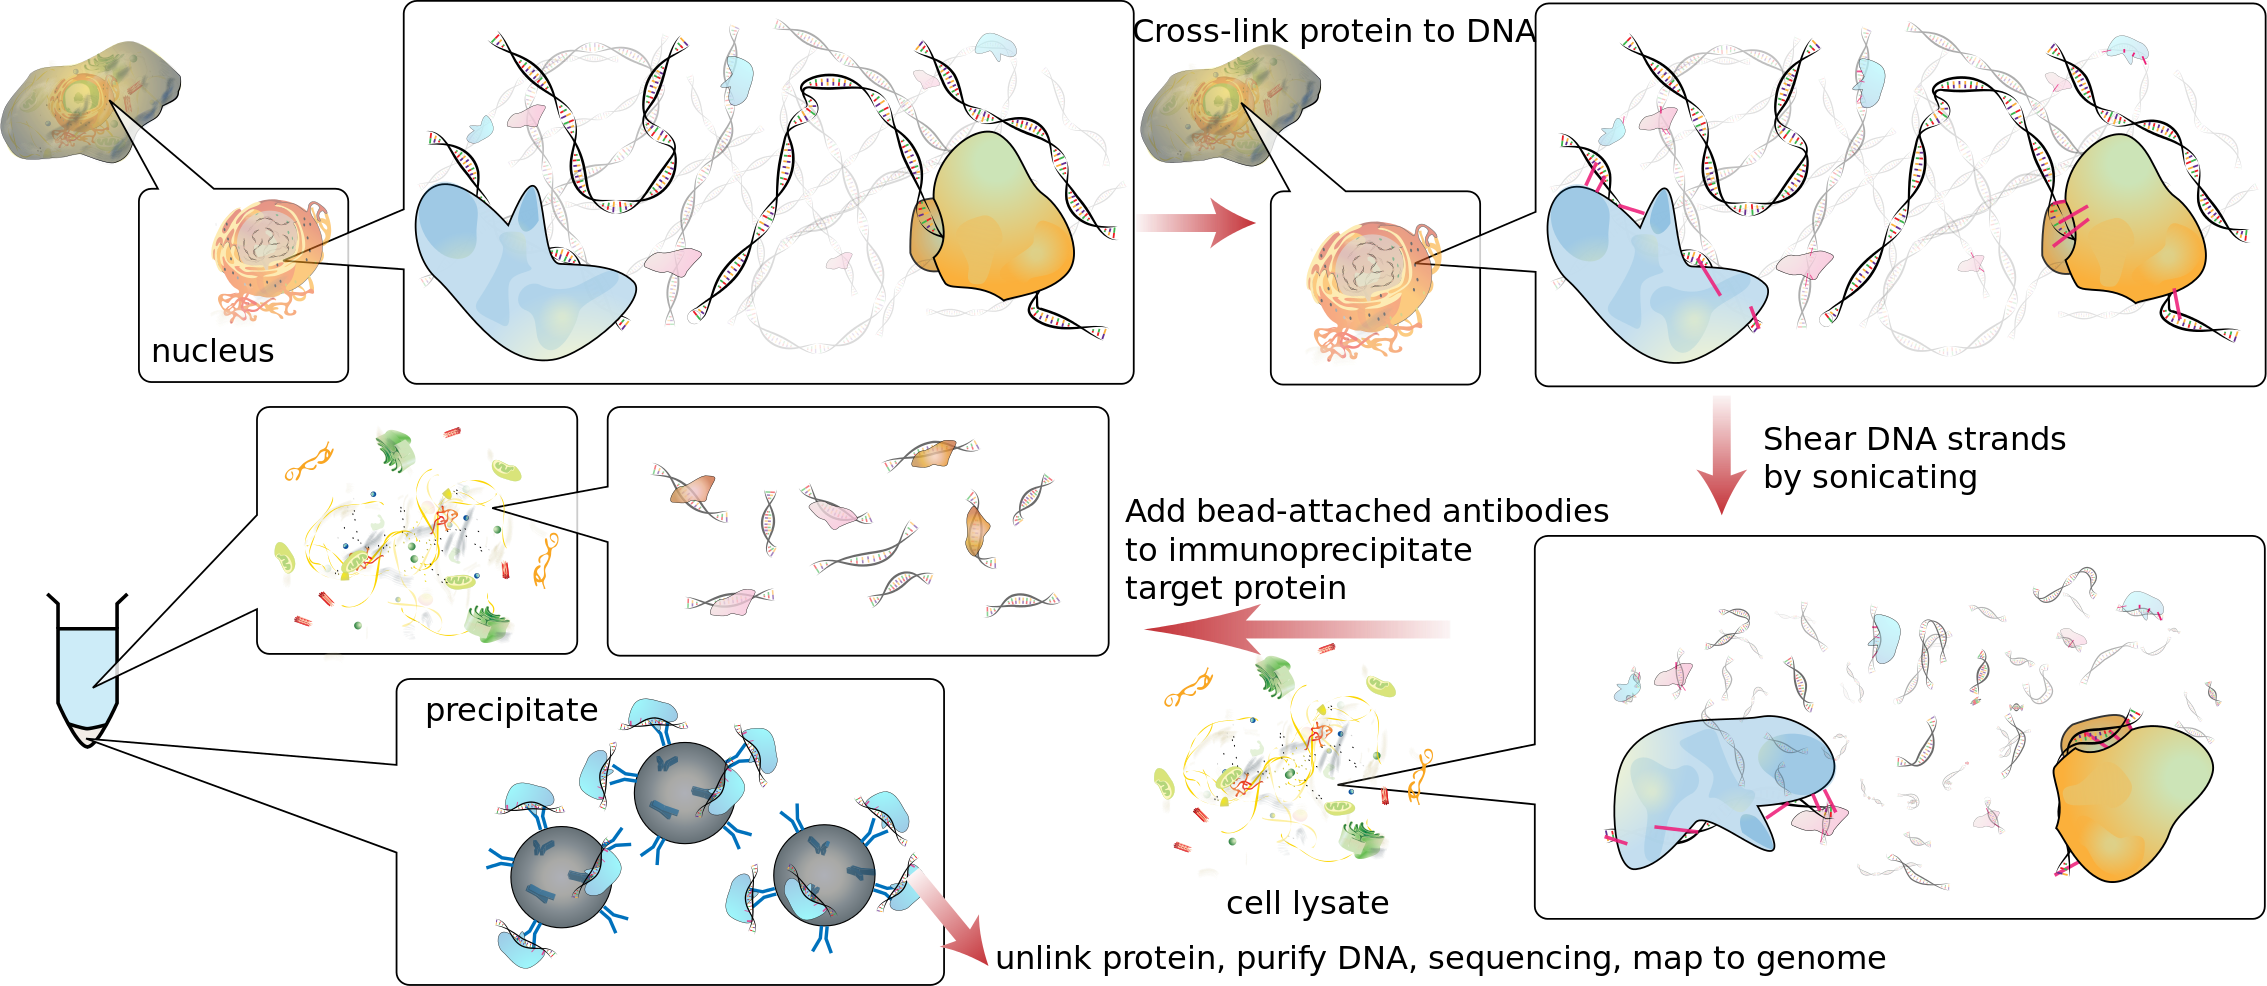
\includegraphics[width=\textwidth]{Chromatin_immunoprecipitation_sequencing_wide.png}

  Source: ``ChIP-sequencing,'' Wikipedia.
\end{frame}

\begin{frame}
  \frametitle{Problem: find peaks in each of several samples}
  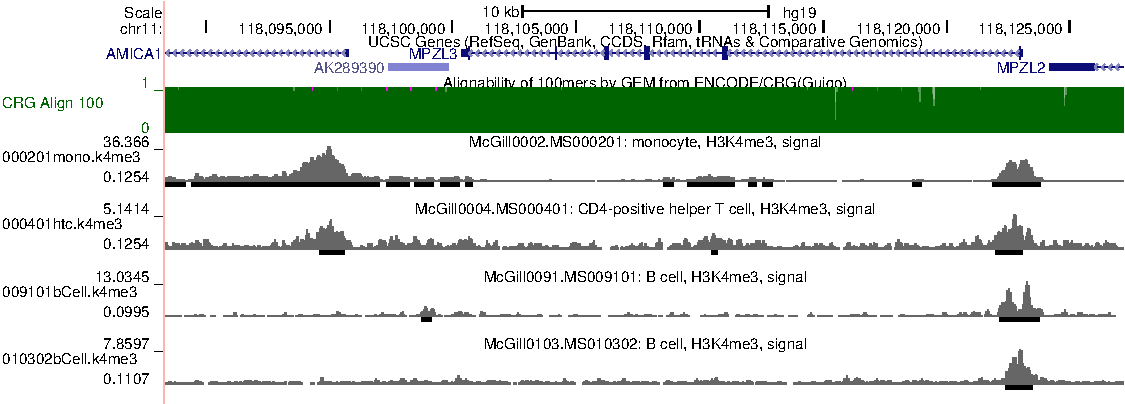
\includegraphics[width=\textwidth]{screenshot-ucsc-edited}

  \begin{itemize}
  \item Grey profiles are noisy aligned read count signals -- \\peaks
    are genomic locations with protein binding sites.
  \item Black bars are peaks called by MACS2 (Zhang et al, 2008) -- many
    false positives! (black bars where there is only noise)
  \item From a machine learning perspective, this is binary
    classification (positive=peaks, negative=noise).
  \end{itemize}
\end{frame}

% \begin{frame}
%   \frametitle{Previous work in genomic peak detection}
%   \begin{itemize}
%   \item Model-based analysis of ChIP-Seq (MACS), Zhang et al, 2008.
%   \item SICER, Zang et al, 2009.
%   \item HOMER, Heinz et al, 2010.
%   \item CCAT, Xu et al, 2010.
%   \item RSEG, Song et al, 2011.
%   \item Triform, Kornacker et al, 2012.
%   \item Histone modifications in cancer (HMCan), Ashoor et al, 2013.
%   \item PeakSeg, Hocking, Rigaill, Bourque, ICML 2015.
%   %\item PeakSegJoint Hocking and Bourque, arXiv:1506.01286.
%   \item ... dozens of others.
%   \end{itemize}
%   Two big questions: how to choose the best...
%   \begin{itemize}
%   \item ...algorithm? (testing)
%   \item \alert<1>{...parameters? (training)}
%   \end{itemize}
% \end{frame}

% \begin{frame}[fragile]
%   \frametitle{How to choose parameters of unsupervised peak
%     detectors?}
% \scriptsize
% 19 parameters for Model-based analysis of ChIP-Seq (MACS), Zhang et al, 2008.
% \begin{verbatim}
%   [-g GSIZE]
%   [-s TSIZE] [--bw BW] [-m MFOLD MFOLD] [--fix-bimodal]
%   [--nomodel] [--extsize EXTSIZE | --shiftsize SHIFTSIZE]
%   [-q QVALUE | -p PVALUE | -F FOLDENRICHMENT] [--to-large]
%   [--down-sample] [--seed SEED] [--nolambda]
%   [--slocal SMALLLOCAL] [--llocal LARGELOCAL]
%   [--shift-control] [--half-ext] [--broad]
%   [--broad-cutoff BROADCUTOFF] [--call-summits]
% \end{verbatim}
% 10 parameters for Histone modifications in cancer (HMCan),
% Ashoor et al, 2013.
% \begin{verbatim}
% minLength 145
% medLength 150
% maxLength 155
% smallBinLength 50
% largeBinLength 100000
% pvalueThreshold 0.01
% mergeDistance 200
% iterationThreshold 5
% finalThreshold 0
% maxIter 20
% \end{verbatim}
% \end{frame}
 
\begin{frame}
  \frametitle{Which macs parameter is best for these data?}
  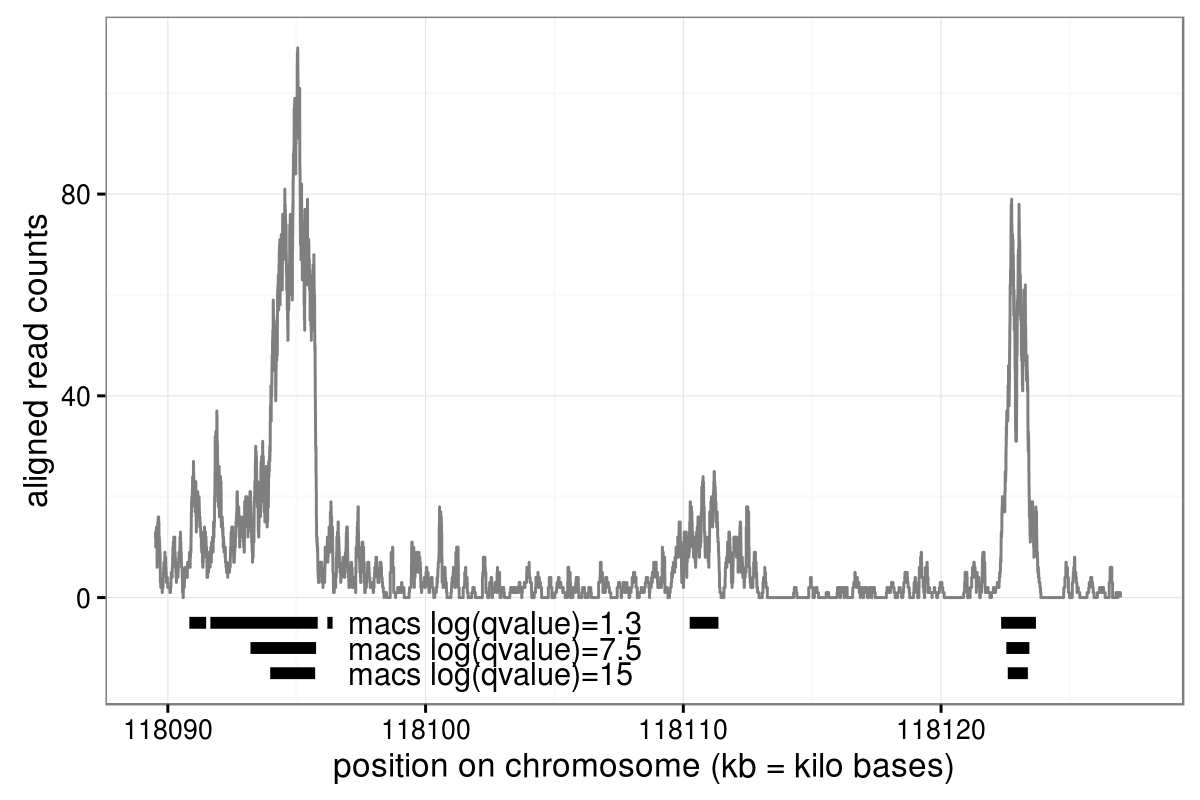
\includegraphics[width=1\textwidth]{figure-macs-problem.png}
\end{frame}

\begin{frame}
  \frametitle{Compute likelihood/loss of piecewise constant model}
  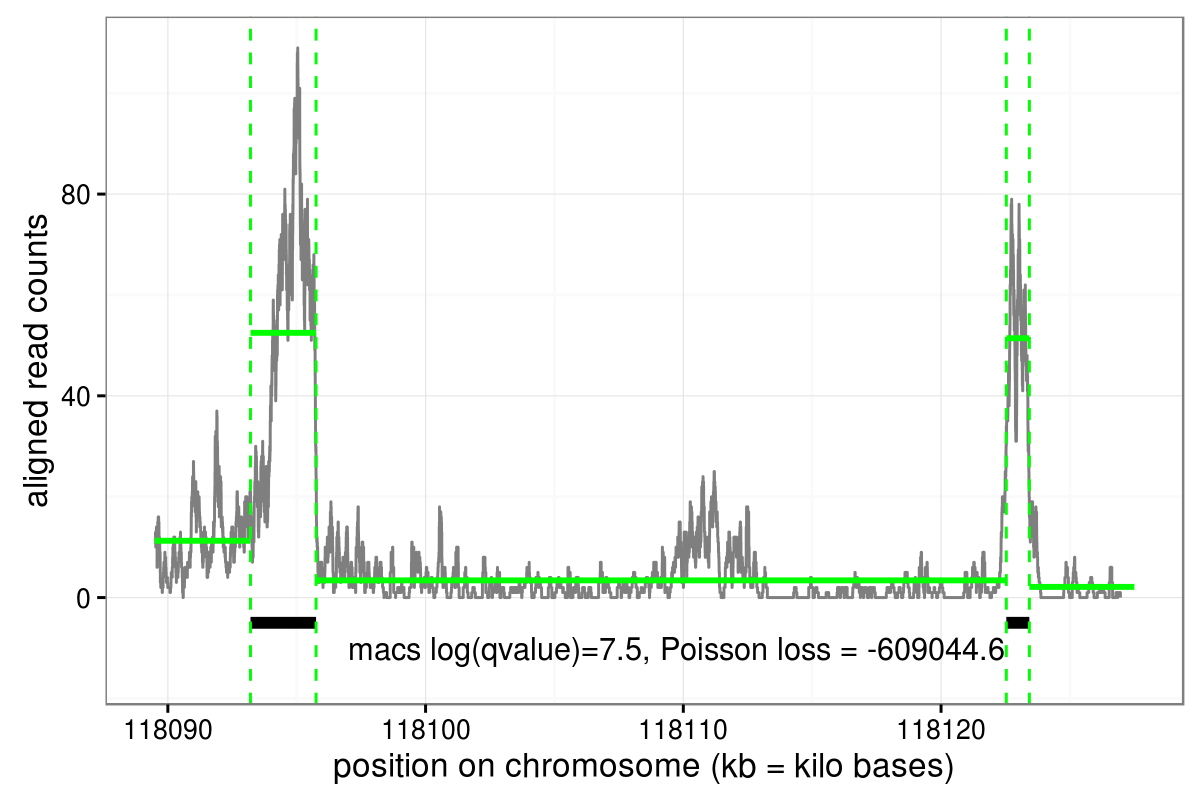
\includegraphics[width=1\textwidth]{figure-macs-problem-7-5.png}
  % $\PoissonLoss(\mathbf z, \mathbf m) = \sum_{i=1}^n m_i - z_i \log(m_i)$
  % for count data $\mathbf z\in\ZZ_+^n$ 
  % and segment mean model $\mathbf m\in\RR^n$.
\end{frame}

\begin{frame}
  \frametitle{Idea: choose the parameter with a lower loss}
  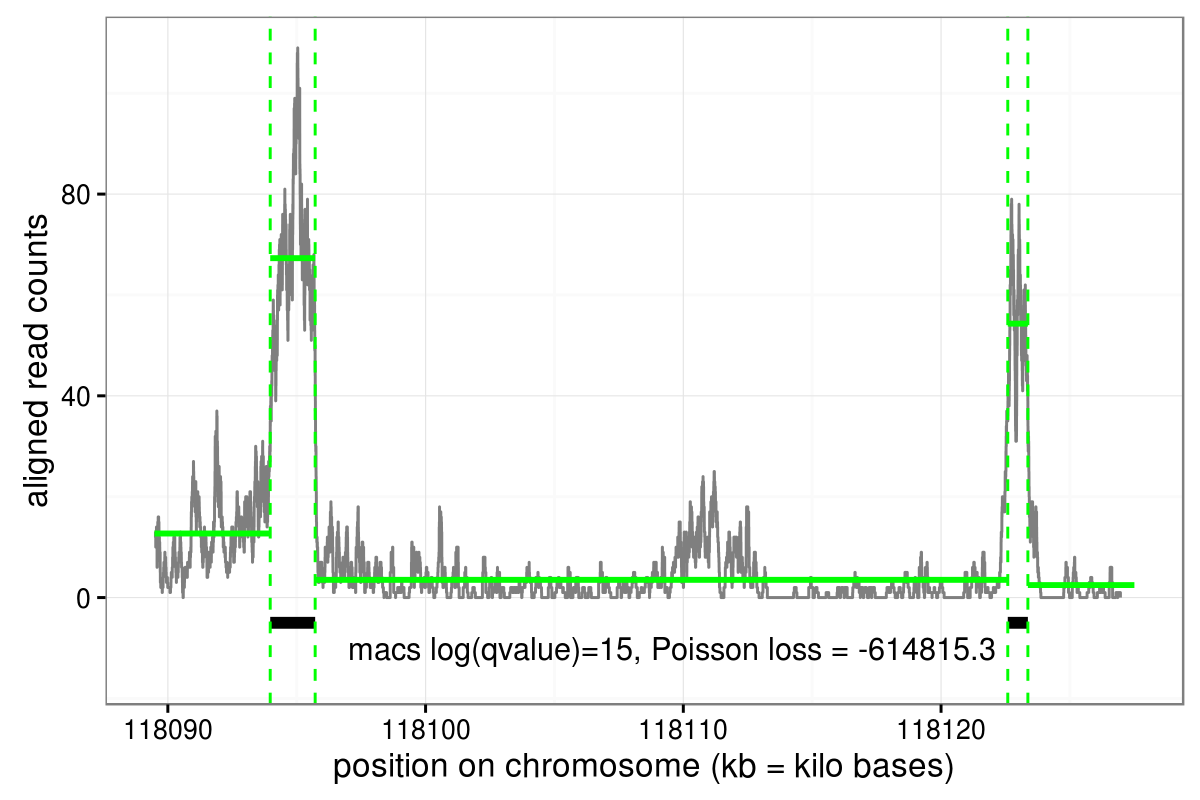
\includegraphics[width=1\textwidth]{figure-macs-problem-15.png}
\end{frame}

\begin{frame}
  \frametitle{PeakSeg: search for the peaks with lowest loss}
  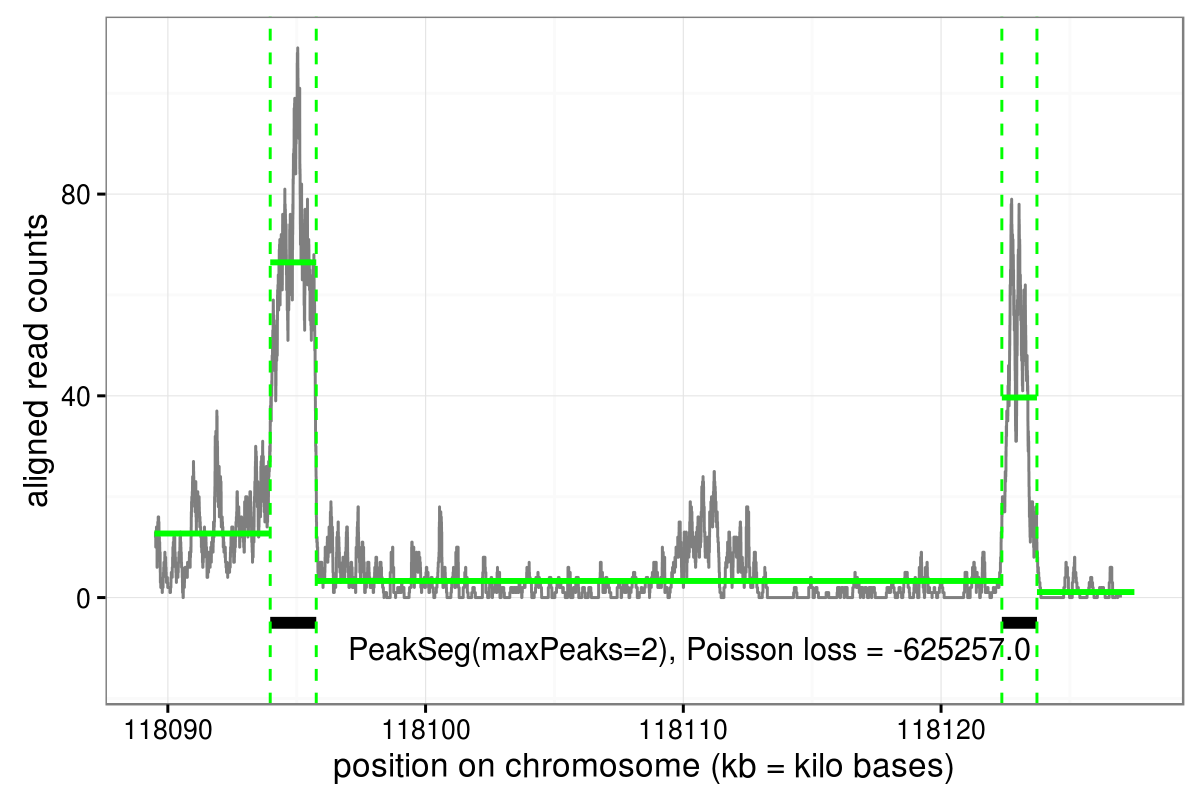
\includegraphics[width=1\textwidth]{figure-macs-problem-PeakSeg.png}

  Simple model with only one parameter (number of peaks).

  %Choose the number of peaks via standard penalties (AIC, BIC,
  %  ...)\\or learned penalties based on visual labels (more on this later).
\end{frame}

% \begin{frame}
%   \frametitle{Maximum likelihood Poisson segmentation models}
%   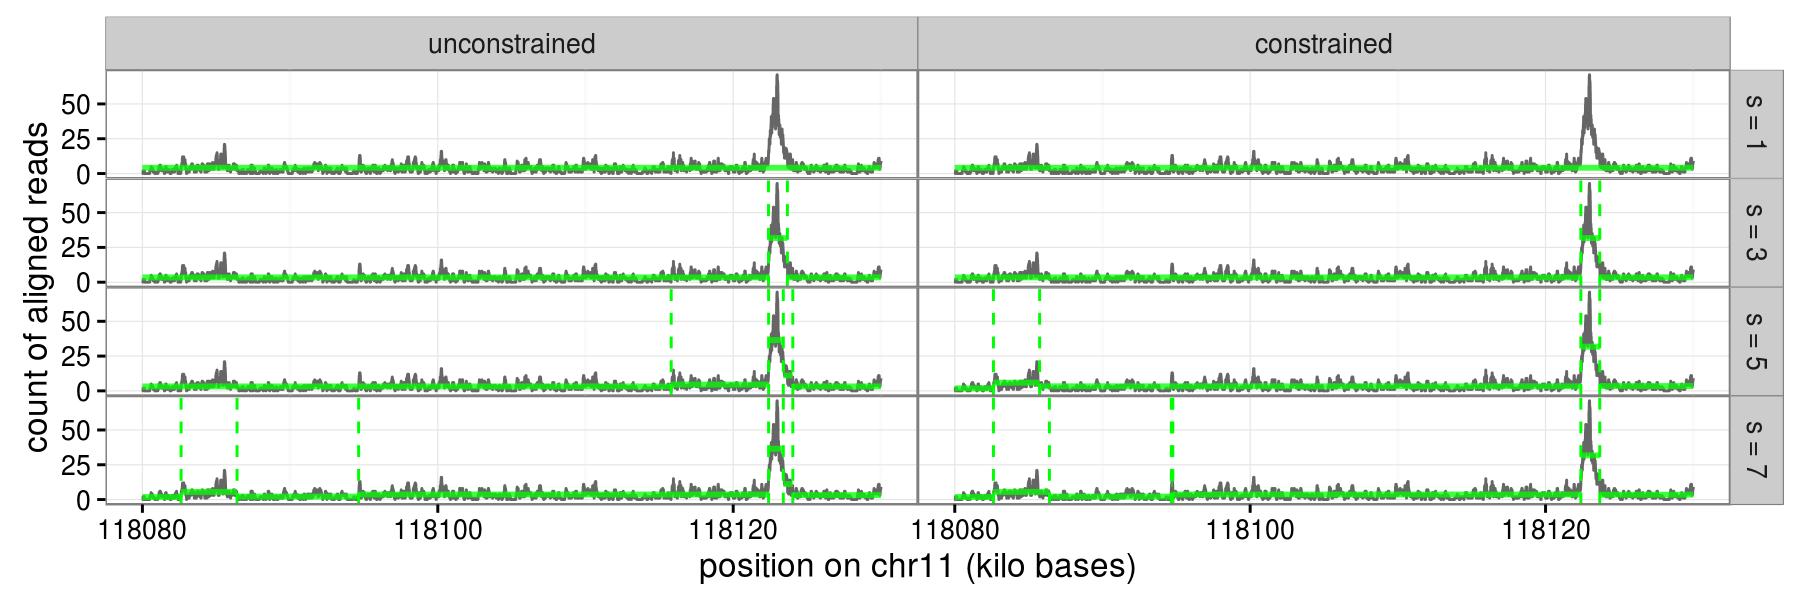
\includegraphics[width=1\textwidth]{figure-Segmentor-PeakSeg}

%   \begin{itemize}
%   \item Previous work: unconstrained maximum likelihood mean\\
%     for $s$ segments ($s-1$ changes), Cleynen et al 2014.
%   \item Hocking et al, ICML 2015: PeakSeg constraint enforces up, down, up,
%     down changes (and not up, up, down). 
%   \item Odd-numbered segments are background noise,\\
%     even-numbered segments are peaks.
%   \item Constrained Dynamic Programming Algorithm, $O(N^2)$ time for $N$ data points.
%   \end{itemize}
% \end{frame}

% \begin{frame}
%   \frametitle{But quadratic time is not fast enough for genomic data!}
%   \includegraphics[width=\textwidth]{figure-PDPA-timings-dp}
%   \begin{itemize}
%   \item Genomic data is large, $N \geq 10^6$.
%   \item Split into subsets? What if we split a peak in half?
%   \item Need linear time algorithm for analyzing whole data set.
%   \end{itemize}
% \end{frame}

% \begin{frame}
%   \frametitle{Statistical model is Poisson with change constraints}
%   \begin{itemize}
%   \item We have $N$ count data $z_1, \dots, z_N\in\ZZ_+$.
%   \item Fix the number of segments $S\in\{1, 2, \dots, N\}$.
%   \item PeakSeg Model: $z_t \sim \text{Poisson}(m_t)$ such that $m_t$
%     has $S-1$ up-down changes.
%   \item Want to find means $m_t$ which maximize the Poisson likelihood:
%     $P(Z = z_t|m_t) = m_t^{z_t} e^{-m_t} / (z_t!)$.
%   \item Equivalent to finding means $m_t$ which minimize the Poisson
%     loss: $\ell(m_t, z_t) = m_t - z_t\log m_t$.
%   \item Naive computation is $O(N^S)$, since there are $O(N^{S-1})$ possible
%     positions for $S-1$ change-points, and it takes $O(N)$ operations to
%     compute the mean and loss for each.
%   % \item Comparison to Hidden Markov Model:
%   %   \begin{description}
%   %   \item[Likelihood] Same emission terms, no transition terms.
%   %   \item[Constraint] Number of changes rather than values.
%   %   \end{description}
%   \end{itemize}
% \end{frame}

\begin{frame}
  \frametitle{Maximum likelihood changepoint detection with up-down constraints on adjacent segment means (PeakSeg)}
H {\it et al.}, {\it ICML} 2015. 
    
\only<1>{\input{figure-PeakSeg}}      
\only<2>{\input{figure-PeakSeg-unconstrained}}
\only<3>{\input{figure-PeakSeg-constrained}}
\vskip -1.5cm
\begin{align*}
    \minimize_{\substack{
  \mathbf u\in\RR^{S}
\\
   0=t_0<t_1<\cdots<t_{S-1}<t_S=n
  }} &\ \ 
    \sum_{s=1}^S\  \sum_{i=t_{s-1}+1}^{t_s} \ell( u_s,  x_i) 
  \label{PeakSegPDPA}
\\
      \text{subject to \hskip 0.75cm} &\ \ \alert<3>{u_{s-1} \leq u_s\ \forall s\in\{2,4,\dots\},}
  \nonumber\\
  &\ \ \alert<3>{u_{s-1} \geq u_s\ \forall s\in\{3,5,\dots\}.}
  \nonumber 
\end{align*}
\vskip -0.4cm
\begin{itemize}  
\item Simple: 1 parameter = number of segments $S\in\{1,3,\dots\}$.
\item Hard optimization problem, naively $O(n^S)$ time.
\item \alert<2>{Previous unconstrained model: not always up-down changes.}
\item \alert<3>{Interpretable: $P=(S-1)/2$ peaks (segments 2, 4, ...).}
\item New $O(Kn^2)$ time approximate algorithm based on classic
  dynamic programming (R package PeakSegDP).
\end{itemize}
\end{frame} 

\section{New functional pruning algorithm}


\begin{frame}
  \frametitle{Relation to previous work}
  \begin{tabular}{r|c|c}
    & no pruning & functional pruning \\
    \hline
    unconstrained & \alert<1>{Dynamic Prog. Algo.} & \alert<2>{Pruned DPA} \\
     & \alert<1>{exact $O(SN^2)$} & \alert<2>{exact $O(SN\log N)$}\\
    R pkgs: & \alert<1>{changepoint} & \alert<2>{cghseg, Segmentor}\\
    \hline
    up-down constrained & \alert<3>{Constrained DPA} & \alert<4>{\textbf{GPDPA}} \\
     & \alert<3>{inexact $O(SN^2)$} & \alert<4>{exact $O(SN\log N)$}\\
    R pkgs: & \alert<3>{PeakSegDP} & \alert<4>{PeakSegOptimal}\\
    \hline
  \end{tabular}
  \begin{itemize}
  \item \alert<1>{Auger and Lawrence 1989, Jackson et al 2005}.
  \item \alert<2>{Rigaill 2010, Johnson 2013, Cleynen et al 2014}.
  \item \alert<3>{Hocking, Rigaill, Bourque 2015}.
  \item \alert<4>{\textbf{Contribution:} Generalized Pruned Dynamic
        Programming Algorithm (GPDPA) that \textbf{exactly} computes the
      \textbf{constrained} model for $N$ data points and up to $S$ segments in
       $O(SN\log N)$ time}.
  \end{itemize}
\end{frame}

\begin{frame}
  \frametitle{Dynamic programming and functional pruning}
  \textbf{Classical dynamic programming} (Auger and Lawrence 1989)
  computes the matrix of optimal loss values in $S$ segments up to $N$
  data points, $O(S N^2)$
$$
\begin{array}{ccc}
  \mathcal L_{1,1} & \cdots &   \mathcal L_{1,N}\\
  \vdots &  & \vdots\\
  \mathcal L_{S,1} & \cdots & \mathcal L_{S,N}\\
\end{array}
$$
\textbf{Dynamic programming with functional pruning} (Rigaill 2010,
Johnson 2013) computes a matrix of loss \textbf{functions}, the
optimal loss up to $N$ data points if segment $S$ has mean $\mu_S$,
$O(S N\log N)$
$$
\begin{array}{ccc}
   L_{1,1}(\mu_1) & \cdots & L_{1,N}(\mu_1)\\
  \vdots &  & \vdots\\
   L_{S,1}(\mu_S) & \cdots & L_{S,N}(\mu_S),\\
\end{array}
$$
\textbf{Contribution of this work}: a new algorithm that applies the
functional pruning technique to the up-down constrained model.
\end{frame}

\begin{frame}
  \frametitle{First segment, first data point}
  \begin{itemize}
  \item For data $z_1, \dots, z_N\in\ZZ_+$ let
  \begin{equation*}
    \gamma_t(\mu) = \ell(\mu, z_t) = \mu - z_t \log \mu
  \end{equation*}
  be the Poisson loss for each $t\in\{1, \dots, N\}$.
\item For example $z = 2, 1, 0, 4$.
\item Then $\gamma_1(\mu)=L_{1,1}(\mu)= \alert{1}\mu - \alert{2}\log \mu + \alert{0}$.
\item Need to store 3 coefficients (\alert{linear}, \alert{log}, \alert{constant}).
  \end{itemize}
  \begin{center}
    \includegraphics[width=0.7\textwidth]{figure-PeakSegPDPA-demo-cost-1segments-1data}
  \end{center}
\end{frame}

\begin{frame}
  \frametitle{First segment, other data points}
  \begin{itemize}
\item
  The loss of the first segment up to data point $t$ is
  \begin{equation*}
    \label{eq:C1b}
    L_{1,t}(\mu) = \sum_{i=1}^t \gamma_i(\mu).
  \end{equation*}
\item For example $z = 2, 1, 0, 4$.
% \item $L_{1,2}(\mu) = (2\mu - 3\log\mu + 0)/2 = 1\mu - 1.5\log\mu + 0$.
% \item $L_{1,3}(\mu) = (3\mu - 13\log\mu + 0)/3 = 1\mu - 4.333\log\mu + 0$.
\item $L_{1,2}(\mu) = 2\mu - 3\log\mu + 0$.
\item $L_{1,3}(\mu) = 3\mu - 12\log\mu + 0$.
\item ...
  \end{itemize}
  \begin{center}
    \includegraphics[width=0.5\textwidth]{figure-PeakSegPDPA-demo-cost-1segments-2data}
    \includegraphics[width=0.5\textwidth]{figure-PeakSegPDPA-demo-cost-1segments-3data}
  \end{center}
\end{frame}

\begin{frame}[fragile]
  \frametitle{Second segment, up to data point 2}
  \begin{itemize}
  \item The cost in 2 segments up to data point 2 is
\begin{eqnarray*}
  L_{2,2}(\mu_2) 
  &=&  \gamma_2(\mu_2)+\min_{\mu_1 \leq \mu_2} L_{1,1}(\mu_1)\\
  &=& \gamma_2(\mu_2)+L_{1,1}^{\leq}(\mu_2)
\end{eqnarray*}
\item Min-less operator $L^\leq(\mu) = \min_{x\leq\mu} L(x)$ can be
  computed and stored exactly for every possible $\mu$!
    \begin{center}
      \includegraphics[width=0.5\textwidth]{figure-PeakSegPDPA-demo-minlessmore-2segments-2data}
    \end{center}
\end{itemize}
\end{frame}

\begin{frame}
  \frametitle{Comparison with unconstrained Pruned DPA}
  \begin{itemize}
  \item For our constrained algorithm, the first segment mean must be
    less than the second, and the first segment cost is a function:
    \begin{equation*}
      L_{2,2}(\mu_2) = \gamma_2(\mu_2)+
      \underbrace{\min_{\mu_1 \leq \mu_2} L_{1,1}(\mu_1)}_{L^\leq_{1,1}(\mu_2)}.
    \end{equation*}
  \item For the unconstrained algorithm, it is \alert<1>{constant}:
    \begin{equation*}
      \widehat{L}_{2,2}(\mu_2) = \gamma_2(\mu_2)+
      \alert<1>{\underbrace{\min_{\mu_1} L_{1,1}(\mu_1)}_{\mathcal L_{1,1}}}.
    \end{equation*}
  \item For example $z = 2, 1, 0, 4$.
    \begin{center}
      \includegraphics[width=0.5\textwidth]{figure-PeakSegPDPA-demo-mincompare-2segments-2data}
    \end{center}
  \end{itemize}
\end{frame}

\begin{frame}
  \frametitle{Storage as a piecewise function on intervals}
  \begin{itemize}
  \item For example $z = 2, 1, 0, 4$.
    \begin{center}
      \includegraphics[width=0.5\textwidth]{figure-PeakSegPDPA-demo-minlessmore-2segments-2data}
    \end{center}
  \item Storage: coefficients, intervals, previous segment mean,
    $L_{2,2}(\mu) = \gamma_2(\mu) +$
    \begin{equation*}
      \begin{cases}
        %L_{1,1}(\mu) = 
        1\mu - 2\log \mu + 0 & \text{ if } \mu\in[0, 2],\, \mu'=\mu\\
        %\mathcal L_{1,1} = 
        0\mu -0\log\mu + 0.6137 & \text{ if } \mu\in[2, 4],\, \mu'=2.
      \end{cases}
    \end{equation*}
  \end{itemize}
\end{frame}

 
\begin{frame}[fragile]
  \frametitle{Second segment, up to data point 3}
  \begin{itemize}
  \item For data point 3 we need to consider two change-points:
    \begin{equation*}
      L_{2,3}(\mu) =  \gamma_3(\mu) + \min
      \begin{cases}
        L_{1,2}^{\leq}(\mu), & \text{ change up after data point 2},\\
        L_{2,2}(\mu), & \text{ change up after data point 1}. 
      \end{cases}
    \end{equation*}
  \item For $z = 2, 1, 0, 4$ the min operation prunes a
    change after data point 1.
    \begin{center}
      \includegraphics[width=0.5\textwidth]{figure-PeakSegPDPA-demo-minenv-2segments-3data}
    \end{center}
  \end{itemize}
\end{frame}

\begin{frame}
  \frametitle{Second segment, up to data point t}
  \begin{itemize}
  \item The updates continue for every data point $t\in\{3, ..., N\}$
    \begin{eqnarray*}
      L_{2,t}(\mu) &=&  \gamma_t(\mu) + \min
      \begin{cases}
        L_{1,t-1}^{\leq}(\mu), & \text{change up after $t-1$,}\\
        L_{2,t-1}(\mu), & \text{change up before $t-1$.}
      \end{cases}
% \\
%       &=& \min_{\tau\in\{1,2,\dots,t-1\}} c_{2,t,\tau}(\mu)
%           = \min_{\tau\in T_{2,t}} c_{2,t,\tau}(\mu)
    \end{eqnarray*}
  \item For example for $z = 2, 1, 0, 4$, at data point $t=4$
    we only need to consider changes after 2 and 3 (1 has been
    pruned).
% $$
% L_{2,4}(\mu) &=& \min_{\tau\in\{1,2,3\}} c_{2,t,\tau} = 
% \min_{\tau\in\{2,3\}} c_{2,t,\tau} 
% $$
    \begin{center}
      \includegraphics[width=0.5\textwidth]{figure-PeakSegPDPA-demo-minenv-2segments-4data}
    \end{center}
  \end{itemize}
\end{frame}


\begin{frame}
  \frametitle{Generalized pruned dynamic programming algorithm (GPDPA)}
  Dynamic programming update rule: the constrained cost of a
  mean $\mu$ for the segment $s$, up to data point $t$.
  \begin{itemize}
  \item For $s=2, 4, \dots$
    \begin{equation*}
      L_{s,t}(\mu) = \gamma_t(\mu) + \min
      \begin{cases}
        L_{s,t-1}(\mu),\\
        L_{s-1,t-1}^{\alert{\leq}}(\mu),
      \end{cases}
    \end{equation*}
  \item For $s=3, 5, \dots$
    \begin{equation*}
      L_{s,t}(\mu) = \gamma_t(\mu) + \min
      \begin{cases}
        L_{s,t-1}(\mu),\\
        L_{s-1,t-1}^{\alert{\geq}}(\mu),
      \end{cases}
    \end{equation*}
  \end{itemize}
\end{frame}

\begin{frame}
  \frametitle{More complex $\min\{\}$ computation}
  Time/space complexity linear in number of intervals (candidate changepoints).
  \begin{minipage}[t]{\linewidth}
  \hskip -1cm
  % Created by tikzDevice version 0.10.1 on 2017-02-20 09:55:27
% !TEX encoding = UTF-8 Unicode
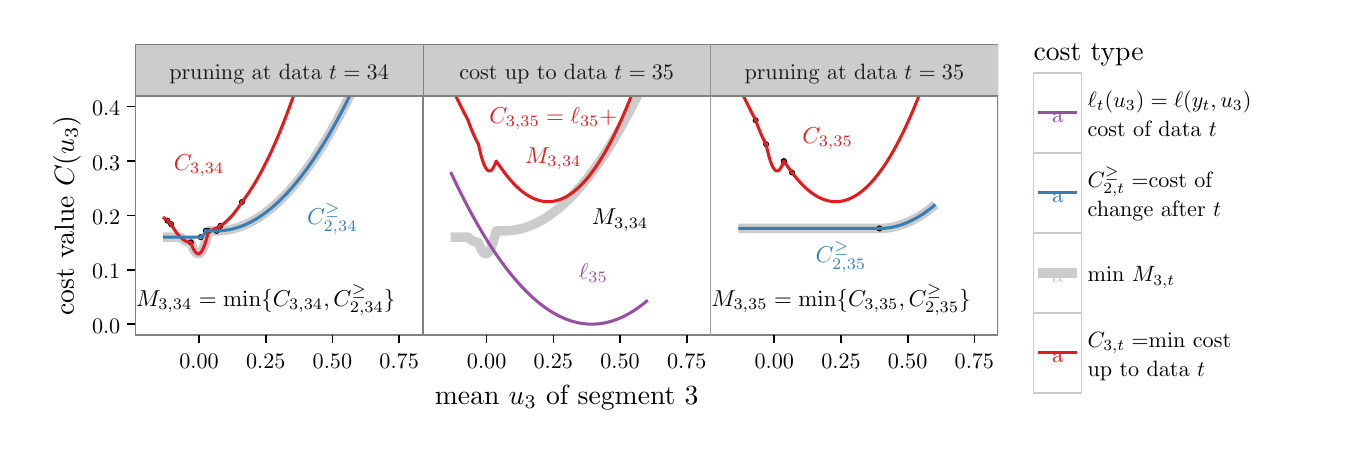
\begin{tikzpicture}[x=1pt,y=1pt]
\definecolor{fillColor}{RGB}{255,255,255}
\path[use as bounding box,fill=fillColor,fill opacity=0.00] (0,0) rectangle (469.75,144.54);
\begin{scope}
\path[clip] (  0.00,  0.00) rectangle (469.75,144.54);
\definecolor{drawColor}{RGB}{255,255,255}
\definecolor{fillColor}{RGB}{255,255,255}

\path[draw=drawColor,line width= 0.6pt,line join=round,line cap=round,fill=fillColor] (  0.00, -0.00) rectangle (469.76,144.54);
\end{scope}
\begin{scope}
\path[clip] ( 38.87,119.93) rectangle (142.81,138.54);
\definecolor{drawColor}{gray}{0.50}
\definecolor{fillColor}{gray}{0.80}

\path[draw=drawColor,line width= 0.2pt,line join=round,line cap=round,fill=fillColor] ( 38.87,119.93) rectangle (142.81,138.54);
\definecolor{drawColor}{gray}{0.10}

\node[text=drawColor,anchor=base,inner sep=0pt, outer sep=0pt, scale=  0.80] at ( 90.84,125.93) {pruning at data $t=34$};
\end{scope}
\begin{scope}
\path[clip] (142.81,119.93) rectangle (246.74,138.54);
\definecolor{drawColor}{gray}{0.50}
\definecolor{fillColor}{gray}{0.80}

\path[draw=drawColor,line width= 0.2pt,line join=round,line cap=round,fill=fillColor] (142.81,119.93) rectangle (246.74,138.54);
\definecolor{drawColor}{gray}{0.10}

\node[text=drawColor,anchor=base,inner sep=0pt, outer sep=0pt, scale=  0.80] at (194.77,125.93) {cost up to data $t=35$};
\end{scope}
\begin{scope}
\path[clip] (246.74,119.93) rectangle (350.67,138.54);
\definecolor{drawColor}{gray}{0.50}
\definecolor{fillColor}{gray}{0.80}

\path[draw=drawColor,line width= 0.2pt,line join=round,line cap=round,fill=fillColor] (246.74,119.93) rectangle (350.67,138.54);
\definecolor{drawColor}{gray}{0.10}

\node[text=drawColor,anchor=base,inner sep=0pt, outer sep=0pt, scale=  0.80] at (298.71,125.93) {pruning at data $t=35$};
\end{scope}
\begin{scope}
\path[clip] ( 38.87, 33.48) rectangle (142.81,119.93);
\definecolor{fillColor}{RGB}{255,255,255}

\path[fill=fillColor] ( 38.87, 33.48) rectangle (142.81,119.93);
\definecolor{drawColor}{gray}{0.80}

\path[draw=drawColor,line width= 3.4pt,line join=round] ( 48.91, 68.84) --
	( 48.98, 68.84) --
	( 49.04, 68.84) --
	( 49.10, 68.84) --
	( 49.17, 68.84) --
	( 49.23, 68.84) --
	( 49.29, 68.84) --
	( 49.36, 68.84) --
	( 49.42, 68.84) --
	( 49.48, 68.84) --
	( 49.55, 68.84) --
	( 49.61, 68.84) --
	( 49.67, 68.84) --
	( 49.74, 68.84) --
	( 49.80, 68.84) --
	( 49.86, 68.84) --
	( 49.93, 68.84) --
	( 49.99, 68.84) --
	( 50.06, 68.84) --
	( 50.12, 68.84) --
	( 50.18, 68.84) --
	( 50.25, 68.84) --
	( 50.31, 68.84) --
	( 50.37, 68.84) --
	( 50.44, 68.84) --
	( 50.50, 68.84) --
	( 50.56, 68.84) --
	( 50.63, 68.84) --
	( 50.69, 68.84) --
	( 50.75, 68.84) --
	( 50.82, 68.84) --
	( 50.88, 68.84) --
	( 50.94, 68.84) --
	( 51.01, 68.84) --
	( 51.07, 68.84) --
	( 51.14, 68.84) --
	( 51.20, 68.84) --
	( 51.26, 68.84) --
	( 51.33, 68.84) --
	( 51.39, 68.84) --
	( 51.45, 68.84) --
	( 51.52, 68.84) --
	( 51.58, 68.84) --
	( 51.64, 68.84) --
	( 51.71, 68.84) --
	( 51.77, 68.84) --
	( 51.83, 68.84) --
	( 51.90, 68.84) --
	( 51.96, 68.84) --
	( 52.02, 68.84) --
	( 52.09, 68.84) --
	( 52.15, 68.84) --
	( 52.22, 68.84) --
	( 52.28, 68.84) --
	( 52.34, 68.84) --
	( 52.41, 68.84) --
	( 52.47, 68.84) --
	( 52.53, 68.84) --
	( 52.60, 68.84) --
	( 52.66, 68.84) --
	( 52.72, 68.84) --
	( 52.79, 68.84) --
	( 52.85, 68.84) --
	( 52.91, 68.84) --
	( 52.98, 68.84) --
	( 53.04, 68.84) --
	( 53.10, 68.84) --
	( 53.17, 68.84) --
	( 53.23, 68.84) --
	( 53.30, 68.84) --
	( 53.36, 68.84) --
	( 53.42, 68.84) --
	( 53.49, 68.84) --
	( 53.55, 68.84) --
	( 53.61, 68.84) --
	( 53.68, 68.84) --
	( 53.74, 68.84) --
	( 53.80, 68.84) --
	( 53.87, 68.84) --
	( 53.93, 68.84) --
	( 53.99, 68.84) --
	( 54.06, 68.84) --
	( 54.12, 68.84) --
	( 54.18, 68.84) --
	( 54.25, 68.84) --
	( 54.31, 68.84) --
	( 54.38, 68.84) --
	( 54.44, 68.84) --
	( 54.50, 68.84) --
	( 54.57, 68.84) --
	( 54.63, 68.84) --
	( 54.69, 68.84) --
	( 54.76, 68.84) --
	( 54.82, 68.84) --
	( 54.88, 68.84) --
	( 54.95, 68.84) --
	( 55.01, 68.84) --
	( 55.07, 68.84) --
	( 55.14, 68.84) --
	( 55.20, 68.84) --
	( 55.20, 68.84) --
	( 55.24, 68.80) --
	( 55.28, 68.76) --
	( 55.32, 68.73) --
	( 55.35, 68.69) --
	( 55.39, 68.66) --
	( 55.43, 68.62) --
	( 55.47, 68.59) --
	( 55.51, 68.55) --
	( 55.54, 68.52) --
	( 55.58, 68.48) --
	( 55.62, 68.45) --
	( 55.66, 68.42) --
	( 55.69, 68.39) --
	( 55.73, 68.35) --
	( 55.77, 68.32) --
	( 55.81, 68.29) --
	( 55.85, 68.26) --
	( 55.88, 68.23) --
	( 55.92, 68.20) --
	( 55.96, 68.17) --
	( 56.00, 68.14) --
	( 56.04, 68.11) --
	( 56.07, 68.08) --
	( 56.11, 68.05) --
	( 56.15, 68.02) --
	( 56.19, 68.00) --
	( 56.23, 67.97) --
	( 56.26, 67.94) --
	( 56.30, 67.92) --
	( 56.34, 67.89) --
	( 56.38, 67.86) --
	( 56.42, 67.84) --
	( 56.45, 67.81) --
	( 56.49, 67.79) --
	( 56.53, 67.76) --
	( 56.57, 67.74) --
	( 56.61, 67.72) --
	( 56.64, 67.69) --
	( 56.68, 67.67) --
	( 56.72, 67.65) --
	( 56.76, 67.62) --
	( 56.80, 67.60) --
	( 56.83, 67.58) --
	( 56.87, 67.56) --
	( 56.91, 67.54) --
	( 56.95, 67.52) --
	( 56.99, 67.50) --
	( 57.02, 67.48) --
	( 57.06, 67.46) --
	( 57.10, 67.44) --
	( 57.14, 67.42) --
	( 57.17, 67.40) --
	( 57.21, 67.39) --
	( 57.25, 67.37) --
	( 57.29, 67.35) --
	( 57.33, 67.33) --
	( 57.36, 67.32) --
	( 57.40, 67.30) --
	( 57.44, 67.29) --
	( 57.48, 67.27) --
	( 57.52, 67.26) --
	( 57.55, 67.24) --
	( 57.59, 67.23) --
	( 57.63, 67.21) --
	( 57.67, 67.20) --
	( 57.71, 67.19) --
	( 57.74, 67.17) --
	( 57.78, 67.16) --
	( 57.82, 67.15) --
	( 57.86, 67.14) --
	( 57.90, 67.13) --
	( 57.93, 67.11) --
	( 57.97, 67.10) --
	( 58.01, 67.09) --
	( 58.05, 67.08) --
	( 58.09, 67.07) --
	( 58.12, 67.07) --
	( 58.16, 67.06) --
	( 58.20, 67.05) --
	( 58.24, 67.04) --
	( 58.28, 67.03) --
	( 58.31, 67.03) --
	( 58.35, 67.02) --
	( 58.39, 67.01) --
	( 58.43, 67.01) --
	( 58.47, 67.00) --
	( 58.50, 66.99) --
	( 58.54, 66.99) --
	( 58.58, 66.98) --
	( 58.62, 66.98) --
	( 58.65, 66.98) --
	( 58.69, 66.97) --
	( 58.73, 66.97) --
	( 58.77, 66.97) --
	( 58.81, 66.96) --
	( 58.84, 66.96) --
	( 58.88, 66.96) --
	( 58.92, 66.96) --
	( 58.96, 66.96) --
	( 58.96, 66.96) --
	( 59.02, 66.76) --
	( 59.09, 66.56) --
	( 59.15, 66.38) --
	( 59.22, 66.19) --
	( 59.28, 66.01) --
	( 59.34, 65.84) --
	( 59.41, 65.67) --
	( 59.47, 65.50) --
	( 59.54, 65.34) --
	( 59.60, 65.19) --
	( 59.67, 65.04) --
	( 59.73, 64.89) --
	( 59.80, 64.75) --
	( 59.86, 64.62) --
	( 59.92, 64.49) --
	( 59.99, 64.36) --
	( 60.05, 64.24) --
	( 60.12, 64.13) --
	( 60.18, 64.02) --
	( 60.25, 63.91) --
	( 60.31, 63.81) --
	( 60.38, 63.72) --
	( 60.44, 63.62) --
	( 60.50, 63.54) --
	( 60.57, 63.46) --
	( 60.63, 63.38) --
	( 60.70, 63.31) --
	( 60.76, 63.24) --
	( 60.83, 63.18) --
	( 60.89, 63.12) --
	( 60.95, 63.07) --
	( 61.02, 63.03) --
	( 61.08, 62.98) --
	( 61.15, 62.95) --
	( 61.21, 62.92) --
	( 61.28, 62.89) --
	( 61.34, 62.87) --
	( 61.41, 62.85) --
	( 61.47, 62.84) --
	( 61.53, 62.83) --
	( 61.60, 62.83) --
	( 61.66, 62.83) --
	( 61.73, 62.84) --
	( 61.79, 62.85) --
	( 61.86, 62.86) --
	( 61.92, 62.89) --
	( 61.98, 62.91) --
	( 62.05, 62.95) --
	( 62.11, 62.98) --
	( 62.18, 63.02) --
	( 62.24, 63.07) --
	( 62.31, 63.12) --
	( 62.37, 63.18) --
	( 62.44, 63.24) --
	( 62.50, 63.30) --
	( 62.56, 63.38) --
	( 62.63, 63.45) --
	( 62.69, 63.53) --
	( 62.76, 63.62) --
	( 62.82, 63.71) --
	( 62.89, 63.80) --
	( 62.95, 63.90) --
	( 63.01, 64.01) --
	( 63.08, 64.12) --
	( 63.14, 64.24) --
	( 63.21, 64.36) --
	( 63.27, 64.48) --
	( 63.34, 64.61) --
	( 63.40, 64.75) --
	( 63.47, 64.88) --
	( 63.53, 65.03) --
	( 63.59, 65.18) --
	( 63.66, 65.33) --
	( 63.72, 65.49) --
	( 63.79, 65.66) --
	( 63.85, 65.83) --
	( 63.92, 66.00) --
	( 63.98, 66.18) --
	( 64.05, 66.36) --
	( 64.11, 66.55) --
	( 64.17, 66.75) --
	( 64.24, 66.94) --
	( 64.30, 67.15) --
	( 64.37, 67.36) --
	( 64.43, 67.57) --
	( 64.50, 67.79) --
	( 64.56, 68.01) --
	( 64.62, 68.24) --
	( 64.69, 68.47) --
	( 64.75, 68.71) --
	( 64.82, 68.95) --
	( 64.88, 69.20) --
	( 64.95, 69.45) --
	( 65.01, 69.71) --
	( 65.08, 69.97) --
	( 65.14, 70.24) --
	( 65.20, 70.51) --
	( 65.27, 70.79) --
	( 65.33, 71.07) --
	( 65.33, 71.07) --
	( 65.33, 71.07) --
	( 65.34, 71.07) --
	( 65.34, 71.07) --
	( 65.34, 71.07) --
	( 65.34, 71.07) --
	( 65.35, 71.07) --
	( 65.35, 71.07) --
	( 65.35, 71.07) --
	( 65.35, 71.08) --
	( 65.35, 71.08) --
	( 65.36, 71.08) --
	( 65.36, 71.08) --
	( 65.36, 71.08) --
	( 65.36, 71.08) --
	( 65.36, 71.08) --
	( 65.37, 71.08) --
	( 65.37, 71.08) --
	( 65.37, 71.08) --
	( 65.37, 71.08) --
	( 65.37, 71.08) --
	( 65.38, 71.08) --
	( 65.38, 71.08) --
	( 65.38, 71.08) --
	( 65.38, 71.08) --
	( 65.38, 71.08) --
	( 65.39, 71.08) --
	( 65.39, 71.08) --
	( 65.39, 71.08) --
	( 65.39, 71.09) --
	( 65.39, 71.09) --
	( 65.40, 71.09) --
	( 65.40, 71.09) --
	( 65.40, 71.09) --
	( 65.40, 71.09) --
	( 65.40, 71.09) --
	( 65.41, 71.09) --
	( 65.41, 71.09) --
	( 65.41, 71.09) --
	( 65.41, 71.09) --
	( 65.41, 71.09) --
	( 65.42, 71.09) --
	( 65.42, 71.09) --
	( 65.42, 71.09) --
	( 65.42, 71.09) --
	( 65.42, 71.09) --
	( 65.43, 71.09) --
	( 65.43, 71.09) --
	( 65.43, 71.10) --
	( 65.43, 71.10) --
	( 65.43, 71.10) --
	( 65.44, 71.10) --
	( 65.44, 71.10) --
	( 65.44, 71.10) --
	( 65.44, 71.10) --
	( 65.44, 71.10) --
	( 65.45, 71.10) --
	( 65.45, 71.10) --
	( 65.45, 71.10) --
	( 65.45, 71.10) --
	( 65.46, 71.10) --
	( 65.46, 71.10) --
	( 65.46, 71.10) --
	( 65.46, 71.10) --
	( 65.46, 71.10) --
	( 65.47, 71.10) --
	( 65.47, 71.10) --
	( 65.47, 71.11) --
	( 65.47, 71.11) --
	( 65.47, 71.11) --
	( 65.48, 71.11) --
	( 65.48, 71.11) --
	( 65.48, 71.11) --
	( 65.48, 71.11) --
	( 65.48, 71.11) --
	( 65.49, 71.11) --
	( 65.49, 71.11) --
	( 65.49, 71.11) --
	( 65.49, 71.11) --
	( 65.49, 71.11) --
	( 65.50, 71.11) --
	( 65.50, 71.11) --
	( 65.50, 71.11) --
	( 65.50, 71.11) --
	( 65.50, 71.11) --
	( 65.51, 71.11) --
	( 65.51, 71.12) --
	( 65.51, 71.12) --
	( 65.51, 71.12) --
	( 65.51, 71.12) --
	( 65.52, 71.12) --
	( 65.52, 71.12) --
	( 65.52, 71.12) --
	( 65.52, 71.12) --
	( 65.52, 71.12) --
	( 65.53, 71.12) --
	( 65.53, 71.12) --
	( 65.53, 71.12) --
	( 65.53, 71.12) --
	( 65.53, 71.12) --
	( 65.53, 71.12) --
	( 65.56, 71.12) --
	( 65.59, 71.12) --
	( 65.62, 71.12) --
	( 65.65, 71.12) --
	( 65.68, 71.12) --
	( 65.70, 71.12) --
	( 65.73, 71.12) --
	( 65.76, 71.12) --
	( 65.79, 71.12) --
	( 65.82, 71.12) --
	( 65.84, 71.12) --
	( 65.87, 71.12) --
	( 65.90, 71.12) --
	( 65.93, 71.12) --
	( 65.96, 71.12) --
	( 65.98, 71.12) --
	( 66.01, 71.12) --
	( 66.04, 71.12) --
	( 66.07, 71.12) --
	( 66.10, 71.12) --
	( 66.13, 71.12) --
	( 66.15, 71.12) --
	( 66.18, 71.12) --
	( 66.21, 71.12) --
	( 66.24, 71.12) --
	( 66.27, 71.12) --
	( 66.29, 71.12) --
	( 66.32, 71.12) --
	( 66.35, 71.12) --
	( 66.38, 71.12) --
	( 66.41, 71.12) --
	( 66.43, 71.12) --
	( 66.46, 71.12) --
	( 66.49, 71.12) --
	( 66.52, 71.12) --
	( 66.55, 71.12) --
	( 66.58, 71.12) --
	( 66.60, 71.12) --
	( 66.63, 71.12) --
	( 66.66, 71.12) --
	( 66.69, 71.12) --
	( 66.72, 71.12) --
	( 66.74, 71.12) --
	( 66.77, 71.12) --
	( 66.80, 71.12) --
	( 66.83, 71.12) --
	( 66.86, 71.12) --
	( 66.89, 71.12) --
	( 66.91, 71.12) --
	( 66.94, 71.12) --
	( 66.97, 71.12) --
	( 67.00, 71.12) --
	( 67.03, 71.12) --
	( 67.05, 71.12) --
	( 67.08, 71.12) --
	( 67.11, 71.12) --
	( 67.14, 71.12) --
	( 67.17, 71.12) --
	( 67.19, 71.12) --
	( 67.22, 71.12) --
	( 67.25, 71.12) --
	( 67.28, 71.12) --
	( 67.31, 71.12) --
	( 67.34, 71.12) --
	( 67.36, 71.12) --
	( 67.39, 71.12) --
	( 67.42, 71.12) --
	( 67.45, 71.12) --
	( 67.48, 71.12) --
	( 67.50, 71.12) --
	( 67.53, 71.12) --
	( 67.56, 71.12) --
	( 67.59, 71.12) --
	( 67.62, 71.12) --
	( 67.64, 71.12) --
	( 67.67, 71.12) --
	( 67.70, 71.12) --
	( 67.73, 71.12) --
	( 67.76, 71.12) --
	( 67.79, 71.12) --
	( 67.81, 71.12) --
	( 67.84, 71.12) --
	( 67.87, 71.12) --
	( 67.90, 71.12) --
	( 67.93, 71.12) --
	( 67.95, 71.12) --
	( 67.98, 71.12) --
	( 68.01, 71.12) --
	( 68.04, 71.12) --
	( 68.07, 71.12) --
	( 68.10, 71.12) --
	( 68.12, 71.12) --
	( 68.15, 71.12) --
	( 68.18, 71.12) --
	( 68.21, 71.12) --
	( 68.24, 71.12) --
	( 68.26, 71.12) --
	( 68.29, 71.12) --
	( 68.32, 71.12) --
	( 68.32, 71.12) --
	( 68.84, 71.13) --
	( 69.37, 71.15) --
	( 69.89, 71.17) --
	( 70.41, 71.22) --
	( 70.94, 71.27) --
	( 71.46, 71.33) --
	( 71.98, 71.41) --
	( 72.51, 71.49) --
	( 73.03, 71.59) --
	( 73.55, 71.70) --
	( 74.08, 71.82) --
	( 74.60, 71.96) --
	( 75.12, 72.10) --
	( 75.65, 72.26) --
	( 76.17, 72.43) --
	( 76.69, 72.60) --
	( 77.22, 72.80) --
	( 77.74, 73.00) --
	( 78.26, 73.21) --
	( 78.79, 73.44) --
	( 79.31, 73.68) --
	( 79.83, 73.92) --
	( 80.36, 74.19) --
	( 80.88, 74.46) --
	( 81.40, 74.74) --
	( 81.93, 75.04) --
	( 82.45, 75.34) --
	( 82.97, 75.66) --
	( 83.50, 75.99) --
	( 84.02, 76.33) --
	( 84.54, 76.69) --
	( 85.07, 77.05) --
	( 85.59, 77.43) --
	( 86.11, 77.82) --
	( 86.64, 78.22) --
	( 87.16, 78.63) --
	( 87.68, 79.05) --
	( 88.21, 79.48) --
	( 88.73, 79.93) --
	( 89.26, 80.39) --
	( 89.78, 80.86) --
	( 90.30, 81.34) --
	( 90.83, 81.83) --
	( 91.35, 82.33) --
	( 91.87, 82.85) --
	( 92.40, 83.37) --
	( 92.92, 83.91) --
	( 93.44, 84.46) --
	( 93.97, 85.02) --
	( 94.49, 85.60) --
	( 95.01, 86.18) --
	( 95.54, 86.78) --
	( 96.06, 87.39) --
	( 96.58, 88.01) --
	( 97.11, 88.64) --
	( 97.63, 89.28) --
	( 98.15, 89.93) --
	( 98.68, 90.60) --
	( 99.20, 91.28) --
	( 99.72, 91.97) --
	(100.25, 92.67) --
	(100.77, 93.38) --
	(101.29, 94.10) --
	(101.82, 94.84) --
	(102.34, 95.58) --
	(102.86, 96.34) --
	(103.39, 97.11) --
	(103.91, 97.89) --
	(104.43, 98.69) --
	(104.96, 99.49) --
	(105.48,100.31) --
	(106.00,101.14) --
	(106.53,101.98) --
	(107.05,102.83) --
	(107.57,103.69) --
	(108.10,104.56) --
	(108.62,105.45) --
	(109.14,106.35) --
	(109.67,107.26) --
	(110.19,108.18) --
	(110.71,109.11) --
	(111.24,110.05) --
	(111.76,111.01) --
	(112.28,111.98) --
	(112.81,112.95) --
	(113.33,113.94) --
	(113.85,114.95) --
	(114.38,115.96) --
	(114.90,116.98) --
	(115.42,118.02) --
	(115.95,119.07) --
	(116.47,120.13) --
	(116.99,121.20) --
	(117.52,122.28) --
	(118.04,123.38) --
	(118.56,124.48) --
	(119.09,125.60) --
	(119.61,126.73) --
	(120.13,127.87);
\definecolor{drawColor}{RGB}{0,0,0}

\path[draw=drawColor,line width= 0.4pt,line join=round,line cap=round] ( 62.52, 68.84) circle (  0.89);

\path[draw=drawColor,line width= 0.4pt,line join=round,line cap=round] ( 64.36, 71.12) circle (  0.89);

\path[draw=drawColor,line width= 0.4pt,line join=round,line cap=round] ( 68.32, 71.12) circle (  0.89);

\path[draw=drawColor,line width= 0.4pt,line join=round,line cap=round] ( 50.49, 74.82) circle (  0.89);

\path[draw=drawColor,line width= 0.4pt,line join=round,line cap=round] ( 51.85, 73.53) circle (  0.89);

\path[draw=drawColor,line width= 0.4pt,line join=round,line cap=round] ( 58.96, 66.96) circle (  0.89);

\path[draw=drawColor,line width= 0.4pt,line join=round,line cap=round] ( 65.33, 71.07) circle (  0.89);

\path[draw=drawColor,line width= 0.4pt,line join=round,line cap=round] ( 69.64, 72.92) circle (  0.89);

\path[draw=drawColor,line width= 0.4pt,line join=round,line cap=round] ( 77.42, 81.54) circle (  0.89);
\definecolor{drawColor}{RGB}{228,26,28}

\path[draw=drawColor,line width= 1.1pt,line join=round] ( 48.91, 76.07) --
	( 48.93, 76.05) --
	( 48.94, 76.04) --
	( 48.96, 76.03) --
	( 48.98, 76.01) --
	( 48.99, 76.00) --
	( 49.01, 75.99) --
	( 49.02, 75.97) --
	( 49.04, 75.96) --
	( 49.05, 75.95) --
	( 49.07, 75.94) --
	( 49.09, 75.92) --
	( 49.10, 75.91) --
	( 49.12, 75.90) --
	( 49.13, 75.88) --
	( 49.15, 75.87) --
	( 49.17, 75.86) --
	( 49.18, 75.84) --
	( 49.20, 75.83) --
	( 49.21, 75.82) --
	( 49.23, 75.81) --
	( 49.25, 75.79) --
	( 49.26, 75.78) --
	( 49.28, 75.77) --
	( 49.29, 75.75) --
	( 49.31, 75.74) --
	( 49.33, 75.73) --
	( 49.34, 75.72) --
	( 49.36, 75.70) --
	( 49.37, 75.69) --
	( 49.39, 75.68) --
	( 49.41, 75.67) --
	( 49.42, 75.65) --
	( 49.44, 75.64) --
	( 49.45, 75.63) --
	( 49.47, 75.61) --
	( 49.48, 75.60) --
	( 49.50, 75.59) --
	( 49.52, 75.58) --
	( 49.53, 75.56) --
	( 49.55, 75.55) --
	( 49.56, 75.54) --
	( 49.58, 75.53) --
	( 49.60, 75.51) --
	( 49.61, 75.50) --
	( 49.63, 75.49) --
	( 49.64, 75.48) --
	( 49.66, 75.46) --
	( 49.68, 75.45) --
	( 49.69, 75.44) --
	( 49.71, 75.43) --
	( 49.72, 75.41) --
	( 49.74, 75.40) --
	( 49.76, 75.39) --
	( 49.77, 75.38) --
	( 49.79, 75.36) --
	( 49.80, 75.35) --
	( 49.82, 75.34) --
	( 49.84, 75.33) --
	( 49.85, 75.31) --
	( 49.87, 75.30) --
	( 49.88, 75.29) --
	( 49.90, 75.28) --
	( 49.92, 75.26) --
	( 49.93, 75.25) --
	( 49.95, 75.24) --
	( 49.96, 75.23) --
	( 49.98, 75.21) --
	( 49.99, 75.20) --
	( 50.01, 75.19) --
	( 50.03, 75.18) --
	( 50.04, 75.16) --
	( 50.06, 75.15) --
	( 50.07, 75.14) --
	( 50.09, 75.13) --
	( 50.11, 75.12) --
	( 50.12, 75.10) --
	( 50.14, 75.09) --
	( 50.15, 75.08) --
	( 50.17, 75.07) --
	( 50.19, 75.05) --
	( 50.20, 75.04) --
	( 50.22, 75.03) --
	( 50.23, 75.02) --
	( 50.25, 75.01) --
	( 50.27, 74.99) --
	( 50.28, 74.98) --
	( 50.30, 74.97) --
	( 50.31, 74.96) --
	( 50.33, 74.94) --
	( 50.35, 74.93) --
	( 50.36, 74.92) --
	( 50.38, 74.91) --
	( 50.39, 74.90) --
	( 50.41, 74.88) --
	( 50.42, 74.87) --
	( 50.44, 74.86) --
	( 50.46, 74.85) --
	( 50.47, 74.84) --
	( 50.49, 74.82) --
	( 50.49, 74.82) --
	( 50.50, 74.81) --
	( 50.52, 74.80) --
	( 50.53, 74.78) --
	( 50.54, 74.77) --
	( 50.56, 74.75) --
	( 50.57, 74.74) --
	( 50.58, 74.73) --
	( 50.60, 74.71) --
	( 50.61, 74.70) --
	( 50.63, 74.69) --
	( 50.64, 74.67) --
	( 50.65, 74.66) --
	( 50.67, 74.65) --
	( 50.68, 74.63) --
	( 50.69, 74.62) --
	( 50.71, 74.60) --
	( 50.72, 74.59) --
	( 50.74, 74.58) --
	( 50.75, 74.56) --
	( 50.76, 74.55) --
	( 50.78, 74.54) --
	( 50.79, 74.52) --
	( 50.81, 74.51) --
	( 50.82, 74.50) --
	( 50.83, 74.48) --
	( 50.85, 74.47) --
	( 50.86, 74.46) --
	( 50.87, 74.44) --
	( 50.89, 74.43) --
	( 50.90, 74.42) --
	( 50.92, 74.40) --
	( 50.93, 74.39) --
	( 50.94, 74.38) --
	( 50.96, 74.36) --
	( 50.97, 74.35) --
	( 50.98, 74.34) --
	( 51.00, 74.32) --
	( 51.01, 74.31) --
	( 51.03, 74.30) --
	( 51.04, 74.28) --
	( 51.05, 74.27) --
	( 51.07, 74.26) --
	( 51.08, 74.24) --
	( 51.09, 74.23) --
	( 51.11, 74.22) --
	( 51.12, 74.20) --
	( 51.14, 74.19) --
	( 51.15, 74.18) --
	( 51.16, 74.16) --
	( 51.18, 74.15) --
	( 51.19, 74.14) --
	( 51.20, 74.13) --
	( 51.22, 74.11) --
	( 51.23, 74.10) --
	( 51.25, 74.09) --
	( 51.26, 74.07) --
	( 51.27, 74.06) --
	( 51.29, 74.05) --
	( 51.30, 74.03) --
	( 51.31, 74.02) --
	( 51.33, 74.01) --
	( 51.34, 74.00) --
	( 51.36, 73.98) --
	( 51.37, 73.97) --
	( 51.38, 73.96) --
	( 51.40, 73.94) --
	( 51.41, 73.93) --
	( 51.42, 73.92) --
	( 51.44, 73.91) --
	( 51.45, 73.89) --
	( 51.47, 73.88) --
	( 51.48, 73.87) --
	( 51.49, 73.86) --
	( 51.51, 73.84) --
	( 51.52, 73.83) --
	( 51.54, 73.82) --
	( 51.55, 73.80) --
	( 51.56, 73.79) --
	( 51.58, 73.78) --
	( 51.59, 73.77) --
	( 51.60, 73.75) --
	( 51.62, 73.74) --
	( 51.63, 73.73) --
	( 51.65, 73.72) --
	( 51.66, 73.70) --
	( 51.67, 73.69) --
	( 51.69, 73.68) --
	( 51.70, 73.67) --
	( 51.71, 73.65) --
	( 51.73, 73.64) --
	( 51.74, 73.63) --
	( 51.76, 73.62) --
	( 51.77, 73.60) --
	( 51.78, 73.59) --
	( 51.80, 73.58) --
	( 51.81, 73.57) --
	( 51.82, 73.56) --
	( 51.84, 73.54) --
	( 51.85, 73.53) --
	( 51.85, 73.53) --
	( 51.92, 73.40) --
	( 52.00, 73.27) --
	( 52.07, 73.14) --
	( 52.14, 73.02) --
	( 52.21, 72.89) --
	( 52.28, 72.77) --
	( 52.35, 72.64) --
	( 52.43, 72.52) --
	( 52.50, 72.40) --
	( 52.57, 72.29) --
	( 52.64, 72.17) --
	( 52.71, 72.05) --
	( 52.78, 71.94) --
	( 52.86, 71.82) --
	( 52.93, 71.71) --
	( 53.00, 71.60) --
	( 53.07, 71.49) --
	( 53.14, 71.38) --
	( 53.22, 71.28) --
	( 53.29, 71.17) --
	( 53.36, 71.07) --
	( 53.43, 70.96) --
	( 53.50, 70.86) --
	( 53.57, 70.76) --
	( 53.65, 70.66) --
	( 53.72, 70.56) --
	( 53.79, 70.47) --
	( 53.86, 70.37) --
	( 53.93, 70.28) --
	( 54.01, 70.19) --
	( 54.08, 70.09) --
	( 54.15, 70.00) --
	( 54.22, 69.92) --
	( 54.29, 69.83) --
	( 54.36, 69.74) --
	( 54.44, 69.66) --
	( 54.51, 69.57) --
	( 54.58, 69.49) --
	( 54.65, 69.41) --
	( 54.72, 69.33) --
	( 54.79, 69.25) --
	( 54.87, 69.18) --
	( 54.94, 69.10) --
	( 55.01, 69.03) --
	( 55.08, 68.95) --
	( 55.15, 68.88) --
	( 55.23, 68.81) --
	( 55.30, 68.74) --
	( 55.37, 68.68) --
	( 55.44, 68.61) --
	( 55.51, 68.54) --
	( 55.58, 68.48) --
	( 55.66, 68.42) --
	( 55.73, 68.36) --
	( 55.80, 68.30) --
	( 55.87, 68.24) --
	( 55.94, 68.18) --
	( 56.02, 68.13) --
	( 56.09, 68.07) --
	( 56.16, 68.02) --
	( 56.23, 67.97) --
	( 56.30, 67.91) --
	( 56.37, 67.87) --
	( 56.45, 67.82) --
	( 56.52, 67.77) --
	( 56.59, 67.73) --
	( 56.66, 67.68) --
	( 56.73, 67.64) --
	( 56.80, 67.60) --
	( 56.88, 67.56) --
	( 56.95, 67.52) --
	( 57.02, 67.48) --
	( 57.09, 67.44) --
	( 57.16, 67.41) --
	( 57.24, 67.37) --
	( 57.31, 67.34) --
	( 57.38, 67.31) --
	( 57.45, 67.28) --
	( 57.52, 67.25) --
	( 57.59, 67.23) --
	( 57.67, 67.20) --
	( 57.74, 67.18) --
	( 57.81, 67.15) --
	( 57.88, 67.13) --
	( 57.95, 67.11) --
	( 58.03, 67.09) --
	( 58.10, 67.07) --
	( 58.17, 67.06) --
	( 58.24, 67.04) --
	( 58.31, 67.03) --
	( 58.38, 67.01) --
	( 58.46, 67.00) --
	( 58.53, 66.99) --
	( 58.60, 66.98) --
	( 58.67, 66.97) --
	( 58.74, 66.97) --
	( 58.81, 66.96) --
	( 58.89, 66.96) --
	( 58.96, 66.96) --
	( 58.96, 66.96) --
	( 59.02, 66.76) --
	( 59.09, 66.56) --
	( 59.15, 66.38) --
	( 59.22, 66.19) --
	( 59.28, 66.01) --
	( 59.34, 65.84) --
	( 59.41, 65.67) --
	( 59.47, 65.50) --
	( 59.54, 65.34) --
	( 59.60, 65.19) --
	( 59.67, 65.04) --
	( 59.73, 64.89) --
	( 59.80, 64.75) --
	( 59.86, 64.62) --
	( 59.92, 64.49) --
	( 59.99, 64.36) --
	( 60.05, 64.24) --
	( 60.12, 64.13) --
	( 60.18, 64.02) --
	( 60.25, 63.91) --
	( 60.31, 63.81) --
	( 60.38, 63.72) --
	( 60.44, 63.62) --
	( 60.50, 63.54) --
	( 60.57, 63.46) --
	( 60.63, 63.38) --
	( 60.70, 63.31) --
	( 60.76, 63.24) --
	( 60.83, 63.18) --
	( 60.89, 63.12) --
	( 60.95, 63.07) --
	( 61.02, 63.03) --
	( 61.08, 62.98) --
	( 61.15, 62.95) --
	( 61.21, 62.92) --
	( 61.28, 62.89) --
	( 61.34, 62.87) --
	( 61.41, 62.85) --
	( 61.47, 62.84) --
	( 61.53, 62.83) --
	( 61.60, 62.83) --
	( 61.66, 62.83) --
	( 61.73, 62.84) --
	( 61.79, 62.85) --
	( 61.86, 62.86) --
	( 61.92, 62.89) --
	( 61.98, 62.91) --
	( 62.05, 62.95) --
	( 62.11, 62.98) --
	( 62.18, 63.02) --
	( 62.24, 63.07) --
	( 62.31, 63.12) --
	( 62.37, 63.18) --
	( 62.44, 63.24) --
	( 62.50, 63.30) --
	( 62.56, 63.38) --
	( 62.63, 63.45) --
	( 62.69, 63.53) --
	( 62.76, 63.62) --
	( 62.82, 63.71) --
	( 62.89, 63.80) --
	( 62.95, 63.90) --
	( 63.01, 64.01) --
	( 63.08, 64.12) --
	( 63.14, 64.24) --
	( 63.21, 64.36) --
	( 63.27, 64.48) --
	( 63.34, 64.61) --
	( 63.40, 64.75) --
	( 63.47, 64.88) --
	( 63.53, 65.03) --
	( 63.59, 65.18) --
	( 63.66, 65.33) --
	( 63.72, 65.49) --
	( 63.79, 65.66) --
	( 63.85, 65.83) --
	( 63.92, 66.00) --
	( 63.98, 66.18) --
	( 64.05, 66.36) --
	( 64.11, 66.55) --
	( 64.17, 66.75) --
	( 64.24, 66.94) --
	( 64.30, 67.15) --
	( 64.37, 67.36) --
	( 64.43, 67.57) --
	( 64.50, 67.79) --
	( 64.56, 68.01) --
	( 64.62, 68.24) --
	( 64.69, 68.47) --
	( 64.75, 68.71) --
	( 64.82, 68.95) --
	( 64.88, 69.20) --
	( 64.95, 69.45) --
	( 65.01, 69.71) --
	( 65.08, 69.97) --
	( 65.14, 70.24) --
	( 65.20, 70.51) --
	( 65.27, 70.79) --
	( 65.33, 71.07) --
	( 65.33, 71.07) --
	( 65.38, 71.08) --
	( 65.42, 71.09) --
	( 65.46, 71.10) --
	( 65.51, 71.12) --
	( 65.55, 71.13) --
	( 65.59, 71.14) --
	( 65.64, 71.15) --
	( 65.68, 71.16) --
	( 65.72, 71.17) --
	( 65.77, 71.19) --
	( 65.81, 71.20) --
	( 65.85, 71.21) --
	( 65.90, 71.22) --
	( 65.94, 71.24) --
	( 65.99, 71.25) --
	( 66.03, 71.26) --
	( 66.07, 71.28) --
	( 66.12, 71.29) --
	( 66.16, 71.30) --
	( 66.20, 71.32) --
	( 66.25, 71.33) --
	( 66.29, 71.35) --
	( 66.33, 71.36) --
	( 66.38, 71.38) --
	( 66.42, 71.39) --
	( 66.46, 71.41) --
	( 66.51, 71.42) --
	( 66.55, 71.44) --
	( 66.59, 71.45) --
	( 66.64, 71.47) --
	( 66.68, 71.48) --
	( 66.72, 71.50) --
	( 66.77, 71.51) --
	( 66.81, 71.53) --
	( 66.85, 71.55) --
	( 66.90, 71.56) --
	( 66.94, 71.58) --
	( 66.99, 71.60) --
	( 67.03, 71.61) --
	( 67.07, 71.63) --
	( 67.12, 71.65) --
	( 67.16, 71.67) --
	( 67.20, 71.68) --
	( 67.25, 71.70) --
	( 67.29, 71.72) --
	( 67.33, 71.74) --
	( 67.38, 71.76) --
	( 67.42, 71.77) --
	( 67.46, 71.79) --
	( 67.51, 71.81) --
	( 67.55, 71.83) --
	( 67.59, 71.85) --
	( 67.64, 71.87) --
	( 67.68, 71.89) --
	( 67.72, 71.91) --
	( 67.77, 71.93) --
	( 67.81, 71.95) --
	( 67.85, 71.97) --
	( 67.90, 71.99) --
	( 67.94, 72.01) --
	( 67.99, 72.03) --
	( 68.03, 72.05) --
	( 68.07, 72.07) --
	( 68.12, 72.09) --
	( 68.16, 72.11) --
	( 68.20, 72.13) --
	( 68.25, 72.15) --
	( 68.29, 72.18) --
	( 68.33, 72.20) --
	( 68.38, 72.22) --
	( 68.42, 72.24) --
	( 68.46, 72.26) --
	( 68.51, 72.29) --
	( 68.55, 72.31) --
	( 68.59, 72.33) --
	( 68.64, 72.35) --
	( 68.68, 72.38) --
	( 68.72, 72.40) --
	( 68.77, 72.42) --
	( 68.81, 72.45) --
	( 68.85, 72.47) --
	( 68.90, 72.49) --
	( 68.94, 72.52) --
	( 68.99, 72.54) --
	( 69.03, 72.57) --
	( 69.07, 72.59) --
	( 69.12, 72.62) --
	( 69.16, 72.64) --
	( 69.20, 72.67) --
	( 69.25, 72.69) --
	( 69.29, 72.72) --
	( 69.33, 72.74) --
	( 69.38, 72.77) --
	( 69.42, 72.79) --
	( 69.46, 72.82) --
	( 69.51, 72.85) --
	( 69.55, 72.87) --
	( 69.59, 72.90) --
	( 69.64, 72.92) --
	( 69.64, 72.92) --
	( 69.72, 72.97) --
	( 69.79, 73.02) --
	( 69.87, 73.07) --
	( 69.95, 73.12) --
	( 70.03, 73.18) --
	( 70.11, 73.23) --
	( 70.19, 73.28) --
	( 70.27, 73.34) --
	( 70.35, 73.39) --
	( 70.42, 73.45) --
	( 70.50, 73.50) --
	( 70.58, 73.56) --
	( 70.66, 73.62) --
	( 70.74, 73.68) --
	( 70.82, 73.74) --
	( 70.90, 73.80) --
	( 70.97, 73.86) --
	( 71.05, 73.92) --
	( 71.13, 73.98) --
	( 71.21, 74.05) --
	( 71.29, 74.11) --
	( 71.37, 74.17) --
	( 71.45, 74.24) --
	( 71.52, 74.31) --
	( 71.60, 74.37) --
	( 71.68, 74.44) --
	( 71.76, 74.51) --
	( 71.84, 74.58) --
	( 71.92, 74.65) --
	( 72.00, 74.72) --
	( 72.08, 74.80) --
	( 72.15, 74.87) --
	( 72.23, 74.94) --
	( 72.31, 75.02) --
	( 72.39, 75.09) --
	( 72.47, 75.17) --
	( 72.55, 75.24) --
	( 72.63, 75.32) --
	( 72.70, 75.40) --
	( 72.78, 75.48) --
	( 72.86, 75.56) --
	( 72.94, 75.64) --
	( 73.02, 75.72) --
	( 73.10, 75.80) --
	( 73.18, 75.89) --
	( 73.26, 75.97) --
	( 73.33, 76.06) --
	( 73.41, 76.14) --
	( 73.49, 76.23) --
	( 73.57, 76.31) --
	( 73.65, 76.40) --
	( 73.73, 76.49) --
	( 73.81, 76.58) --
	( 73.88, 76.67) --
	( 73.96, 76.76) --
	( 74.04, 76.85) --
	( 74.12, 76.95) --
	( 74.20, 77.04) --
	( 74.28, 77.13) --
	( 74.36, 77.23) --
	( 74.43, 77.32) --
	( 74.51, 77.42) --
	( 74.59, 77.52) --
	( 74.67, 77.62) --
	( 74.75, 77.71) --
	( 74.83, 77.81) --
	( 74.91, 77.91) --
	( 74.99, 78.02) --
	( 75.06, 78.12) --
	( 75.14, 78.22) --
	( 75.22, 78.32) --
	( 75.30, 78.43) --
	( 75.38, 78.53) --
	( 75.46, 78.64) --
	( 75.54, 78.75) --
	( 75.61, 78.85) --
	( 75.69, 78.96) --
	( 75.77, 79.07) --
	( 75.85, 79.18) --
	( 75.93, 79.29) --
	( 76.01, 79.40) --
	( 76.09, 79.51) --
	( 76.17, 79.63) --
	( 76.24, 79.74) --
	( 76.32, 79.85) --
	( 76.40, 79.97) --
	( 76.48, 80.09) --
	( 76.56, 80.20) --
	( 76.64, 80.32) --
	( 76.72, 80.44) --
	( 76.79, 80.56) --
	( 76.87, 80.68) --
	( 76.95, 80.80) --
	( 77.03, 80.92) --
	( 77.11, 81.04) --
	( 77.19, 81.17) --
	( 77.27, 81.29) --
	( 77.34, 81.41) --
	( 77.42, 81.54) --
	( 77.42, 81.54) --
	( 77.85, 82.10) --
	( 78.29, 82.67) --
	( 78.72, 83.26) --
	( 79.15, 83.86) --
	( 79.58, 84.48) --
	( 80.01, 85.11) --
	( 80.44, 85.76) --
	( 80.87, 86.43) --
	( 81.31, 87.11) --
	( 81.74, 87.81) --
	( 82.17, 88.52) --
	( 82.60, 89.25) --
	( 83.03, 90.00) --
	( 83.46, 90.76) --
	( 83.89, 91.54) --
	( 84.33, 92.33) --
	( 84.76, 93.14) --
	( 85.19, 93.96) --
	( 85.62, 94.80) --
	( 86.05, 95.65) --
	( 86.48, 96.53) --
	( 86.91, 97.41) --
	( 87.35, 98.31) --
	( 87.78, 99.23) --
	( 88.21,100.17) --
	( 88.64,101.12) --
	( 89.07,102.08) --
	( 89.50,103.06) --
	( 89.93,104.06) --
	( 90.37,105.07) --
	( 90.80,106.10) --
	( 91.23,107.14) --
	( 91.66,108.20) --
	( 92.09,109.28) --
	( 92.52,110.37) --
	( 92.95,111.48) --
	( 93.39,112.60) --
	( 93.82,113.74) --
	( 94.25,114.89) --
	( 94.68,116.06) --
	( 95.11,117.25) --
	( 95.54,118.45) --
	( 95.97,119.67) --
	( 96.41,120.90) --
	( 96.84,122.15) --
	( 97.27,123.41) --
	( 97.70,124.69) --
	( 98.13,125.99) --
	( 98.56,127.30) --
	( 98.99,128.63) --
	( 99.43,129.97) --
	( 99.86,131.33) --
	(100.29,132.70) --
	(100.72,134.09) --
	(101.15,135.50) --
	(101.58,136.92) --
	(102.01,138.36) --
	(102.45,139.81) --
	(102.88,141.28) --
	(103.31,142.77) --
	(103.74,144.27) --
	(103.82,144.54);
\definecolor{drawColor}{RGB}{55,126,184}

\path[draw=drawColor,line width= 1.1pt,line join=round] ( 48.91, 68.84) --
	( 49.05, 68.84) --
	( 49.19, 68.84) --
	( 49.32, 68.84) --
	( 49.46, 68.84) --
	( 49.60, 68.84) --
	( 49.74, 68.84) --
	( 49.87, 68.84) --
	( 50.01, 68.84) --
	( 50.15, 68.84) --
	( 50.29, 68.84) --
	( 50.42, 68.84) --
	( 50.56, 68.84) --
	( 50.70, 68.84) --
	( 50.84, 68.84) --
	( 50.97, 68.84) --
	( 51.11, 68.84) --
	( 51.25, 68.84) --
	( 51.39, 68.84) --
	( 51.52, 68.84) --
	( 51.66, 68.84) --
	( 51.80, 68.84) --
	( 51.94, 68.84) --
	( 52.07, 68.84) --
	( 52.21, 68.84) --
	( 52.35, 68.84) --
	( 52.49, 68.84) --
	( 52.62, 68.84) --
	( 52.76, 68.84) --
	( 52.90, 68.84) --
	( 53.04, 68.84) --
	( 53.17, 68.84) --
	( 53.31, 68.84) --
	( 53.45, 68.84) --
	( 53.59, 68.84) --
	( 53.72, 68.84) --
	( 53.86, 68.84) --
	( 54.00, 68.84) --
	( 54.14, 68.84) --
	( 54.27, 68.84) --
	( 54.41, 68.84) --
	( 54.55, 68.84) --
	( 54.69, 68.84) --
	( 54.82, 68.84) --
	( 54.96, 68.84) --
	( 55.10, 68.84) --
	( 55.24, 68.84) --
	( 55.37, 68.84) --
	( 55.51, 68.84) --
	( 55.65, 68.84) --
	( 55.79, 68.84) --
	( 55.92, 68.84) --
	( 56.06, 68.84) --
	( 56.20, 68.84) --
	( 56.34, 68.84) --
	( 56.47, 68.84) --
	( 56.61, 68.84) --
	( 56.75, 68.84) --
	( 56.89, 68.84) --
	( 57.02, 68.84) --
	( 57.16, 68.84) --
	( 57.30, 68.84) --
	( 57.44, 68.84) --
	( 57.57, 68.84) --
	( 57.71, 68.84) --
	( 57.85, 68.84) --
	( 57.99, 68.84) --
	( 58.12, 68.84) --
	( 58.26, 68.84) --
	( 58.40, 68.84) --
	( 58.54, 68.84) --
	( 58.67, 68.84) --
	( 58.81, 68.84) --
	( 58.95, 68.84) --
	( 59.09, 68.84) --
	( 59.22, 68.84) --
	( 59.36, 68.84) --
	( 59.50, 68.84) --
	( 59.63, 68.84) --
	( 59.77, 68.84) --
	( 59.91, 68.84) --
	( 60.05, 68.84) --
	( 60.18, 68.84) --
	( 60.32, 68.84) --
	( 60.46, 68.84) --
	( 60.60, 68.84) --
	( 60.73, 68.84) --
	( 60.87, 68.84) --
	( 61.01, 68.84) --
	( 61.15, 68.84) --
	( 61.28, 68.84) --
	( 61.42, 68.84) --
	( 61.56, 68.84) --
	( 61.70, 68.84) --
	( 61.83, 68.84) --
	( 61.97, 68.84) --
	( 62.11, 68.84) --
	( 62.25, 68.84) --
	( 62.38, 68.84) --
	( 62.52, 68.84) --
	( 62.52, 68.84) --
	( 62.54, 68.84) --
	( 62.56, 68.84) --
	( 62.58, 68.84) --
	( 62.60, 68.84) --
	( 62.61, 68.84) --
	( 62.63, 68.84) --
	( 62.65, 68.85) --
	( 62.67, 68.85) --
	( 62.69, 68.86) --
	( 62.71, 68.86) --
	( 62.73, 68.86) --
	( 62.74, 68.87) --
	( 62.76, 68.88) --
	( 62.78, 68.88) --
	( 62.80, 68.89) --
	( 62.82, 68.90) --
	( 62.84, 68.90) --
	( 62.86, 68.91) --
	( 62.87, 68.92) --
	( 62.89, 68.93) --
	( 62.91, 68.94) --
	( 62.93, 68.95) --
	( 62.95, 68.96) --
	( 62.97, 68.97) --
	( 62.99, 68.98) --
	( 63.00, 68.99) --
	( 63.02, 69.01) --
	( 63.04, 69.02) --
	( 63.06, 69.03) --
	( 63.08, 69.05) --
	( 63.10, 69.06) --
	( 63.12, 69.08) --
	( 63.13, 69.09) --
	( 63.15, 69.11) --
	( 63.17, 69.12) --
	( 63.19, 69.14) --
	( 63.21, 69.16) --
	( 63.23, 69.17) --
	( 63.25, 69.19) --
	( 63.26, 69.21) --
	( 63.28, 69.23) --
	( 63.30, 69.25) --
	( 63.32, 69.27) --
	( 63.34, 69.29) --
	( 63.36, 69.31) --
	( 63.38, 69.33) --
	( 63.39, 69.35) --
	( 63.41, 69.37) --
	( 63.43, 69.40) --
	( 63.45, 69.42) --
	( 63.47, 69.44) --
	( 63.49, 69.47) --
	( 63.51, 69.49) --
	( 63.52, 69.52) --
	( 63.54, 69.54) --
	( 63.56, 69.57) --
	( 63.58, 69.59) --
	( 63.60, 69.62) --
	( 63.62, 69.65) --
	( 63.64, 69.68) --
	( 63.65, 69.70) --
	( 63.67, 69.73) --
	( 63.69, 69.76) --
	( 63.71, 69.79) --
	( 63.73, 69.82) --
	( 63.75, 69.85) --
	( 63.77, 69.88) --
	( 63.78, 69.91) --
	( 63.80, 69.95) --
	( 63.82, 69.98) --
	( 63.84, 70.01) --
	( 63.86, 70.05) --
	( 63.88, 70.08) --
	( 63.90, 70.11) --
	( 63.91, 70.15) --
	( 63.93, 70.18) --
	( 63.95, 70.22) --
	( 63.97, 70.26) --
	( 63.99, 70.29) --
	( 64.01, 70.33) --
	( 64.03, 70.37) --
	( 64.04, 70.40) --
	( 64.06, 70.44) --
	( 64.08, 70.48) --
	( 64.10, 70.52) --
	( 64.12, 70.56) --
	( 64.14, 70.60) --
	( 64.16, 70.64) --
	( 64.17, 70.68) --
	( 64.19, 70.73) --
	( 64.21, 70.77) --
	( 64.23, 70.81) --
	( 64.25, 70.85) --
	( 64.27, 70.90) --
	( 64.29, 70.94) --
	( 64.30, 70.99) --
	( 64.32, 71.03) --
	( 64.34, 71.08) --
	( 64.36, 71.12) --
	( 64.36, 71.12) --
	( 64.40, 71.12) --
	( 64.44, 71.12) --
	( 64.48, 71.12) --
	( 64.52, 71.12) --
	( 64.56, 71.12) --
	( 64.60, 71.12) --
	( 64.64, 71.12) --
	( 64.68, 71.12) --
	( 64.72, 71.12) --
	( 64.76, 71.12) --
	( 64.80, 71.12) --
	( 64.84, 71.12) --
	( 64.88, 71.12) --
	( 64.92, 71.12) --
	( 64.96, 71.12) --
	( 65.00, 71.12) --
	( 65.04, 71.12) --
	( 65.08, 71.12) --
	( 65.12, 71.12) --
	( 65.16, 71.12) --
	( 65.20, 71.12) --
	( 65.24, 71.12) --
	( 65.28, 71.12) --
	( 65.32, 71.12) --
	( 65.36, 71.12) --
	( 65.40, 71.12) --
	( 65.44, 71.12) --
	( 65.48, 71.12) --
	( 65.52, 71.12) --
	( 65.56, 71.12) --
	( 65.60, 71.12) --
	( 65.64, 71.12) --
	( 65.68, 71.12) --
	( 65.72, 71.12) --
	( 65.76, 71.12) --
	( 65.80, 71.12) --
	( 65.84, 71.12) --
	( 65.88, 71.12) --
	( 65.92, 71.12) --
	( 65.96, 71.12) --
	( 66.00, 71.12) --
	( 66.04, 71.12) --
	( 66.08, 71.12) --
	( 66.12, 71.12) --
	( 66.16, 71.12) --
	( 66.20, 71.12) --
	( 66.24, 71.12) --
	( 66.28, 71.12) --
	( 66.32, 71.12) --
	( 66.36, 71.12) --
	( 66.40, 71.12) --
	( 66.44, 71.12) --
	( 66.48, 71.12) --
	( 66.52, 71.12) --
	( 66.56, 71.12) --
	( 66.60, 71.12) --
	( 66.64, 71.12) --
	( 66.68, 71.12) --
	( 66.72, 71.12) --
	( 66.76, 71.12) --
	( 66.80, 71.12) --
	( 66.84, 71.12) --
	( 66.88, 71.12) --
	( 66.92, 71.12) --
	( 66.96, 71.12) --
	( 67.00, 71.12) --
	( 67.04, 71.12) --
	( 67.08, 71.12) --
	( 67.12, 71.12) --
	( 67.16, 71.12) --
	( 67.20, 71.12) --
	( 67.24, 71.12) --
	( 67.28, 71.12) --
	( 67.32, 71.12) --
	( 67.36, 71.12) --
	( 67.40, 71.12) --
	( 67.44, 71.12) --
	( 67.48, 71.12) --
	( 67.52, 71.12) --
	( 67.56, 71.12) --
	( 67.60, 71.12) --
	( 67.64, 71.12) --
	( 67.68, 71.12) --
	( 67.72, 71.12) --
	( 67.76, 71.12) --
	( 67.80, 71.12) --
	( 67.84, 71.12) --
	( 67.88, 71.12) --
	( 67.92, 71.12) --
	( 67.96, 71.12) --
	( 68.00, 71.12) --
	( 68.04, 71.12) --
	( 68.08, 71.12) --
	( 68.12, 71.12) --
	( 68.16, 71.12) --
	( 68.20, 71.12) --
	( 68.24, 71.12) --
	( 68.28, 71.12) --
	( 68.32, 71.12) --
	( 68.32, 71.12) --
	( 68.84, 71.13) --
	( 69.37, 71.15) --
	( 69.89, 71.17) --
	( 70.41, 71.22) --
	( 70.94, 71.27) --
	( 71.46, 71.33) --
	( 71.98, 71.41) --
	( 72.51, 71.49) --
	( 73.03, 71.59) --
	( 73.55, 71.70) --
	( 74.08, 71.82) --
	( 74.60, 71.96) --
	( 75.12, 72.10) --
	( 75.65, 72.26) --
	( 76.17, 72.43) --
	( 76.69, 72.60) --
	( 77.22, 72.80) --
	( 77.74, 73.00) --
	( 78.26, 73.21) --
	( 78.79, 73.44) --
	( 79.31, 73.68) --
	( 79.83, 73.92) --
	( 80.36, 74.19) --
	( 80.88, 74.46) --
	( 81.40, 74.74) --
	( 81.93, 75.04) --
	( 82.45, 75.34) --
	( 82.97, 75.66) --
	( 83.50, 75.99) --
	( 84.02, 76.33) --
	( 84.54, 76.69) --
	( 85.07, 77.05) --
	( 85.59, 77.43) --
	( 86.11, 77.82) --
	( 86.64, 78.22) --
	( 87.16, 78.63) --
	( 87.68, 79.05) --
	( 88.21, 79.48) --
	( 88.73, 79.93) --
	( 89.26, 80.39) --
	( 89.78, 80.86) --
	( 90.30, 81.34) --
	( 90.83, 81.83) --
	( 91.35, 82.33) --
	( 91.87, 82.85) --
	( 92.40, 83.37) --
	( 92.92, 83.91) --
	( 93.44, 84.46) --
	( 93.97, 85.02) --
	( 94.49, 85.60) --
	( 95.01, 86.18) --
	( 95.54, 86.78) --
	( 96.06, 87.39) --
	( 96.58, 88.01) --
	( 97.11, 88.64) --
	( 97.63, 89.28) --
	( 98.15, 89.93) --
	( 98.68, 90.60) --
	( 99.20, 91.28) --
	( 99.72, 91.97) --
	(100.25, 92.67) --
	(100.77, 93.38) --
	(101.29, 94.10) --
	(101.82, 94.84) --
	(102.34, 95.58) --
	(102.86, 96.34) --
	(103.39, 97.11) --
	(103.91, 97.89) --
	(104.43, 98.69) --
	(104.96, 99.49) --
	(105.48,100.31) --
	(106.00,101.14) --
	(106.53,101.98) --
	(107.05,102.83) --
	(107.57,103.69) --
	(108.10,104.56) --
	(108.62,105.45) --
	(109.14,106.35) --
	(109.67,107.26) --
	(110.19,108.18) --
	(110.71,109.11) --
	(111.24,110.05) --
	(111.76,111.01) --
	(112.28,111.98) --
	(112.81,112.95) --
	(113.33,113.94) --
	(113.85,114.95) --
	(114.38,115.96) --
	(114.90,116.98) --
	(115.42,118.02) --
	(115.95,119.07) --
	(116.47,120.13) --
	(116.99,121.20) --
	(117.52,122.28) --
	(118.04,123.38) --
	(118.56,124.48) --
	(119.09,125.60) --
	(119.61,126.73) --
	(120.13,127.87);

\node[text=drawColor,anchor=base,inner sep=0pt, outer sep=0pt, scale=  0.83] at (110.12, 73.27) {$C^{\geq}_{2,34}$};
\definecolor{drawColor}{RGB}{228,26,28}

\node[text=drawColor,anchor=base,inner sep=0pt, outer sep=0pt, scale=  0.83] at ( 61.92, 92.92) {$C_{3,34}$};
\definecolor{drawColor}{RGB}{0,0,0}

\node[text=drawColor,anchor=base,inner sep=0pt, outer sep=0pt, scale=  0.83] at ( 86.02, 43.80) {$M_{3,34}=\min\{C_{3,34},C^{\geq}_{2,34}\}$};
\definecolor{drawColor}{gray}{0.50}

\path[draw=drawColor,line width= 0.6pt,line join=round,line cap=round] ( 38.87, 33.48) rectangle (142.81,119.93);
\end{scope}
\begin{scope}
\path[clip] (142.81, 33.48) rectangle (246.74,119.93);
\definecolor{fillColor}{RGB}{255,255,255}

\path[fill=fillColor] (142.81, 33.48) rectangle (246.74,119.93);
\definecolor{drawColor}{gray}{0.80}

\path[draw=drawColor,line width= 3.4pt,line join=round] (152.85, 68.84) --
	(152.91, 68.84) --
	(152.97, 68.84) --
	(153.04, 68.84) --
	(153.10, 68.84) --
	(153.16, 68.84) --
	(153.23, 68.84) --
	(153.29, 68.84) --
	(153.35, 68.84) --
	(153.42, 68.84) --
	(153.48, 68.84) --
	(153.54, 68.84) --
	(153.61, 68.84) --
	(153.67, 68.84) --
	(153.73, 68.84) --
	(153.80, 68.84) --
	(153.86, 68.84) --
	(153.93, 68.84) --
	(153.99, 68.84) --
	(154.05, 68.84) --
	(154.12, 68.84) --
	(154.18, 68.84) --
	(154.24, 68.84) --
	(154.31, 68.84) --
	(154.37, 68.84) --
	(154.43, 68.84) --
	(154.50, 68.84) --
	(154.56, 68.84) --
	(154.62, 68.84) --
	(154.69, 68.84) --
	(154.75, 68.84) --
	(154.81, 68.84) --
	(154.88, 68.84) --
	(154.94, 68.84) --
	(155.01, 68.84) --
	(155.07, 68.84) --
	(155.13, 68.84) --
	(155.20, 68.84) --
	(155.26, 68.84) --
	(155.32, 68.84) --
	(155.39, 68.84) --
	(155.45, 68.84) --
	(155.51, 68.84) --
	(155.58, 68.84) --
	(155.64, 68.84) --
	(155.70, 68.84) --
	(155.77, 68.84) --
	(155.83, 68.84) --
	(155.89, 68.84) --
	(155.96, 68.84) --
	(156.02, 68.84) --
	(156.09, 68.84) --
	(156.15, 68.84) --
	(156.21, 68.84) --
	(156.28, 68.84) --
	(156.34, 68.84) --
	(156.40, 68.84) --
	(156.47, 68.84) --
	(156.53, 68.84) --
	(156.59, 68.84) --
	(156.66, 68.84) --
	(156.72, 68.84) --
	(156.78, 68.84) --
	(156.85, 68.84) --
	(156.91, 68.84) --
	(156.97, 68.84) --
	(157.04, 68.84) --
	(157.10, 68.84) --
	(157.17, 68.84) --
	(157.23, 68.84) --
	(157.29, 68.84) --
	(157.36, 68.84) --
	(157.42, 68.84) --
	(157.48, 68.84) --
	(157.55, 68.84) --
	(157.61, 68.84) --
	(157.67, 68.84) --
	(157.74, 68.84) --
	(157.80, 68.84) --
	(157.86, 68.84) --
	(157.93, 68.84) --
	(157.99, 68.84) --
	(158.05, 68.84) --
	(158.12, 68.84) --
	(158.18, 68.84) --
	(158.25, 68.84) --
	(158.31, 68.84) --
	(158.37, 68.84) --
	(158.44, 68.84) --
	(158.50, 68.84) --
	(158.56, 68.84) --
	(158.63, 68.84) --
	(158.69, 68.84) --
	(158.75, 68.84) --
	(158.82, 68.84) --
	(158.88, 68.84) --
	(158.94, 68.84) --
	(159.01, 68.84) --
	(159.07, 68.84) --
	(159.14, 68.84) --
	(159.14, 68.84) --
	(159.17, 68.80) --
	(159.21, 68.76) --
	(159.25, 68.73) --
	(159.29, 68.69) --
	(159.32, 68.66) --
	(159.36, 68.62) --
	(159.40, 68.59) --
	(159.44, 68.55) --
	(159.48, 68.52) --
	(159.51, 68.48) --
	(159.55, 68.45) --
	(159.59, 68.42) --
	(159.63, 68.39) --
	(159.67, 68.35) --
	(159.70, 68.32) --
	(159.74, 68.29) --
	(159.78, 68.26) --
	(159.82, 68.23) --
	(159.86, 68.20) --
	(159.89, 68.17) --
	(159.93, 68.14) --
	(159.97, 68.11) --
	(160.01, 68.08) --
	(160.05, 68.05) --
	(160.08, 68.02) --
	(160.12, 68.00) --
	(160.16, 67.97) --
	(160.20, 67.94) --
	(160.24, 67.92) --
	(160.27, 67.89) --
	(160.31, 67.86) --
	(160.35, 67.84) --
	(160.39, 67.81) --
	(160.43, 67.79) --
	(160.46, 67.76) --
	(160.50, 67.74) --
	(160.54, 67.72) --
	(160.58, 67.69) --
	(160.62, 67.67) --
	(160.65, 67.65) --
	(160.69, 67.62) --
	(160.73, 67.60) --
	(160.77, 67.58) --
	(160.80, 67.56) --
	(160.84, 67.54) --
	(160.88, 67.52) --
	(160.92, 67.50) --
	(160.96, 67.48) --
	(160.99, 67.46) --
	(161.03, 67.44) --
	(161.07, 67.42) --
	(161.11, 67.40) --
	(161.15, 67.39) --
	(161.18, 67.37) --
	(161.22, 67.35) --
	(161.26, 67.33) --
	(161.30, 67.32) --
	(161.34, 67.30) --
	(161.37, 67.29) --
	(161.41, 67.27) --
	(161.45, 67.26) --
	(161.49, 67.24) --
	(161.53, 67.23) --
	(161.56, 67.21) --
	(161.60, 67.20) --
	(161.64, 67.19) --
	(161.68, 67.17) --
	(161.72, 67.16) --
	(161.75, 67.15) --
	(161.79, 67.14) --
	(161.83, 67.13) --
	(161.87, 67.11) --
	(161.91, 67.10) --
	(161.94, 67.09) --
	(161.98, 67.08) --
	(162.02, 67.07) --
	(162.06, 67.07) --
	(162.10, 67.06) --
	(162.13, 67.05) --
	(162.17, 67.04) --
	(162.21, 67.03) --
	(162.25, 67.03) --
	(162.28, 67.02) --
	(162.32, 67.01) --
	(162.36, 67.01) --
	(162.40, 67.00) --
	(162.44, 66.99) --
	(162.47, 66.99) --
	(162.51, 66.98) --
	(162.55, 66.98) --
	(162.59, 66.98) --
	(162.63, 66.97) --
	(162.66, 66.97) --
	(162.70, 66.97) --
	(162.74, 66.96) --
	(162.78, 66.96) --
	(162.82, 66.96) --
	(162.85, 66.96) --
	(162.89, 66.96) --
	(162.89, 66.96) --
	(162.96, 66.76) --
	(163.02, 66.56) --
	(163.09, 66.38) --
	(163.15, 66.19) --
	(163.21, 66.01) --
	(163.28, 65.84) --
	(163.34, 65.67) --
	(163.41, 65.50) --
	(163.47, 65.34) --
	(163.54, 65.19) --
	(163.60, 65.04) --
	(163.66, 64.89) --
	(163.73, 64.75) --
	(163.79, 64.62) --
	(163.86, 64.49) --
	(163.92, 64.36) --
	(163.99, 64.24) --
	(164.05, 64.13) --
	(164.12, 64.02) --
	(164.18, 63.91) --
	(164.24, 63.81) --
	(164.31, 63.72) --
	(164.37, 63.62) --
	(164.44, 63.54) --
	(164.50, 63.46) --
	(164.57, 63.38) --
	(164.63, 63.31) --
	(164.70, 63.24) --
	(164.76, 63.18) --
	(164.82, 63.12) --
	(164.89, 63.07) --
	(164.95, 63.03) --
	(165.02, 62.98) --
	(165.08, 62.95) --
	(165.15, 62.92) --
	(165.21, 62.89) --
	(165.27, 62.87) --
	(165.34, 62.85) --
	(165.40, 62.84) --
	(165.47, 62.83) --
	(165.53, 62.83) --
	(165.60, 62.83) --
	(165.66, 62.84) --
	(165.73, 62.85) --
	(165.79, 62.86) --
	(165.85, 62.89) --
	(165.92, 62.91) --
	(165.98, 62.95) --
	(166.05, 62.98) --
	(166.11, 63.02) --
	(166.18, 63.07) --
	(166.24, 63.12) --
	(166.30, 63.18) --
	(166.37, 63.24) --
	(166.43, 63.30) --
	(166.50, 63.38) --
	(166.56, 63.45) --
	(166.63, 63.53) --
	(166.69, 63.62) --
	(166.76, 63.71) --
	(166.82, 63.80) --
	(166.88, 63.90) --
	(166.95, 64.01) --
	(167.01, 64.12) --
	(167.08, 64.24) --
	(167.14, 64.36) --
	(167.21, 64.48) --
	(167.27, 64.61) --
	(167.33, 64.75) --
	(167.40, 64.88) --
	(167.46, 65.03) --
	(167.53, 65.18) --
	(167.59, 65.33) --
	(167.66, 65.49) --
	(167.72, 65.66) --
	(167.79, 65.83) --
	(167.85, 66.00) --
	(167.91, 66.18) --
	(167.98, 66.36) --
	(168.04, 66.55) --
	(168.11, 66.75) --
	(168.17, 66.94) --
	(168.24, 67.15) --
	(168.30, 67.36) --
	(168.37, 67.57) --
	(168.43, 67.79) --
	(168.49, 68.01) --
	(168.56, 68.24) --
	(168.62, 68.47) --
	(168.69, 68.71) --
	(168.75, 68.95) --
	(168.82, 69.20) --
	(168.88, 69.45) --
	(168.94, 69.71) --
	(169.01, 69.97) --
	(169.07, 70.24) --
	(169.14, 70.51) --
	(169.20, 70.79) --
	(169.27, 71.07) --
	(169.27, 71.07) --
	(169.27, 71.07) --
	(169.27, 71.07) --
	(169.27, 71.07) --
	(169.27, 71.07) --
	(169.28, 71.07) --
	(169.28, 71.07) --
	(169.28, 71.07) --
	(169.28, 71.07) --
	(169.28, 71.08) --
	(169.29, 71.08) --
	(169.29, 71.08) --
	(169.29, 71.08) --
	(169.29, 71.08) --
	(169.30, 71.08) --
	(169.30, 71.08) --
	(169.30, 71.08) --
	(169.30, 71.08) --
	(169.30, 71.08) --
	(169.31, 71.08) --
	(169.31, 71.08) --
	(169.31, 71.08) --
	(169.31, 71.08) --
	(169.31, 71.08) --
	(169.32, 71.08) --
	(169.32, 71.08) --
	(169.32, 71.08) --
	(169.32, 71.08) --
	(169.32, 71.08) --
	(169.33, 71.09) --
	(169.33, 71.09) --
	(169.33, 71.09) --
	(169.33, 71.09) --
	(169.33, 71.09) --
	(169.34, 71.09) --
	(169.34, 71.09) --
	(169.34, 71.09) --
	(169.34, 71.09) --
	(169.34, 71.09) --
	(169.35, 71.09) --
	(169.35, 71.09) --
	(169.35, 71.09) --
	(169.35, 71.09) --
	(169.35, 71.09) --
	(169.36, 71.09) --
	(169.36, 71.09) --
	(169.36, 71.09) --
	(169.36, 71.09) --
	(169.36, 71.10) --
	(169.37, 71.10) --
	(169.37, 71.10) --
	(169.37, 71.10) --
	(169.37, 71.10) --
	(169.37, 71.10) --
	(169.38, 71.10) --
	(169.38, 71.10) --
	(169.38, 71.10) --
	(169.38, 71.10) --
	(169.38, 71.10) --
	(169.39, 71.10) --
	(169.39, 71.10) --
	(169.39, 71.10) --
	(169.39, 71.10) --
	(169.39, 71.10) --
	(169.40, 71.10) --
	(169.40, 71.10) --
	(169.40, 71.10) --
	(169.40, 71.11) --
	(169.40, 71.11) --
	(169.41, 71.11) --
	(169.41, 71.11) --
	(169.41, 71.11) --
	(169.41, 71.11) --
	(169.42, 71.11) --
	(169.42, 71.11) --
	(169.42, 71.11) --
	(169.42, 71.11) --
	(169.42, 71.11) --
	(169.43, 71.11) --
	(169.43, 71.11) --
	(169.43, 71.11) --
	(169.43, 71.11) --
	(169.43, 71.11) --
	(169.44, 71.11) --
	(169.44, 71.11) --
	(169.44, 71.11) --
	(169.44, 71.12) --
	(169.44, 71.12) --
	(169.45, 71.12) --
	(169.45, 71.12) --
	(169.45, 71.12) --
	(169.45, 71.12) --
	(169.45, 71.12) --
	(169.46, 71.12) --
	(169.46, 71.12) --
	(169.46, 71.12) --
	(169.46, 71.12) --
	(169.46, 71.12) --
	(169.47, 71.12) --
	(169.47, 71.12) --
	(169.47, 71.12) --
	(169.50, 71.12) --
	(169.52, 71.12) --
	(169.55, 71.12) --
	(169.58, 71.12) --
	(169.61, 71.12) --
	(169.64, 71.12) --
	(169.67, 71.12) --
	(169.69, 71.12) --
	(169.72, 71.12) --
	(169.75, 71.12) --
	(169.78, 71.12) --
	(169.81, 71.12) --
	(169.83, 71.12) --
	(169.86, 71.12) --
	(169.89, 71.12) --
	(169.92, 71.12) --
	(169.95, 71.12) --
	(169.97, 71.12) --
	(170.00, 71.12) --
	(170.03, 71.12) --
	(170.06, 71.12) --
	(170.09, 71.12) --
	(170.12, 71.12) --
	(170.14, 71.12) --
	(170.17, 71.12) --
	(170.20, 71.12) --
	(170.23, 71.12) --
	(170.26, 71.12) --
	(170.28, 71.12) --
	(170.31, 71.12) --
	(170.34, 71.12) --
	(170.37, 71.12) --
	(170.40, 71.12) --
	(170.42, 71.12) --
	(170.45, 71.12) --
	(170.48, 71.12) --
	(170.51, 71.12) --
	(170.54, 71.12) --
	(170.57, 71.12) --
	(170.59, 71.12) --
	(170.62, 71.12) --
	(170.65, 71.12) --
	(170.68, 71.12) --
	(170.71, 71.12) --
	(170.73, 71.12) --
	(170.76, 71.12) --
	(170.79, 71.12) --
	(170.82, 71.12) --
	(170.85, 71.12) --
	(170.87, 71.12) --
	(170.90, 71.12) --
	(170.93, 71.12) --
	(170.96, 71.12) --
	(170.99, 71.12) --
	(171.02, 71.12) --
	(171.04, 71.12) --
	(171.07, 71.12) --
	(171.10, 71.12) --
	(171.13, 71.12) --
	(171.16, 71.12) --
	(171.18, 71.12) --
	(171.21, 71.12) --
	(171.24, 71.12) --
	(171.27, 71.12) --
	(171.30, 71.12) --
	(171.33, 71.12) --
	(171.35, 71.12) --
	(171.38, 71.12) --
	(171.41, 71.12) --
	(171.44, 71.12) --
	(171.47, 71.12) --
	(171.49, 71.12) --
	(171.52, 71.12) --
	(171.55, 71.12) --
	(171.58, 71.12) --
	(171.61, 71.12) --
	(171.63, 71.12) --
	(171.66, 71.12) --
	(171.69, 71.12) --
	(171.72, 71.12) --
	(171.75, 71.12) --
	(171.78, 71.12) --
	(171.80, 71.12) --
	(171.83, 71.12) --
	(171.86, 71.12) --
	(171.89, 71.12) --
	(171.92, 71.12) --
	(171.94, 71.12) --
	(171.97, 71.12) --
	(172.00, 71.12) --
	(172.03, 71.12) --
	(172.06, 71.12) --
	(172.08, 71.12) --
	(172.11, 71.12) --
	(172.14, 71.12) --
	(172.17, 71.12) --
	(172.20, 71.12) --
	(172.23, 71.12) --
	(172.25, 71.12) --
	(172.25, 71.12) --
	(172.78, 71.13) --
	(173.30, 71.15) --
	(173.82, 71.17) --
	(174.35, 71.22) --
	(174.87, 71.27) --
	(175.39, 71.33) --
	(175.92, 71.41) --
	(176.44, 71.49) --
	(176.96, 71.59) --
	(177.49, 71.70) --
	(178.01, 71.82) --
	(178.53, 71.96) --
	(179.06, 72.10) --
	(179.58, 72.26) --
	(180.10, 72.43) --
	(180.63, 72.60) --
	(181.15, 72.80) --
	(181.67, 73.00) --
	(182.20, 73.21) --
	(182.72, 73.44) --
	(183.24, 73.68) --
	(183.77, 73.92) --
	(184.29, 74.19) --
	(184.81, 74.46) --
	(185.34, 74.74) --
	(185.86, 75.04) --
	(186.38, 75.34) --
	(186.91, 75.66) --
	(187.43, 75.99) --
	(187.95, 76.33) --
	(188.48, 76.69) --
	(189.00, 77.05) --
	(189.53, 77.43) --
	(190.05, 77.82) --
	(190.57, 78.22) --
	(191.10, 78.63) --
	(191.62, 79.05) --
	(192.14, 79.48) --
	(192.67, 79.93) --
	(193.19, 80.39) --
	(193.71, 80.86) --
	(194.24, 81.34) --
	(194.76, 81.83) --
	(195.28, 82.33) --
	(195.81, 82.85) --
	(196.33, 83.37) --
	(196.85, 83.91) --
	(197.38, 84.46) --
	(197.90, 85.02) --
	(198.42, 85.60) --
	(198.95, 86.18) --
	(199.47, 86.78) --
	(199.99, 87.39) --
	(200.52, 88.01) --
	(201.04, 88.64) --
	(201.56, 89.28) --
	(202.09, 89.93) --
	(202.61, 90.60) --
	(203.13, 91.28) --
	(203.66, 91.97) --
	(204.18, 92.67) --
	(204.70, 93.38) --
	(205.23, 94.10) --
	(205.75, 94.84) --
	(206.27, 95.58) --
	(206.80, 96.34) --
	(207.32, 97.11) --
	(207.84, 97.89) --
	(208.37, 98.69) --
	(208.89, 99.49) --
	(209.41,100.31) --
	(209.94,101.14) --
	(210.46,101.98) --
	(210.98,102.83) --
	(211.51,103.69) --
	(212.03,104.56) --
	(212.55,105.45) --
	(213.08,106.35) --
	(213.60,107.26) --
	(214.12,108.18) --
	(214.65,109.11) --
	(215.17,110.05) --
	(215.69,111.01) --
	(216.22,111.98) --
	(216.74,112.95) --
	(217.26,113.94) --
	(217.79,114.95) --
	(218.31,115.96) --
	(218.83,116.98) --
	(219.36,118.02) --
	(219.88,119.07) --
	(220.40,120.13) --
	(220.93,121.20) --
	(221.45,122.28) --
	(221.97,123.38) --
	(222.50,124.48) --
	(223.02,125.60) --
	(223.54,126.73) --
	(224.07,127.87);
\definecolor{drawColor}{RGB}{152,78,163}

\path[draw=drawColor,line width= 1.1pt,line join=round] (152.85, 92.37) --
	(153.56, 90.83) --
	(154.28, 89.31) --
	(155.00, 87.82) --
	(155.72, 86.34) --
	(156.44, 84.89) --
	(157.16, 83.46) --
	(157.88, 82.05) --
	(158.60, 80.66) --
	(159.32, 79.30) --
	(160.04, 77.96) --
	(160.76, 76.63) --
	(161.48, 75.34) --
	(162.20, 74.06) --
	(162.92, 72.80) --
	(163.64, 71.57) --
	(164.36, 70.36) --
	(165.08, 69.17) --
	(165.79, 68.00) --
	(166.51, 66.85) --
	(167.23, 65.73) --
	(167.95, 64.63) --
	(168.67, 63.55) --
	(169.39, 62.49) --
	(170.11, 61.45) --
	(170.83, 60.44) --
	(171.55, 59.44) --
	(172.27, 58.47) --
	(172.99, 57.52) --
	(173.71, 56.60) --
	(174.43, 55.69) --
	(175.15, 54.81) --
	(175.87, 53.95) --
	(176.59, 53.11) --
	(177.31, 52.29) --
	(178.02, 51.49) --
	(178.74, 50.72) --
	(179.46, 49.97) --
	(180.18, 49.23) --
	(180.90, 48.53) --
	(181.62, 47.84) --
	(182.34, 47.17) --
	(183.06, 46.53) --
	(183.78, 45.91) --
	(184.50, 45.31) --
	(185.22, 44.73) --
	(185.94, 44.18) --
	(186.66, 43.65) --
	(187.38, 43.13) --
	(188.10, 42.64) --
	(188.82, 42.18) --
	(189.54, 41.73) --
	(190.25, 41.31) --
	(190.97, 40.90) --
	(191.69, 40.52) --
	(192.41, 40.17) --
	(193.13, 39.83) --
	(193.85, 39.51) --
	(194.57, 39.22) --
	(195.29, 38.95) --
	(196.01, 38.70) --
	(196.73, 38.47) --
	(197.45, 38.27) --
	(198.17, 38.09) --
	(198.89, 37.92) --
	(199.61, 37.78) --
	(200.33, 37.67) --
	(201.05, 37.57) --
	(201.77, 37.50) --
	(202.49, 37.44) --
	(203.20, 37.41) --
	(203.92, 37.41) --
	(204.64, 37.42) --
	(205.36, 37.46) --
	(206.08, 37.51) --
	(206.80, 37.59) --
	(207.52, 37.69) --
	(208.24, 37.82) --
	(208.96, 37.96) --
	(209.68, 38.13) --
	(210.40, 38.32) --
	(211.12, 38.53) --
	(211.84, 38.76) --
	(212.56, 39.01) --
	(213.28, 39.29) --
	(214.00, 39.59) --
	(214.72, 39.91) --
	(215.43, 40.25) --
	(216.15, 40.61) --
	(216.87, 41.00) --
	(217.59, 41.40) --
	(218.31, 41.83) --
	(219.03, 42.28) --
	(219.75, 42.76) --
	(220.47, 43.25) --
	(221.19, 43.77) --
	(221.91, 44.31) --
	(222.63, 44.87) --
	(223.35, 45.45) --
	(224.07, 46.06);
\definecolor{drawColor}{RGB}{228,26,28}

\path[draw=drawColor,line width= 1.1pt,line join=round] (152.85,123.80) --
	(152.91,123.66) --
	(152.97,123.53) --
	(153.04,123.39) --
	(153.10,123.25) --
	(153.16,123.12) --
	(153.23,122.98) --
	(153.29,122.85) --
	(153.35,122.71) --
	(153.42,122.58) --
	(153.48,122.44) --
	(153.54,122.31) --
	(153.61,122.17) --
	(153.67,122.04) --
	(153.73,121.90) --
	(153.80,121.77) --
	(153.86,121.63) --
	(153.93,121.50) --
	(153.99,121.36) --
	(154.05,121.23) --
	(154.12,121.10) --
	(154.18,120.96) --
	(154.24,120.83) --
	(154.31,120.70) --
	(154.37,120.56) --
	(154.43,120.43) --
	(154.50,120.30) --
	(154.56,120.17) --
	(154.62,120.03) --
	(154.69,119.90) --
	(154.75,119.77) --
	(154.81,119.64) --
	(154.88,119.51) --
	(154.94,119.37) --
	(155.01,119.24) --
	(155.07,119.11) --
	(155.13,118.98) --
	(155.20,118.85) --
	(155.26,118.72) --
	(155.32,118.59) --
	(155.39,118.46) --
	(155.45,118.33) --
	(155.51,118.20) --
	(155.58,118.07) --
	(155.64,117.94) --
	(155.70,117.81) --
	(155.77,117.68) --
	(155.83,117.55) --
	(155.89,117.42) --
	(155.96,117.30) --
	(156.02,117.17) --
	(156.09,117.04) --
	(156.15,116.91) --
	(156.21,116.78) --
	(156.28,116.65) --
	(156.34,116.53) --
	(156.40,116.40) --
	(156.47,116.27) --
	(156.53,116.14) --
	(156.59,116.02) --
	(156.66,115.89) --
	(156.72,115.76) --
	(156.78,115.64) --
	(156.85,115.51) --
	(156.91,115.39) --
	(156.97,115.26) --
	(157.04,115.13) --
	(157.10,115.01) --
	(157.17,114.88) --
	(157.23,114.76) --
	(157.29,114.63) --
	(157.36,114.51) --
	(157.42,114.38) --
	(157.48,114.26) --
	(157.55,114.13) --
	(157.61,114.01) --
	(157.67,113.89) --
	(157.74,113.76) --
	(157.80,113.64) --
	(157.86,113.51) --
	(157.93,113.39) --
	(157.99,113.27) --
	(158.05,113.14) --
	(158.12,113.02) --
	(158.18,112.90) --
	(158.25,112.78) --
	(158.31,112.65) --
	(158.37,112.53) --
	(158.44,112.41) --
	(158.50,112.29) --
	(158.56,112.17) --
	(158.63,112.04) --
	(158.69,111.92) --
	(158.75,111.80) --
	(158.82,111.68) --
	(158.88,111.56) --
	(158.94,111.44) --
	(159.01,111.32) --
	(159.07,111.20) --
	(159.14,111.08) --
	(159.14,111.08) --
	(159.17,110.97) --
	(159.21,110.86) --
	(159.25,110.75) --
	(159.29,110.65) --
	(159.32,110.54) --
	(159.36,110.43) --
	(159.40,110.33) --
	(159.44,110.22) --
	(159.48,110.12) --
	(159.51,110.01) --
	(159.55,109.91) --
	(159.59,109.80) --
	(159.63,109.70) --
	(159.67,109.60) --
	(159.70,109.49) --
	(159.74,109.39) --
	(159.78,109.29) --
	(159.82,109.19) --
	(159.86,109.09) --
	(159.89,108.99) --
	(159.93,108.89) --
	(159.97,108.79) --
	(160.01,108.69) --
	(160.05,108.59) --
	(160.08,108.49) --
	(160.12,108.39) --
	(160.16,108.30) --
	(160.20,108.20) --
	(160.24,108.10) --
	(160.27,108.01) --
	(160.31,107.91) --
	(160.35,107.82) --
	(160.39,107.72) --
	(160.43,107.63) --
	(160.46,107.53) --
	(160.50,107.44) --
	(160.54,107.35) --
	(160.58,107.25) --
	(160.62,107.16) --
	(160.65,107.07) --
	(160.69,106.98) --
	(160.73,106.89) --
	(160.77,106.79) --
	(160.80,106.70) --
	(160.84,106.61) --
	(160.88,106.53) --
	(160.92,106.44) --
	(160.96,106.35) --
	(160.99,106.26) --
	(161.03,106.17) --
	(161.07,106.08) --
	(161.11,106.00) --
	(161.15,105.91) --
	(161.18,105.83) --
	(161.22,105.74) --
	(161.26,105.65) --
	(161.30,105.57) --
	(161.34,105.49) --
	(161.37,105.40) --
	(161.41,105.32) --
	(161.45,105.24) --
	(161.49,105.15) --
	(161.53,105.07) --
	(161.56,104.99) --
	(161.60,104.91) --
	(161.64,104.83) --
	(161.68,104.75) --
	(161.72,104.67) --
	(161.75,104.59) --
	(161.79,104.51) --
	(161.83,104.43) --
	(161.87,104.35) --
	(161.91,104.27) --
	(161.94,104.20) --
	(161.98,104.12) --
	(162.02,104.04) --
	(162.06,103.97) --
	(162.10,103.89) --
	(162.13,103.81) --
	(162.17,103.74) --
	(162.21,103.67) --
	(162.25,103.59) --
	(162.28,103.52) --
	(162.32,103.44) --
	(162.36,103.37) --
	(162.40,103.30) --
	(162.44,103.23) --
	(162.47,103.16) --
	(162.51,103.08) --
	(162.55,103.01) --
	(162.59,102.94) --
	(162.63,102.87) --
	(162.66,102.80) --
	(162.70,102.74) --
	(162.74,102.67) --
	(162.78,102.60) --
	(162.82,102.53) --
	(162.85,102.46) --
	(162.89,102.40) --
	(162.89,102.40) --
	(162.96,102.09) --
	(163.02,101.78) --
	(163.09,101.48) --
	(163.15,101.19) --
	(163.21,100.90) --
	(163.28,100.61) --
	(163.34,100.33) --
	(163.41,100.06) --
	(163.47, 99.79) --
	(163.54, 99.52) --
	(163.60, 99.26) --
	(163.66, 99.01) --
	(163.73, 98.76) --
	(163.79, 98.52) --
	(163.86, 98.28) --
	(163.92, 98.04) --
	(163.99, 97.81) --
	(164.05, 97.59) --
	(164.12, 97.37) --
	(164.18, 97.16) --
	(164.24, 96.95) --
	(164.31, 96.75) --
	(164.37, 96.55) --
	(164.44, 96.35) --
	(164.50, 96.17) --
	(164.57, 95.98) --
	(164.63, 95.80) --
	(164.70, 95.63) --
	(164.76, 95.46) --
	(164.82, 95.30) --
	(164.89, 95.14) --
	(164.95, 94.99) --
	(165.02, 94.84) --
	(165.08, 94.70) --
	(165.15, 94.56) --
	(165.21, 94.43) --
	(165.27, 94.30) --
	(165.34, 94.18) --
	(165.40, 94.06) --
	(165.47, 93.95) --
	(165.53, 93.84) --
	(165.60, 93.74) --
	(165.66, 93.64) --
	(165.73, 93.55) --
	(165.79, 93.47) --
	(165.85, 93.38) --
	(165.92, 93.31) --
	(165.98, 93.24) --
	(166.05, 93.17) --
	(166.11, 93.11) --
	(166.18, 93.05) --
	(166.24, 93.00) --
	(166.30, 92.96) --
	(166.37, 92.92) --
	(166.43, 92.88) --
	(166.50, 92.85) --
	(166.56, 92.82) --
	(166.63, 92.80) --
	(166.69, 92.79) --
	(166.76, 92.78) --
	(166.82, 92.77) --
	(166.88, 92.77) --
	(166.95, 92.78) --
	(167.01, 92.79) --
	(167.08, 92.80) --
	(167.14, 92.82) --
	(167.21, 92.85) --
	(167.27, 92.88) --
	(167.33, 92.91) --
	(167.40, 92.95) --
	(167.46, 93.00) --
	(167.53, 93.05) --
	(167.59, 93.10) --
	(167.66, 93.16) --
	(167.72, 93.23) --
	(167.79, 93.30) --
	(167.85, 93.38) --
	(167.91, 93.46) --
	(167.98, 93.54) --
	(168.04, 93.64) --
	(168.11, 93.73) --
	(168.17, 93.83) --
	(168.24, 93.94) --
	(168.30, 94.05) --
	(168.37, 94.17) --
	(168.43, 94.29) --
	(168.49, 94.42) --
	(168.56, 94.55) --
	(168.62, 94.69) --
	(168.69, 94.83) --
	(168.75, 94.97) --
	(168.82, 95.13) --
	(168.88, 95.28) --
	(168.94, 95.45) --
	(169.01, 95.61) --
	(169.07, 95.79) --
	(169.14, 95.96) --
	(169.20, 96.15) --
	(169.27, 96.34) --
	(169.27, 96.34) --
	(169.27, 96.33) --
	(169.27, 96.33) --
	(169.27, 96.33) --
	(169.27, 96.33) --
	(169.28, 96.32) --
	(169.28, 96.32) --
	(169.28, 96.32) --
	(169.28, 96.32) --
	(169.28, 96.31) --
	(169.29, 96.31) --
	(169.29, 96.31) --
	(169.29, 96.31) --
	(169.29, 96.30) --
	(169.30, 96.30) --
	(169.30, 96.30) --
	(169.30, 96.30) --
	(169.30, 96.29) --
	(169.30, 96.29) --
	(169.31, 96.29) --
	(169.31, 96.29) --
	(169.31, 96.28) --
	(169.31, 96.28) --
	(169.31, 96.28) --
	(169.32, 96.28) --
	(169.32, 96.27) --
	(169.32, 96.27) --
	(169.32, 96.27) --
	(169.32, 96.27) --
	(169.33, 96.26) --
	(169.33, 96.26) --
	(169.33, 96.26) --
	(169.33, 96.26) --
	(169.33, 96.25) --
	(169.34, 96.25) --
	(169.34, 96.25) --
	(169.34, 96.25) --
	(169.34, 96.24) --
	(169.34, 96.24) --
	(169.35, 96.24) --
	(169.35, 96.24) --
	(169.35, 96.23) --
	(169.35, 96.23) --
	(169.35, 96.23) --
	(169.36, 96.23) --
	(169.36, 96.22) --
	(169.36, 96.22) --
	(169.36, 96.22) --
	(169.36, 96.22) --
	(169.37, 96.21) --
	(169.37, 96.21) --
	(169.37, 96.21) --
	(169.37, 96.21) --
	(169.37, 96.21) --
	(169.38, 96.20) --
	(169.38, 96.20) --
	(169.38, 96.20) --
	(169.38, 96.20) --
	(169.38, 96.19) --
	(169.39, 96.19) --
	(169.39, 96.19) --
	(169.39, 96.19) --
	(169.39, 96.18) --
	(169.39, 96.18) --
	(169.40, 96.18) --
	(169.40, 96.18) --
	(169.40, 96.17) --
	(169.40, 96.17) --
	(169.40, 96.17) --
	(169.41, 96.17) --
	(169.41, 96.16) --
	(169.41, 96.16) --
	(169.41, 96.16) --
	(169.42, 96.16) --
	(169.42, 96.15) --
	(169.42, 96.15) --
	(169.42, 96.15) --
	(169.42, 96.15) --
	(169.43, 96.14) --
	(169.43, 96.14) --
	(169.43, 96.14) --
	(169.43, 96.14) --
	(169.43, 96.13) --
	(169.44, 96.13) --
	(169.44, 96.13) --
	(169.44, 96.13) --
	(169.44, 96.12) --
	(169.44, 96.12) --
	(169.45, 96.12) --
	(169.45, 96.12) --
	(169.45, 96.12) --
	(169.45, 96.11) --
	(169.45, 96.11) --
	(169.46, 96.11) --
	(169.46, 96.11) --
	(169.46, 96.10) --
	(169.46, 96.10) --
	(169.46, 96.10) --
	(169.47, 96.10) --
	(169.47, 96.09) --
	(169.47, 96.09) --
	(169.50, 96.05) --
	(169.52, 96.01) --
	(169.55, 95.97) --
	(169.58, 95.93) --
	(169.61, 95.89) --
	(169.64, 95.85) --
	(169.67, 95.81) --
	(169.69, 95.77) --
	(169.72, 95.73) --
	(169.75, 95.69) --
	(169.78, 95.65) --
	(169.81, 95.61) --
	(169.83, 95.56) --
	(169.86, 95.52) --
	(169.89, 95.48) --
	(169.92, 95.44) --
	(169.95, 95.40) --
	(169.97, 95.36) --
	(170.00, 95.32) --
	(170.03, 95.28) --
	(170.06, 95.24) --
	(170.09, 95.20) --
	(170.12, 95.16) --
	(170.14, 95.12) --
	(170.17, 95.08) --
	(170.20, 95.04) --
	(170.23, 95.00) --
	(170.26, 94.96) --
	(170.28, 94.92) --
	(170.31, 94.88) --
	(170.34, 94.84) --
	(170.37, 94.80) --
	(170.40, 94.76) --
	(170.42, 94.72) --
	(170.45, 94.68) --
	(170.48, 94.64) --
	(170.51, 94.60) --
	(170.54, 94.56) --
	(170.57, 94.52) --
	(170.59, 94.48) --
	(170.62, 94.45) --
	(170.65, 94.41) --
	(170.68, 94.37) --
	(170.71, 94.33) --
	(170.73, 94.29) --
	(170.76, 94.25) --
	(170.79, 94.21) --
	(170.82, 94.17) --
	(170.85, 94.13) --
	(170.87, 94.09) --
	(170.90, 94.05) --
	(170.93, 94.01) --
	(170.96, 93.97) --
	(170.99, 93.93) --
	(171.02, 93.90) --
	(171.04, 93.86) --
	(171.07, 93.82) --
	(171.10, 93.78) --
	(171.13, 93.74) --
	(171.16, 93.70) --
	(171.18, 93.66) --
	(171.21, 93.62) --
	(171.24, 93.58) --
	(171.27, 93.55) --
	(171.30, 93.51) --
	(171.33, 93.47) --
	(171.35, 93.43) --
	(171.38, 93.39) --
	(171.41, 93.35) --
	(171.44, 93.31) --
	(171.47, 93.27) --
	(171.49, 93.24) --
	(171.52, 93.20) --
	(171.55, 93.16) --
	(171.58, 93.12) --
	(171.61, 93.08) --
	(171.63, 93.04) --
	(171.66, 93.01) --
	(171.69, 92.97) --
	(171.72, 92.93) --
	(171.75, 92.89) --
	(171.78, 92.85) --
	(171.80, 92.82) --
	(171.83, 92.78) --
	(171.86, 92.74) --
	(171.89, 92.70) --
	(171.92, 92.66) --
	(171.94, 92.63) --
	(171.97, 92.59) --
	(172.00, 92.55) --
	(172.03, 92.51) --
	(172.06, 92.47) --
	(172.08, 92.44) --
	(172.11, 92.40) --
	(172.14, 92.36) --
	(172.17, 92.32) --
	(172.20, 92.28) --
	(172.23, 92.25) --
	(172.25, 92.21) --
	(172.25, 92.21) --
	(172.78, 91.52) --
	(173.30, 90.86) --
	(173.82, 90.22) --
	(174.35, 89.60) --
	(174.87, 89.01) --
	(175.39, 88.43) --
	(175.92, 87.89) --
	(176.44, 87.36) --
	(176.96, 86.86) --
	(177.49, 86.38) --
	(178.01, 85.92) --
	(178.53, 85.49) --
	(179.06, 85.08) --
	(179.58, 84.70) --
	(180.10, 84.33) --
	(180.63, 83.99) --
	(181.15, 83.68) --
	(181.67, 83.38) --
	(182.20, 83.11) --
	(182.72, 82.86) --
	(183.24, 82.64) --
	(183.77, 82.44) --
	(184.29, 82.26) --
	(184.81, 82.11) --
	(185.34, 81.98) --
	(185.86, 81.87) --
	(186.38, 81.78) --
	(186.91, 81.72) --
	(187.43, 81.68) --
	(187.95, 81.67) --
	(188.48, 81.67) --
	(189.00, 81.70) --
	(189.53, 81.76) --
	(190.05, 81.84) --
	(190.57, 81.94) --
	(191.10, 82.06) --
	(191.62, 82.21) --
	(192.14, 82.38) --
	(192.67, 82.57) --
	(193.19, 82.78) --
	(193.71, 83.02) --
	(194.24, 83.29) --
	(194.76, 83.57) --
	(195.28, 83.88) --
	(195.81, 84.21) --
	(196.33, 84.57) --
	(196.85, 84.94) --
	(197.38, 85.35) --
	(197.90, 85.77) --
	(198.42, 86.22) --
	(198.95, 86.69) --
	(199.47, 87.18) --
	(199.99, 87.70) --
	(200.52, 88.24) --
	(201.04, 88.80) --
	(201.56, 89.39) --
	(202.09, 90.00) --
	(202.61, 90.63) --
	(203.13, 91.29) --
	(203.66, 91.97) --
	(204.18, 92.67) --
	(204.70, 93.39) --
	(205.23, 94.14) --
	(205.75, 94.91) --
	(206.27, 95.71) --
	(206.80, 96.53) --
	(207.32, 97.37) --
	(207.84, 98.23) --
	(208.37, 99.12) --
	(208.89,100.03) --
	(209.41,100.97) --
	(209.94,101.92) --
	(210.46,102.90) --
	(210.98,103.91) --
	(211.51,104.93) --
	(212.03,105.98) --
	(212.55,107.06) --
	(213.08,108.15) --
	(213.60,109.27) --
	(214.12,110.41) --
	(214.65,111.58) --
	(215.17,112.77) --
	(215.69,113.98) --
	(216.22,115.21) --
	(216.74,116.47) --
	(217.26,117.75) --
	(217.79,119.06) --
	(218.31,120.39) --
	(218.83,121.74) --
	(219.36,123.11) --
	(219.88,124.51) --
	(220.40,125.93) --
	(220.93,127.37) --
	(221.45,128.84) --
	(221.97,130.33) --
	(222.50,131.84) --
	(223.02,133.38) --
	(223.54,134.94) --
	(224.07,136.52);

\node[text=drawColor,anchor=base,inner sep=0pt, outer sep=0pt, scale=  0.83] at (189.95,109.92) {$C_{3,35}=\ell_{35}+$};

\node[text=drawColor,anchor=base,inner sep=0pt, outer sep=0pt, scale=  0.83] at (189.95, 95.58) {$M_{3,34}$};
\definecolor{drawColor}{RGB}{152,78,163}

\node[text=drawColor,anchor=base,inner sep=0pt, outer sep=0pt, scale=  0.83] at (204.41, 53.62) {$\ell_{35}$};
\definecolor{drawColor}{RGB}{0,0,0}

\node[text=drawColor,anchor=base,inner sep=0pt, outer sep=0pt, scale=  0.83] at (214.06, 73.27) {$M_{3,34}$};
\definecolor{drawColor}{gray}{0.50}

\path[draw=drawColor,line width= 0.6pt,line join=round,line cap=round] (142.81, 33.48) rectangle (246.74,119.93);
\end{scope}
\begin{scope}
\path[clip] (246.74, 33.48) rectangle (350.67,119.93);
\definecolor{fillColor}{RGB}{255,255,255}

\path[fill=fillColor] (246.74, 33.48) rectangle (350.67,119.93);
\definecolor{drawColor}{gray}{0.80}

\path[draw=drawColor,line width= 3.4pt,line join=round] (256.78, 71.99) --
	(257.29, 71.99) --
	(257.81, 71.99) --
	(258.32, 71.99) --
	(258.84, 71.99) --
	(259.35, 71.99) --
	(259.87, 71.99) --
	(260.38, 71.99) --
	(260.90, 71.99) --
	(261.41, 71.99) --
	(261.93, 71.99) --
	(262.44, 71.99) --
	(262.96, 71.99) --
	(263.47, 71.99) --
	(263.99, 71.99) --
	(264.51, 71.99) --
	(265.02, 71.99) --
	(265.54, 71.99) --
	(266.05, 71.99) --
	(266.57, 71.99) --
	(267.08, 71.99) --
	(267.60, 71.99) --
	(268.11, 71.99) --
	(268.63, 71.99) --
	(269.14, 71.99) --
	(269.66, 71.99) --
	(270.17, 71.99) --
	(270.69, 71.99) --
	(271.20, 71.99) --
	(271.72, 71.99) --
	(272.23, 71.99) --
	(272.75, 71.99) --
	(273.26, 71.99) --
	(273.78, 71.99) --
	(274.29, 71.99) --
	(274.81, 71.99) --
	(275.32, 71.99) --
	(275.84, 71.99) --
	(276.35, 71.99) --
	(276.87, 71.99) --
	(277.38, 71.99) --
	(277.90, 71.99) --
	(278.41, 71.99) --
	(278.93, 71.99) --
	(279.44, 71.99) --
	(279.96, 71.99) --
	(280.47, 71.99) --
	(280.99, 71.99) --
	(281.50, 71.99) --
	(282.02, 71.99) --
	(282.53, 71.99) --
	(283.05, 71.99) --
	(283.56, 71.99) --
	(284.08, 71.99) --
	(284.59, 71.99) --
	(285.11, 71.99) --
	(285.62, 71.99) --
	(286.14, 71.99) --
	(286.65, 71.99) --
	(287.17, 71.99) --
	(287.68, 71.99) --
	(288.20, 71.99) --
	(288.71, 71.99) --
	(289.23, 71.99) --
	(289.74, 71.99) --
	(290.26, 71.99) --
	(290.77, 71.99) --
	(291.29, 71.99) --
	(291.80, 71.99) --
	(292.32, 71.99) --
	(292.84, 71.99) --
	(293.35, 71.99) --
	(293.87, 71.99) --
	(294.38, 71.99) --
	(294.90, 71.99) --
	(295.41, 71.99) --
	(295.93, 71.99) --
	(296.44, 71.99) --
	(296.96, 71.99) --
	(297.47, 71.99) --
	(297.99, 71.99) --
	(298.50, 71.99) --
	(299.02, 71.99) --
	(299.53, 71.99) --
	(300.05, 71.99) --
	(300.56, 71.99) --
	(301.08, 71.99) --
	(301.59, 71.99) --
	(302.11, 71.99) --
	(302.62, 71.99) --
	(303.14, 71.99) --
	(303.65, 71.99) --
	(304.17, 71.99) --
	(304.68, 71.99) --
	(305.20, 71.99) --
	(305.71, 71.99) --
	(306.23, 71.99) --
	(306.74, 71.99) --
	(307.26, 71.99) --
	(307.77, 71.99) --
	(307.77, 71.99) --
	(307.98, 71.99) --
	(308.18, 72.00) --
	(308.39, 72.00) --
	(308.59, 72.01) --
	(308.79, 72.01) --
	(309.00, 72.02) --
	(309.20, 72.04) --
	(309.41, 72.05) --
	(309.61, 72.06) --
	(309.82, 72.08) --
	(310.02, 72.10) --
	(310.22, 72.12) --
	(310.43, 72.14) --
	(310.63, 72.17) --
	(310.84, 72.19) --
	(311.04, 72.22) --
	(311.25, 72.25) --
	(311.45, 72.28) --
	(311.65, 72.31) --
	(311.86, 72.35) --
	(312.06, 72.38) --
	(312.27, 72.42) --
	(312.47, 72.46) --
	(312.68, 72.50) --
	(312.88, 72.54) --
	(313.09, 72.59) --
	(313.29, 72.64) --
	(313.49, 72.68) --
	(313.70, 72.74) --
	(313.90, 72.79) --
	(314.11, 72.84) --
	(314.31, 72.90) --
	(314.52, 72.95) --
	(314.72, 73.01) --
	(314.92, 73.07) --
	(315.13, 73.14) --
	(315.33, 73.20) --
	(315.54, 73.27) --
	(315.74, 73.34) --
	(315.95, 73.40) --
	(316.15, 73.48) --
	(316.35, 73.55) --
	(316.56, 73.62) --
	(316.76, 73.70) --
	(316.97, 73.78) --
	(317.17, 73.86) --
	(317.38, 73.94) --
	(317.58, 74.03) --
	(317.78, 74.11) --
	(317.99, 74.20) --
	(318.19, 74.29) --
	(318.40, 74.38) --
	(318.60, 74.47) --
	(318.81, 74.57) --
	(319.01, 74.66) --
	(319.22, 74.76) --
	(319.42, 74.86) --
	(319.62, 74.96) --
	(319.83, 75.06) --
	(320.03, 75.17) --
	(320.24, 75.28) --
	(320.44, 75.39) --
	(320.65, 75.50) --
	(320.85, 75.61) --
	(321.05, 75.72) --
	(321.26, 75.84) --
	(321.46, 75.95) --
	(321.67, 76.07) --
	(321.87, 76.19) --
	(322.08, 76.32) --
	(322.28, 76.44) --
	(322.48, 76.57) --
	(322.69, 76.70) --
	(322.89, 76.83) --
	(323.10, 76.96) --
	(323.30, 77.09) --
	(323.51, 77.23) --
	(323.71, 77.36) --
	(323.91, 77.50) --
	(324.12, 77.64) --
	(324.32, 77.78) --
	(324.53, 77.93) --
	(324.73, 78.07) --
	(324.94, 78.22) --
	(325.14, 78.37) --
	(325.34, 78.52) --
	(325.55, 78.67) --
	(325.75, 78.83) --
	(325.96, 78.98) --
	(326.16, 79.14) --
	(326.37, 79.30) --
	(326.57, 79.46) --
	(326.78, 79.63) --
	(326.98, 79.79) --
	(327.18, 79.96) --
	(327.39, 80.13) --
	(327.59, 80.30) --
	(327.80, 80.47) --
	(328.00, 80.64);
\definecolor{drawColor}{RGB}{0,0,0}

\path[draw=drawColor,line width= 0.4pt,line join=round,line cap=round] (307.77, 71.99) circle (  0.89);

\path[draw=drawColor,line width= 0.4pt,line join=round,line cap=round] (263.07,111.08) circle (  0.89);

\path[draw=drawColor,line width= 0.4pt,line join=round,line cap=round] (266.83,102.40) circle (  0.89);

\path[draw=drawColor,line width= 0.4pt,line join=round,line cap=round] (273.20, 96.34) circle (  0.89);

\path[draw=drawColor,line width= 0.4pt,line join=round,line cap=round] (273.40, 96.09) circle (  0.89);

\path[draw=drawColor,line width= 0.4pt,line join=round,line cap=round] (276.19, 92.21) circle (  0.89);
\definecolor{drawColor}{RGB}{228,26,28}

\path[draw=drawColor,line width= 1.1pt,line join=round] (256.78,123.80) --
	(256.84,123.66) --
	(256.91,123.53) --
	(256.97,123.39) --
	(257.03,123.25) --
	(257.10,123.12) --
	(257.16,122.98) --
	(257.22,122.85) --
	(257.29,122.71) --
	(257.35,122.58) --
	(257.41,122.44) --
	(257.48,122.31) --
	(257.54,122.17) --
	(257.60,122.04) --
	(257.67,121.90) --
	(257.73,121.77) --
	(257.80,121.63) --
	(257.86,121.50) --
	(257.92,121.36) --
	(257.99,121.23) --
	(258.05,121.10) --
	(258.11,120.96) --
	(258.18,120.83) --
	(258.24,120.70) --
	(258.30,120.56) --
	(258.37,120.43) --
	(258.43,120.30) --
	(258.49,120.17) --
	(258.56,120.03) --
	(258.62,119.90) --
	(258.68,119.77) --
	(258.75,119.64) --
	(258.81,119.51) --
	(258.88,119.37) --
	(258.94,119.24) --
	(259.00,119.11) --
	(259.07,118.98) --
	(259.13,118.85) --
	(259.19,118.72) --
	(259.26,118.59) --
	(259.32,118.46) --
	(259.38,118.33) --
	(259.45,118.20) --
	(259.51,118.07) --
	(259.57,117.94) --
	(259.64,117.81) --
	(259.70,117.68) --
	(259.76,117.55) --
	(259.83,117.42) --
	(259.89,117.30) --
	(259.96,117.17) --
	(260.02,117.04) --
	(260.08,116.91) --
	(260.15,116.78) --
	(260.21,116.65) --
	(260.27,116.53) --
	(260.34,116.40) --
	(260.40,116.27) --
	(260.46,116.14) --
	(260.53,116.02) --
	(260.59,115.89) --
	(260.65,115.76) --
	(260.72,115.64) --
	(260.78,115.51) --
	(260.84,115.39) --
	(260.91,115.26) --
	(260.97,115.13) --
	(261.04,115.01) --
	(261.10,114.88) --
	(261.16,114.76) --
	(261.23,114.63) --
	(261.29,114.51) --
	(261.35,114.38) --
	(261.42,114.26) --
	(261.48,114.13) --
	(261.54,114.01) --
	(261.61,113.89) --
	(261.67,113.76) --
	(261.73,113.64) --
	(261.80,113.51) --
	(261.86,113.39) --
	(261.93,113.27) --
	(261.99,113.14) --
	(262.05,113.02) --
	(262.12,112.90) --
	(262.18,112.78) --
	(262.24,112.65) --
	(262.31,112.53) --
	(262.37,112.41) --
	(262.43,112.29) --
	(262.50,112.17) --
	(262.56,112.04) --
	(262.62,111.92) --
	(262.69,111.80) --
	(262.75,111.68) --
	(262.81,111.56) --
	(262.88,111.44) --
	(262.94,111.32) --
	(263.01,111.20) --
	(263.07,111.08) --
	(263.07,111.08) --
	(263.11,110.97) --
	(263.14,110.86) --
	(263.18,110.75) --
	(263.22,110.65) --
	(263.26,110.54) --
	(263.30,110.43) --
	(263.33,110.33) --
	(263.37,110.22) --
	(263.41,110.12) --
	(263.45,110.01) --
	(263.49,109.91) --
	(263.52,109.80) --
	(263.56,109.70) --
	(263.60,109.60) --
	(263.64,109.49) --
	(263.68,109.39) --
	(263.71,109.29) --
	(263.75,109.19) --
	(263.79,109.09) --
	(263.83,108.99) --
	(263.87,108.89) --
	(263.90,108.79) --
	(263.94,108.69) --
	(263.98,108.59) --
	(264.02,108.49) --
	(264.06,108.39) --
	(264.09,108.30) --
	(264.13,108.20) --
	(264.17,108.10) --
	(264.21,108.01) --
	(264.25,107.91) --
	(264.28,107.82) --
	(264.32,107.72) --
	(264.36,107.63) --
	(264.40,107.53) --
	(264.43,107.44) --
	(264.47,107.35) --
	(264.51,107.25) --
	(264.55,107.16) --
	(264.59,107.07) --
	(264.62,106.98) --
	(264.66,106.89) --
	(264.70,106.79) --
	(264.74,106.70) --
	(264.78,106.61) --
	(264.81,106.53) --
	(264.85,106.44) --
	(264.89,106.35) --
	(264.93,106.26) --
	(264.97,106.17) --
	(265.00,106.08) --
	(265.04,106.00) --
	(265.08,105.91) --
	(265.12,105.83) --
	(265.16,105.74) --
	(265.19,105.65) --
	(265.23,105.57) --
	(265.27,105.49) --
	(265.31,105.40) --
	(265.35,105.32) --
	(265.38,105.24) --
	(265.42,105.15) --
	(265.46,105.07) --
	(265.50,104.99) --
	(265.54,104.91) --
	(265.57,104.83) --
	(265.61,104.75) --
	(265.65,104.67) --
	(265.69,104.59) --
	(265.73,104.51) --
	(265.76,104.43) --
	(265.80,104.35) --
	(265.84,104.27) --
	(265.88,104.20) --
	(265.91,104.12) --
	(265.95,104.04) --
	(265.99,103.97) --
	(266.03,103.89) --
	(266.07,103.81) --
	(266.10,103.74) --
	(266.14,103.67) --
	(266.18,103.59) --
	(266.22,103.52) --
	(266.26,103.44) --
	(266.29,103.37) --
	(266.33,103.30) --
	(266.37,103.23) --
	(266.41,103.16) --
	(266.45,103.08) --
	(266.48,103.01) --
	(266.52,102.94) --
	(266.56,102.87) --
	(266.60,102.80) --
	(266.64,102.74) --
	(266.67,102.67) --
	(266.71,102.60) --
	(266.75,102.53) --
	(266.79,102.46) --
	(266.83,102.40) --
	(266.83,102.40) --
	(266.89,102.09) --
	(266.95,101.78) --
	(267.02,101.48) --
	(267.08,101.19) --
	(267.15,100.90) --
	(267.21,100.61) --
	(267.28,100.33) --
	(267.34,100.06) --
	(267.41, 99.79) --
	(267.47, 99.52) --
	(267.53, 99.26) --
	(267.60, 99.01) --
	(267.66, 98.76) --
	(267.73, 98.52) --
	(267.79, 98.28) --
	(267.86, 98.04) --
	(267.92, 97.81) --
	(267.98, 97.59) --
	(268.05, 97.37) --
	(268.11, 97.16) --
	(268.18, 96.95) --
	(268.24, 96.75) --
	(268.31, 96.55) --
	(268.37, 96.35) --
	(268.44, 96.17) --
	(268.50, 95.98) --
	(268.56, 95.80) --
	(268.63, 95.63) --
	(268.69, 95.46) --
	(268.76, 95.30) --
	(268.82, 95.14) --
	(268.89, 94.99) --
	(268.95, 94.84) --
	(269.01, 94.70) --
	(269.08, 94.56) --
	(269.14, 94.43) --
	(269.21, 94.30) --
	(269.27, 94.18) --
	(269.34, 94.06) --
	(269.40, 93.95) --
	(269.47, 93.84) --
	(269.53, 93.74) --
	(269.59, 93.64) --
	(269.66, 93.55) --
	(269.72, 93.47) --
	(269.79, 93.38) --
	(269.85, 93.31) --
	(269.92, 93.24) --
	(269.98, 93.17) --
	(270.05, 93.11) --
	(270.11, 93.05) --
	(270.17, 93.00) --
	(270.24, 92.96) --
	(270.30, 92.92) --
	(270.37, 92.88) --
	(270.43, 92.85) --
	(270.50, 92.82) --
	(270.56, 92.80) --
	(270.62, 92.79) --
	(270.69, 92.78) --
	(270.75, 92.77) --
	(270.82, 92.77) --
	(270.88, 92.78) --
	(270.95, 92.79) --
	(271.01, 92.80) --
	(271.08, 92.82) --
	(271.14, 92.85) --
	(271.20, 92.88) --
	(271.27, 92.91) --
	(271.33, 92.95) --
	(271.40, 93.00) --
	(271.46, 93.05) --
	(271.53, 93.10) --
	(271.59, 93.16) --
	(271.65, 93.23) --
	(271.72, 93.30) --
	(271.78, 93.38) --
	(271.85, 93.46) --
	(271.91, 93.54) --
	(271.98, 93.64) --
	(272.04, 93.73) --
	(272.11, 93.83) --
	(272.17, 93.94) --
	(272.23, 94.05) --
	(272.30, 94.17) --
	(272.36, 94.29) --
	(272.43, 94.42) --
	(272.49, 94.55) --
	(272.56, 94.69) --
	(272.62, 94.83) --
	(272.69, 94.97) --
	(272.75, 95.13) --
	(272.81, 95.28) --
	(272.88, 95.45) --
	(272.94, 95.61) --
	(273.01, 95.79) --
	(273.07, 95.96) --
	(273.14, 96.15) --
	(273.20, 96.34) --
	(273.20, 96.34) --
	(273.20, 96.33) --
	(273.20, 96.33) --
	(273.21, 96.33) --
	(273.21, 96.33) --
	(273.21, 96.32) --
	(273.21, 96.32) --
	(273.21, 96.32) --
	(273.22, 96.32) --
	(273.22, 96.31) --
	(273.22, 96.31) --
	(273.22, 96.31) --
	(273.22, 96.31) --
	(273.23, 96.30) --
	(273.23, 96.30) --
	(273.23, 96.30) --
	(273.23, 96.30) --
	(273.23, 96.29) --
	(273.24, 96.29) --
	(273.24, 96.29) --
	(273.24, 96.29) --
	(273.24, 96.28) --
	(273.24, 96.28) --
	(273.25, 96.28) --
	(273.25, 96.28) --
	(273.25, 96.27) --
	(273.25, 96.27) --
	(273.26, 96.27) --
	(273.26, 96.27) --
	(273.26, 96.26) --
	(273.26, 96.26) --
	(273.26, 96.26) --
	(273.27, 96.26) --
	(273.27, 96.25) --
	(273.27, 96.25) --
	(273.27, 96.25) --
	(273.27, 96.25) --
	(273.28, 96.24) --
	(273.28, 96.24) --
	(273.28, 96.24) --
	(273.28, 96.24) --
	(273.28, 96.23) --
	(273.29, 96.23) --
	(273.29, 96.23) --
	(273.29, 96.23) --
	(273.29, 96.22) --
	(273.29, 96.22) --
	(273.30, 96.22) --
	(273.30, 96.22) --
	(273.30, 96.21) --
	(273.30, 96.21) --
	(273.30, 96.21) --
	(273.31, 96.21) --
	(273.31, 96.21) --
	(273.31, 96.20) --
	(273.31, 96.20) --
	(273.31, 96.20) --
	(273.32, 96.20) --
	(273.32, 96.19) --
	(273.32, 96.19) --
	(273.32, 96.19) --
	(273.32, 96.19) --
	(273.33, 96.18) --
	(273.33, 96.18) --
	(273.33, 96.18) --
	(273.33, 96.18) --
	(273.33, 96.17) --
	(273.34, 96.17) --
	(273.34, 96.17) --
	(273.34, 96.17) --
	(273.34, 96.16) --
	(273.34, 96.16) --
	(273.35, 96.16) --
	(273.35, 96.16) --
	(273.35, 96.15) --
	(273.35, 96.15) --
	(273.35, 96.15) --
	(273.36, 96.15) --
	(273.36, 96.14) --
	(273.36, 96.14) --
	(273.36, 96.14) --
	(273.37, 96.14) --
	(273.37, 96.13) --
	(273.37, 96.13) --
	(273.37, 96.13) --
	(273.37, 96.13) --
	(273.38, 96.12) --
	(273.38, 96.12) --
	(273.38, 96.12) --
	(273.38, 96.12) --
	(273.38, 96.12) --
	(273.39, 96.11) --
	(273.39, 96.11) --
	(273.39, 96.11) --
	(273.39, 96.11) --
	(273.39, 96.10) --
	(273.40, 96.10) --
	(273.40, 96.10) --
	(273.40, 96.10) --
	(273.40, 96.09) --
	(273.40, 96.09) --
	(273.43, 96.05) --
	(273.46, 96.01) --
	(273.49, 95.97) --
	(273.51, 95.93) --
	(273.54, 95.89) --
	(273.57, 95.85) --
	(273.60, 95.81) --
	(273.63, 95.77) --
	(273.65, 95.73) --
	(273.68, 95.69) --
	(273.71, 95.65) --
	(273.74, 95.61) --
	(273.77, 95.56) --
	(273.80, 95.52) --
	(273.82, 95.48) --
	(273.85, 95.44) --
	(273.88, 95.40) --
	(273.91, 95.36) --
	(273.94, 95.32) --
	(273.96, 95.28) --
	(273.99, 95.24) --
	(274.02, 95.20) --
	(274.05, 95.16) --
	(274.08, 95.12) --
	(274.11, 95.08) --
	(274.13, 95.04) --
	(274.16, 95.00) --
	(274.19, 94.96) --
	(274.22, 94.92) --
	(274.25, 94.88) --
	(274.27, 94.84) --
	(274.30, 94.80) --
	(274.33, 94.76) --
	(274.36, 94.72) --
	(274.39, 94.68) --
	(274.41, 94.64) --
	(274.44, 94.60) --
	(274.47, 94.56) --
	(274.50, 94.52) --
	(274.53, 94.48) --
	(274.56, 94.45) --
	(274.58, 94.41) --
	(274.61, 94.37) --
	(274.64, 94.33) --
	(274.67, 94.29) --
	(274.70, 94.25) --
	(274.72, 94.21) --
	(274.75, 94.17) --
	(274.78, 94.13) --
	(274.81, 94.09) --
	(274.84, 94.05) --
	(274.86, 94.01) --
	(274.89, 93.97) --
	(274.92, 93.93) --
	(274.95, 93.90) --
	(274.98, 93.86) --
	(275.01, 93.82) --
	(275.03, 93.78) --
	(275.06, 93.74) --
	(275.09, 93.70) --
	(275.12, 93.66) --
	(275.15, 93.62) --
	(275.17, 93.58) --
	(275.20, 93.55) --
	(275.23, 93.51) --
	(275.26, 93.47) --
	(275.29, 93.43) --
	(275.32, 93.39) --
	(275.34, 93.35) --
	(275.37, 93.31) --
	(275.40, 93.27) --
	(275.43, 93.24) --
	(275.46, 93.20) --
	(275.48, 93.16) --
	(275.51, 93.12) --
	(275.54, 93.08) --
	(275.57, 93.04) --
	(275.60, 93.01) --
	(275.62, 92.97) --
	(275.65, 92.93) --
	(275.68, 92.89) --
	(275.71, 92.85) --
	(275.74, 92.82) --
	(275.77, 92.78) --
	(275.79, 92.74) --
	(275.82, 92.70) --
	(275.85, 92.66) --
	(275.88, 92.63) --
	(275.91, 92.59) --
	(275.93, 92.55) --
	(275.96, 92.51) --
	(275.99, 92.47) --
	(276.02, 92.44) --
	(276.05, 92.40) --
	(276.07, 92.36) --
	(276.10, 92.32) --
	(276.13, 92.28) --
	(276.16, 92.25) --
	(276.19, 92.21) --
	(276.19, 92.21) --
	(276.71, 91.52) --
	(277.23, 90.86) --
	(277.76, 90.22) --
	(278.28, 89.60) --
	(278.80, 89.01) --
	(279.33, 88.43) --
	(279.85, 87.89) --
	(280.37, 87.36) --
	(280.90, 86.86) --
	(281.42, 86.38) --
	(281.94, 85.92) --
	(282.47, 85.49) --
	(282.99, 85.08) --
	(283.51, 84.70) --
	(284.04, 84.33) --
	(284.56, 83.99) --
	(285.08, 83.68) --
	(285.61, 83.38) --
	(286.13, 83.11) --
	(286.65, 82.86) --
	(287.18, 82.64) --
	(287.70, 82.44) --
	(288.22, 82.26) --
	(288.75, 82.11) --
	(289.27, 81.98) --
	(289.80, 81.87) --
	(290.32, 81.78) --
	(290.84, 81.72) --
	(291.37, 81.68) --
	(291.89, 81.67) --
	(292.41, 81.67) --
	(292.94, 81.70) --
	(293.46, 81.76) --
	(293.98, 81.84) --
	(294.51, 81.94) --
	(295.03, 82.06) --
	(295.55, 82.21) --
	(296.08, 82.38) --
	(296.60, 82.57) --
	(297.12, 82.78) --
	(297.65, 83.02) --
	(298.17, 83.29) --
	(298.69, 83.57) --
	(299.22, 83.88) --
	(299.74, 84.21) --
	(300.26, 84.57) --
	(300.79, 84.94) --
	(301.31, 85.35) --
	(301.83, 85.77) --
	(302.36, 86.22) --
	(302.88, 86.69) --
	(303.40, 87.18) --
	(303.93, 87.70) --
	(304.45, 88.24) --
	(304.97, 88.80) --
	(305.50, 89.39) --
	(306.02, 90.00) --
	(306.54, 90.63) --
	(307.07, 91.29) --
	(307.59, 91.97) --
	(308.11, 92.67) --
	(308.64, 93.39) --
	(309.16, 94.14) --
	(309.68, 94.91) --
	(310.21, 95.71) --
	(310.73, 96.53) --
	(311.25, 97.37) --
	(311.78, 98.23) --
	(312.30, 99.12) --
	(312.82,100.03) --
	(313.35,100.97) --
	(313.87,101.92) --
	(314.39,102.90) --
	(314.92,103.91) --
	(315.44,104.93) --
	(315.96,105.98) --
	(316.49,107.06) --
	(317.01,108.15) --
	(317.53,109.27) --
	(318.06,110.41) --
	(318.58,111.58) --
	(319.10,112.77) --
	(319.63,113.98) --
	(320.15,115.21) --
	(320.67,116.47) --
	(321.20,117.75) --
	(321.72,119.06) --
	(322.24,120.39) --
	(322.77,121.74) --
	(323.29,123.11) --
	(323.81,124.51) --
	(324.34,125.93) --
	(324.86,127.37) --
	(325.38,128.84) --
	(325.91,130.33) --
	(326.43,131.84) --
	(326.95,133.38) --
	(327.48,134.94) --
	(328.00,136.52);
\definecolor{drawColor}{RGB}{55,126,184}

\path[draw=drawColor,line width= 1.1pt,line join=round] (256.78, 71.99) --
	(257.29, 71.99) --
	(257.81, 71.99) --
	(258.32, 71.99) --
	(258.84, 71.99) --
	(259.35, 71.99) --
	(259.87, 71.99) --
	(260.38, 71.99) --
	(260.90, 71.99) --
	(261.41, 71.99) --
	(261.93, 71.99) --
	(262.44, 71.99) --
	(262.96, 71.99) --
	(263.47, 71.99) --
	(263.99, 71.99) --
	(264.51, 71.99) --
	(265.02, 71.99) --
	(265.54, 71.99) --
	(266.05, 71.99) --
	(266.57, 71.99) --
	(267.08, 71.99) --
	(267.60, 71.99) --
	(268.11, 71.99) --
	(268.63, 71.99) --
	(269.14, 71.99) --
	(269.66, 71.99) --
	(270.17, 71.99) --
	(270.69, 71.99) --
	(271.20, 71.99) --
	(271.72, 71.99) --
	(272.23, 71.99) --
	(272.75, 71.99) --
	(273.26, 71.99) --
	(273.78, 71.99) --
	(274.29, 71.99) --
	(274.81, 71.99) --
	(275.32, 71.99) --
	(275.84, 71.99) --
	(276.35, 71.99) --
	(276.87, 71.99) --
	(277.38, 71.99) --
	(277.90, 71.99) --
	(278.41, 71.99) --
	(278.93, 71.99) --
	(279.44, 71.99) --
	(279.96, 71.99) --
	(280.47, 71.99) --
	(280.99, 71.99) --
	(281.50, 71.99) --
	(282.02, 71.99) --
	(282.53, 71.99) --
	(283.05, 71.99) --
	(283.56, 71.99) --
	(284.08, 71.99) --
	(284.59, 71.99) --
	(285.11, 71.99) --
	(285.62, 71.99) --
	(286.14, 71.99) --
	(286.65, 71.99) --
	(287.17, 71.99) --
	(287.68, 71.99) --
	(288.20, 71.99) --
	(288.71, 71.99) --
	(289.23, 71.99) --
	(289.74, 71.99) --
	(290.26, 71.99) --
	(290.77, 71.99) --
	(291.29, 71.99) --
	(291.80, 71.99) --
	(292.32, 71.99) --
	(292.84, 71.99) --
	(293.35, 71.99) --
	(293.87, 71.99) --
	(294.38, 71.99) --
	(294.90, 71.99) --
	(295.41, 71.99) --
	(295.93, 71.99) --
	(296.44, 71.99) --
	(296.96, 71.99) --
	(297.47, 71.99) --
	(297.99, 71.99) --
	(298.50, 71.99) --
	(299.02, 71.99) --
	(299.53, 71.99) --
	(300.05, 71.99) --
	(300.56, 71.99) --
	(301.08, 71.99) --
	(301.59, 71.99) --
	(302.11, 71.99) --
	(302.62, 71.99) --
	(303.14, 71.99) --
	(303.65, 71.99) --
	(304.17, 71.99) --
	(304.68, 71.99) --
	(305.20, 71.99) --
	(305.71, 71.99) --
	(306.23, 71.99) --
	(306.74, 71.99) --
	(307.26, 71.99) --
	(307.77, 71.99) --
	(307.77, 71.99) --
	(307.98, 71.99) --
	(308.18, 72.00) --
	(308.39, 72.00) --
	(308.59, 72.01) --
	(308.79, 72.01) --
	(309.00, 72.02) --
	(309.20, 72.04) --
	(309.41, 72.05) --
	(309.61, 72.06) --
	(309.82, 72.08) --
	(310.02, 72.10) --
	(310.22, 72.12) --
	(310.43, 72.14) --
	(310.63, 72.17) --
	(310.84, 72.19) --
	(311.04, 72.22) --
	(311.25, 72.25) --
	(311.45, 72.28) --
	(311.65, 72.31) --
	(311.86, 72.35) --
	(312.06, 72.38) --
	(312.27, 72.42) --
	(312.47, 72.46) --
	(312.68, 72.50) --
	(312.88, 72.54) --
	(313.09, 72.59) --
	(313.29, 72.64) --
	(313.49, 72.68) --
	(313.70, 72.74) --
	(313.90, 72.79) --
	(314.11, 72.84) --
	(314.31, 72.90) --
	(314.52, 72.95) --
	(314.72, 73.01) --
	(314.92, 73.07) --
	(315.13, 73.14) --
	(315.33, 73.20) --
	(315.54, 73.27) --
	(315.74, 73.34) --
	(315.95, 73.40) --
	(316.15, 73.48) --
	(316.35, 73.55) --
	(316.56, 73.62) --
	(316.76, 73.70) --
	(316.97, 73.78) --
	(317.17, 73.86) --
	(317.38, 73.94) --
	(317.58, 74.03) --
	(317.78, 74.11) --
	(317.99, 74.20) --
	(318.19, 74.29) --
	(318.40, 74.38) --
	(318.60, 74.47) --
	(318.81, 74.57) --
	(319.01, 74.66) --
	(319.22, 74.76) --
	(319.42, 74.86) --
	(319.62, 74.96) --
	(319.83, 75.06) --
	(320.03, 75.17) --
	(320.24, 75.28) --
	(320.44, 75.39) --
	(320.65, 75.50) --
	(320.85, 75.61) --
	(321.05, 75.72) --
	(321.26, 75.84) --
	(321.46, 75.95) --
	(321.67, 76.07) --
	(321.87, 76.19) --
	(322.08, 76.32) --
	(322.28, 76.44) --
	(322.48, 76.57) --
	(322.69, 76.70) --
	(322.89, 76.83) --
	(323.10, 76.96) --
	(323.30, 77.09) --
	(323.51, 77.23) --
	(323.71, 77.36) --
	(323.91, 77.50) --
	(324.12, 77.64) --
	(324.32, 77.78) --
	(324.53, 77.93) --
	(324.73, 78.07) --
	(324.94, 78.22) --
	(325.14, 78.37) --
	(325.34, 78.52) --
	(325.55, 78.67) --
	(325.75, 78.83) --
	(325.96, 78.98) --
	(326.16, 79.14) --
	(326.37, 79.30) --
	(326.57, 79.46) --
	(326.78, 79.63) --
	(326.98, 79.79) --
	(327.18, 79.96) --
	(327.39, 80.13) --
	(327.59, 80.30) --
	(327.80, 80.47) --
	(328.00, 80.64);
\definecolor{drawColor}{RGB}{228,26,28}

\node[text=drawColor,anchor=base,inner sep=0pt, outer sep=0pt, scale=  0.83] at (289.07,102.75) {$C_{3,35}$};
\definecolor{drawColor}{RGB}{55,126,184}

\node[text=drawColor,anchor=base,inner sep=0pt, outer sep=0pt, scale=  0.83] at (293.89, 59.52) {$C^{\geq}_{2,35}$};
\definecolor{drawColor}{RGB}{0,0,0}

\node[text=drawColor,anchor=base,inner sep=0pt, outer sep=0pt, scale=  0.83] at (293.89, 43.80) {$M_{3,35}=\min\{C_{3,35},C^{\geq}_{2,35}\}$};
\definecolor{drawColor}{gray}{0.50}

\path[draw=drawColor,line width= 0.6pt,line join=round,line cap=round] (246.74, 33.48) rectangle (350.67,119.93);
\end{scope}
\begin{scope}
\path[clip] (  0.00,  0.00) rectangle (469.75,144.54);
\definecolor{drawColor}{RGB}{0,0,0}

\node[text=drawColor,anchor=base east,inner sep=0pt, outer sep=0pt, scale=  0.80] at ( 33.47, 34.10) {0.0};

\node[text=drawColor,anchor=base east,inner sep=0pt, outer sep=0pt, scale=  0.80] at ( 33.47, 53.75) {0.1};

\node[text=drawColor,anchor=base east,inner sep=0pt, outer sep=0pt, scale=  0.80] at ( 33.47, 73.40) {0.2};

\node[text=drawColor,anchor=base east,inner sep=0pt, outer sep=0pt, scale=  0.80] at ( 33.47, 93.04) {0.3};

\node[text=drawColor,anchor=base east,inner sep=0pt, outer sep=0pt, scale=  0.80] at ( 33.47,112.69) {0.4};
\end{scope}
\begin{scope}
\path[clip] (  0.00,  0.00) rectangle (469.75,144.54);
\definecolor{drawColor}{RGB}{0,0,0}

\path[draw=drawColor,line width= 0.6pt,line join=round] ( 35.87, 37.41) --
	( 38.87, 37.41);

\path[draw=drawColor,line width= 0.6pt,line join=round] ( 35.87, 57.05) --
	( 38.87, 57.05);

\path[draw=drawColor,line width= 0.6pt,line join=round] ( 35.87, 76.70) --
	( 38.87, 76.70);

\path[draw=drawColor,line width= 0.6pt,line join=round] ( 35.87, 96.35) --
	( 38.87, 96.35);

\path[draw=drawColor,line width= 0.6pt,line join=round] ( 35.87,116.00) --
	( 38.87,116.00);
\end{scope}
\begin{scope}
\path[clip] (  0.00,  0.00) rectangle (469.75,144.54);
\definecolor{drawColor}{RGB}{0,0,0}

\path[draw=drawColor,line width= 0.6pt,line join=round] ( 61.92, 30.48) --
	( 61.92, 33.48);

\path[draw=drawColor,line width= 0.6pt,line join=round] ( 86.02, 30.48) --
	( 86.02, 33.48);

\path[draw=drawColor,line width= 0.6pt,line join=round] (110.12, 30.48) --
	(110.12, 33.48);

\path[draw=drawColor,line width= 0.6pt,line join=round] (134.23, 30.48) --
	(134.23, 33.48);
\end{scope}
\begin{scope}
\path[clip] (  0.00,  0.00) rectangle (469.75,144.54);
\definecolor{drawColor}{RGB}{0,0,0}

\node[text=drawColor,anchor=base,inner sep=0pt, outer sep=0pt, scale=  0.80] at ( 61.92, 21.46) {0.00};

\node[text=drawColor,anchor=base,inner sep=0pt, outer sep=0pt, scale=  0.80] at ( 86.02, 21.46) {0.25};

\node[text=drawColor,anchor=base,inner sep=0pt, outer sep=0pt, scale=  0.80] at (110.12, 21.46) {0.50};

\node[text=drawColor,anchor=base,inner sep=0pt, outer sep=0pt, scale=  0.80] at (134.23, 21.46) {0.75};
\end{scope}
\begin{scope}
\path[clip] (  0.00,  0.00) rectangle (469.75,144.54);
\definecolor{drawColor}{RGB}{0,0,0}

\path[draw=drawColor,line width= 0.6pt,line join=round] (165.85, 30.48) --
	(165.85, 33.48);

\path[draw=drawColor,line width= 0.6pt,line join=round] (189.95, 30.48) --
	(189.95, 33.48);

\path[draw=drawColor,line width= 0.6pt,line join=round] (214.06, 30.48) --
	(214.06, 33.48);

\path[draw=drawColor,line width= 0.6pt,line join=round] (238.16, 30.48) --
	(238.16, 33.48);
\end{scope}
\begin{scope}
\path[clip] (  0.00,  0.00) rectangle (469.75,144.54);
\definecolor{drawColor}{RGB}{0,0,0}

\node[text=drawColor,anchor=base,inner sep=0pt, outer sep=0pt, scale=  0.80] at (165.85, 21.46) {0.00};

\node[text=drawColor,anchor=base,inner sep=0pt, outer sep=0pt, scale=  0.80] at (189.95, 21.46) {0.25};

\node[text=drawColor,anchor=base,inner sep=0pt, outer sep=0pt, scale=  0.80] at (214.06, 21.46) {0.50};

\node[text=drawColor,anchor=base,inner sep=0pt, outer sep=0pt, scale=  0.80] at (238.16, 21.46) {0.75};
\end{scope}
\begin{scope}
\path[clip] (  0.00,  0.00) rectangle (469.75,144.54);
\definecolor{drawColor}{RGB}{0,0,0}

\path[draw=drawColor,line width= 0.6pt,line join=round] (269.78, 30.48) --
	(269.78, 33.48);

\path[draw=drawColor,line width= 0.6pt,line join=round] (293.89, 30.48) --
	(293.89, 33.48);

\path[draw=drawColor,line width= 0.6pt,line join=round] (317.99, 30.48) --
	(317.99, 33.48);

\path[draw=drawColor,line width= 0.6pt,line join=round] (342.09, 30.48) --
	(342.09, 33.48);
\end{scope}
\begin{scope}
\path[clip] (  0.00,  0.00) rectangle (469.75,144.54);
\definecolor{drawColor}{RGB}{0,0,0}

\node[text=drawColor,anchor=base,inner sep=0pt, outer sep=0pt, scale=  0.80] at (269.78, 21.46) {0.00};

\node[text=drawColor,anchor=base,inner sep=0pt, outer sep=0pt, scale=  0.80] at (293.89, 21.46) {0.25};

\node[text=drawColor,anchor=base,inner sep=0pt, outer sep=0pt, scale=  0.80] at (317.99, 21.46) {0.50};

\node[text=drawColor,anchor=base,inner sep=0pt, outer sep=0pt, scale=  0.80] at (342.09, 21.46) {0.75};
\end{scope}
\begin{scope}
\path[clip] (  0.00,  0.00) rectangle (469.75,144.54);
\definecolor{drawColor}{RGB}{0,0,0}

\node[text=drawColor,anchor=base,inner sep=0pt, outer sep=0pt, scale=  1.00] at (194.77,  8.40) {mean $u_3$ of segment 3};
\end{scope}
\begin{scope}
\path[clip] (  0.00,  0.00) rectangle (469.75,144.54);
\definecolor{drawColor}{RGB}{0,0,0}

\node[text=drawColor,rotate= 90.00,anchor=base,inner sep=0pt, outer sep=0pt, scale=  1.00] at ( 16.66, 76.70) {cost value $C(u_3)$};
\end{scope}
\begin{scope}
\path[clip] (  0.00,  0.00) rectangle (469.75,144.54);
\definecolor{fillColor}{RGB}{255,255,255}

\path[fill=fillColor] (359.21,  8.32) rectangle (455.22,145.09);
\end{scope}
\begin{scope}
\path[clip] (  0.00,  0.00) rectangle (469.75,144.54);
\definecolor{drawColor}{RGB}{0,0,0}

\node[text=drawColor,anchor=base west,inner sep=0pt, outer sep=0pt, scale=  1.00] at (363.48,132.55) {cost type};
\end{scope}
\begin{scope}
\path[clip] (  0.00,  0.00) rectangle (469.75,144.54);
\definecolor{drawColor}{gray}{0.80}
\definecolor{fillColor}{RGB}{255,255,255}

\path[draw=drawColor,line width= 0.6pt,line join=round,line cap=round,fill=fillColor] (363.48, 99.31) rectangle (380.82,128.22);
\end{scope}
\begin{scope}
\path[clip] (  0.00,  0.00) rectangle (469.75,144.54);
\definecolor{drawColor}{RGB}{152,78,163}

\path[draw=drawColor,line width= 1.1pt,line join=round] (365.21,113.76) -- (379.09,113.76);
\end{scope}
\begin{scope}
\path[clip] (  0.00,  0.00) rectangle (469.75,144.54);
\definecolor{drawColor}{RGB}{152,78,163}

\path[draw=drawColor,line width= 1.1pt,line join=round] (365.21,113.76) -- (379.09,113.76);
\end{scope}
\begin{scope}
\path[clip] (  0.00,  0.00) rectangle (469.75,144.54);
\definecolor{drawColor}{RGB}{152,78,163}

\path[draw=drawColor,line width= 1.1pt,line join=round] (365.21,113.76) -- (379.09,113.76);
\end{scope}
\begin{scope}
\path[clip] (  0.00,  0.00) rectangle (469.75,144.54);
\definecolor{drawColor}{RGB}{152,78,163}

\path[draw=drawColor,line width= 1.1pt,line join=round] (365.21,113.76) -- (379.09,113.76);
\end{scope}
\begin{scope}
\path[clip] (  0.00,  0.00) rectangle (469.75,144.54);
\definecolor{drawColor}{RGB}{152,78,163}

\path[draw=drawColor,line width= 1.1pt,line join=round] (365.21,113.76) -- (379.09,113.76);
\end{scope}
\begin{scope}
\path[clip] (  0.00,  0.00) rectangle (469.75,144.54);
\definecolor{drawColor}{RGB}{152,78,163}

\node[text=drawColor,anchor=base,inner sep=0pt, outer sep=0pt, scale=  0.83] at (372.15,110.33) {a};
\end{scope}
\begin{scope}
\path[clip] (  0.00,  0.00) rectangle (469.75,144.54);
\definecolor{drawColor}{gray}{0.80}
\definecolor{fillColor}{RGB}{255,255,255}

\path[draw=drawColor,line width= 0.6pt,line join=round,line cap=round,fill=fillColor] (363.48, 70.40) rectangle (380.82, 99.31);
\end{scope}
\begin{scope}
\path[clip] (  0.00,  0.00) rectangle (469.75,144.54);
\definecolor{drawColor}{RGB}{55,126,184}

\path[draw=drawColor,line width= 1.1pt,line join=round] (365.21, 84.86) -- (379.09, 84.86);
\end{scope}
\begin{scope}
\path[clip] (  0.00,  0.00) rectangle (469.75,144.54);
\definecolor{drawColor}{RGB}{55,126,184}

\path[draw=drawColor,line width= 1.1pt,line join=round] (365.21, 84.86) -- (379.09, 84.86);
\end{scope}
\begin{scope}
\path[clip] (  0.00,  0.00) rectangle (469.75,144.54);
\definecolor{drawColor}{RGB}{55,126,184}

\path[draw=drawColor,line width= 1.1pt,line join=round] (365.21, 84.86) -- (379.09, 84.86);
\end{scope}
\begin{scope}
\path[clip] (  0.00,  0.00) rectangle (469.75,144.54);
\definecolor{drawColor}{RGB}{55,126,184}

\path[draw=drawColor,line width= 1.1pt,line join=round] (365.21, 84.86) -- (379.09, 84.86);
\end{scope}
\begin{scope}
\path[clip] (  0.00,  0.00) rectangle (469.75,144.54);
\definecolor{drawColor}{RGB}{55,126,184}

\path[draw=drawColor,line width= 1.1pt,line join=round] (365.21, 84.86) -- (379.09, 84.86);
\end{scope}
\begin{scope}
\path[clip] (  0.00,  0.00) rectangle (469.75,144.54);
\definecolor{drawColor}{RGB}{55,126,184}

\node[text=drawColor,anchor=base,inner sep=0pt, outer sep=0pt, scale=  0.83] at (372.15, 81.43) {a};
\end{scope}
\begin{scope}
\path[clip] (  0.00,  0.00) rectangle (469.75,144.54);
\definecolor{drawColor}{gray}{0.80}
\definecolor{fillColor}{RGB}{255,255,255}

\path[draw=drawColor,line width= 0.6pt,line join=round,line cap=round,fill=fillColor] (363.48, 41.49) rectangle (380.82, 70.40);
\end{scope}
\begin{scope}
\path[clip] (  0.00,  0.00) rectangle (469.75,144.54);
\definecolor{drawColor}{gray}{0.80}

\path[draw=drawColor,line width= 3.4pt,line join=round] (365.21, 55.95) -- (379.09, 55.95);
\end{scope}
\begin{scope}
\path[clip] (  0.00,  0.00) rectangle (469.75,144.54);
\definecolor{drawColor}{gray}{0.80}

\path[draw=drawColor,line width= 3.4pt,line join=round] (365.21, 55.95) -- (379.09, 55.95);
\end{scope}
\begin{scope}
\path[clip] (  0.00,  0.00) rectangle (469.75,144.54);
\definecolor{drawColor}{gray}{0.80}

\path[draw=drawColor,line width= 3.4pt,line join=round] (365.21, 55.95) -- (379.09, 55.95);
\end{scope}
\begin{scope}
\path[clip] (  0.00,  0.00) rectangle (469.75,144.54);
\definecolor{drawColor}{gray}{0.80}

\path[draw=drawColor,line width= 3.4pt,line join=round] (365.21, 55.95) -- (379.09, 55.95);
\end{scope}
\begin{scope}
\path[clip] (  0.00,  0.00) rectangle (469.75,144.54);
\definecolor{drawColor}{gray}{0.80}

\path[draw=drawColor,line width= 3.4pt,line join=round] (365.21, 55.95) -- (379.09, 55.95);
\end{scope}
\begin{scope}
\path[clip] (  0.00,  0.00) rectangle (469.75,144.54);
\definecolor{drawColor}{gray}{0.80}

\node[text=drawColor,anchor=base,inner sep=0pt, outer sep=0pt, scale=  0.83] at (372.15, 52.52) {a};
\end{scope}
\begin{scope}
\path[clip] (  0.00,  0.00) rectangle (469.75,144.54);
\definecolor{drawColor}{gray}{0.80}
\definecolor{fillColor}{RGB}{255,255,255}

\path[draw=drawColor,line width= 0.6pt,line join=round,line cap=round,fill=fillColor] (363.48, 12.59) rectangle (380.82, 41.49);
\end{scope}
\begin{scope}
\path[clip] (  0.00,  0.00) rectangle (469.75,144.54);
\definecolor{drawColor}{RGB}{228,26,28}

\path[draw=drawColor,line width= 1.1pt,line join=round] (365.21, 27.04) -- (379.09, 27.04);
\end{scope}
\begin{scope}
\path[clip] (  0.00,  0.00) rectangle (469.75,144.54);
\definecolor{drawColor}{RGB}{228,26,28}

\path[draw=drawColor,line width= 1.1pt,line join=round] (365.21, 27.04) -- (379.09, 27.04);
\end{scope}
\begin{scope}
\path[clip] (  0.00,  0.00) rectangle (469.75,144.54);
\definecolor{drawColor}{RGB}{228,26,28}

\path[draw=drawColor,line width= 1.1pt,line join=round] (365.21, 27.04) -- (379.09, 27.04);
\end{scope}
\begin{scope}
\path[clip] (  0.00,  0.00) rectangle (469.75,144.54);
\definecolor{drawColor}{RGB}{228,26,28}

\path[draw=drawColor,line width= 1.1pt,line join=round] (365.21, 27.04) -- (379.09, 27.04);
\end{scope}
\begin{scope}
\path[clip] (  0.00,  0.00) rectangle (469.75,144.54);
\definecolor{drawColor}{RGB}{228,26,28}

\path[draw=drawColor,line width= 1.1pt,line join=round] (365.21, 27.04) -- (379.09, 27.04);
\end{scope}
\begin{scope}
\path[clip] (  0.00,  0.00) rectangle (469.75,144.54);
\definecolor{drawColor}{RGB}{228,26,28}

\node[text=drawColor,anchor=base,inner sep=0pt, outer sep=0pt, scale=  0.83] at (372.15, 23.61) {a};
\end{scope}
\begin{scope}
\path[clip] (  0.00,  0.00) rectangle (469.75,144.54);
\definecolor{drawColor}{RGB}{0,0,0}

\node[text=drawColor,anchor=base west,inner sep=0pt, outer sep=0pt, scale=  0.80] at (382.99,115.64) {$\ell_t(u_3)=\ell(y_t,u_3)$};

\node[text=drawColor,anchor=base west,inner sep=0pt, outer sep=0pt, scale=  0.80] at (382.99,105.27) {cost of data $t$};
\end{scope}
\begin{scope}
\path[clip] (  0.00,  0.00) rectangle (469.75,144.54);
\definecolor{drawColor}{RGB}{0,0,0}

\node[text=drawColor,anchor=base west,inner sep=0pt, outer sep=0pt, scale=  0.80] at (382.99, 86.73) {$C^{\geq}_{2,t}=$cost of};

\node[text=drawColor,anchor=base west,inner sep=0pt, outer sep=0pt, scale=  0.80] at (382.99, 76.37) {change after $t$};
\end{scope}
\begin{scope}
\path[clip] (  0.00,  0.00) rectangle (469.75,144.54);
\definecolor{drawColor}{RGB}{0,0,0}

\node[text=drawColor,anchor=base west,inner sep=0pt, outer sep=0pt, scale=  0.80] at (382.99, 52.64) {min $M_{3,t}$};
\end{scope}
\begin{scope}
\path[clip] (  0.00,  0.00) rectangle (469.75,144.54);
\definecolor{drawColor}{RGB}{0,0,0}

\node[text=drawColor,anchor=base west,inner sep=0pt, outer sep=0pt, scale=  0.80] at (382.99, 28.92) {$C_{3,t}=$min cost};

\node[text=drawColor,anchor=base west,inner sep=0pt, outer sep=0pt, scale=  0.80] at (382.99, 18.55) {up to data $t$};
\end{scope}
\end{tikzpicture}
 
  \end{minipage}
\end{frame}


% \section{Results on heartbeat audio time series}

% \begin{frame}
%   \frametitle{Heartbeat mp3}
%   \includegraphics[width=\textwidth]{figure-heartbeat-data-only}

%   \scriptsize
%   \url{https://github.com/tdhock/heartbeat/blob/master/heartbeat.mp3}
% \end{frame}

% \begin{frame}
%   \frametitle{Unconstrained 
% model does not satisfy up-down constraint}
%   \includegraphics[width=\textwidth]{figure-heartbeat-unconstrained}
% \end{frame}

% \begin{frame}
%   \frametitle{Up-down
% model interpretable in terms of heartbeats}
%   \includegraphics[width=\textwidth]{figure-heartbeat-PeakSeg}
% \end{frame}

% \begin{frame}
%   \frametitle{Can measure heartbeat duration}
%   \includegraphics[width=\textwidth]{figure-heartbeat}
% \end{frame}

\section{Results on ChIP-seq benchmark}

\begin{frame}
  \frametitle{New labeling method for peak detection in ChIP-seq data}

  H {\it et al.}, {\it Bioinformatics} 2017: choose peak model/parameters
  which minimize the number of incorrectly predicted labels.

  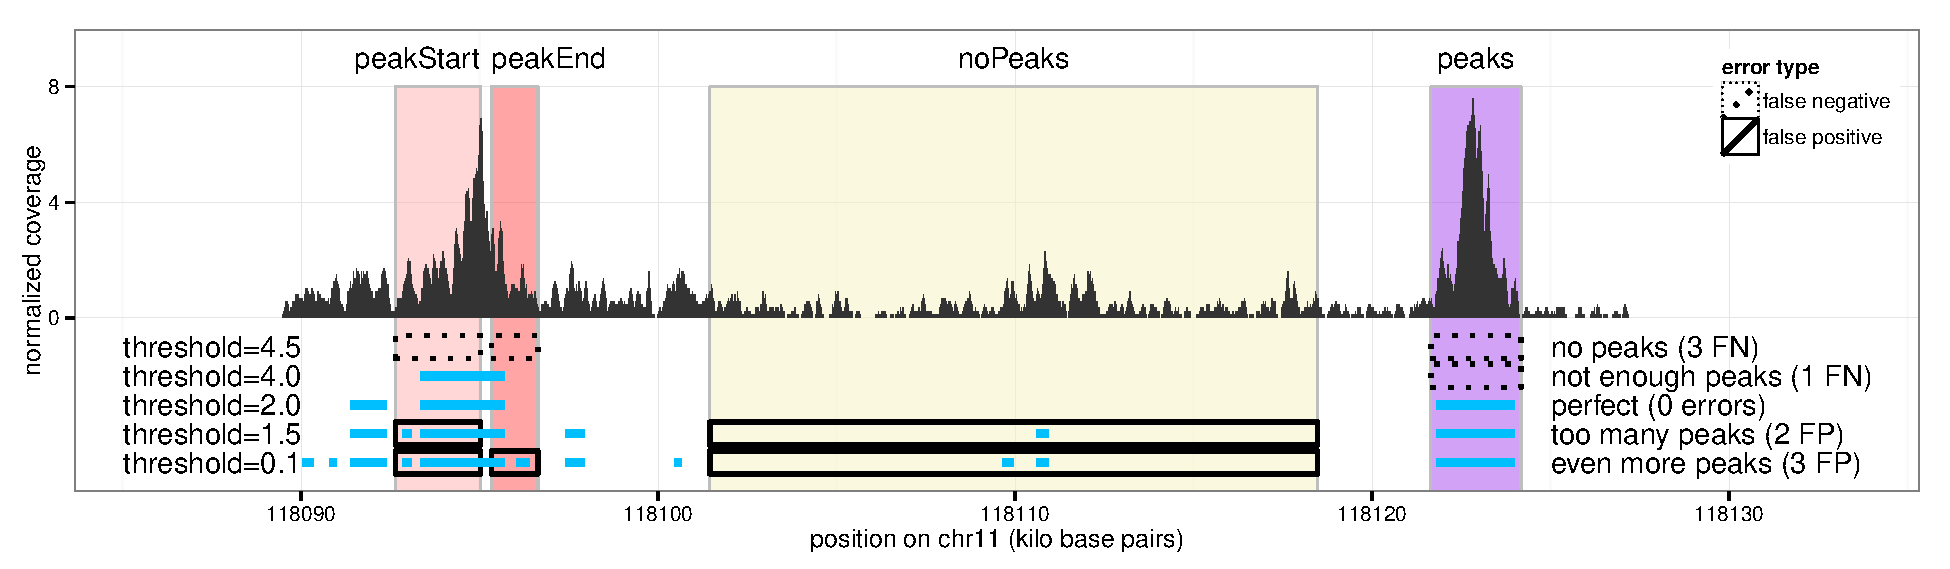
\includegraphics[width=\textwidth]{figure-PeakError.pdf}
  \begin{itemize}
  \item \textbf{peakStart}: exactly one peak start (0=FN, more=FP).
  \item \textbf{peakEnd}: exactly one peak end (0=FN, more=FP).
  \item \textbf{noPeaks}: no overlapping peaks (otherwise FP).
  \item \textbf{peaks}: at least one overlapping peak (otherwise FN).
  \item R package PeakError.
  \end{itemize}
\end{frame}

% \begin{frame}
%   \frametitle{Benchmark data sets, algorithms}

%  \url{http://cbio.ensmp.fr/~thocking/chip-seq-chunk-db/}
%   \begin{itemize}
%   \item Hocking \emph{et al} Bioinformatics (2016). Optimizing
%     ChIP-seq peak detectors using visual labels and supervised machine
%     learning.
%   \item 37 labeled H3K4me3 samples (sharp peak pattern).
%   \item 29 labeled H3K36me3 samples (broad peak pattern).
%   \item 12,826 labeled regions with and without peaks.
%   \item 2,752 separate segmentation problems.
%   \end{itemize}

%   Algorithms for $S$ optimal segmentations in $N$ data points:
%   \begin{center}
%   \begin{tabular}{ccccc}
%     algorithm & constraint & exact? & complexity \\
%     \hline
%     CDPA & $\mu_1 < \mu_2 > \mu_3 \dots$ & no & $O(S N^2)$\\
%     \textbf{GPDPA} &
%  $\mu_1 \leq \mu_2 \geq \mu_3 \dots$ & yes & $O(S N\log N)$ \\
%     PDPA & none & yes & $O(S N\log N)$
%   \end{tabular}

%   \vskip 0.5cm

%   PDPA loss $\leq$ GPDPA loss $\leq$ CDPA loss.
%   \end{center}
% \end{frame}
 
\begin{frame}
  \frametitle{Test AUC on 7 benchmark data sets}
  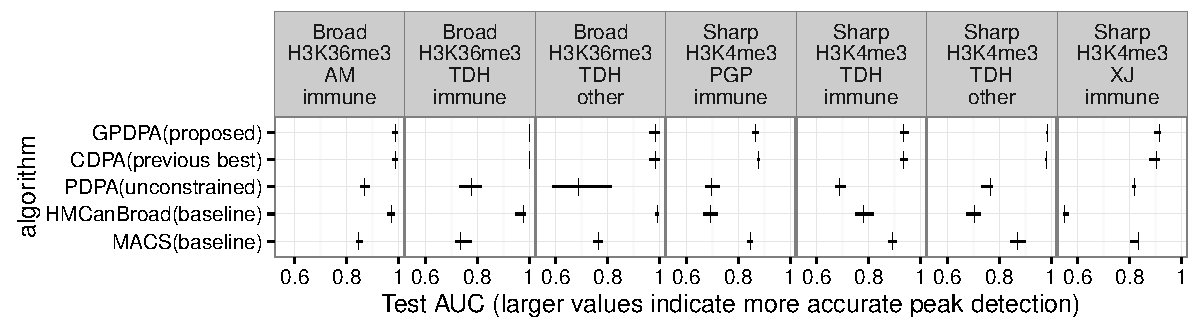
\includegraphics[width=\textwidth]{figure-test-error-dots}
  \begin{itemize}
  \item 4-fold cross-validation: train on 3/4 of labels, test on 1/4.
  \item All models trained by learning a scalar significance
    threshold / penalty parameter, which is varied to compute ROC/AUC.
  \item MACS is highly inaccurate in all data sets.
  \item HMCanBroad is accurate for broad but not sharp pattern.
  \item Unconstrained PDPA algorithm not as accurate as up-down
    constrained algorithms (CDPA, \textbf{proposed GPDPA}).
  \end{itemize}
  \scriptsize
\url{http://bl.ocks.org/tdhock/raw/886575874144c3b172ce6b7d7d770b9f/}
\end{frame}

\begin{frame}
  \frametitle{Functional pruning algorithms faster for larger data sets}
  %\includegraphics[width=1\textwidth]{figure-PDPA-timings.pdf}
  \input{figure-PDPA-timings-wide-labels}

  Total time to compute 10 models (0, ..., 9 peaks) for all problems:
  \begin{itemize}
  \item CDPA: 156 hours, inexact.
  \item GPDPA: 6 hours, exact.
  \end{itemize}
\end{frame}

\begin{frame}
  \frametitle{Contribution: new fast and exact constrained algorithm}
  \begin{tabular}{r|c|c}
    & no pruning & functional pruning \\
    \hline
    unconstrained & Dynamic Programming & Pruned DP \\
     & exact $O(S N^2)$ & exact $O(SN\log N)$\\
    R pkgs: & changepoint & cghseg, Segmentor\\
    \hline
    up-down constrained & constrained DP & \textbf{GPDPA} \\
     & inexact $O(SN^2)$ & exact $O(SN\log N)$\\
    R pkgs: & PeakSegDP & \textbf{PeakSegOptimal}\\
    \hline
  \end{tabular}
  \begin{itemize}
  \item New GPDPA that computes optimal changepoints 
    using the Poisson loss and the up-down constraint.
  \item State-of-the-art peak detection accuracy in ChIP-seq data.
  \item Empirically $O(S N \log N)$ time and memory for $N$ data
    points and $S$ segments.
  \item C++ code in PeakSegOptimal R package, 
    \url{https://cran.r-project.org/package=PeakSegOptimal}
  \end{itemize}
  Future work: other constraints and loss functions.
\end{frame}

\section{Other projects and future work}

\begin{frame}
  \frametitle{New labeling and training methods for breakpoint detection}

  H {\it et al.}, {\it BMC Bioinformatics} 2013.
  \begin{itemize}
  \item Create positive/breakpoint and negative/normal labels.
  \item Quantify/optimize error rate (number of incorrect labels).
  \item Benchmark data set of 3418 chromosomes,
    labeled via visual inspection (R package neuroblastoma).
  \item Results: most accurate model is maximum Gaussian likelihood 
    changepoint detection (cross-validation experiments).
  \end{itemize}

  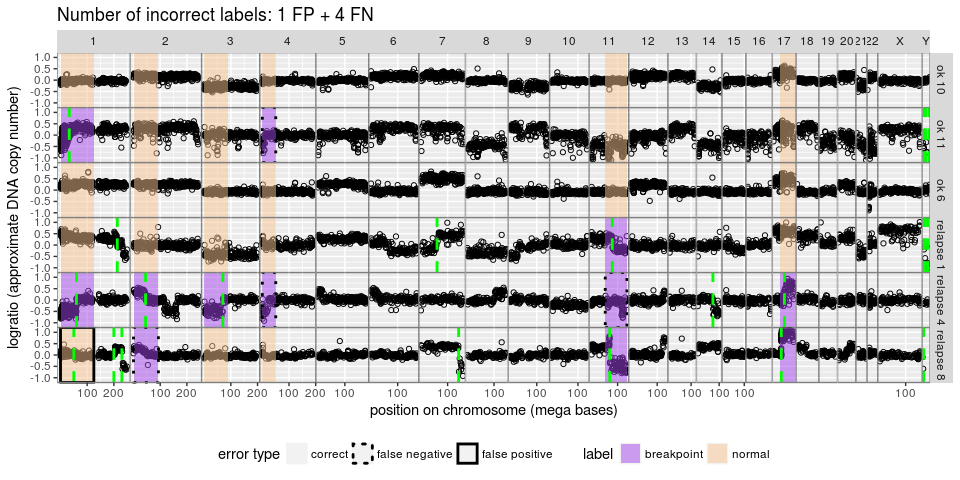
\includegraphics[width=\textwidth]{neuroblastoma-ok-relapse-supervised}

\end{frame} 

% \begin{frame}
%   \frametitle{Fast FPOP algorithm for computing the maximum likelihood
%     changepoint model}

%   Maidstone, Hocking, Rigaill, Fearnhead, {\it Stat. and
%     Comp.} 2017.

%   \begin{itemize}
%   \item Naively exponential $O(p^K)$ time to compute best model with
%     $K$ segments ($K-1$ changes) for a sequence of $p$ data.
%   \item Previous work: other algorithms for computing the model
%     (\algo{PELT} and \algo{pDPA}).
%   \item Contribution: new log-linear $O(p\log p)$ \algo{FPOP}
%     algorithm for computing the same model (R package fpop).
%   \end{itemize}
%   \begin{center}
%     \includegraphics[width=0.5\textwidth]{figure-systemtime-arrays-bins}
%   \end{center}
% \end{frame}

\begin{frame}
  \frametitle{Supervised interactive DNA copy number analysis}
  H {\it et al.}, {\it Bioinformatics} 2014.

  \begin{itemize}
  \item Previous work: non-interactive command line programs
    -- collaborators can not correct obvious
    errors.
  \item Interactive system: when you edit the labels, the system
    learns and updates the model. (SegAnnDB python module)
  \item Result below: only a few labels required to learn a highly accurate
    breakpoint detection model.
  \end{itemize}
  \begin{minipage}{0.5\linewidth}
    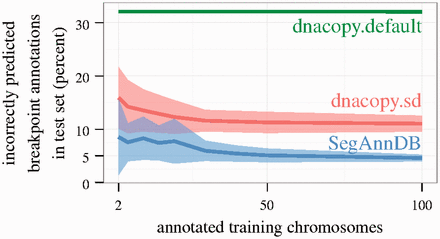
\includegraphics[width=\textwidth]{SegAnnDB-test-error-decreases}
  \end{minipage}
  \begin{minipage}[0.5\linewidth]{0.48\linewidth}
SegAnnDB demo:\\interactively label chr1/chrX
  \url{http://bioviz.rocq.inria.fr/profile/GSM313887/}
  \end{minipage}
\end{frame}

\begin{frame}
  \frametitle{Cancer biology applications}
  Aichi cancer center, Nagoya, Japan.
  \begin{itemize}
  \item Suguro {\it et al.}, {\it Cancer Sci} 2014, Clonal
    heterogeneity of lymphoid malignancies correlates with poor
    prognosis.
  \item Shimada {\it et al.}, {\it Leukemia} 2016, Development and
    analysis of patient-derived xenograft mouse models in
    intravascular large B-cell lymphoma.
  \end{itemize}
  Institut Curie, Paris, France.
  \begin{itemize}
  \item Chicard {\it et al.}, {\it Clinical Cancer Research} 2016,
    Genomic copy number profiling using circulating free tumor DNA
    highlights heterogeneity in neuroblastoma.
  \item Ongoing work, characterizing alterations in neuroblastoma.
  \end{itemize}
\end{frame}

\begin{frame}
  \frametitle{Other research projects}
  \begin{tabular}{ll}
Unsupervised convex & \multirow{4}{*}{
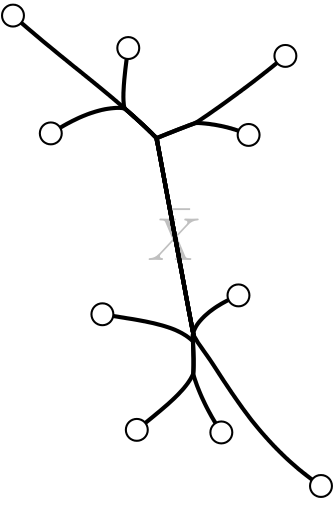
\includegraphics[height=0.2\textheight]{screenshot-clusterpath}
}\\
hierarchical clustering.\\
H {\it et al.}, {\it ICML} 2011\\
%91 citations. 
R package clusterpath. \\
\hline
Predicting the  & \multirow{4}{*}{
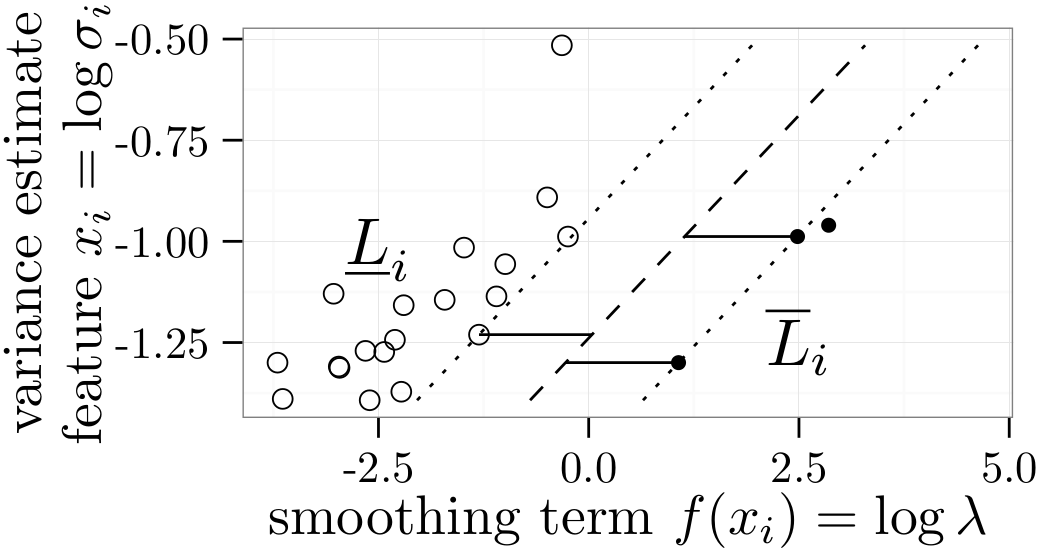
\includegraphics[height=0.25\textheight]{Screenshot-max-margin}
}\\
number of changepoints.\\
H {\it et al.}, {\it ICML} 2013. \\
R package penaltyLearning.\\
useR2017 tutorial.\\
\hline
Support vector machines & \multirow{4}{*}{ 
    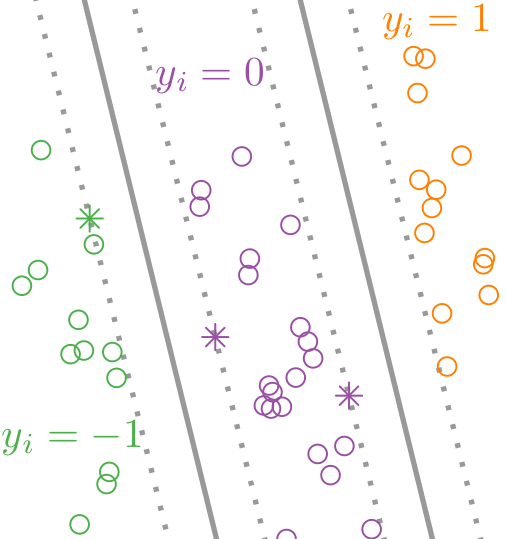
\includegraphics[height=0.2\textheight]{screenshot-ranksvmcompare}
}\\
for ranking and comparison. \\
H {\it et al.}, arXiv:1401.8008. \\
R package rankSVMcompare.\\
\hline
New interactive keywords& \multirow{5}{*}{
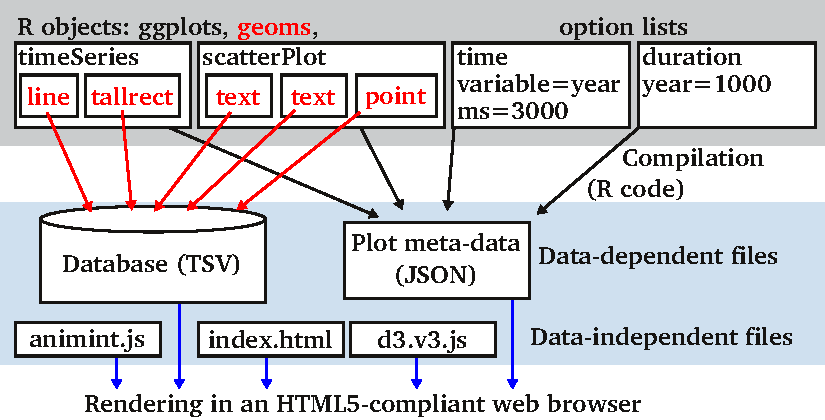
\includegraphics[height=0.2\textheight]{figure-design}
}\\
for the grammar of graphics,\\
under review at \emph{Journal}\\
\emph{of Computational and Graphical}\\
\emph{Statistics}, R package animint.\\
%useR2016 tutorial.\\
  \end{tabular}
  % \begin{minipage}{0.3\linewidth}
  %   Clusterpath for convex hierarchical clustering (H {\it et
  %     al.}, {\it ICML} 2011, 91 citations). R package clusterpath.
  %   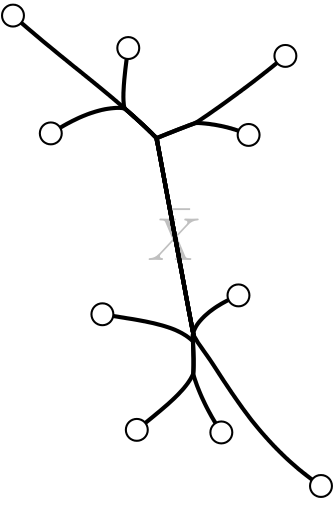
\includegraphics[width=\linewidth]{screenshot-clusterpath}
  % \end{minipage}
  % \begin{minipage}{0.3\linewidth}
  %   Support vector machines for ranking and comparison. H {\it et
  %     al.}, arXiv:1401.8008. R package rankSVMcompare.
  %   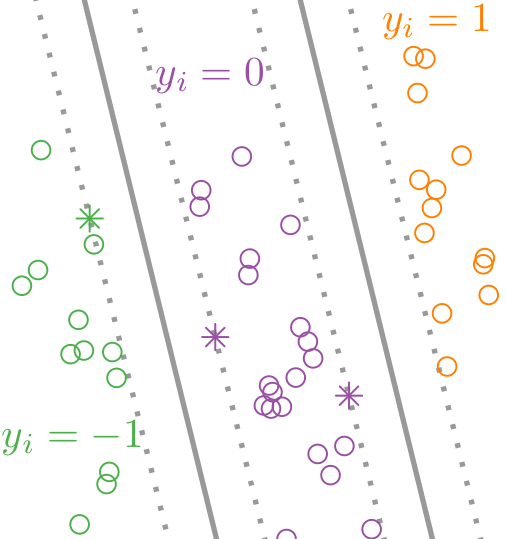
\includegraphics[width=\linewidth]{screenshot-ranksvmcompare}
  % \end{minipage}
  % \begin{minipage}{0.3\linewidth}
  %   New interactive keywords for the grammar of graphics, under review
  %   at \emph{Journal of Computational and Graphical Statistics}, R
  %   package animint.
  % \end{minipage}

  % Collaborations at the McGill Genome Center:
  % \begin{itemize}
  % \item Predicting which people will respond to the flu vaccine based
  %   on SNP data. (with Maiko Narahara)
  % \item Predicting which people have asthma based on SNP
  %   data. (with Audrey Grant)
  % \item Predicting which genetic variants are pathogenic based on
  %   biochemistry, evolutionary conservation, etc. (with
  %   Najmeh Alirezaie)
  % % \item Predicting genomic regions with peaks based on ChIP-seq
  % %   data. (with Guillaume Bourque)
  % \end{itemize}
\end{frame}
 
\begin{frame}
  \frametitle{Future projects for my research lab}
  \begin{itemize}
  %\item Collaborations with experts from other scientific domains.
  % \item Supervising graduate students who want to work on algorithms
  %   for solving important big data analysis problems.
  \item Multi-task learning for predicting the number of changepoints
    (multiple scientists provide breakpoint or peak labels).
  % \item Survival models for predicting the number of changepoints: R
  %   package iregnet.
  \item Fast algorithms for other constrained changepoint models
    (neuro spike train data, segmented regression, etc).
  \item Deep learning for nonparametric changepoint detection.
  \item GenomicLearner platform for collaborations: interactive
    labeling and machine learning analysis.
  \end{itemize}
\end{frame}


% \begin{frame}[fragile]
%   \frametitle{How to choose parameters of unsupervised peak
%     detectors?}
% \scriptsize
% 19 parameters for Model-based analysis of ChIP-Seq (MACS), Zhang et al, 2008.
% \begin{verbatim}
%   [-g GSIZE]
%   [-s TSIZE] [--bw BW] [-m MFOLD MFOLD] [--fix-bimodal]
%   [--nomodel] [--extsize EXTSIZE | --shiftsize SHIFTSIZE]
%   [-q QVALUE | -p PVALUE | -F FOLDENRICHMENT] [--to-large]
%   [--down-sample] [--seed SEED] [--nolambda]
%   [--slocal SMALLLOCAL] [--llocal LARGELOCAL]
%   [--shift-control] [--half-ext] [--broad]
%   [--broad-cutoff BROADCUTOFF] [--call-summits]
% \end{verbatim}
% 10 parameters for Histone modifications in cancer (HMCan),
% Ashoor et al, 2013.
% \begin{verbatim}
% minLength 145
% medLength 150
% maxLength 155
% smallBinLength 50
% largeBinLength 100000
% pvalueThreshold 0.01
% mergeDistance 200
% iterationThreshold 5
% finalThreshold 0
% maxIter 20
% \end{verbatim}
% \end{frame}

% \begin{frame}
%   \frametitle{PeakSeg: search for the peaks with lowest loss}
%   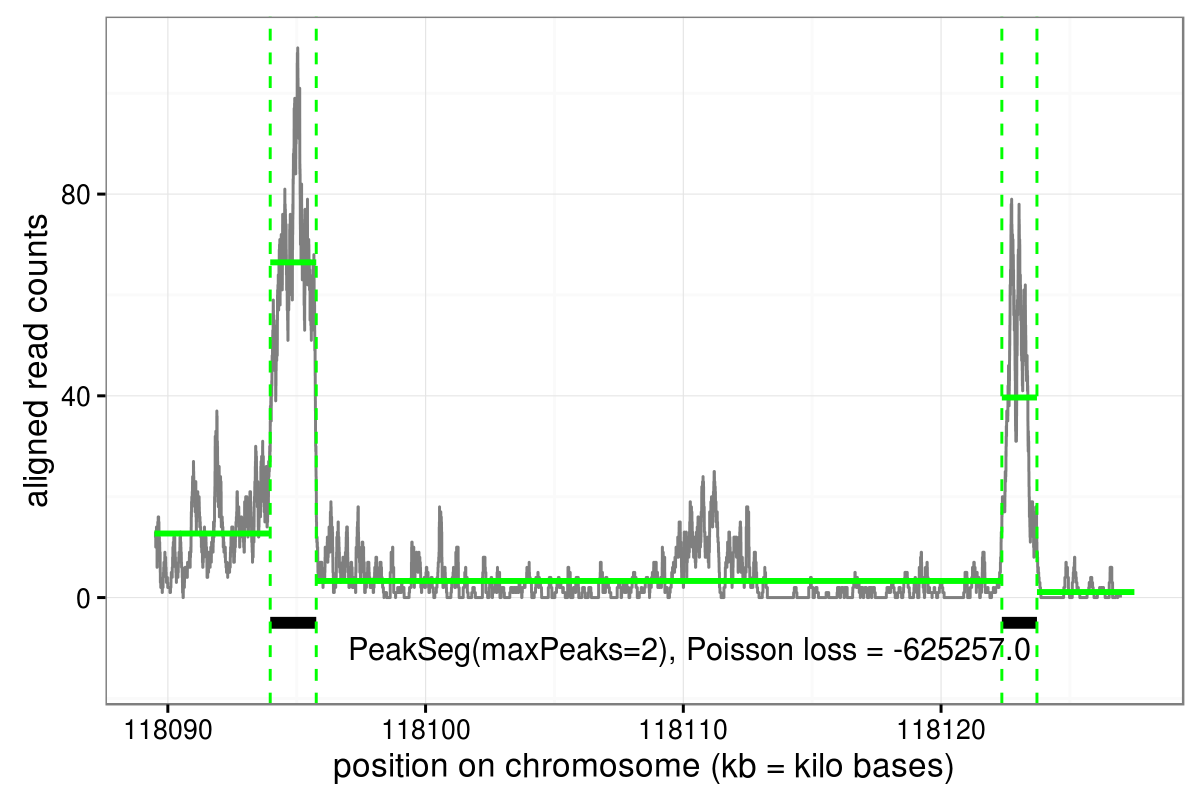
\includegraphics[width=1\textwidth]{figure-macs-problem-PeakSeg.png}
  
%   Simple model with only one parameter (number of peaks).\\
%   But computationally difficult!
% \end{frame}

\begin{frame}
  \frametitle{Thanks for your attention!}

  Questions? toby.hocking@mail.mcgill.ca
  \begin{itemize}
  \item A log-linear time algorithm for constrained changepoint
    detection, by Toby Dylan Hocking, Guillem Rigaill, Paul Fearnhead,
    Guillaume Bourque \url{https://arxiv.org/abs/1703.03352}
  \item 
  PeakSegOptimal R package, \\
\url{https://cran.r-project.org/package=PeakSegOptimal}
  \item source code for these slides:
  \url{https://github.com/tdhock/PeakSegFPOP-paper}
  \end{itemize}
\end{frame}

\section*{Results on comparing several samples}

\begin{frame}
  \frametitle{Target interval computation time}
  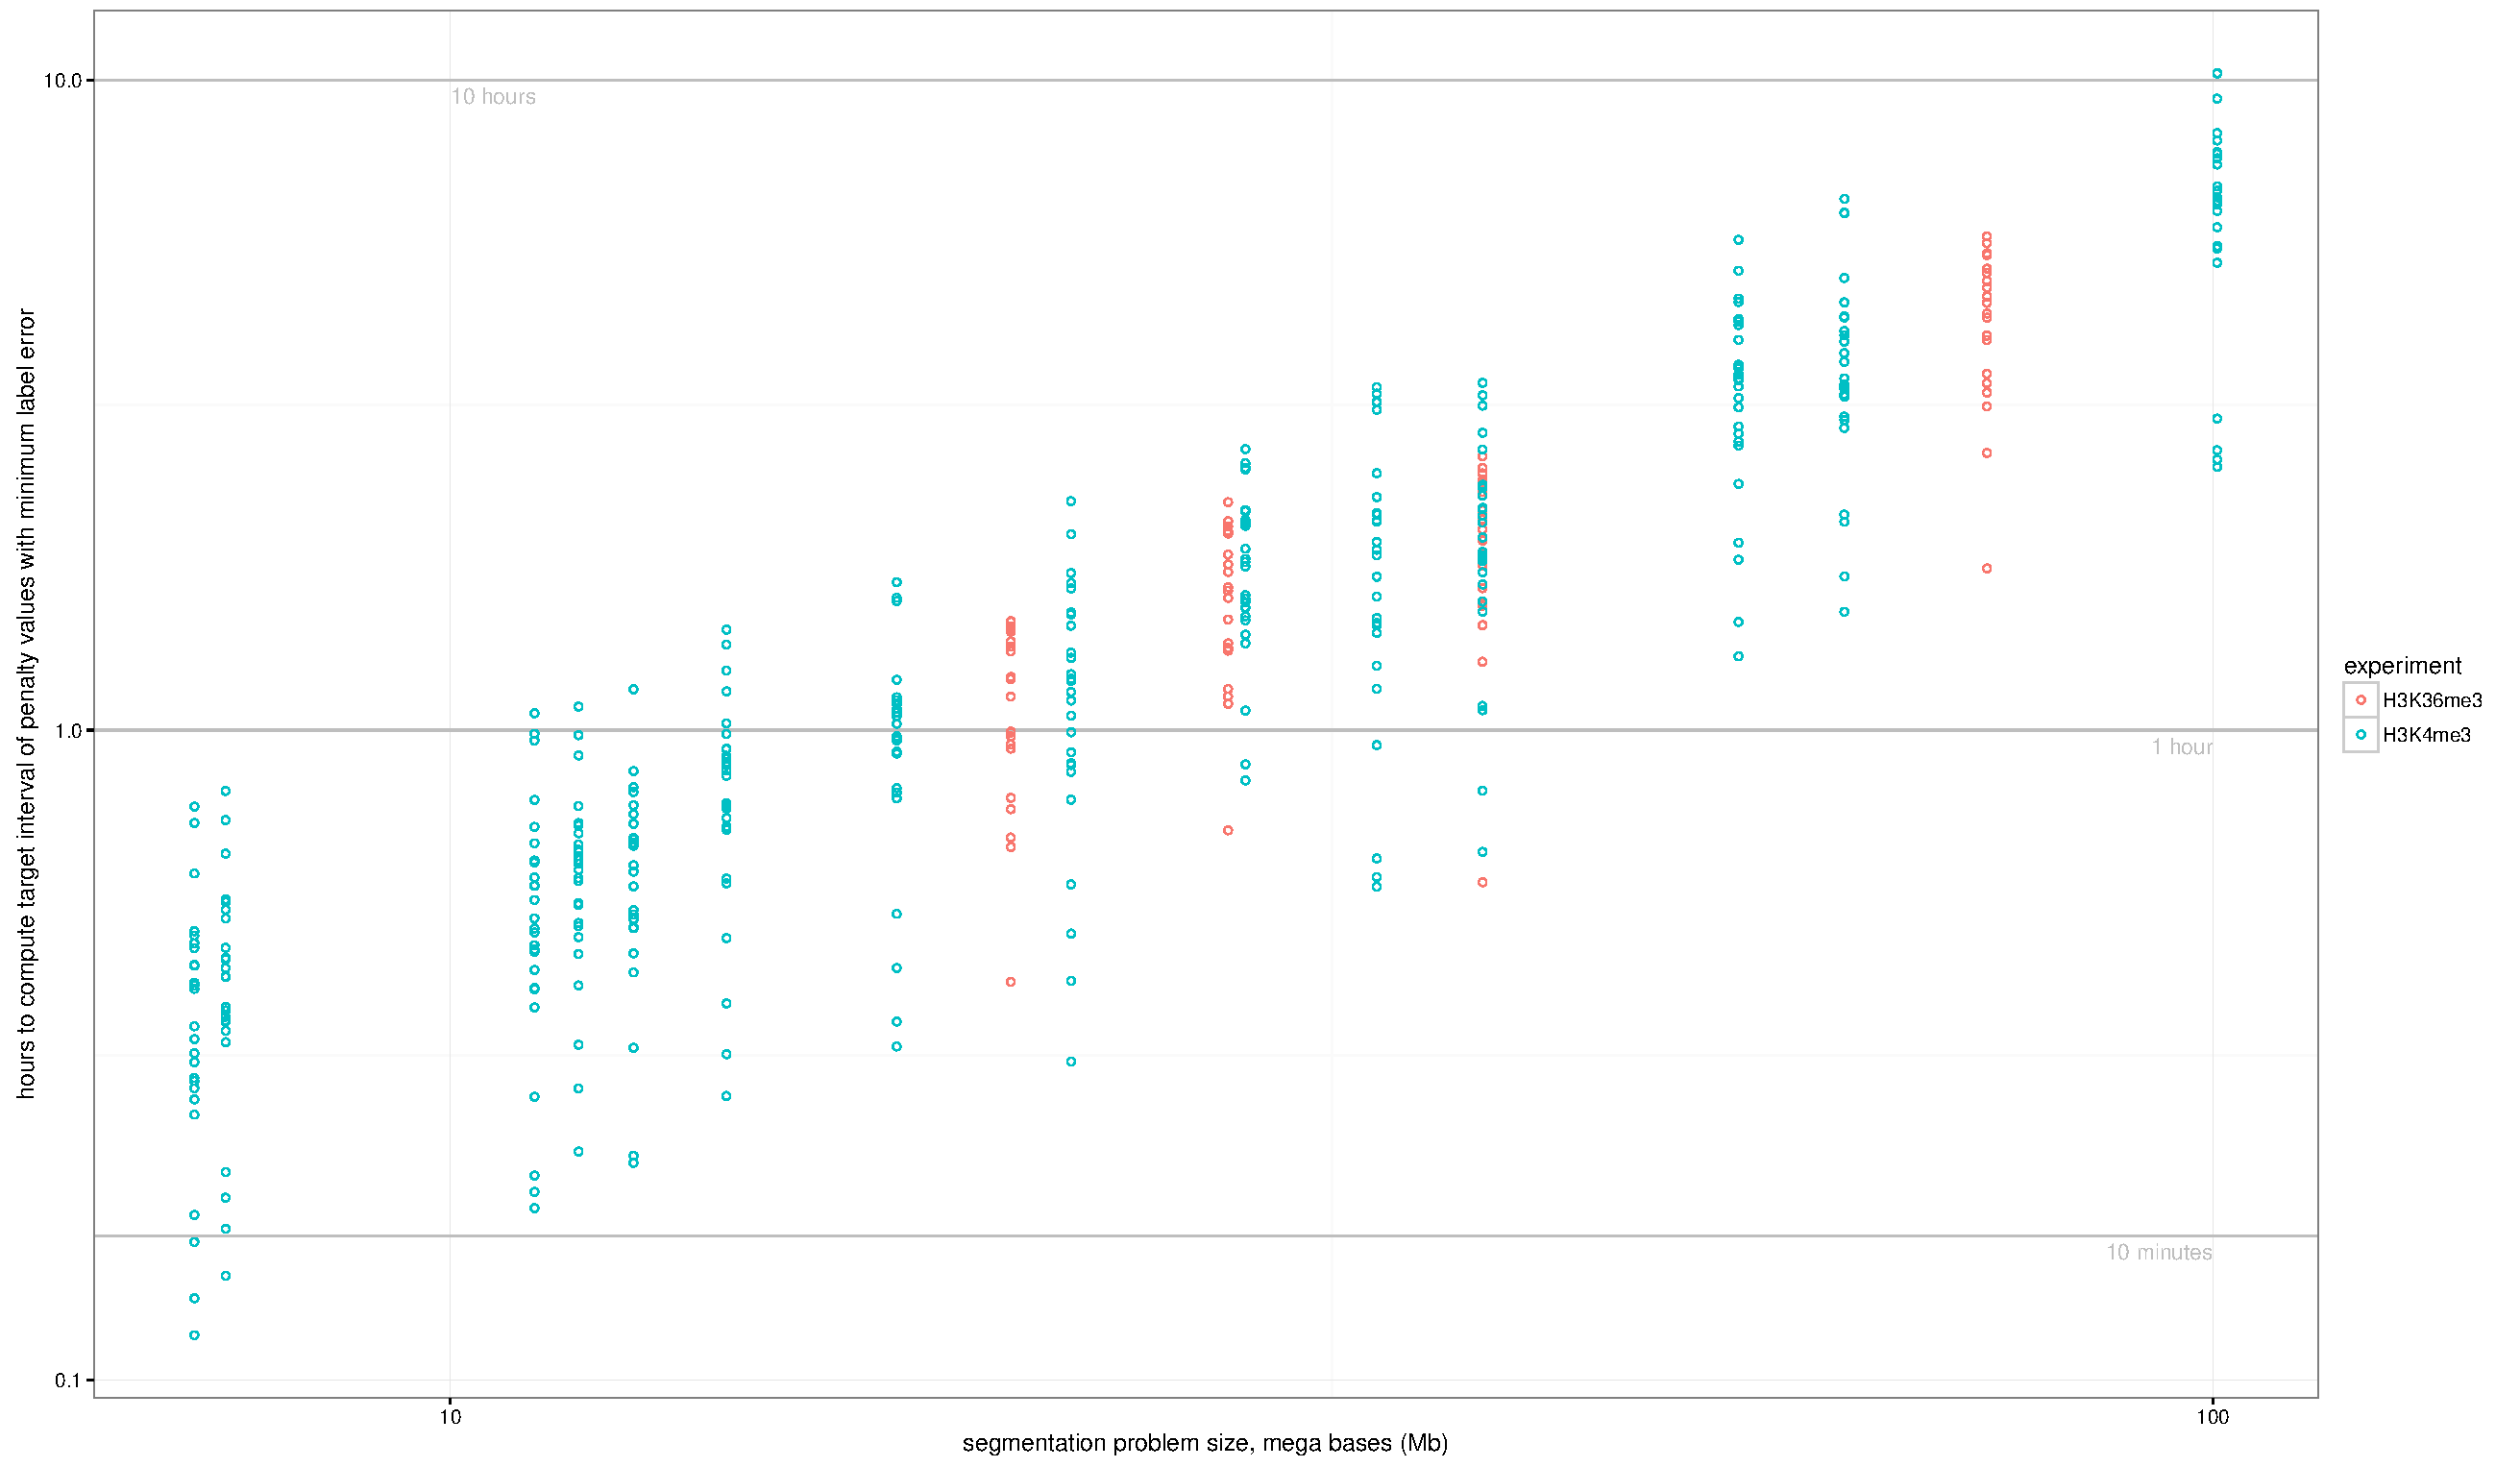
\includegraphics[width=\textwidth]{figure-target-interval-time}
\end{frame}

\begin{frame}
  \frametitle{More peaks in sharp H3K4me3 than in broad H3K36me3}
  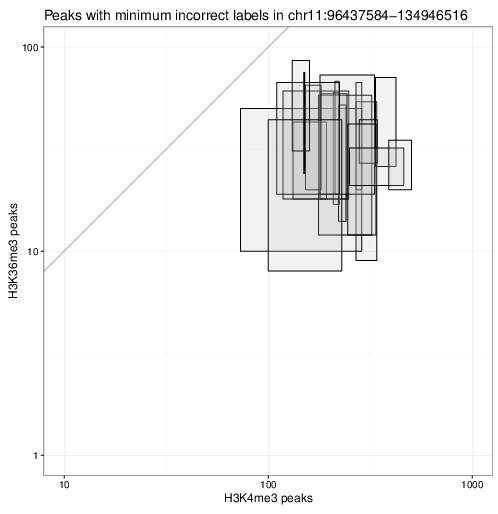
\includegraphics[width=0.7\textwidth]{figure-min-err-peaks-compare}
\end{frame}

\begin{frame}
  \frametitle{More peaks in sharp H3K4me3 than in broad H3K36me3}
  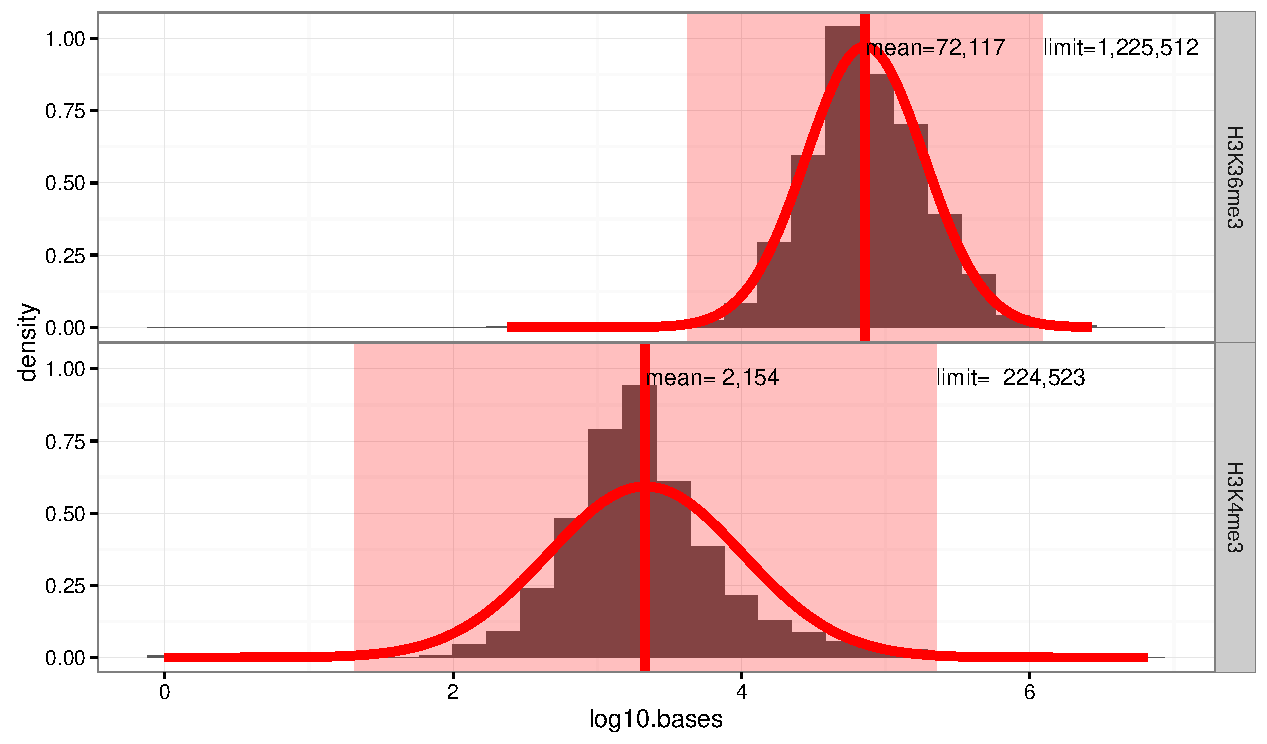
\includegraphics[width=0.7\textwidth]{figure-peak-size-model}
\end{frame}

\begin{frame}
  \frametitle{Max-margin penalty learning algortihm}
  \includegraphics[width=\textwidth]{figure-large-margin}
 
\scriptsize \url{http://bl.ocks.org/tdhock/raw/9311ca39d643d127e04a088814c81ee1/}

\end{frame}

% \begin{frame}
%   \frametitle{Segmenting whole chromosomes?}
%   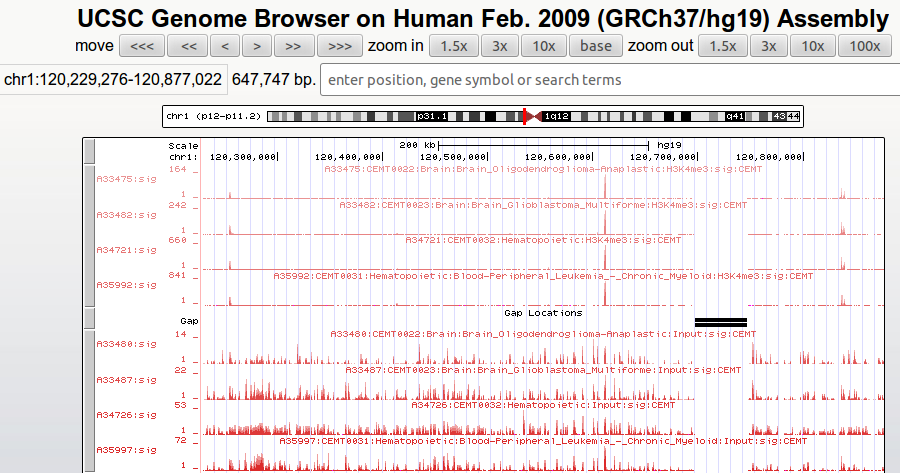
\includegraphics[width=\textwidth]{screenshot-gap-peaks}
%   \begin{itemize}
%   \item 365 regions with no gaps in hg19.
%   \item 272 regions with no gaps on chr1-22, X, Y.
%   \item Smallest: 31,833 bases (chr6:157,609,467-157,641,300).
%   \item Largest: 115,591,997 bases (chr4:75,452,279-191,044,276).
%   \end{itemize}
% \end{frame}


% \begin{frame}
%   \frametitle{Reasonable time to segment biggest region on chr1}
%   \includegraphics[width=\textwidth]{figure-cosegData-timings.pdf}
%   \begin{itemize}
%   \item R package in memory: $O(N \log N)$ time.
%   \item Command line program on disk: $O(N \log N)$ time.
%   \end{itemize}
% \end{frame}

% \begin{frame}
%   \frametitle{Memory requirements reasonable for on-disk version}
%   \includegraphics[width=\textwidth]{figure-cosegData-timings-memory-disk.pdf}
%   \begin{itemize}
%   \item R package in memory: $O(N \log N)$ memory.
%   \item Command line program on disk: $O(\log N)$ memory.
%   \end{itemize}
% \end{frame}

% \begin{frame}
%   \frametitle{Disk usage reasonable}
%   \includegraphics[width=\textwidth]{figure-cosegData-timings-disk.pdf}
%   \begin{itemize}
%   \item R package in memory: no disk usage.
%   \item Command line program: $O(N \log N)$ disk space (temporary).
%   \end{itemize}
% \end{frame}

\begin{frame}
  \frametitle{Two annotators provide consistent labels, but different
    precision}
  \includegraphics[width=1.1\textwidth]{../chip-seq-paper/screenshot-several-annotators}

  \begin{itemize}
  \item TDH peakStart/peakEnd more precise than AM peaks.
  \item AM noPeaks more precise than TDH no label.
  \end{itemize}
\end{frame}

\begin{frame}
  \frametitle{Train on one person, test on another\\
(same histone mark and samples)}
  \includegraphics[width=1\textwidth]{../chip-seq-paper/figure-splits-H3K4me3-annotators.pdf}
\end{frame}

\begin{frame}
  \frametitle{Train on one person, test on another\\
(same histone mark and samples)}
  \includegraphics[width=1.1\textwidth]{../chip-seq-paper/figure-test-H3K4me3-annotators.pdf}
\end{frame}

\begin{frame}
  \frametitle{Train on some samples, test on others\\
(same histone mark and person)}
  \includegraphics[width=1\textwidth]{../chip-seq-paper/figure-splits-H3K4me3-types.pdf}
\end{frame}

\begin{frame}
  \frametitle{Train on some samples, test on others\\
(same histone mark and person)}
  \includegraphics[width=1.1\textwidth]{../chip-seq-paper/figure-test-H3K4me3-types.pdf}
\end{frame}

\begin{frame}
  \frametitle{Train on one histone mark, test on another\\
(same person and samples)}
  \includegraphics[width=1\textwidth]{../chip-seq-paper/figure-splits-TDH-experiments.pdf}
\end{frame}

\begin{frame}
  \frametitle{Train on one histone mark, test on another\\
(same person and samples)}
  \includegraphics[width=1.1\textwidth]{../chip-seq-paper/figure-test-TDH-experiments.pdf}
\end{frame}


\begin{frame}
  \frametitle{PeakSeg with 2 peaks more likely than default macs}
  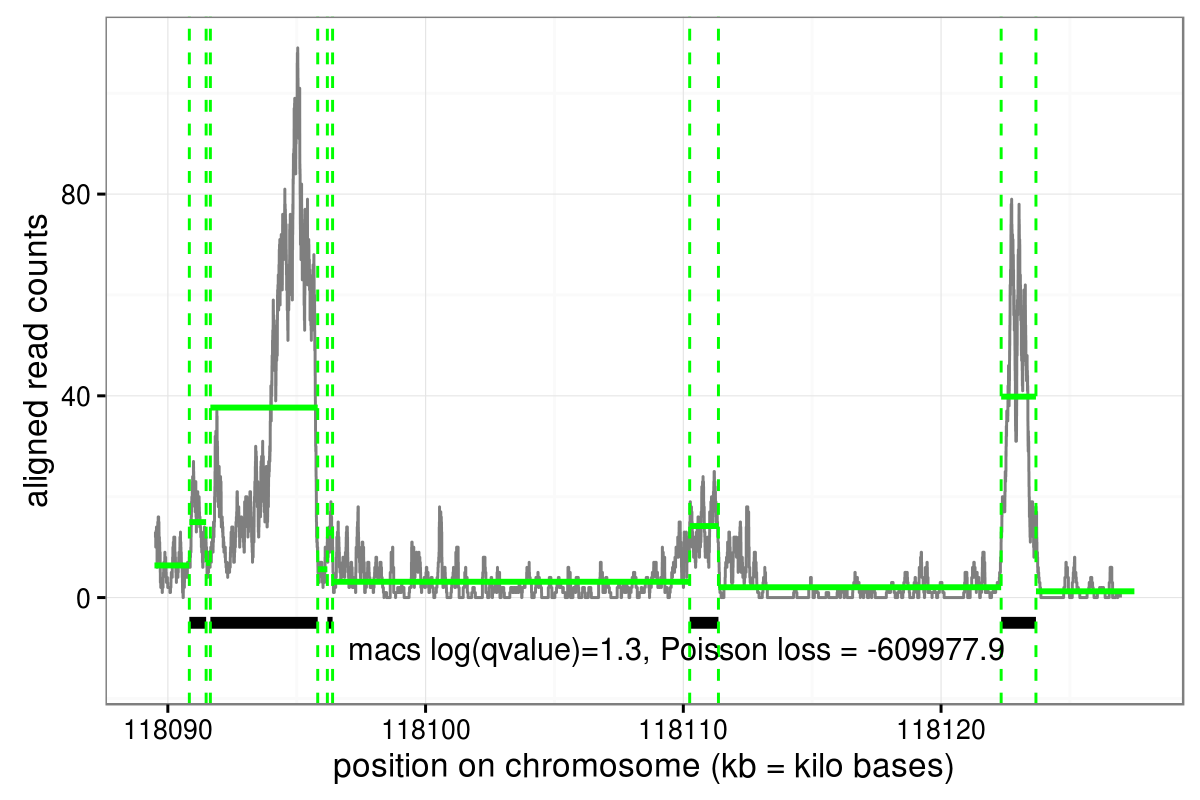
\includegraphics[width=1\textwidth]{figure-macs-problem-1-30103.png}
\end{frame}

\begin{frame}
  \frametitle{Unconstrained model can have any changes}
  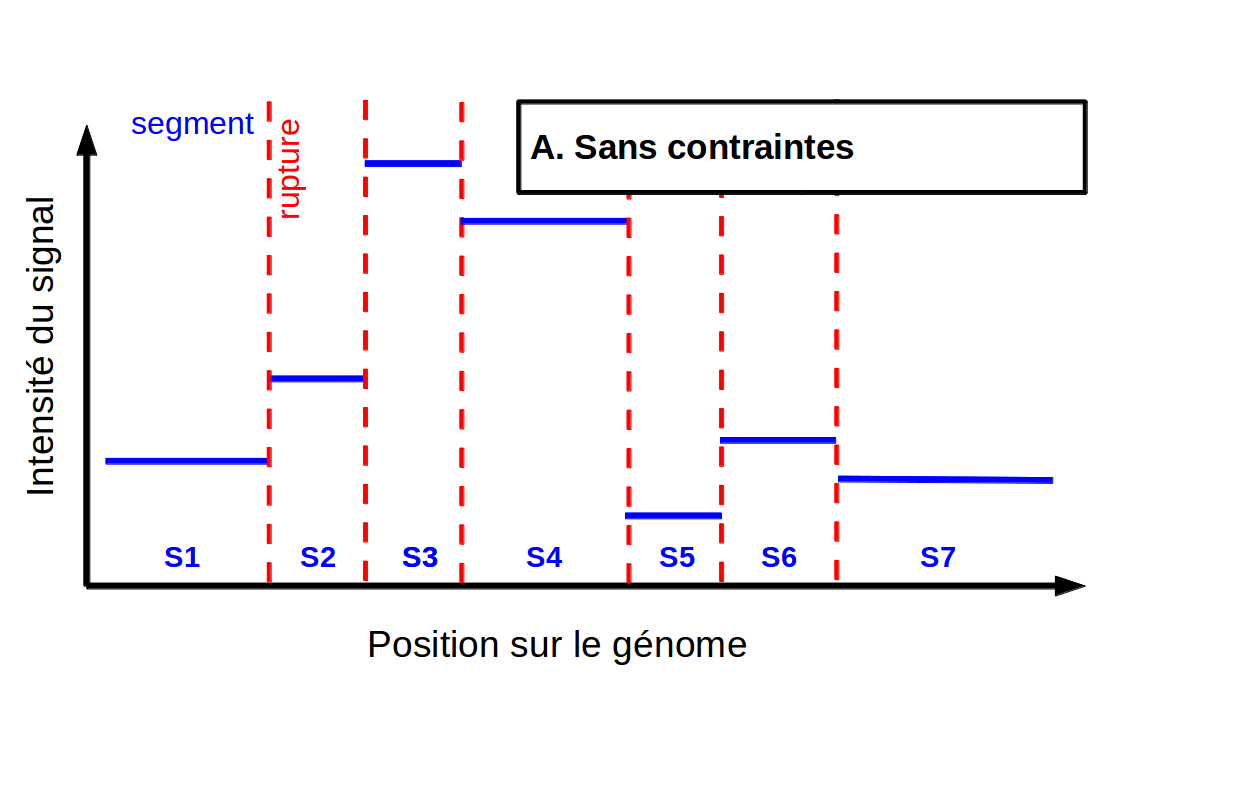
\includegraphics[width=1\textwidth]{Seg_SansC.png}
  \vskip -1cm
  \begin{itemize}
  \item The model above does NOT verify the PeakSeg up-down constraint
    (second change is up, should be down).
  \item Not directly interpretable as background and peaks.
  \end{itemize}
\end{frame}

\begin{frame}
  \frametitle{PeakSeg constraint forces up then down changes}
  \includegraphics[width=1\textwidth]{Seg_AvecC1.png}
  \vskip -1cm
  \begin{itemize}
  \item Novelty of PeakSeg model with respect to previous optimal
    segmentation models: the up-down constraint.
  \item Interpretable as background (S1, S3, ...)\\
    and peaks (S2, S4, ...).
  \end{itemize}
\end{frame}

\section*{Interpretation of equal segment means}

\begin{frame}
  \frametitle{What does our solution say about the PeakSeg solution?}
  \begin{itemize}
  \item Our algo exactly solves a problem with \textbf{non-strict
      inequality} constraints.
  \item For example, $N=3$ data points and $S=3$ segments,
    \begin{equation*}
      \min_{m_1\leq m_2\geq m_3}
      \sum_{t=1}^N m_t - z_t\log m_t.
    \end{equation*}
  \item But the PeakSeg problem has \textbf{strict inequality}
    constraints:
    \begin{equation*}
      \min_{m_1<m_2 >m_3}
      \sum_{t=1}^N m_t - z_t\log m_t.
    \end{equation*}
  \end{itemize}
  When our algo returns equal values for adjacent segment means,
  \begin{itemize}
  \item Our solution is not feasible for the PeakSeg problem, and
  \item The PeakSeg solution is undefined.
  \end{itemize}
\end{frame}


\begin{frame}
  \frametitle{Example: 13, 14, 10, 1}
  What do you think is the best model with 1 peak?\\
  (3 segments, 1 change up, 1 change down)
  
  \vskip 1cm

  Guessing game:

  \url{https://github.com/tdhock/PeakSegFPOP-paper/blob/master/figure-min-undefined.R} 
\end{frame}

\begin{frame}
  \frametitle{PeakSegDP returns this highly suboptimal model}
  \includegraphics[width=\textwidth]{figure-min-undefined-suboptimal}
\end{frame}

\begin{frame}
  \frametitle{A better model}
  \includegraphics[width=\textwidth]{figure-min-undefined-1}
\end{frame}

\begin{frame}
  \frametitle{Even better}
  \includegraphics[width=\textwidth]{figure-min-undefined-2}
\end{frame}

\begin{frame}
  \frametitle{Still better}
  \includegraphics[width=\textwidth]{figure-min-undefined-3}
\end{frame}

\begin{frame}
  \frametitle{We can keep going forever}
  \includegraphics[width=\textwidth]{figure-min-undefined-4}
\end{frame}

\begin{frame}
  \frametitle{Best model is not feasible}
  \includegraphics[width=\textwidth]{figure-min-undefined}
\end{frame}
 
\section*{Segmentation problem definitions}

\begin{frame}
  \frametitle{Unconstrained maximum likelihood segmentation}
  \begin{itemize}
  \item We have a sequence of $n$ count data $\mathbf y\in\ZZ_+^n$ to
    segment. 
  \item Choose the number of segments $S\in\{1, 2, \dots, n\}$.
  \end{itemize}
\begin{align*}
  \minimize_{\substack{
  \mathbf m\in\RR^{n}
\\
  \mathbf c\in\{-1,0,1\}^{n-1}
  }} &\ \ 
    \sum_{t=1}^n \ell( m_t,  z_t) 
\\
    \text{subject to} &\ \  1+\sum_{t=1}^{n-1} I(c_t \neq 0) = S, 
\nonumber\\
& \ \ c_t = -1 \Rightarrow m_{t} > m_{t+1} \text{ (change down)}
\nonumber\\
& \ \ c_t = 0 \Rightarrow m_{t} = m_{t+1}  \text{ (no change)}
\nonumber\\
& \ \ c_t = 1 \Rightarrow m_{t} < m_{t+1} \text{ (change up)}
\nonumber
\end{align*}
\begin{itemize}
\item The Poisson loss function is  $\ell( m,  y)= m - y \log m$.
\item Every $t$ such that $c_t \neq 0$ is a
change-point.
\end{itemize}

\end{frame}

% We refer to (\ref{unconstrained}) as the ``unconstrained'' model
% since $\mathbf{\hat m}^K(\mathbf y)$ is the most likely segmentation
% of all possible models with $K$ piecewise constant segments ($K-1$
% change-points). 
% Although (\ref{unconstrained}) is a non-convex optimization problem,
% the sequence of segmentations
% $\mathbf{\hat m}^1(\mathbf y), \dots, \mathbf{\hat m}^{K}(\mathbf y)$
% can be computed in $O(K n^2)$ time using the standard dynamic
% programming algorithm \citep{bellman}, or in $O(K n \log n)$ time
% using dynamic programming with functional pruning \citep{pruned-dp,
%   johnson, Segmentor}.

\begin{frame}
  \frametitle{The PeakSeg constrained maximum likelihood model}
\begin{align*}
    \minimize_{\substack{
  \mathbf m\in\RR^{n}
\\
  \mathbf c\in\{-1,0,1\}^{n-1}
  }} &\ \ 
    \sum_{t=1}^n \ell( m_t,  z_t) \\
    \text{subject to} &\ \  1+\sum_{t=1}^{n-1} I(c_t \neq 0) = S, \\
& \ \ c_t = -1 \Rightarrow m_{t} > m_{t+1} \text{ (change down)}\\
& \ \ c_t = 0 \Rightarrow m_{t} = m_{t+1}  \text{ (no change)}\\
& \ \ c_t = 1 \Rightarrow m_{t} < m_{t+1} \text{ (change up)}\\
&\ \ \forall t\in\{1, \dots, n-1\},\, \alert{P_t(\mathbf c) \in\{0, 1\}}.
\end{align*}
The only difference with the unconstrained problem is that\\
\alert{we
have added the constraint $P_t(\mathbf c)=\sum_{i=1}^t c_i \in\{0, 1\}$}.
% Another way to interpret the constrained
% \ref{PeakSeg} problem is that the sequence of changes in the segment
% means $\mathbf m$ must begin with a positive change and then
% alternate: up, down, up, down, ... (and not up, up, down). Thus the
% even-numbered segments may be interpreted as peaks $P_t(\mathbf c)=1$,
% and the odd-numbered segments may be interpreted as background
% $P_t(\mathbf c)=0$.
\end{frame}

\begin{frame}
  \frametitle{The problem solved by the PeakSegPDPA}
\begin{align*}
    \minimize_{\substack{
  \mathbf m\in\RR^{n}
\\
  \mathbf c\in\{-1,0,1\}^{n-1}
  }} &\ \ 
    \sum_{t=1}^n \ell( m_t,  z_t) 
  \label{PeakSegPDPA}
\\
    \text{subject to} &\ \  1+ \sum_{t=1}^{n-1} I(c_t \neq 0) = S, 
\nonumber\\
& \ \ c_t = -1 \Rightarrow m_{t} \alert{\geq} m_{t+1} \text{ (change down or no change)}
\nonumber\\
& \ \ c_t = 0 \Rightarrow m_{t} = m_{t+1}  \text{ (no change)}
\nonumber\\
& \ \ c_t = 1 \Rightarrow m_{t} \alert{\leq} m_{t+1} \text{ (change up or no change)}
\nonumber\\
&\ \ \forall t\in\{1, \dots, n-1\},\, P_t(\mathbf c) \in\{0, 1\}.
\nonumber
\end{align*}
\begin{itemize}
\item The only difference with the \textbf{PeakSeg} problem is that\\
  \alert{we have changed the strict inequality constraints to non-strict inequality
constraints}. 
\item This model has \textbf{at most} $S$ distinct
  segment means (some may be equal due to the non-strict equality
  constraints).
\end{itemize}
\end{frame}


% \section*{Review of constrained dynamic programming algorithm}

% \input{figure-dp-first}

% \input{figure-dp-short}

% \input{figure-dp}

% \begin{frame}
%   \frametitle{Dynamic programming is faster than grid search for $s>
%     2$ segments}

%   Computation time in number of data points $N$:

%   \vskip 1cm

%   \begin{tabular}{ccc}
%     segments $s$ & grid search & dynamic programming \\
%     \hline
%     1 & $O(N)$ & $O(N)$ \\
%     2 & $O(N^2)$ & $O(N^2)$ \\
%     3 & $O(N^3)$ & $O(N^2)$ \\
%     4 & $O(N^4)$ & $O(N^2)$ \\
%     $\vdots$ &     $\vdots$ &     $\vdots$ 
%   \end{tabular}

%   \vskip 1cm

%   For example $N = 5735$ data points to segment.\\
%   $N^2 = 32890225$\\
%   $N^3 = 188625440375$\\
%   $\vdots$
% \end{frame}

% \input{figure-dp-third}

% \begin{frame}
%   \frametitle{5 errors for coseg/Segmentor, only 1 error for PeakSegDP}
%   \includegraphics[width=\textwidth]{figure-min-train-error-problem1}
% \end{frame}

% \begin{frame}
%   \frametitle{5 errors for coseg/Segmentor, only 1 error for PeakSegDP}
%   \includegraphics[width=\textwidth]{figure-min-train-error-problem1-best.png}
% \end{frame}

% \begin{frame}
%   \frametitle{Constrained optimization worse than macs}
%   \includegraphics[width=\textwidth]{figure-min-train-error-problem4}
% \end{frame}

% \begin{frame}
%   \frametitle{Constrained optimization worse than macs}
%   \includegraphics[width=\textwidth]{figure-min-train-error-problem4-best}
% \end{frame}

% \begin{frame}
%   \frametitle{Constrained optimization worse than macs}
%   \includegraphics[width=\textwidth]{figure-min-train-error-problem4-best-zoom}
% \end{frame}


% \begin{frame}
%   \frametitle{Functional pruning complete example}
% %\includegraphics[width=\textwidth]{screenshot-PDPA-demo}
%     % Created by tikzDevice version 0.10.1 on 2017-02-20 09:55:27
% !TEX encoding = UTF-8 Unicode
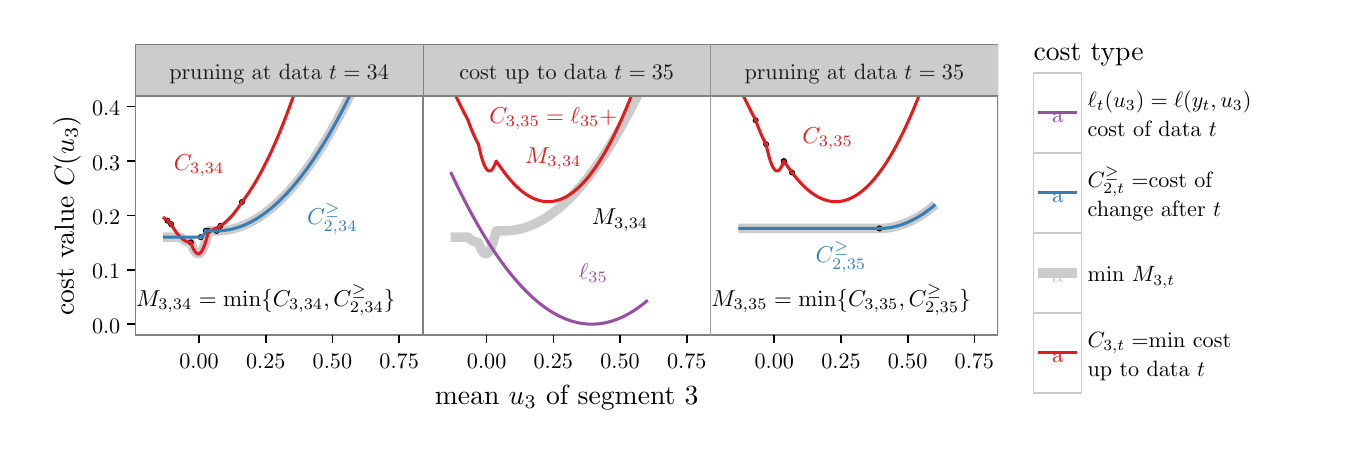
\begin{tikzpicture}[x=1pt,y=1pt]
\definecolor{fillColor}{RGB}{255,255,255}
\path[use as bounding box,fill=fillColor,fill opacity=0.00] (0,0) rectangle (469.75,144.54);
\begin{scope}
\path[clip] (  0.00,  0.00) rectangle (469.75,144.54);
\definecolor{drawColor}{RGB}{255,255,255}
\definecolor{fillColor}{RGB}{255,255,255}

\path[draw=drawColor,line width= 0.6pt,line join=round,line cap=round,fill=fillColor] (  0.00, -0.00) rectangle (469.76,144.54);
\end{scope}
\begin{scope}
\path[clip] ( 38.87,119.93) rectangle (142.81,138.54);
\definecolor{drawColor}{gray}{0.50}
\definecolor{fillColor}{gray}{0.80}

\path[draw=drawColor,line width= 0.2pt,line join=round,line cap=round,fill=fillColor] ( 38.87,119.93) rectangle (142.81,138.54);
\definecolor{drawColor}{gray}{0.10}

\node[text=drawColor,anchor=base,inner sep=0pt, outer sep=0pt, scale=  0.80] at ( 90.84,125.93) {pruning at data $t=34$};
\end{scope}
\begin{scope}
\path[clip] (142.81,119.93) rectangle (246.74,138.54);
\definecolor{drawColor}{gray}{0.50}
\definecolor{fillColor}{gray}{0.80}

\path[draw=drawColor,line width= 0.2pt,line join=round,line cap=round,fill=fillColor] (142.81,119.93) rectangle (246.74,138.54);
\definecolor{drawColor}{gray}{0.10}

\node[text=drawColor,anchor=base,inner sep=0pt, outer sep=0pt, scale=  0.80] at (194.77,125.93) {cost up to data $t=35$};
\end{scope}
\begin{scope}
\path[clip] (246.74,119.93) rectangle (350.67,138.54);
\definecolor{drawColor}{gray}{0.50}
\definecolor{fillColor}{gray}{0.80}

\path[draw=drawColor,line width= 0.2pt,line join=round,line cap=round,fill=fillColor] (246.74,119.93) rectangle (350.67,138.54);
\definecolor{drawColor}{gray}{0.10}

\node[text=drawColor,anchor=base,inner sep=0pt, outer sep=0pt, scale=  0.80] at (298.71,125.93) {pruning at data $t=35$};
\end{scope}
\begin{scope}
\path[clip] ( 38.87, 33.48) rectangle (142.81,119.93);
\definecolor{fillColor}{RGB}{255,255,255}

\path[fill=fillColor] ( 38.87, 33.48) rectangle (142.81,119.93);
\definecolor{drawColor}{gray}{0.80}

\path[draw=drawColor,line width= 3.4pt,line join=round] ( 48.91, 68.84) --
	( 48.98, 68.84) --
	( 49.04, 68.84) --
	( 49.10, 68.84) --
	( 49.17, 68.84) --
	( 49.23, 68.84) --
	( 49.29, 68.84) --
	( 49.36, 68.84) --
	( 49.42, 68.84) --
	( 49.48, 68.84) --
	( 49.55, 68.84) --
	( 49.61, 68.84) --
	( 49.67, 68.84) --
	( 49.74, 68.84) --
	( 49.80, 68.84) --
	( 49.86, 68.84) --
	( 49.93, 68.84) --
	( 49.99, 68.84) --
	( 50.06, 68.84) --
	( 50.12, 68.84) --
	( 50.18, 68.84) --
	( 50.25, 68.84) --
	( 50.31, 68.84) --
	( 50.37, 68.84) --
	( 50.44, 68.84) --
	( 50.50, 68.84) --
	( 50.56, 68.84) --
	( 50.63, 68.84) --
	( 50.69, 68.84) --
	( 50.75, 68.84) --
	( 50.82, 68.84) --
	( 50.88, 68.84) --
	( 50.94, 68.84) --
	( 51.01, 68.84) --
	( 51.07, 68.84) --
	( 51.14, 68.84) --
	( 51.20, 68.84) --
	( 51.26, 68.84) --
	( 51.33, 68.84) --
	( 51.39, 68.84) --
	( 51.45, 68.84) --
	( 51.52, 68.84) --
	( 51.58, 68.84) --
	( 51.64, 68.84) --
	( 51.71, 68.84) --
	( 51.77, 68.84) --
	( 51.83, 68.84) --
	( 51.90, 68.84) --
	( 51.96, 68.84) --
	( 52.02, 68.84) --
	( 52.09, 68.84) --
	( 52.15, 68.84) --
	( 52.22, 68.84) --
	( 52.28, 68.84) --
	( 52.34, 68.84) --
	( 52.41, 68.84) --
	( 52.47, 68.84) --
	( 52.53, 68.84) --
	( 52.60, 68.84) --
	( 52.66, 68.84) --
	( 52.72, 68.84) --
	( 52.79, 68.84) --
	( 52.85, 68.84) --
	( 52.91, 68.84) --
	( 52.98, 68.84) --
	( 53.04, 68.84) --
	( 53.10, 68.84) --
	( 53.17, 68.84) --
	( 53.23, 68.84) --
	( 53.30, 68.84) --
	( 53.36, 68.84) --
	( 53.42, 68.84) --
	( 53.49, 68.84) --
	( 53.55, 68.84) --
	( 53.61, 68.84) --
	( 53.68, 68.84) --
	( 53.74, 68.84) --
	( 53.80, 68.84) --
	( 53.87, 68.84) --
	( 53.93, 68.84) --
	( 53.99, 68.84) --
	( 54.06, 68.84) --
	( 54.12, 68.84) --
	( 54.18, 68.84) --
	( 54.25, 68.84) --
	( 54.31, 68.84) --
	( 54.38, 68.84) --
	( 54.44, 68.84) --
	( 54.50, 68.84) --
	( 54.57, 68.84) --
	( 54.63, 68.84) --
	( 54.69, 68.84) --
	( 54.76, 68.84) --
	( 54.82, 68.84) --
	( 54.88, 68.84) --
	( 54.95, 68.84) --
	( 55.01, 68.84) --
	( 55.07, 68.84) --
	( 55.14, 68.84) --
	( 55.20, 68.84) --
	( 55.20, 68.84) --
	( 55.24, 68.80) --
	( 55.28, 68.76) --
	( 55.32, 68.73) --
	( 55.35, 68.69) --
	( 55.39, 68.66) --
	( 55.43, 68.62) --
	( 55.47, 68.59) --
	( 55.51, 68.55) --
	( 55.54, 68.52) --
	( 55.58, 68.48) --
	( 55.62, 68.45) --
	( 55.66, 68.42) --
	( 55.69, 68.39) --
	( 55.73, 68.35) --
	( 55.77, 68.32) --
	( 55.81, 68.29) --
	( 55.85, 68.26) --
	( 55.88, 68.23) --
	( 55.92, 68.20) --
	( 55.96, 68.17) --
	( 56.00, 68.14) --
	( 56.04, 68.11) --
	( 56.07, 68.08) --
	( 56.11, 68.05) --
	( 56.15, 68.02) --
	( 56.19, 68.00) --
	( 56.23, 67.97) --
	( 56.26, 67.94) --
	( 56.30, 67.92) --
	( 56.34, 67.89) --
	( 56.38, 67.86) --
	( 56.42, 67.84) --
	( 56.45, 67.81) --
	( 56.49, 67.79) --
	( 56.53, 67.76) --
	( 56.57, 67.74) --
	( 56.61, 67.72) --
	( 56.64, 67.69) --
	( 56.68, 67.67) --
	( 56.72, 67.65) --
	( 56.76, 67.62) --
	( 56.80, 67.60) --
	( 56.83, 67.58) --
	( 56.87, 67.56) --
	( 56.91, 67.54) --
	( 56.95, 67.52) --
	( 56.99, 67.50) --
	( 57.02, 67.48) --
	( 57.06, 67.46) --
	( 57.10, 67.44) --
	( 57.14, 67.42) --
	( 57.17, 67.40) --
	( 57.21, 67.39) --
	( 57.25, 67.37) --
	( 57.29, 67.35) --
	( 57.33, 67.33) --
	( 57.36, 67.32) --
	( 57.40, 67.30) --
	( 57.44, 67.29) --
	( 57.48, 67.27) --
	( 57.52, 67.26) --
	( 57.55, 67.24) --
	( 57.59, 67.23) --
	( 57.63, 67.21) --
	( 57.67, 67.20) --
	( 57.71, 67.19) --
	( 57.74, 67.17) --
	( 57.78, 67.16) --
	( 57.82, 67.15) --
	( 57.86, 67.14) --
	( 57.90, 67.13) --
	( 57.93, 67.11) --
	( 57.97, 67.10) --
	( 58.01, 67.09) --
	( 58.05, 67.08) --
	( 58.09, 67.07) --
	( 58.12, 67.07) --
	( 58.16, 67.06) --
	( 58.20, 67.05) --
	( 58.24, 67.04) --
	( 58.28, 67.03) --
	( 58.31, 67.03) --
	( 58.35, 67.02) --
	( 58.39, 67.01) --
	( 58.43, 67.01) --
	( 58.47, 67.00) --
	( 58.50, 66.99) --
	( 58.54, 66.99) --
	( 58.58, 66.98) --
	( 58.62, 66.98) --
	( 58.65, 66.98) --
	( 58.69, 66.97) --
	( 58.73, 66.97) --
	( 58.77, 66.97) --
	( 58.81, 66.96) --
	( 58.84, 66.96) --
	( 58.88, 66.96) --
	( 58.92, 66.96) --
	( 58.96, 66.96) --
	( 58.96, 66.96) --
	( 59.02, 66.76) --
	( 59.09, 66.56) --
	( 59.15, 66.38) --
	( 59.22, 66.19) --
	( 59.28, 66.01) --
	( 59.34, 65.84) --
	( 59.41, 65.67) --
	( 59.47, 65.50) --
	( 59.54, 65.34) --
	( 59.60, 65.19) --
	( 59.67, 65.04) --
	( 59.73, 64.89) --
	( 59.80, 64.75) --
	( 59.86, 64.62) --
	( 59.92, 64.49) --
	( 59.99, 64.36) --
	( 60.05, 64.24) --
	( 60.12, 64.13) --
	( 60.18, 64.02) --
	( 60.25, 63.91) --
	( 60.31, 63.81) --
	( 60.38, 63.72) --
	( 60.44, 63.62) --
	( 60.50, 63.54) --
	( 60.57, 63.46) --
	( 60.63, 63.38) --
	( 60.70, 63.31) --
	( 60.76, 63.24) --
	( 60.83, 63.18) --
	( 60.89, 63.12) --
	( 60.95, 63.07) --
	( 61.02, 63.03) --
	( 61.08, 62.98) --
	( 61.15, 62.95) --
	( 61.21, 62.92) --
	( 61.28, 62.89) --
	( 61.34, 62.87) --
	( 61.41, 62.85) --
	( 61.47, 62.84) --
	( 61.53, 62.83) --
	( 61.60, 62.83) --
	( 61.66, 62.83) --
	( 61.73, 62.84) --
	( 61.79, 62.85) --
	( 61.86, 62.86) --
	( 61.92, 62.89) --
	( 61.98, 62.91) --
	( 62.05, 62.95) --
	( 62.11, 62.98) --
	( 62.18, 63.02) --
	( 62.24, 63.07) --
	( 62.31, 63.12) --
	( 62.37, 63.18) --
	( 62.44, 63.24) --
	( 62.50, 63.30) --
	( 62.56, 63.38) --
	( 62.63, 63.45) --
	( 62.69, 63.53) --
	( 62.76, 63.62) --
	( 62.82, 63.71) --
	( 62.89, 63.80) --
	( 62.95, 63.90) --
	( 63.01, 64.01) --
	( 63.08, 64.12) --
	( 63.14, 64.24) --
	( 63.21, 64.36) --
	( 63.27, 64.48) --
	( 63.34, 64.61) --
	( 63.40, 64.75) --
	( 63.47, 64.88) --
	( 63.53, 65.03) --
	( 63.59, 65.18) --
	( 63.66, 65.33) --
	( 63.72, 65.49) --
	( 63.79, 65.66) --
	( 63.85, 65.83) --
	( 63.92, 66.00) --
	( 63.98, 66.18) --
	( 64.05, 66.36) --
	( 64.11, 66.55) --
	( 64.17, 66.75) --
	( 64.24, 66.94) --
	( 64.30, 67.15) --
	( 64.37, 67.36) --
	( 64.43, 67.57) --
	( 64.50, 67.79) --
	( 64.56, 68.01) --
	( 64.62, 68.24) --
	( 64.69, 68.47) --
	( 64.75, 68.71) --
	( 64.82, 68.95) --
	( 64.88, 69.20) --
	( 64.95, 69.45) --
	( 65.01, 69.71) --
	( 65.08, 69.97) --
	( 65.14, 70.24) --
	( 65.20, 70.51) --
	( 65.27, 70.79) --
	( 65.33, 71.07) --
	( 65.33, 71.07) --
	( 65.33, 71.07) --
	( 65.34, 71.07) --
	( 65.34, 71.07) --
	( 65.34, 71.07) --
	( 65.34, 71.07) --
	( 65.35, 71.07) --
	( 65.35, 71.07) --
	( 65.35, 71.07) --
	( 65.35, 71.08) --
	( 65.35, 71.08) --
	( 65.36, 71.08) --
	( 65.36, 71.08) --
	( 65.36, 71.08) --
	( 65.36, 71.08) --
	( 65.36, 71.08) --
	( 65.37, 71.08) --
	( 65.37, 71.08) --
	( 65.37, 71.08) --
	( 65.37, 71.08) --
	( 65.37, 71.08) --
	( 65.38, 71.08) --
	( 65.38, 71.08) --
	( 65.38, 71.08) --
	( 65.38, 71.08) --
	( 65.38, 71.08) --
	( 65.39, 71.08) --
	( 65.39, 71.08) --
	( 65.39, 71.08) --
	( 65.39, 71.09) --
	( 65.39, 71.09) --
	( 65.40, 71.09) --
	( 65.40, 71.09) --
	( 65.40, 71.09) --
	( 65.40, 71.09) --
	( 65.40, 71.09) --
	( 65.41, 71.09) --
	( 65.41, 71.09) --
	( 65.41, 71.09) --
	( 65.41, 71.09) --
	( 65.41, 71.09) --
	( 65.42, 71.09) --
	( 65.42, 71.09) --
	( 65.42, 71.09) --
	( 65.42, 71.09) --
	( 65.42, 71.09) --
	( 65.43, 71.09) --
	( 65.43, 71.09) --
	( 65.43, 71.10) --
	( 65.43, 71.10) --
	( 65.43, 71.10) --
	( 65.44, 71.10) --
	( 65.44, 71.10) --
	( 65.44, 71.10) --
	( 65.44, 71.10) --
	( 65.44, 71.10) --
	( 65.45, 71.10) --
	( 65.45, 71.10) --
	( 65.45, 71.10) --
	( 65.45, 71.10) --
	( 65.46, 71.10) --
	( 65.46, 71.10) --
	( 65.46, 71.10) --
	( 65.46, 71.10) --
	( 65.46, 71.10) --
	( 65.47, 71.10) --
	( 65.47, 71.10) --
	( 65.47, 71.11) --
	( 65.47, 71.11) --
	( 65.47, 71.11) --
	( 65.48, 71.11) --
	( 65.48, 71.11) --
	( 65.48, 71.11) --
	( 65.48, 71.11) --
	( 65.48, 71.11) --
	( 65.49, 71.11) --
	( 65.49, 71.11) --
	( 65.49, 71.11) --
	( 65.49, 71.11) --
	( 65.49, 71.11) --
	( 65.50, 71.11) --
	( 65.50, 71.11) --
	( 65.50, 71.11) --
	( 65.50, 71.11) --
	( 65.50, 71.11) --
	( 65.51, 71.11) --
	( 65.51, 71.12) --
	( 65.51, 71.12) --
	( 65.51, 71.12) --
	( 65.51, 71.12) --
	( 65.52, 71.12) --
	( 65.52, 71.12) --
	( 65.52, 71.12) --
	( 65.52, 71.12) --
	( 65.52, 71.12) --
	( 65.53, 71.12) --
	( 65.53, 71.12) --
	( 65.53, 71.12) --
	( 65.53, 71.12) --
	( 65.53, 71.12) --
	( 65.53, 71.12) --
	( 65.56, 71.12) --
	( 65.59, 71.12) --
	( 65.62, 71.12) --
	( 65.65, 71.12) --
	( 65.68, 71.12) --
	( 65.70, 71.12) --
	( 65.73, 71.12) --
	( 65.76, 71.12) --
	( 65.79, 71.12) --
	( 65.82, 71.12) --
	( 65.84, 71.12) --
	( 65.87, 71.12) --
	( 65.90, 71.12) --
	( 65.93, 71.12) --
	( 65.96, 71.12) --
	( 65.98, 71.12) --
	( 66.01, 71.12) --
	( 66.04, 71.12) --
	( 66.07, 71.12) --
	( 66.10, 71.12) --
	( 66.13, 71.12) --
	( 66.15, 71.12) --
	( 66.18, 71.12) --
	( 66.21, 71.12) --
	( 66.24, 71.12) --
	( 66.27, 71.12) --
	( 66.29, 71.12) --
	( 66.32, 71.12) --
	( 66.35, 71.12) --
	( 66.38, 71.12) --
	( 66.41, 71.12) --
	( 66.43, 71.12) --
	( 66.46, 71.12) --
	( 66.49, 71.12) --
	( 66.52, 71.12) --
	( 66.55, 71.12) --
	( 66.58, 71.12) --
	( 66.60, 71.12) --
	( 66.63, 71.12) --
	( 66.66, 71.12) --
	( 66.69, 71.12) --
	( 66.72, 71.12) --
	( 66.74, 71.12) --
	( 66.77, 71.12) --
	( 66.80, 71.12) --
	( 66.83, 71.12) --
	( 66.86, 71.12) --
	( 66.89, 71.12) --
	( 66.91, 71.12) --
	( 66.94, 71.12) --
	( 66.97, 71.12) --
	( 67.00, 71.12) --
	( 67.03, 71.12) --
	( 67.05, 71.12) --
	( 67.08, 71.12) --
	( 67.11, 71.12) --
	( 67.14, 71.12) --
	( 67.17, 71.12) --
	( 67.19, 71.12) --
	( 67.22, 71.12) --
	( 67.25, 71.12) --
	( 67.28, 71.12) --
	( 67.31, 71.12) --
	( 67.34, 71.12) --
	( 67.36, 71.12) --
	( 67.39, 71.12) --
	( 67.42, 71.12) --
	( 67.45, 71.12) --
	( 67.48, 71.12) --
	( 67.50, 71.12) --
	( 67.53, 71.12) --
	( 67.56, 71.12) --
	( 67.59, 71.12) --
	( 67.62, 71.12) --
	( 67.64, 71.12) --
	( 67.67, 71.12) --
	( 67.70, 71.12) --
	( 67.73, 71.12) --
	( 67.76, 71.12) --
	( 67.79, 71.12) --
	( 67.81, 71.12) --
	( 67.84, 71.12) --
	( 67.87, 71.12) --
	( 67.90, 71.12) --
	( 67.93, 71.12) --
	( 67.95, 71.12) --
	( 67.98, 71.12) --
	( 68.01, 71.12) --
	( 68.04, 71.12) --
	( 68.07, 71.12) --
	( 68.10, 71.12) --
	( 68.12, 71.12) --
	( 68.15, 71.12) --
	( 68.18, 71.12) --
	( 68.21, 71.12) --
	( 68.24, 71.12) --
	( 68.26, 71.12) --
	( 68.29, 71.12) --
	( 68.32, 71.12) --
	( 68.32, 71.12) --
	( 68.84, 71.13) --
	( 69.37, 71.15) --
	( 69.89, 71.17) --
	( 70.41, 71.22) --
	( 70.94, 71.27) --
	( 71.46, 71.33) --
	( 71.98, 71.41) --
	( 72.51, 71.49) --
	( 73.03, 71.59) --
	( 73.55, 71.70) --
	( 74.08, 71.82) --
	( 74.60, 71.96) --
	( 75.12, 72.10) --
	( 75.65, 72.26) --
	( 76.17, 72.43) --
	( 76.69, 72.60) --
	( 77.22, 72.80) --
	( 77.74, 73.00) --
	( 78.26, 73.21) --
	( 78.79, 73.44) --
	( 79.31, 73.68) --
	( 79.83, 73.92) --
	( 80.36, 74.19) --
	( 80.88, 74.46) --
	( 81.40, 74.74) --
	( 81.93, 75.04) --
	( 82.45, 75.34) --
	( 82.97, 75.66) --
	( 83.50, 75.99) --
	( 84.02, 76.33) --
	( 84.54, 76.69) --
	( 85.07, 77.05) --
	( 85.59, 77.43) --
	( 86.11, 77.82) --
	( 86.64, 78.22) --
	( 87.16, 78.63) --
	( 87.68, 79.05) --
	( 88.21, 79.48) --
	( 88.73, 79.93) --
	( 89.26, 80.39) --
	( 89.78, 80.86) --
	( 90.30, 81.34) --
	( 90.83, 81.83) --
	( 91.35, 82.33) --
	( 91.87, 82.85) --
	( 92.40, 83.37) --
	( 92.92, 83.91) --
	( 93.44, 84.46) --
	( 93.97, 85.02) --
	( 94.49, 85.60) --
	( 95.01, 86.18) --
	( 95.54, 86.78) --
	( 96.06, 87.39) --
	( 96.58, 88.01) --
	( 97.11, 88.64) --
	( 97.63, 89.28) --
	( 98.15, 89.93) --
	( 98.68, 90.60) --
	( 99.20, 91.28) --
	( 99.72, 91.97) --
	(100.25, 92.67) --
	(100.77, 93.38) --
	(101.29, 94.10) --
	(101.82, 94.84) --
	(102.34, 95.58) --
	(102.86, 96.34) --
	(103.39, 97.11) --
	(103.91, 97.89) --
	(104.43, 98.69) --
	(104.96, 99.49) --
	(105.48,100.31) --
	(106.00,101.14) --
	(106.53,101.98) --
	(107.05,102.83) --
	(107.57,103.69) --
	(108.10,104.56) --
	(108.62,105.45) --
	(109.14,106.35) --
	(109.67,107.26) --
	(110.19,108.18) --
	(110.71,109.11) --
	(111.24,110.05) --
	(111.76,111.01) --
	(112.28,111.98) --
	(112.81,112.95) --
	(113.33,113.94) --
	(113.85,114.95) --
	(114.38,115.96) --
	(114.90,116.98) --
	(115.42,118.02) --
	(115.95,119.07) --
	(116.47,120.13) --
	(116.99,121.20) --
	(117.52,122.28) --
	(118.04,123.38) --
	(118.56,124.48) --
	(119.09,125.60) --
	(119.61,126.73) --
	(120.13,127.87);
\definecolor{drawColor}{RGB}{0,0,0}

\path[draw=drawColor,line width= 0.4pt,line join=round,line cap=round] ( 62.52, 68.84) circle (  0.89);

\path[draw=drawColor,line width= 0.4pt,line join=round,line cap=round] ( 64.36, 71.12) circle (  0.89);

\path[draw=drawColor,line width= 0.4pt,line join=round,line cap=round] ( 68.32, 71.12) circle (  0.89);

\path[draw=drawColor,line width= 0.4pt,line join=round,line cap=round] ( 50.49, 74.82) circle (  0.89);

\path[draw=drawColor,line width= 0.4pt,line join=round,line cap=round] ( 51.85, 73.53) circle (  0.89);

\path[draw=drawColor,line width= 0.4pt,line join=round,line cap=round] ( 58.96, 66.96) circle (  0.89);

\path[draw=drawColor,line width= 0.4pt,line join=round,line cap=round] ( 65.33, 71.07) circle (  0.89);

\path[draw=drawColor,line width= 0.4pt,line join=round,line cap=round] ( 69.64, 72.92) circle (  0.89);

\path[draw=drawColor,line width= 0.4pt,line join=round,line cap=round] ( 77.42, 81.54) circle (  0.89);
\definecolor{drawColor}{RGB}{228,26,28}

\path[draw=drawColor,line width= 1.1pt,line join=round] ( 48.91, 76.07) --
	( 48.93, 76.05) --
	( 48.94, 76.04) --
	( 48.96, 76.03) --
	( 48.98, 76.01) --
	( 48.99, 76.00) --
	( 49.01, 75.99) --
	( 49.02, 75.97) --
	( 49.04, 75.96) --
	( 49.05, 75.95) --
	( 49.07, 75.94) --
	( 49.09, 75.92) --
	( 49.10, 75.91) --
	( 49.12, 75.90) --
	( 49.13, 75.88) --
	( 49.15, 75.87) --
	( 49.17, 75.86) --
	( 49.18, 75.84) --
	( 49.20, 75.83) --
	( 49.21, 75.82) --
	( 49.23, 75.81) --
	( 49.25, 75.79) --
	( 49.26, 75.78) --
	( 49.28, 75.77) --
	( 49.29, 75.75) --
	( 49.31, 75.74) --
	( 49.33, 75.73) --
	( 49.34, 75.72) --
	( 49.36, 75.70) --
	( 49.37, 75.69) --
	( 49.39, 75.68) --
	( 49.41, 75.67) --
	( 49.42, 75.65) --
	( 49.44, 75.64) --
	( 49.45, 75.63) --
	( 49.47, 75.61) --
	( 49.48, 75.60) --
	( 49.50, 75.59) --
	( 49.52, 75.58) --
	( 49.53, 75.56) --
	( 49.55, 75.55) --
	( 49.56, 75.54) --
	( 49.58, 75.53) --
	( 49.60, 75.51) --
	( 49.61, 75.50) --
	( 49.63, 75.49) --
	( 49.64, 75.48) --
	( 49.66, 75.46) --
	( 49.68, 75.45) --
	( 49.69, 75.44) --
	( 49.71, 75.43) --
	( 49.72, 75.41) --
	( 49.74, 75.40) --
	( 49.76, 75.39) --
	( 49.77, 75.38) --
	( 49.79, 75.36) --
	( 49.80, 75.35) --
	( 49.82, 75.34) --
	( 49.84, 75.33) --
	( 49.85, 75.31) --
	( 49.87, 75.30) --
	( 49.88, 75.29) --
	( 49.90, 75.28) --
	( 49.92, 75.26) --
	( 49.93, 75.25) --
	( 49.95, 75.24) --
	( 49.96, 75.23) --
	( 49.98, 75.21) --
	( 49.99, 75.20) --
	( 50.01, 75.19) --
	( 50.03, 75.18) --
	( 50.04, 75.16) --
	( 50.06, 75.15) --
	( 50.07, 75.14) --
	( 50.09, 75.13) --
	( 50.11, 75.12) --
	( 50.12, 75.10) --
	( 50.14, 75.09) --
	( 50.15, 75.08) --
	( 50.17, 75.07) --
	( 50.19, 75.05) --
	( 50.20, 75.04) --
	( 50.22, 75.03) --
	( 50.23, 75.02) --
	( 50.25, 75.01) --
	( 50.27, 74.99) --
	( 50.28, 74.98) --
	( 50.30, 74.97) --
	( 50.31, 74.96) --
	( 50.33, 74.94) --
	( 50.35, 74.93) --
	( 50.36, 74.92) --
	( 50.38, 74.91) --
	( 50.39, 74.90) --
	( 50.41, 74.88) --
	( 50.42, 74.87) --
	( 50.44, 74.86) --
	( 50.46, 74.85) --
	( 50.47, 74.84) --
	( 50.49, 74.82) --
	( 50.49, 74.82) --
	( 50.50, 74.81) --
	( 50.52, 74.80) --
	( 50.53, 74.78) --
	( 50.54, 74.77) --
	( 50.56, 74.75) --
	( 50.57, 74.74) --
	( 50.58, 74.73) --
	( 50.60, 74.71) --
	( 50.61, 74.70) --
	( 50.63, 74.69) --
	( 50.64, 74.67) --
	( 50.65, 74.66) --
	( 50.67, 74.65) --
	( 50.68, 74.63) --
	( 50.69, 74.62) --
	( 50.71, 74.60) --
	( 50.72, 74.59) --
	( 50.74, 74.58) --
	( 50.75, 74.56) --
	( 50.76, 74.55) --
	( 50.78, 74.54) --
	( 50.79, 74.52) --
	( 50.81, 74.51) --
	( 50.82, 74.50) --
	( 50.83, 74.48) --
	( 50.85, 74.47) --
	( 50.86, 74.46) --
	( 50.87, 74.44) --
	( 50.89, 74.43) --
	( 50.90, 74.42) --
	( 50.92, 74.40) --
	( 50.93, 74.39) --
	( 50.94, 74.38) --
	( 50.96, 74.36) --
	( 50.97, 74.35) --
	( 50.98, 74.34) --
	( 51.00, 74.32) --
	( 51.01, 74.31) --
	( 51.03, 74.30) --
	( 51.04, 74.28) --
	( 51.05, 74.27) --
	( 51.07, 74.26) --
	( 51.08, 74.24) --
	( 51.09, 74.23) --
	( 51.11, 74.22) --
	( 51.12, 74.20) --
	( 51.14, 74.19) --
	( 51.15, 74.18) --
	( 51.16, 74.16) --
	( 51.18, 74.15) --
	( 51.19, 74.14) --
	( 51.20, 74.13) --
	( 51.22, 74.11) --
	( 51.23, 74.10) --
	( 51.25, 74.09) --
	( 51.26, 74.07) --
	( 51.27, 74.06) --
	( 51.29, 74.05) --
	( 51.30, 74.03) --
	( 51.31, 74.02) --
	( 51.33, 74.01) --
	( 51.34, 74.00) --
	( 51.36, 73.98) --
	( 51.37, 73.97) --
	( 51.38, 73.96) --
	( 51.40, 73.94) --
	( 51.41, 73.93) --
	( 51.42, 73.92) --
	( 51.44, 73.91) --
	( 51.45, 73.89) --
	( 51.47, 73.88) --
	( 51.48, 73.87) --
	( 51.49, 73.86) --
	( 51.51, 73.84) --
	( 51.52, 73.83) --
	( 51.54, 73.82) --
	( 51.55, 73.80) --
	( 51.56, 73.79) --
	( 51.58, 73.78) --
	( 51.59, 73.77) --
	( 51.60, 73.75) --
	( 51.62, 73.74) --
	( 51.63, 73.73) --
	( 51.65, 73.72) --
	( 51.66, 73.70) --
	( 51.67, 73.69) --
	( 51.69, 73.68) --
	( 51.70, 73.67) --
	( 51.71, 73.65) --
	( 51.73, 73.64) --
	( 51.74, 73.63) --
	( 51.76, 73.62) --
	( 51.77, 73.60) --
	( 51.78, 73.59) --
	( 51.80, 73.58) --
	( 51.81, 73.57) --
	( 51.82, 73.56) --
	( 51.84, 73.54) --
	( 51.85, 73.53) --
	( 51.85, 73.53) --
	( 51.92, 73.40) --
	( 52.00, 73.27) --
	( 52.07, 73.14) --
	( 52.14, 73.02) --
	( 52.21, 72.89) --
	( 52.28, 72.77) --
	( 52.35, 72.64) --
	( 52.43, 72.52) --
	( 52.50, 72.40) --
	( 52.57, 72.29) --
	( 52.64, 72.17) --
	( 52.71, 72.05) --
	( 52.78, 71.94) --
	( 52.86, 71.82) --
	( 52.93, 71.71) --
	( 53.00, 71.60) --
	( 53.07, 71.49) --
	( 53.14, 71.38) --
	( 53.22, 71.28) --
	( 53.29, 71.17) --
	( 53.36, 71.07) --
	( 53.43, 70.96) --
	( 53.50, 70.86) --
	( 53.57, 70.76) --
	( 53.65, 70.66) --
	( 53.72, 70.56) --
	( 53.79, 70.47) --
	( 53.86, 70.37) --
	( 53.93, 70.28) --
	( 54.01, 70.19) --
	( 54.08, 70.09) --
	( 54.15, 70.00) --
	( 54.22, 69.92) --
	( 54.29, 69.83) --
	( 54.36, 69.74) --
	( 54.44, 69.66) --
	( 54.51, 69.57) --
	( 54.58, 69.49) --
	( 54.65, 69.41) --
	( 54.72, 69.33) --
	( 54.79, 69.25) --
	( 54.87, 69.18) --
	( 54.94, 69.10) --
	( 55.01, 69.03) --
	( 55.08, 68.95) --
	( 55.15, 68.88) --
	( 55.23, 68.81) --
	( 55.30, 68.74) --
	( 55.37, 68.68) --
	( 55.44, 68.61) --
	( 55.51, 68.54) --
	( 55.58, 68.48) --
	( 55.66, 68.42) --
	( 55.73, 68.36) --
	( 55.80, 68.30) --
	( 55.87, 68.24) --
	( 55.94, 68.18) --
	( 56.02, 68.13) --
	( 56.09, 68.07) --
	( 56.16, 68.02) --
	( 56.23, 67.97) --
	( 56.30, 67.91) --
	( 56.37, 67.87) --
	( 56.45, 67.82) --
	( 56.52, 67.77) --
	( 56.59, 67.73) --
	( 56.66, 67.68) --
	( 56.73, 67.64) --
	( 56.80, 67.60) --
	( 56.88, 67.56) --
	( 56.95, 67.52) --
	( 57.02, 67.48) --
	( 57.09, 67.44) --
	( 57.16, 67.41) --
	( 57.24, 67.37) --
	( 57.31, 67.34) --
	( 57.38, 67.31) --
	( 57.45, 67.28) --
	( 57.52, 67.25) --
	( 57.59, 67.23) --
	( 57.67, 67.20) --
	( 57.74, 67.18) --
	( 57.81, 67.15) --
	( 57.88, 67.13) --
	( 57.95, 67.11) --
	( 58.03, 67.09) --
	( 58.10, 67.07) --
	( 58.17, 67.06) --
	( 58.24, 67.04) --
	( 58.31, 67.03) --
	( 58.38, 67.01) --
	( 58.46, 67.00) --
	( 58.53, 66.99) --
	( 58.60, 66.98) --
	( 58.67, 66.97) --
	( 58.74, 66.97) --
	( 58.81, 66.96) --
	( 58.89, 66.96) --
	( 58.96, 66.96) --
	( 58.96, 66.96) --
	( 59.02, 66.76) --
	( 59.09, 66.56) --
	( 59.15, 66.38) --
	( 59.22, 66.19) --
	( 59.28, 66.01) --
	( 59.34, 65.84) --
	( 59.41, 65.67) --
	( 59.47, 65.50) --
	( 59.54, 65.34) --
	( 59.60, 65.19) --
	( 59.67, 65.04) --
	( 59.73, 64.89) --
	( 59.80, 64.75) --
	( 59.86, 64.62) --
	( 59.92, 64.49) --
	( 59.99, 64.36) --
	( 60.05, 64.24) --
	( 60.12, 64.13) --
	( 60.18, 64.02) --
	( 60.25, 63.91) --
	( 60.31, 63.81) --
	( 60.38, 63.72) --
	( 60.44, 63.62) --
	( 60.50, 63.54) --
	( 60.57, 63.46) --
	( 60.63, 63.38) --
	( 60.70, 63.31) --
	( 60.76, 63.24) --
	( 60.83, 63.18) --
	( 60.89, 63.12) --
	( 60.95, 63.07) --
	( 61.02, 63.03) --
	( 61.08, 62.98) --
	( 61.15, 62.95) --
	( 61.21, 62.92) --
	( 61.28, 62.89) --
	( 61.34, 62.87) --
	( 61.41, 62.85) --
	( 61.47, 62.84) --
	( 61.53, 62.83) --
	( 61.60, 62.83) --
	( 61.66, 62.83) --
	( 61.73, 62.84) --
	( 61.79, 62.85) --
	( 61.86, 62.86) --
	( 61.92, 62.89) --
	( 61.98, 62.91) --
	( 62.05, 62.95) --
	( 62.11, 62.98) --
	( 62.18, 63.02) --
	( 62.24, 63.07) --
	( 62.31, 63.12) --
	( 62.37, 63.18) --
	( 62.44, 63.24) --
	( 62.50, 63.30) --
	( 62.56, 63.38) --
	( 62.63, 63.45) --
	( 62.69, 63.53) --
	( 62.76, 63.62) --
	( 62.82, 63.71) --
	( 62.89, 63.80) --
	( 62.95, 63.90) --
	( 63.01, 64.01) --
	( 63.08, 64.12) --
	( 63.14, 64.24) --
	( 63.21, 64.36) --
	( 63.27, 64.48) --
	( 63.34, 64.61) --
	( 63.40, 64.75) --
	( 63.47, 64.88) --
	( 63.53, 65.03) --
	( 63.59, 65.18) --
	( 63.66, 65.33) --
	( 63.72, 65.49) --
	( 63.79, 65.66) --
	( 63.85, 65.83) --
	( 63.92, 66.00) --
	( 63.98, 66.18) --
	( 64.05, 66.36) --
	( 64.11, 66.55) --
	( 64.17, 66.75) --
	( 64.24, 66.94) --
	( 64.30, 67.15) --
	( 64.37, 67.36) --
	( 64.43, 67.57) --
	( 64.50, 67.79) --
	( 64.56, 68.01) --
	( 64.62, 68.24) --
	( 64.69, 68.47) --
	( 64.75, 68.71) --
	( 64.82, 68.95) --
	( 64.88, 69.20) --
	( 64.95, 69.45) --
	( 65.01, 69.71) --
	( 65.08, 69.97) --
	( 65.14, 70.24) --
	( 65.20, 70.51) --
	( 65.27, 70.79) --
	( 65.33, 71.07) --
	( 65.33, 71.07) --
	( 65.38, 71.08) --
	( 65.42, 71.09) --
	( 65.46, 71.10) --
	( 65.51, 71.12) --
	( 65.55, 71.13) --
	( 65.59, 71.14) --
	( 65.64, 71.15) --
	( 65.68, 71.16) --
	( 65.72, 71.17) --
	( 65.77, 71.19) --
	( 65.81, 71.20) --
	( 65.85, 71.21) --
	( 65.90, 71.22) --
	( 65.94, 71.24) --
	( 65.99, 71.25) --
	( 66.03, 71.26) --
	( 66.07, 71.28) --
	( 66.12, 71.29) --
	( 66.16, 71.30) --
	( 66.20, 71.32) --
	( 66.25, 71.33) --
	( 66.29, 71.35) --
	( 66.33, 71.36) --
	( 66.38, 71.38) --
	( 66.42, 71.39) --
	( 66.46, 71.41) --
	( 66.51, 71.42) --
	( 66.55, 71.44) --
	( 66.59, 71.45) --
	( 66.64, 71.47) --
	( 66.68, 71.48) --
	( 66.72, 71.50) --
	( 66.77, 71.51) --
	( 66.81, 71.53) --
	( 66.85, 71.55) --
	( 66.90, 71.56) --
	( 66.94, 71.58) --
	( 66.99, 71.60) --
	( 67.03, 71.61) --
	( 67.07, 71.63) --
	( 67.12, 71.65) --
	( 67.16, 71.67) --
	( 67.20, 71.68) --
	( 67.25, 71.70) --
	( 67.29, 71.72) --
	( 67.33, 71.74) --
	( 67.38, 71.76) --
	( 67.42, 71.77) --
	( 67.46, 71.79) --
	( 67.51, 71.81) --
	( 67.55, 71.83) --
	( 67.59, 71.85) --
	( 67.64, 71.87) --
	( 67.68, 71.89) --
	( 67.72, 71.91) --
	( 67.77, 71.93) --
	( 67.81, 71.95) --
	( 67.85, 71.97) --
	( 67.90, 71.99) --
	( 67.94, 72.01) --
	( 67.99, 72.03) --
	( 68.03, 72.05) --
	( 68.07, 72.07) --
	( 68.12, 72.09) --
	( 68.16, 72.11) --
	( 68.20, 72.13) --
	( 68.25, 72.15) --
	( 68.29, 72.18) --
	( 68.33, 72.20) --
	( 68.38, 72.22) --
	( 68.42, 72.24) --
	( 68.46, 72.26) --
	( 68.51, 72.29) --
	( 68.55, 72.31) --
	( 68.59, 72.33) --
	( 68.64, 72.35) --
	( 68.68, 72.38) --
	( 68.72, 72.40) --
	( 68.77, 72.42) --
	( 68.81, 72.45) --
	( 68.85, 72.47) --
	( 68.90, 72.49) --
	( 68.94, 72.52) --
	( 68.99, 72.54) --
	( 69.03, 72.57) --
	( 69.07, 72.59) --
	( 69.12, 72.62) --
	( 69.16, 72.64) --
	( 69.20, 72.67) --
	( 69.25, 72.69) --
	( 69.29, 72.72) --
	( 69.33, 72.74) --
	( 69.38, 72.77) --
	( 69.42, 72.79) --
	( 69.46, 72.82) --
	( 69.51, 72.85) --
	( 69.55, 72.87) --
	( 69.59, 72.90) --
	( 69.64, 72.92) --
	( 69.64, 72.92) --
	( 69.72, 72.97) --
	( 69.79, 73.02) --
	( 69.87, 73.07) --
	( 69.95, 73.12) --
	( 70.03, 73.18) --
	( 70.11, 73.23) --
	( 70.19, 73.28) --
	( 70.27, 73.34) --
	( 70.35, 73.39) --
	( 70.42, 73.45) --
	( 70.50, 73.50) --
	( 70.58, 73.56) --
	( 70.66, 73.62) --
	( 70.74, 73.68) --
	( 70.82, 73.74) --
	( 70.90, 73.80) --
	( 70.97, 73.86) --
	( 71.05, 73.92) --
	( 71.13, 73.98) --
	( 71.21, 74.05) --
	( 71.29, 74.11) --
	( 71.37, 74.17) --
	( 71.45, 74.24) --
	( 71.52, 74.31) --
	( 71.60, 74.37) --
	( 71.68, 74.44) --
	( 71.76, 74.51) --
	( 71.84, 74.58) --
	( 71.92, 74.65) --
	( 72.00, 74.72) --
	( 72.08, 74.80) --
	( 72.15, 74.87) --
	( 72.23, 74.94) --
	( 72.31, 75.02) --
	( 72.39, 75.09) --
	( 72.47, 75.17) --
	( 72.55, 75.24) --
	( 72.63, 75.32) --
	( 72.70, 75.40) --
	( 72.78, 75.48) --
	( 72.86, 75.56) --
	( 72.94, 75.64) --
	( 73.02, 75.72) --
	( 73.10, 75.80) --
	( 73.18, 75.89) --
	( 73.26, 75.97) --
	( 73.33, 76.06) --
	( 73.41, 76.14) --
	( 73.49, 76.23) --
	( 73.57, 76.31) --
	( 73.65, 76.40) --
	( 73.73, 76.49) --
	( 73.81, 76.58) --
	( 73.88, 76.67) --
	( 73.96, 76.76) --
	( 74.04, 76.85) --
	( 74.12, 76.95) --
	( 74.20, 77.04) --
	( 74.28, 77.13) --
	( 74.36, 77.23) --
	( 74.43, 77.32) --
	( 74.51, 77.42) --
	( 74.59, 77.52) --
	( 74.67, 77.62) --
	( 74.75, 77.71) --
	( 74.83, 77.81) --
	( 74.91, 77.91) --
	( 74.99, 78.02) --
	( 75.06, 78.12) --
	( 75.14, 78.22) --
	( 75.22, 78.32) --
	( 75.30, 78.43) --
	( 75.38, 78.53) --
	( 75.46, 78.64) --
	( 75.54, 78.75) --
	( 75.61, 78.85) --
	( 75.69, 78.96) --
	( 75.77, 79.07) --
	( 75.85, 79.18) --
	( 75.93, 79.29) --
	( 76.01, 79.40) --
	( 76.09, 79.51) --
	( 76.17, 79.63) --
	( 76.24, 79.74) --
	( 76.32, 79.85) --
	( 76.40, 79.97) --
	( 76.48, 80.09) --
	( 76.56, 80.20) --
	( 76.64, 80.32) --
	( 76.72, 80.44) --
	( 76.79, 80.56) --
	( 76.87, 80.68) --
	( 76.95, 80.80) --
	( 77.03, 80.92) --
	( 77.11, 81.04) --
	( 77.19, 81.17) --
	( 77.27, 81.29) --
	( 77.34, 81.41) --
	( 77.42, 81.54) --
	( 77.42, 81.54) --
	( 77.85, 82.10) --
	( 78.29, 82.67) --
	( 78.72, 83.26) --
	( 79.15, 83.86) --
	( 79.58, 84.48) --
	( 80.01, 85.11) --
	( 80.44, 85.76) --
	( 80.87, 86.43) --
	( 81.31, 87.11) --
	( 81.74, 87.81) --
	( 82.17, 88.52) --
	( 82.60, 89.25) --
	( 83.03, 90.00) --
	( 83.46, 90.76) --
	( 83.89, 91.54) --
	( 84.33, 92.33) --
	( 84.76, 93.14) --
	( 85.19, 93.96) --
	( 85.62, 94.80) --
	( 86.05, 95.65) --
	( 86.48, 96.53) --
	( 86.91, 97.41) --
	( 87.35, 98.31) --
	( 87.78, 99.23) --
	( 88.21,100.17) --
	( 88.64,101.12) --
	( 89.07,102.08) --
	( 89.50,103.06) --
	( 89.93,104.06) --
	( 90.37,105.07) --
	( 90.80,106.10) --
	( 91.23,107.14) --
	( 91.66,108.20) --
	( 92.09,109.28) --
	( 92.52,110.37) --
	( 92.95,111.48) --
	( 93.39,112.60) --
	( 93.82,113.74) --
	( 94.25,114.89) --
	( 94.68,116.06) --
	( 95.11,117.25) --
	( 95.54,118.45) --
	( 95.97,119.67) --
	( 96.41,120.90) --
	( 96.84,122.15) --
	( 97.27,123.41) --
	( 97.70,124.69) --
	( 98.13,125.99) --
	( 98.56,127.30) --
	( 98.99,128.63) --
	( 99.43,129.97) --
	( 99.86,131.33) --
	(100.29,132.70) --
	(100.72,134.09) --
	(101.15,135.50) --
	(101.58,136.92) --
	(102.01,138.36) --
	(102.45,139.81) --
	(102.88,141.28) --
	(103.31,142.77) --
	(103.74,144.27) --
	(103.82,144.54);
\definecolor{drawColor}{RGB}{55,126,184}

\path[draw=drawColor,line width= 1.1pt,line join=round] ( 48.91, 68.84) --
	( 49.05, 68.84) --
	( 49.19, 68.84) --
	( 49.32, 68.84) --
	( 49.46, 68.84) --
	( 49.60, 68.84) --
	( 49.74, 68.84) --
	( 49.87, 68.84) --
	( 50.01, 68.84) --
	( 50.15, 68.84) --
	( 50.29, 68.84) --
	( 50.42, 68.84) --
	( 50.56, 68.84) --
	( 50.70, 68.84) --
	( 50.84, 68.84) --
	( 50.97, 68.84) --
	( 51.11, 68.84) --
	( 51.25, 68.84) --
	( 51.39, 68.84) --
	( 51.52, 68.84) --
	( 51.66, 68.84) --
	( 51.80, 68.84) --
	( 51.94, 68.84) --
	( 52.07, 68.84) --
	( 52.21, 68.84) --
	( 52.35, 68.84) --
	( 52.49, 68.84) --
	( 52.62, 68.84) --
	( 52.76, 68.84) --
	( 52.90, 68.84) --
	( 53.04, 68.84) --
	( 53.17, 68.84) --
	( 53.31, 68.84) --
	( 53.45, 68.84) --
	( 53.59, 68.84) --
	( 53.72, 68.84) --
	( 53.86, 68.84) --
	( 54.00, 68.84) --
	( 54.14, 68.84) --
	( 54.27, 68.84) --
	( 54.41, 68.84) --
	( 54.55, 68.84) --
	( 54.69, 68.84) --
	( 54.82, 68.84) --
	( 54.96, 68.84) --
	( 55.10, 68.84) --
	( 55.24, 68.84) --
	( 55.37, 68.84) --
	( 55.51, 68.84) --
	( 55.65, 68.84) --
	( 55.79, 68.84) --
	( 55.92, 68.84) --
	( 56.06, 68.84) --
	( 56.20, 68.84) --
	( 56.34, 68.84) --
	( 56.47, 68.84) --
	( 56.61, 68.84) --
	( 56.75, 68.84) --
	( 56.89, 68.84) --
	( 57.02, 68.84) --
	( 57.16, 68.84) --
	( 57.30, 68.84) --
	( 57.44, 68.84) --
	( 57.57, 68.84) --
	( 57.71, 68.84) --
	( 57.85, 68.84) --
	( 57.99, 68.84) --
	( 58.12, 68.84) --
	( 58.26, 68.84) --
	( 58.40, 68.84) --
	( 58.54, 68.84) --
	( 58.67, 68.84) --
	( 58.81, 68.84) --
	( 58.95, 68.84) --
	( 59.09, 68.84) --
	( 59.22, 68.84) --
	( 59.36, 68.84) --
	( 59.50, 68.84) --
	( 59.63, 68.84) --
	( 59.77, 68.84) --
	( 59.91, 68.84) --
	( 60.05, 68.84) --
	( 60.18, 68.84) --
	( 60.32, 68.84) --
	( 60.46, 68.84) --
	( 60.60, 68.84) --
	( 60.73, 68.84) --
	( 60.87, 68.84) --
	( 61.01, 68.84) --
	( 61.15, 68.84) --
	( 61.28, 68.84) --
	( 61.42, 68.84) --
	( 61.56, 68.84) --
	( 61.70, 68.84) --
	( 61.83, 68.84) --
	( 61.97, 68.84) --
	( 62.11, 68.84) --
	( 62.25, 68.84) --
	( 62.38, 68.84) --
	( 62.52, 68.84) --
	( 62.52, 68.84) --
	( 62.54, 68.84) --
	( 62.56, 68.84) --
	( 62.58, 68.84) --
	( 62.60, 68.84) --
	( 62.61, 68.84) --
	( 62.63, 68.84) --
	( 62.65, 68.85) --
	( 62.67, 68.85) --
	( 62.69, 68.86) --
	( 62.71, 68.86) --
	( 62.73, 68.86) --
	( 62.74, 68.87) --
	( 62.76, 68.88) --
	( 62.78, 68.88) --
	( 62.80, 68.89) --
	( 62.82, 68.90) --
	( 62.84, 68.90) --
	( 62.86, 68.91) --
	( 62.87, 68.92) --
	( 62.89, 68.93) --
	( 62.91, 68.94) --
	( 62.93, 68.95) --
	( 62.95, 68.96) --
	( 62.97, 68.97) --
	( 62.99, 68.98) --
	( 63.00, 68.99) --
	( 63.02, 69.01) --
	( 63.04, 69.02) --
	( 63.06, 69.03) --
	( 63.08, 69.05) --
	( 63.10, 69.06) --
	( 63.12, 69.08) --
	( 63.13, 69.09) --
	( 63.15, 69.11) --
	( 63.17, 69.12) --
	( 63.19, 69.14) --
	( 63.21, 69.16) --
	( 63.23, 69.17) --
	( 63.25, 69.19) --
	( 63.26, 69.21) --
	( 63.28, 69.23) --
	( 63.30, 69.25) --
	( 63.32, 69.27) --
	( 63.34, 69.29) --
	( 63.36, 69.31) --
	( 63.38, 69.33) --
	( 63.39, 69.35) --
	( 63.41, 69.37) --
	( 63.43, 69.40) --
	( 63.45, 69.42) --
	( 63.47, 69.44) --
	( 63.49, 69.47) --
	( 63.51, 69.49) --
	( 63.52, 69.52) --
	( 63.54, 69.54) --
	( 63.56, 69.57) --
	( 63.58, 69.59) --
	( 63.60, 69.62) --
	( 63.62, 69.65) --
	( 63.64, 69.68) --
	( 63.65, 69.70) --
	( 63.67, 69.73) --
	( 63.69, 69.76) --
	( 63.71, 69.79) --
	( 63.73, 69.82) --
	( 63.75, 69.85) --
	( 63.77, 69.88) --
	( 63.78, 69.91) --
	( 63.80, 69.95) --
	( 63.82, 69.98) --
	( 63.84, 70.01) --
	( 63.86, 70.05) --
	( 63.88, 70.08) --
	( 63.90, 70.11) --
	( 63.91, 70.15) --
	( 63.93, 70.18) --
	( 63.95, 70.22) --
	( 63.97, 70.26) --
	( 63.99, 70.29) --
	( 64.01, 70.33) --
	( 64.03, 70.37) --
	( 64.04, 70.40) --
	( 64.06, 70.44) --
	( 64.08, 70.48) --
	( 64.10, 70.52) --
	( 64.12, 70.56) --
	( 64.14, 70.60) --
	( 64.16, 70.64) --
	( 64.17, 70.68) --
	( 64.19, 70.73) --
	( 64.21, 70.77) --
	( 64.23, 70.81) --
	( 64.25, 70.85) --
	( 64.27, 70.90) --
	( 64.29, 70.94) --
	( 64.30, 70.99) --
	( 64.32, 71.03) --
	( 64.34, 71.08) --
	( 64.36, 71.12) --
	( 64.36, 71.12) --
	( 64.40, 71.12) --
	( 64.44, 71.12) --
	( 64.48, 71.12) --
	( 64.52, 71.12) --
	( 64.56, 71.12) --
	( 64.60, 71.12) --
	( 64.64, 71.12) --
	( 64.68, 71.12) --
	( 64.72, 71.12) --
	( 64.76, 71.12) --
	( 64.80, 71.12) --
	( 64.84, 71.12) --
	( 64.88, 71.12) --
	( 64.92, 71.12) --
	( 64.96, 71.12) --
	( 65.00, 71.12) --
	( 65.04, 71.12) --
	( 65.08, 71.12) --
	( 65.12, 71.12) --
	( 65.16, 71.12) --
	( 65.20, 71.12) --
	( 65.24, 71.12) --
	( 65.28, 71.12) --
	( 65.32, 71.12) --
	( 65.36, 71.12) --
	( 65.40, 71.12) --
	( 65.44, 71.12) --
	( 65.48, 71.12) --
	( 65.52, 71.12) --
	( 65.56, 71.12) --
	( 65.60, 71.12) --
	( 65.64, 71.12) --
	( 65.68, 71.12) --
	( 65.72, 71.12) --
	( 65.76, 71.12) --
	( 65.80, 71.12) --
	( 65.84, 71.12) --
	( 65.88, 71.12) --
	( 65.92, 71.12) --
	( 65.96, 71.12) --
	( 66.00, 71.12) --
	( 66.04, 71.12) --
	( 66.08, 71.12) --
	( 66.12, 71.12) --
	( 66.16, 71.12) --
	( 66.20, 71.12) --
	( 66.24, 71.12) --
	( 66.28, 71.12) --
	( 66.32, 71.12) --
	( 66.36, 71.12) --
	( 66.40, 71.12) --
	( 66.44, 71.12) --
	( 66.48, 71.12) --
	( 66.52, 71.12) --
	( 66.56, 71.12) --
	( 66.60, 71.12) --
	( 66.64, 71.12) --
	( 66.68, 71.12) --
	( 66.72, 71.12) --
	( 66.76, 71.12) --
	( 66.80, 71.12) --
	( 66.84, 71.12) --
	( 66.88, 71.12) --
	( 66.92, 71.12) --
	( 66.96, 71.12) --
	( 67.00, 71.12) --
	( 67.04, 71.12) --
	( 67.08, 71.12) --
	( 67.12, 71.12) --
	( 67.16, 71.12) --
	( 67.20, 71.12) --
	( 67.24, 71.12) --
	( 67.28, 71.12) --
	( 67.32, 71.12) --
	( 67.36, 71.12) --
	( 67.40, 71.12) --
	( 67.44, 71.12) --
	( 67.48, 71.12) --
	( 67.52, 71.12) --
	( 67.56, 71.12) --
	( 67.60, 71.12) --
	( 67.64, 71.12) --
	( 67.68, 71.12) --
	( 67.72, 71.12) --
	( 67.76, 71.12) --
	( 67.80, 71.12) --
	( 67.84, 71.12) --
	( 67.88, 71.12) --
	( 67.92, 71.12) --
	( 67.96, 71.12) --
	( 68.00, 71.12) --
	( 68.04, 71.12) --
	( 68.08, 71.12) --
	( 68.12, 71.12) --
	( 68.16, 71.12) --
	( 68.20, 71.12) --
	( 68.24, 71.12) --
	( 68.28, 71.12) --
	( 68.32, 71.12) --
	( 68.32, 71.12) --
	( 68.84, 71.13) --
	( 69.37, 71.15) --
	( 69.89, 71.17) --
	( 70.41, 71.22) --
	( 70.94, 71.27) --
	( 71.46, 71.33) --
	( 71.98, 71.41) --
	( 72.51, 71.49) --
	( 73.03, 71.59) --
	( 73.55, 71.70) --
	( 74.08, 71.82) --
	( 74.60, 71.96) --
	( 75.12, 72.10) --
	( 75.65, 72.26) --
	( 76.17, 72.43) --
	( 76.69, 72.60) --
	( 77.22, 72.80) --
	( 77.74, 73.00) --
	( 78.26, 73.21) --
	( 78.79, 73.44) --
	( 79.31, 73.68) --
	( 79.83, 73.92) --
	( 80.36, 74.19) --
	( 80.88, 74.46) --
	( 81.40, 74.74) --
	( 81.93, 75.04) --
	( 82.45, 75.34) --
	( 82.97, 75.66) --
	( 83.50, 75.99) --
	( 84.02, 76.33) --
	( 84.54, 76.69) --
	( 85.07, 77.05) --
	( 85.59, 77.43) --
	( 86.11, 77.82) --
	( 86.64, 78.22) --
	( 87.16, 78.63) --
	( 87.68, 79.05) --
	( 88.21, 79.48) --
	( 88.73, 79.93) --
	( 89.26, 80.39) --
	( 89.78, 80.86) --
	( 90.30, 81.34) --
	( 90.83, 81.83) --
	( 91.35, 82.33) --
	( 91.87, 82.85) --
	( 92.40, 83.37) --
	( 92.92, 83.91) --
	( 93.44, 84.46) --
	( 93.97, 85.02) --
	( 94.49, 85.60) --
	( 95.01, 86.18) --
	( 95.54, 86.78) --
	( 96.06, 87.39) --
	( 96.58, 88.01) --
	( 97.11, 88.64) --
	( 97.63, 89.28) --
	( 98.15, 89.93) --
	( 98.68, 90.60) --
	( 99.20, 91.28) --
	( 99.72, 91.97) --
	(100.25, 92.67) --
	(100.77, 93.38) --
	(101.29, 94.10) --
	(101.82, 94.84) --
	(102.34, 95.58) --
	(102.86, 96.34) --
	(103.39, 97.11) --
	(103.91, 97.89) --
	(104.43, 98.69) --
	(104.96, 99.49) --
	(105.48,100.31) --
	(106.00,101.14) --
	(106.53,101.98) --
	(107.05,102.83) --
	(107.57,103.69) --
	(108.10,104.56) --
	(108.62,105.45) --
	(109.14,106.35) --
	(109.67,107.26) --
	(110.19,108.18) --
	(110.71,109.11) --
	(111.24,110.05) --
	(111.76,111.01) --
	(112.28,111.98) --
	(112.81,112.95) --
	(113.33,113.94) --
	(113.85,114.95) --
	(114.38,115.96) --
	(114.90,116.98) --
	(115.42,118.02) --
	(115.95,119.07) --
	(116.47,120.13) --
	(116.99,121.20) --
	(117.52,122.28) --
	(118.04,123.38) --
	(118.56,124.48) --
	(119.09,125.60) --
	(119.61,126.73) --
	(120.13,127.87);

\node[text=drawColor,anchor=base,inner sep=0pt, outer sep=0pt, scale=  0.83] at (110.12, 73.27) {$C^{\geq}_{2,34}$};
\definecolor{drawColor}{RGB}{228,26,28}

\node[text=drawColor,anchor=base,inner sep=0pt, outer sep=0pt, scale=  0.83] at ( 61.92, 92.92) {$C_{3,34}$};
\definecolor{drawColor}{RGB}{0,0,0}

\node[text=drawColor,anchor=base,inner sep=0pt, outer sep=0pt, scale=  0.83] at ( 86.02, 43.80) {$M_{3,34}=\min\{C_{3,34},C^{\geq}_{2,34}\}$};
\definecolor{drawColor}{gray}{0.50}

\path[draw=drawColor,line width= 0.6pt,line join=round,line cap=round] ( 38.87, 33.48) rectangle (142.81,119.93);
\end{scope}
\begin{scope}
\path[clip] (142.81, 33.48) rectangle (246.74,119.93);
\definecolor{fillColor}{RGB}{255,255,255}

\path[fill=fillColor] (142.81, 33.48) rectangle (246.74,119.93);
\definecolor{drawColor}{gray}{0.80}

\path[draw=drawColor,line width= 3.4pt,line join=round] (152.85, 68.84) --
	(152.91, 68.84) --
	(152.97, 68.84) --
	(153.04, 68.84) --
	(153.10, 68.84) --
	(153.16, 68.84) --
	(153.23, 68.84) --
	(153.29, 68.84) --
	(153.35, 68.84) --
	(153.42, 68.84) --
	(153.48, 68.84) --
	(153.54, 68.84) --
	(153.61, 68.84) --
	(153.67, 68.84) --
	(153.73, 68.84) --
	(153.80, 68.84) --
	(153.86, 68.84) --
	(153.93, 68.84) --
	(153.99, 68.84) --
	(154.05, 68.84) --
	(154.12, 68.84) --
	(154.18, 68.84) --
	(154.24, 68.84) --
	(154.31, 68.84) --
	(154.37, 68.84) --
	(154.43, 68.84) --
	(154.50, 68.84) --
	(154.56, 68.84) --
	(154.62, 68.84) --
	(154.69, 68.84) --
	(154.75, 68.84) --
	(154.81, 68.84) --
	(154.88, 68.84) --
	(154.94, 68.84) --
	(155.01, 68.84) --
	(155.07, 68.84) --
	(155.13, 68.84) --
	(155.20, 68.84) --
	(155.26, 68.84) --
	(155.32, 68.84) --
	(155.39, 68.84) --
	(155.45, 68.84) --
	(155.51, 68.84) --
	(155.58, 68.84) --
	(155.64, 68.84) --
	(155.70, 68.84) --
	(155.77, 68.84) --
	(155.83, 68.84) --
	(155.89, 68.84) --
	(155.96, 68.84) --
	(156.02, 68.84) --
	(156.09, 68.84) --
	(156.15, 68.84) --
	(156.21, 68.84) --
	(156.28, 68.84) --
	(156.34, 68.84) --
	(156.40, 68.84) --
	(156.47, 68.84) --
	(156.53, 68.84) --
	(156.59, 68.84) --
	(156.66, 68.84) --
	(156.72, 68.84) --
	(156.78, 68.84) --
	(156.85, 68.84) --
	(156.91, 68.84) --
	(156.97, 68.84) --
	(157.04, 68.84) --
	(157.10, 68.84) --
	(157.17, 68.84) --
	(157.23, 68.84) --
	(157.29, 68.84) --
	(157.36, 68.84) --
	(157.42, 68.84) --
	(157.48, 68.84) --
	(157.55, 68.84) --
	(157.61, 68.84) --
	(157.67, 68.84) --
	(157.74, 68.84) --
	(157.80, 68.84) --
	(157.86, 68.84) --
	(157.93, 68.84) --
	(157.99, 68.84) --
	(158.05, 68.84) --
	(158.12, 68.84) --
	(158.18, 68.84) --
	(158.25, 68.84) --
	(158.31, 68.84) --
	(158.37, 68.84) --
	(158.44, 68.84) --
	(158.50, 68.84) --
	(158.56, 68.84) --
	(158.63, 68.84) --
	(158.69, 68.84) --
	(158.75, 68.84) --
	(158.82, 68.84) --
	(158.88, 68.84) --
	(158.94, 68.84) --
	(159.01, 68.84) --
	(159.07, 68.84) --
	(159.14, 68.84) --
	(159.14, 68.84) --
	(159.17, 68.80) --
	(159.21, 68.76) --
	(159.25, 68.73) --
	(159.29, 68.69) --
	(159.32, 68.66) --
	(159.36, 68.62) --
	(159.40, 68.59) --
	(159.44, 68.55) --
	(159.48, 68.52) --
	(159.51, 68.48) --
	(159.55, 68.45) --
	(159.59, 68.42) --
	(159.63, 68.39) --
	(159.67, 68.35) --
	(159.70, 68.32) --
	(159.74, 68.29) --
	(159.78, 68.26) --
	(159.82, 68.23) --
	(159.86, 68.20) --
	(159.89, 68.17) --
	(159.93, 68.14) --
	(159.97, 68.11) --
	(160.01, 68.08) --
	(160.05, 68.05) --
	(160.08, 68.02) --
	(160.12, 68.00) --
	(160.16, 67.97) --
	(160.20, 67.94) --
	(160.24, 67.92) --
	(160.27, 67.89) --
	(160.31, 67.86) --
	(160.35, 67.84) --
	(160.39, 67.81) --
	(160.43, 67.79) --
	(160.46, 67.76) --
	(160.50, 67.74) --
	(160.54, 67.72) --
	(160.58, 67.69) --
	(160.62, 67.67) --
	(160.65, 67.65) --
	(160.69, 67.62) --
	(160.73, 67.60) --
	(160.77, 67.58) --
	(160.80, 67.56) --
	(160.84, 67.54) --
	(160.88, 67.52) --
	(160.92, 67.50) --
	(160.96, 67.48) --
	(160.99, 67.46) --
	(161.03, 67.44) --
	(161.07, 67.42) --
	(161.11, 67.40) --
	(161.15, 67.39) --
	(161.18, 67.37) --
	(161.22, 67.35) --
	(161.26, 67.33) --
	(161.30, 67.32) --
	(161.34, 67.30) --
	(161.37, 67.29) --
	(161.41, 67.27) --
	(161.45, 67.26) --
	(161.49, 67.24) --
	(161.53, 67.23) --
	(161.56, 67.21) --
	(161.60, 67.20) --
	(161.64, 67.19) --
	(161.68, 67.17) --
	(161.72, 67.16) --
	(161.75, 67.15) --
	(161.79, 67.14) --
	(161.83, 67.13) --
	(161.87, 67.11) --
	(161.91, 67.10) --
	(161.94, 67.09) --
	(161.98, 67.08) --
	(162.02, 67.07) --
	(162.06, 67.07) --
	(162.10, 67.06) --
	(162.13, 67.05) --
	(162.17, 67.04) --
	(162.21, 67.03) --
	(162.25, 67.03) --
	(162.28, 67.02) --
	(162.32, 67.01) --
	(162.36, 67.01) --
	(162.40, 67.00) --
	(162.44, 66.99) --
	(162.47, 66.99) --
	(162.51, 66.98) --
	(162.55, 66.98) --
	(162.59, 66.98) --
	(162.63, 66.97) --
	(162.66, 66.97) --
	(162.70, 66.97) --
	(162.74, 66.96) --
	(162.78, 66.96) --
	(162.82, 66.96) --
	(162.85, 66.96) --
	(162.89, 66.96) --
	(162.89, 66.96) --
	(162.96, 66.76) --
	(163.02, 66.56) --
	(163.09, 66.38) --
	(163.15, 66.19) --
	(163.21, 66.01) --
	(163.28, 65.84) --
	(163.34, 65.67) --
	(163.41, 65.50) --
	(163.47, 65.34) --
	(163.54, 65.19) --
	(163.60, 65.04) --
	(163.66, 64.89) --
	(163.73, 64.75) --
	(163.79, 64.62) --
	(163.86, 64.49) --
	(163.92, 64.36) --
	(163.99, 64.24) --
	(164.05, 64.13) --
	(164.12, 64.02) --
	(164.18, 63.91) --
	(164.24, 63.81) --
	(164.31, 63.72) --
	(164.37, 63.62) --
	(164.44, 63.54) --
	(164.50, 63.46) --
	(164.57, 63.38) --
	(164.63, 63.31) --
	(164.70, 63.24) --
	(164.76, 63.18) --
	(164.82, 63.12) --
	(164.89, 63.07) --
	(164.95, 63.03) --
	(165.02, 62.98) --
	(165.08, 62.95) --
	(165.15, 62.92) --
	(165.21, 62.89) --
	(165.27, 62.87) --
	(165.34, 62.85) --
	(165.40, 62.84) --
	(165.47, 62.83) --
	(165.53, 62.83) --
	(165.60, 62.83) --
	(165.66, 62.84) --
	(165.73, 62.85) --
	(165.79, 62.86) --
	(165.85, 62.89) --
	(165.92, 62.91) --
	(165.98, 62.95) --
	(166.05, 62.98) --
	(166.11, 63.02) --
	(166.18, 63.07) --
	(166.24, 63.12) --
	(166.30, 63.18) --
	(166.37, 63.24) --
	(166.43, 63.30) --
	(166.50, 63.38) --
	(166.56, 63.45) --
	(166.63, 63.53) --
	(166.69, 63.62) --
	(166.76, 63.71) --
	(166.82, 63.80) --
	(166.88, 63.90) --
	(166.95, 64.01) --
	(167.01, 64.12) --
	(167.08, 64.24) --
	(167.14, 64.36) --
	(167.21, 64.48) --
	(167.27, 64.61) --
	(167.33, 64.75) --
	(167.40, 64.88) --
	(167.46, 65.03) --
	(167.53, 65.18) --
	(167.59, 65.33) --
	(167.66, 65.49) --
	(167.72, 65.66) --
	(167.79, 65.83) --
	(167.85, 66.00) --
	(167.91, 66.18) --
	(167.98, 66.36) --
	(168.04, 66.55) --
	(168.11, 66.75) --
	(168.17, 66.94) --
	(168.24, 67.15) --
	(168.30, 67.36) --
	(168.37, 67.57) --
	(168.43, 67.79) --
	(168.49, 68.01) --
	(168.56, 68.24) --
	(168.62, 68.47) --
	(168.69, 68.71) --
	(168.75, 68.95) --
	(168.82, 69.20) --
	(168.88, 69.45) --
	(168.94, 69.71) --
	(169.01, 69.97) --
	(169.07, 70.24) --
	(169.14, 70.51) --
	(169.20, 70.79) --
	(169.27, 71.07) --
	(169.27, 71.07) --
	(169.27, 71.07) --
	(169.27, 71.07) --
	(169.27, 71.07) --
	(169.27, 71.07) --
	(169.28, 71.07) --
	(169.28, 71.07) --
	(169.28, 71.07) --
	(169.28, 71.07) --
	(169.28, 71.08) --
	(169.29, 71.08) --
	(169.29, 71.08) --
	(169.29, 71.08) --
	(169.29, 71.08) --
	(169.30, 71.08) --
	(169.30, 71.08) --
	(169.30, 71.08) --
	(169.30, 71.08) --
	(169.30, 71.08) --
	(169.31, 71.08) --
	(169.31, 71.08) --
	(169.31, 71.08) --
	(169.31, 71.08) --
	(169.31, 71.08) --
	(169.32, 71.08) --
	(169.32, 71.08) --
	(169.32, 71.08) --
	(169.32, 71.08) --
	(169.32, 71.08) --
	(169.33, 71.09) --
	(169.33, 71.09) --
	(169.33, 71.09) --
	(169.33, 71.09) --
	(169.33, 71.09) --
	(169.34, 71.09) --
	(169.34, 71.09) --
	(169.34, 71.09) --
	(169.34, 71.09) --
	(169.34, 71.09) --
	(169.35, 71.09) --
	(169.35, 71.09) --
	(169.35, 71.09) --
	(169.35, 71.09) --
	(169.35, 71.09) --
	(169.36, 71.09) --
	(169.36, 71.09) --
	(169.36, 71.09) --
	(169.36, 71.09) --
	(169.36, 71.10) --
	(169.37, 71.10) --
	(169.37, 71.10) --
	(169.37, 71.10) --
	(169.37, 71.10) --
	(169.37, 71.10) --
	(169.38, 71.10) --
	(169.38, 71.10) --
	(169.38, 71.10) --
	(169.38, 71.10) --
	(169.38, 71.10) --
	(169.39, 71.10) --
	(169.39, 71.10) --
	(169.39, 71.10) --
	(169.39, 71.10) --
	(169.39, 71.10) --
	(169.40, 71.10) --
	(169.40, 71.10) --
	(169.40, 71.10) --
	(169.40, 71.11) --
	(169.40, 71.11) --
	(169.41, 71.11) --
	(169.41, 71.11) --
	(169.41, 71.11) --
	(169.41, 71.11) --
	(169.42, 71.11) --
	(169.42, 71.11) --
	(169.42, 71.11) --
	(169.42, 71.11) --
	(169.42, 71.11) --
	(169.43, 71.11) --
	(169.43, 71.11) --
	(169.43, 71.11) --
	(169.43, 71.11) --
	(169.43, 71.11) --
	(169.44, 71.11) --
	(169.44, 71.11) --
	(169.44, 71.11) --
	(169.44, 71.12) --
	(169.44, 71.12) --
	(169.45, 71.12) --
	(169.45, 71.12) --
	(169.45, 71.12) --
	(169.45, 71.12) --
	(169.45, 71.12) --
	(169.46, 71.12) --
	(169.46, 71.12) --
	(169.46, 71.12) --
	(169.46, 71.12) --
	(169.46, 71.12) --
	(169.47, 71.12) --
	(169.47, 71.12) --
	(169.47, 71.12) --
	(169.50, 71.12) --
	(169.52, 71.12) --
	(169.55, 71.12) --
	(169.58, 71.12) --
	(169.61, 71.12) --
	(169.64, 71.12) --
	(169.67, 71.12) --
	(169.69, 71.12) --
	(169.72, 71.12) --
	(169.75, 71.12) --
	(169.78, 71.12) --
	(169.81, 71.12) --
	(169.83, 71.12) --
	(169.86, 71.12) --
	(169.89, 71.12) --
	(169.92, 71.12) --
	(169.95, 71.12) --
	(169.97, 71.12) --
	(170.00, 71.12) --
	(170.03, 71.12) --
	(170.06, 71.12) --
	(170.09, 71.12) --
	(170.12, 71.12) --
	(170.14, 71.12) --
	(170.17, 71.12) --
	(170.20, 71.12) --
	(170.23, 71.12) --
	(170.26, 71.12) --
	(170.28, 71.12) --
	(170.31, 71.12) --
	(170.34, 71.12) --
	(170.37, 71.12) --
	(170.40, 71.12) --
	(170.42, 71.12) --
	(170.45, 71.12) --
	(170.48, 71.12) --
	(170.51, 71.12) --
	(170.54, 71.12) --
	(170.57, 71.12) --
	(170.59, 71.12) --
	(170.62, 71.12) --
	(170.65, 71.12) --
	(170.68, 71.12) --
	(170.71, 71.12) --
	(170.73, 71.12) --
	(170.76, 71.12) --
	(170.79, 71.12) --
	(170.82, 71.12) --
	(170.85, 71.12) --
	(170.87, 71.12) --
	(170.90, 71.12) --
	(170.93, 71.12) --
	(170.96, 71.12) --
	(170.99, 71.12) --
	(171.02, 71.12) --
	(171.04, 71.12) --
	(171.07, 71.12) --
	(171.10, 71.12) --
	(171.13, 71.12) --
	(171.16, 71.12) --
	(171.18, 71.12) --
	(171.21, 71.12) --
	(171.24, 71.12) --
	(171.27, 71.12) --
	(171.30, 71.12) --
	(171.33, 71.12) --
	(171.35, 71.12) --
	(171.38, 71.12) --
	(171.41, 71.12) --
	(171.44, 71.12) --
	(171.47, 71.12) --
	(171.49, 71.12) --
	(171.52, 71.12) --
	(171.55, 71.12) --
	(171.58, 71.12) --
	(171.61, 71.12) --
	(171.63, 71.12) --
	(171.66, 71.12) --
	(171.69, 71.12) --
	(171.72, 71.12) --
	(171.75, 71.12) --
	(171.78, 71.12) --
	(171.80, 71.12) --
	(171.83, 71.12) --
	(171.86, 71.12) --
	(171.89, 71.12) --
	(171.92, 71.12) --
	(171.94, 71.12) --
	(171.97, 71.12) --
	(172.00, 71.12) --
	(172.03, 71.12) --
	(172.06, 71.12) --
	(172.08, 71.12) --
	(172.11, 71.12) --
	(172.14, 71.12) --
	(172.17, 71.12) --
	(172.20, 71.12) --
	(172.23, 71.12) --
	(172.25, 71.12) --
	(172.25, 71.12) --
	(172.78, 71.13) --
	(173.30, 71.15) --
	(173.82, 71.17) --
	(174.35, 71.22) --
	(174.87, 71.27) --
	(175.39, 71.33) --
	(175.92, 71.41) --
	(176.44, 71.49) --
	(176.96, 71.59) --
	(177.49, 71.70) --
	(178.01, 71.82) --
	(178.53, 71.96) --
	(179.06, 72.10) --
	(179.58, 72.26) --
	(180.10, 72.43) --
	(180.63, 72.60) --
	(181.15, 72.80) --
	(181.67, 73.00) --
	(182.20, 73.21) --
	(182.72, 73.44) --
	(183.24, 73.68) --
	(183.77, 73.92) --
	(184.29, 74.19) --
	(184.81, 74.46) --
	(185.34, 74.74) --
	(185.86, 75.04) --
	(186.38, 75.34) --
	(186.91, 75.66) --
	(187.43, 75.99) --
	(187.95, 76.33) --
	(188.48, 76.69) --
	(189.00, 77.05) --
	(189.53, 77.43) --
	(190.05, 77.82) --
	(190.57, 78.22) --
	(191.10, 78.63) --
	(191.62, 79.05) --
	(192.14, 79.48) --
	(192.67, 79.93) --
	(193.19, 80.39) --
	(193.71, 80.86) --
	(194.24, 81.34) --
	(194.76, 81.83) --
	(195.28, 82.33) --
	(195.81, 82.85) --
	(196.33, 83.37) --
	(196.85, 83.91) --
	(197.38, 84.46) --
	(197.90, 85.02) --
	(198.42, 85.60) --
	(198.95, 86.18) --
	(199.47, 86.78) --
	(199.99, 87.39) --
	(200.52, 88.01) --
	(201.04, 88.64) --
	(201.56, 89.28) --
	(202.09, 89.93) --
	(202.61, 90.60) --
	(203.13, 91.28) --
	(203.66, 91.97) --
	(204.18, 92.67) --
	(204.70, 93.38) --
	(205.23, 94.10) --
	(205.75, 94.84) --
	(206.27, 95.58) --
	(206.80, 96.34) --
	(207.32, 97.11) --
	(207.84, 97.89) --
	(208.37, 98.69) --
	(208.89, 99.49) --
	(209.41,100.31) --
	(209.94,101.14) --
	(210.46,101.98) --
	(210.98,102.83) --
	(211.51,103.69) --
	(212.03,104.56) --
	(212.55,105.45) --
	(213.08,106.35) --
	(213.60,107.26) --
	(214.12,108.18) --
	(214.65,109.11) --
	(215.17,110.05) --
	(215.69,111.01) --
	(216.22,111.98) --
	(216.74,112.95) --
	(217.26,113.94) --
	(217.79,114.95) --
	(218.31,115.96) --
	(218.83,116.98) --
	(219.36,118.02) --
	(219.88,119.07) --
	(220.40,120.13) --
	(220.93,121.20) --
	(221.45,122.28) --
	(221.97,123.38) --
	(222.50,124.48) --
	(223.02,125.60) --
	(223.54,126.73) --
	(224.07,127.87);
\definecolor{drawColor}{RGB}{152,78,163}

\path[draw=drawColor,line width= 1.1pt,line join=round] (152.85, 92.37) --
	(153.56, 90.83) --
	(154.28, 89.31) --
	(155.00, 87.82) --
	(155.72, 86.34) --
	(156.44, 84.89) --
	(157.16, 83.46) --
	(157.88, 82.05) --
	(158.60, 80.66) --
	(159.32, 79.30) --
	(160.04, 77.96) --
	(160.76, 76.63) --
	(161.48, 75.34) --
	(162.20, 74.06) --
	(162.92, 72.80) --
	(163.64, 71.57) --
	(164.36, 70.36) --
	(165.08, 69.17) --
	(165.79, 68.00) --
	(166.51, 66.85) --
	(167.23, 65.73) --
	(167.95, 64.63) --
	(168.67, 63.55) --
	(169.39, 62.49) --
	(170.11, 61.45) --
	(170.83, 60.44) --
	(171.55, 59.44) --
	(172.27, 58.47) --
	(172.99, 57.52) --
	(173.71, 56.60) --
	(174.43, 55.69) --
	(175.15, 54.81) --
	(175.87, 53.95) --
	(176.59, 53.11) --
	(177.31, 52.29) --
	(178.02, 51.49) --
	(178.74, 50.72) --
	(179.46, 49.97) --
	(180.18, 49.23) --
	(180.90, 48.53) --
	(181.62, 47.84) --
	(182.34, 47.17) --
	(183.06, 46.53) --
	(183.78, 45.91) --
	(184.50, 45.31) --
	(185.22, 44.73) --
	(185.94, 44.18) --
	(186.66, 43.65) --
	(187.38, 43.13) --
	(188.10, 42.64) --
	(188.82, 42.18) --
	(189.54, 41.73) --
	(190.25, 41.31) --
	(190.97, 40.90) --
	(191.69, 40.52) --
	(192.41, 40.17) --
	(193.13, 39.83) --
	(193.85, 39.51) --
	(194.57, 39.22) --
	(195.29, 38.95) --
	(196.01, 38.70) --
	(196.73, 38.47) --
	(197.45, 38.27) --
	(198.17, 38.09) --
	(198.89, 37.92) --
	(199.61, 37.78) --
	(200.33, 37.67) --
	(201.05, 37.57) --
	(201.77, 37.50) --
	(202.49, 37.44) --
	(203.20, 37.41) --
	(203.92, 37.41) --
	(204.64, 37.42) --
	(205.36, 37.46) --
	(206.08, 37.51) --
	(206.80, 37.59) --
	(207.52, 37.69) --
	(208.24, 37.82) --
	(208.96, 37.96) --
	(209.68, 38.13) --
	(210.40, 38.32) --
	(211.12, 38.53) --
	(211.84, 38.76) --
	(212.56, 39.01) --
	(213.28, 39.29) --
	(214.00, 39.59) --
	(214.72, 39.91) --
	(215.43, 40.25) --
	(216.15, 40.61) --
	(216.87, 41.00) --
	(217.59, 41.40) --
	(218.31, 41.83) --
	(219.03, 42.28) --
	(219.75, 42.76) --
	(220.47, 43.25) --
	(221.19, 43.77) --
	(221.91, 44.31) --
	(222.63, 44.87) --
	(223.35, 45.45) --
	(224.07, 46.06);
\definecolor{drawColor}{RGB}{228,26,28}

\path[draw=drawColor,line width= 1.1pt,line join=round] (152.85,123.80) --
	(152.91,123.66) --
	(152.97,123.53) --
	(153.04,123.39) --
	(153.10,123.25) --
	(153.16,123.12) --
	(153.23,122.98) --
	(153.29,122.85) --
	(153.35,122.71) --
	(153.42,122.58) --
	(153.48,122.44) --
	(153.54,122.31) --
	(153.61,122.17) --
	(153.67,122.04) --
	(153.73,121.90) --
	(153.80,121.77) --
	(153.86,121.63) --
	(153.93,121.50) --
	(153.99,121.36) --
	(154.05,121.23) --
	(154.12,121.10) --
	(154.18,120.96) --
	(154.24,120.83) --
	(154.31,120.70) --
	(154.37,120.56) --
	(154.43,120.43) --
	(154.50,120.30) --
	(154.56,120.17) --
	(154.62,120.03) --
	(154.69,119.90) --
	(154.75,119.77) --
	(154.81,119.64) --
	(154.88,119.51) --
	(154.94,119.37) --
	(155.01,119.24) --
	(155.07,119.11) --
	(155.13,118.98) --
	(155.20,118.85) --
	(155.26,118.72) --
	(155.32,118.59) --
	(155.39,118.46) --
	(155.45,118.33) --
	(155.51,118.20) --
	(155.58,118.07) --
	(155.64,117.94) --
	(155.70,117.81) --
	(155.77,117.68) --
	(155.83,117.55) --
	(155.89,117.42) --
	(155.96,117.30) --
	(156.02,117.17) --
	(156.09,117.04) --
	(156.15,116.91) --
	(156.21,116.78) --
	(156.28,116.65) --
	(156.34,116.53) --
	(156.40,116.40) --
	(156.47,116.27) --
	(156.53,116.14) --
	(156.59,116.02) --
	(156.66,115.89) --
	(156.72,115.76) --
	(156.78,115.64) --
	(156.85,115.51) --
	(156.91,115.39) --
	(156.97,115.26) --
	(157.04,115.13) --
	(157.10,115.01) --
	(157.17,114.88) --
	(157.23,114.76) --
	(157.29,114.63) --
	(157.36,114.51) --
	(157.42,114.38) --
	(157.48,114.26) --
	(157.55,114.13) --
	(157.61,114.01) --
	(157.67,113.89) --
	(157.74,113.76) --
	(157.80,113.64) --
	(157.86,113.51) --
	(157.93,113.39) --
	(157.99,113.27) --
	(158.05,113.14) --
	(158.12,113.02) --
	(158.18,112.90) --
	(158.25,112.78) --
	(158.31,112.65) --
	(158.37,112.53) --
	(158.44,112.41) --
	(158.50,112.29) --
	(158.56,112.17) --
	(158.63,112.04) --
	(158.69,111.92) --
	(158.75,111.80) --
	(158.82,111.68) --
	(158.88,111.56) --
	(158.94,111.44) --
	(159.01,111.32) --
	(159.07,111.20) --
	(159.14,111.08) --
	(159.14,111.08) --
	(159.17,110.97) --
	(159.21,110.86) --
	(159.25,110.75) --
	(159.29,110.65) --
	(159.32,110.54) --
	(159.36,110.43) --
	(159.40,110.33) --
	(159.44,110.22) --
	(159.48,110.12) --
	(159.51,110.01) --
	(159.55,109.91) --
	(159.59,109.80) --
	(159.63,109.70) --
	(159.67,109.60) --
	(159.70,109.49) --
	(159.74,109.39) --
	(159.78,109.29) --
	(159.82,109.19) --
	(159.86,109.09) --
	(159.89,108.99) --
	(159.93,108.89) --
	(159.97,108.79) --
	(160.01,108.69) --
	(160.05,108.59) --
	(160.08,108.49) --
	(160.12,108.39) --
	(160.16,108.30) --
	(160.20,108.20) --
	(160.24,108.10) --
	(160.27,108.01) --
	(160.31,107.91) --
	(160.35,107.82) --
	(160.39,107.72) --
	(160.43,107.63) --
	(160.46,107.53) --
	(160.50,107.44) --
	(160.54,107.35) --
	(160.58,107.25) --
	(160.62,107.16) --
	(160.65,107.07) --
	(160.69,106.98) --
	(160.73,106.89) --
	(160.77,106.79) --
	(160.80,106.70) --
	(160.84,106.61) --
	(160.88,106.53) --
	(160.92,106.44) --
	(160.96,106.35) --
	(160.99,106.26) --
	(161.03,106.17) --
	(161.07,106.08) --
	(161.11,106.00) --
	(161.15,105.91) --
	(161.18,105.83) --
	(161.22,105.74) --
	(161.26,105.65) --
	(161.30,105.57) --
	(161.34,105.49) --
	(161.37,105.40) --
	(161.41,105.32) --
	(161.45,105.24) --
	(161.49,105.15) --
	(161.53,105.07) --
	(161.56,104.99) --
	(161.60,104.91) --
	(161.64,104.83) --
	(161.68,104.75) --
	(161.72,104.67) --
	(161.75,104.59) --
	(161.79,104.51) --
	(161.83,104.43) --
	(161.87,104.35) --
	(161.91,104.27) --
	(161.94,104.20) --
	(161.98,104.12) --
	(162.02,104.04) --
	(162.06,103.97) --
	(162.10,103.89) --
	(162.13,103.81) --
	(162.17,103.74) --
	(162.21,103.67) --
	(162.25,103.59) --
	(162.28,103.52) --
	(162.32,103.44) --
	(162.36,103.37) --
	(162.40,103.30) --
	(162.44,103.23) --
	(162.47,103.16) --
	(162.51,103.08) --
	(162.55,103.01) --
	(162.59,102.94) --
	(162.63,102.87) --
	(162.66,102.80) --
	(162.70,102.74) --
	(162.74,102.67) --
	(162.78,102.60) --
	(162.82,102.53) --
	(162.85,102.46) --
	(162.89,102.40) --
	(162.89,102.40) --
	(162.96,102.09) --
	(163.02,101.78) --
	(163.09,101.48) --
	(163.15,101.19) --
	(163.21,100.90) --
	(163.28,100.61) --
	(163.34,100.33) --
	(163.41,100.06) --
	(163.47, 99.79) --
	(163.54, 99.52) --
	(163.60, 99.26) --
	(163.66, 99.01) --
	(163.73, 98.76) --
	(163.79, 98.52) --
	(163.86, 98.28) --
	(163.92, 98.04) --
	(163.99, 97.81) --
	(164.05, 97.59) --
	(164.12, 97.37) --
	(164.18, 97.16) --
	(164.24, 96.95) --
	(164.31, 96.75) --
	(164.37, 96.55) --
	(164.44, 96.35) --
	(164.50, 96.17) --
	(164.57, 95.98) --
	(164.63, 95.80) --
	(164.70, 95.63) --
	(164.76, 95.46) --
	(164.82, 95.30) --
	(164.89, 95.14) --
	(164.95, 94.99) --
	(165.02, 94.84) --
	(165.08, 94.70) --
	(165.15, 94.56) --
	(165.21, 94.43) --
	(165.27, 94.30) --
	(165.34, 94.18) --
	(165.40, 94.06) --
	(165.47, 93.95) --
	(165.53, 93.84) --
	(165.60, 93.74) --
	(165.66, 93.64) --
	(165.73, 93.55) --
	(165.79, 93.47) --
	(165.85, 93.38) --
	(165.92, 93.31) --
	(165.98, 93.24) --
	(166.05, 93.17) --
	(166.11, 93.11) --
	(166.18, 93.05) --
	(166.24, 93.00) --
	(166.30, 92.96) --
	(166.37, 92.92) --
	(166.43, 92.88) --
	(166.50, 92.85) --
	(166.56, 92.82) --
	(166.63, 92.80) --
	(166.69, 92.79) --
	(166.76, 92.78) --
	(166.82, 92.77) --
	(166.88, 92.77) --
	(166.95, 92.78) --
	(167.01, 92.79) --
	(167.08, 92.80) --
	(167.14, 92.82) --
	(167.21, 92.85) --
	(167.27, 92.88) --
	(167.33, 92.91) --
	(167.40, 92.95) --
	(167.46, 93.00) --
	(167.53, 93.05) --
	(167.59, 93.10) --
	(167.66, 93.16) --
	(167.72, 93.23) --
	(167.79, 93.30) --
	(167.85, 93.38) --
	(167.91, 93.46) --
	(167.98, 93.54) --
	(168.04, 93.64) --
	(168.11, 93.73) --
	(168.17, 93.83) --
	(168.24, 93.94) --
	(168.30, 94.05) --
	(168.37, 94.17) --
	(168.43, 94.29) --
	(168.49, 94.42) --
	(168.56, 94.55) --
	(168.62, 94.69) --
	(168.69, 94.83) --
	(168.75, 94.97) --
	(168.82, 95.13) --
	(168.88, 95.28) --
	(168.94, 95.45) --
	(169.01, 95.61) --
	(169.07, 95.79) --
	(169.14, 95.96) --
	(169.20, 96.15) --
	(169.27, 96.34) --
	(169.27, 96.34) --
	(169.27, 96.33) --
	(169.27, 96.33) --
	(169.27, 96.33) --
	(169.27, 96.33) --
	(169.28, 96.32) --
	(169.28, 96.32) --
	(169.28, 96.32) --
	(169.28, 96.32) --
	(169.28, 96.31) --
	(169.29, 96.31) --
	(169.29, 96.31) --
	(169.29, 96.31) --
	(169.29, 96.30) --
	(169.30, 96.30) --
	(169.30, 96.30) --
	(169.30, 96.30) --
	(169.30, 96.29) --
	(169.30, 96.29) --
	(169.31, 96.29) --
	(169.31, 96.29) --
	(169.31, 96.28) --
	(169.31, 96.28) --
	(169.31, 96.28) --
	(169.32, 96.28) --
	(169.32, 96.27) --
	(169.32, 96.27) --
	(169.32, 96.27) --
	(169.32, 96.27) --
	(169.33, 96.26) --
	(169.33, 96.26) --
	(169.33, 96.26) --
	(169.33, 96.26) --
	(169.33, 96.25) --
	(169.34, 96.25) --
	(169.34, 96.25) --
	(169.34, 96.25) --
	(169.34, 96.24) --
	(169.34, 96.24) --
	(169.35, 96.24) --
	(169.35, 96.24) --
	(169.35, 96.23) --
	(169.35, 96.23) --
	(169.35, 96.23) --
	(169.36, 96.23) --
	(169.36, 96.22) --
	(169.36, 96.22) --
	(169.36, 96.22) --
	(169.36, 96.22) --
	(169.37, 96.21) --
	(169.37, 96.21) --
	(169.37, 96.21) --
	(169.37, 96.21) --
	(169.37, 96.21) --
	(169.38, 96.20) --
	(169.38, 96.20) --
	(169.38, 96.20) --
	(169.38, 96.20) --
	(169.38, 96.19) --
	(169.39, 96.19) --
	(169.39, 96.19) --
	(169.39, 96.19) --
	(169.39, 96.18) --
	(169.39, 96.18) --
	(169.40, 96.18) --
	(169.40, 96.18) --
	(169.40, 96.17) --
	(169.40, 96.17) --
	(169.40, 96.17) --
	(169.41, 96.17) --
	(169.41, 96.16) --
	(169.41, 96.16) --
	(169.41, 96.16) --
	(169.42, 96.16) --
	(169.42, 96.15) --
	(169.42, 96.15) --
	(169.42, 96.15) --
	(169.42, 96.15) --
	(169.43, 96.14) --
	(169.43, 96.14) --
	(169.43, 96.14) --
	(169.43, 96.14) --
	(169.43, 96.13) --
	(169.44, 96.13) --
	(169.44, 96.13) --
	(169.44, 96.13) --
	(169.44, 96.12) --
	(169.44, 96.12) --
	(169.45, 96.12) --
	(169.45, 96.12) --
	(169.45, 96.12) --
	(169.45, 96.11) --
	(169.45, 96.11) --
	(169.46, 96.11) --
	(169.46, 96.11) --
	(169.46, 96.10) --
	(169.46, 96.10) --
	(169.46, 96.10) --
	(169.47, 96.10) --
	(169.47, 96.09) --
	(169.47, 96.09) --
	(169.50, 96.05) --
	(169.52, 96.01) --
	(169.55, 95.97) --
	(169.58, 95.93) --
	(169.61, 95.89) --
	(169.64, 95.85) --
	(169.67, 95.81) --
	(169.69, 95.77) --
	(169.72, 95.73) --
	(169.75, 95.69) --
	(169.78, 95.65) --
	(169.81, 95.61) --
	(169.83, 95.56) --
	(169.86, 95.52) --
	(169.89, 95.48) --
	(169.92, 95.44) --
	(169.95, 95.40) --
	(169.97, 95.36) --
	(170.00, 95.32) --
	(170.03, 95.28) --
	(170.06, 95.24) --
	(170.09, 95.20) --
	(170.12, 95.16) --
	(170.14, 95.12) --
	(170.17, 95.08) --
	(170.20, 95.04) --
	(170.23, 95.00) --
	(170.26, 94.96) --
	(170.28, 94.92) --
	(170.31, 94.88) --
	(170.34, 94.84) --
	(170.37, 94.80) --
	(170.40, 94.76) --
	(170.42, 94.72) --
	(170.45, 94.68) --
	(170.48, 94.64) --
	(170.51, 94.60) --
	(170.54, 94.56) --
	(170.57, 94.52) --
	(170.59, 94.48) --
	(170.62, 94.45) --
	(170.65, 94.41) --
	(170.68, 94.37) --
	(170.71, 94.33) --
	(170.73, 94.29) --
	(170.76, 94.25) --
	(170.79, 94.21) --
	(170.82, 94.17) --
	(170.85, 94.13) --
	(170.87, 94.09) --
	(170.90, 94.05) --
	(170.93, 94.01) --
	(170.96, 93.97) --
	(170.99, 93.93) --
	(171.02, 93.90) --
	(171.04, 93.86) --
	(171.07, 93.82) --
	(171.10, 93.78) --
	(171.13, 93.74) --
	(171.16, 93.70) --
	(171.18, 93.66) --
	(171.21, 93.62) --
	(171.24, 93.58) --
	(171.27, 93.55) --
	(171.30, 93.51) --
	(171.33, 93.47) --
	(171.35, 93.43) --
	(171.38, 93.39) --
	(171.41, 93.35) --
	(171.44, 93.31) --
	(171.47, 93.27) --
	(171.49, 93.24) --
	(171.52, 93.20) --
	(171.55, 93.16) --
	(171.58, 93.12) --
	(171.61, 93.08) --
	(171.63, 93.04) --
	(171.66, 93.01) --
	(171.69, 92.97) --
	(171.72, 92.93) --
	(171.75, 92.89) --
	(171.78, 92.85) --
	(171.80, 92.82) --
	(171.83, 92.78) --
	(171.86, 92.74) --
	(171.89, 92.70) --
	(171.92, 92.66) --
	(171.94, 92.63) --
	(171.97, 92.59) --
	(172.00, 92.55) --
	(172.03, 92.51) --
	(172.06, 92.47) --
	(172.08, 92.44) --
	(172.11, 92.40) --
	(172.14, 92.36) --
	(172.17, 92.32) --
	(172.20, 92.28) --
	(172.23, 92.25) --
	(172.25, 92.21) --
	(172.25, 92.21) --
	(172.78, 91.52) --
	(173.30, 90.86) --
	(173.82, 90.22) --
	(174.35, 89.60) --
	(174.87, 89.01) --
	(175.39, 88.43) --
	(175.92, 87.89) --
	(176.44, 87.36) --
	(176.96, 86.86) --
	(177.49, 86.38) --
	(178.01, 85.92) --
	(178.53, 85.49) --
	(179.06, 85.08) --
	(179.58, 84.70) --
	(180.10, 84.33) --
	(180.63, 83.99) --
	(181.15, 83.68) --
	(181.67, 83.38) --
	(182.20, 83.11) --
	(182.72, 82.86) --
	(183.24, 82.64) --
	(183.77, 82.44) --
	(184.29, 82.26) --
	(184.81, 82.11) --
	(185.34, 81.98) --
	(185.86, 81.87) --
	(186.38, 81.78) --
	(186.91, 81.72) --
	(187.43, 81.68) --
	(187.95, 81.67) --
	(188.48, 81.67) --
	(189.00, 81.70) --
	(189.53, 81.76) --
	(190.05, 81.84) --
	(190.57, 81.94) --
	(191.10, 82.06) --
	(191.62, 82.21) --
	(192.14, 82.38) --
	(192.67, 82.57) --
	(193.19, 82.78) --
	(193.71, 83.02) --
	(194.24, 83.29) --
	(194.76, 83.57) --
	(195.28, 83.88) --
	(195.81, 84.21) --
	(196.33, 84.57) --
	(196.85, 84.94) --
	(197.38, 85.35) --
	(197.90, 85.77) --
	(198.42, 86.22) --
	(198.95, 86.69) --
	(199.47, 87.18) --
	(199.99, 87.70) --
	(200.52, 88.24) --
	(201.04, 88.80) --
	(201.56, 89.39) --
	(202.09, 90.00) --
	(202.61, 90.63) --
	(203.13, 91.29) --
	(203.66, 91.97) --
	(204.18, 92.67) --
	(204.70, 93.39) --
	(205.23, 94.14) --
	(205.75, 94.91) --
	(206.27, 95.71) --
	(206.80, 96.53) --
	(207.32, 97.37) --
	(207.84, 98.23) --
	(208.37, 99.12) --
	(208.89,100.03) --
	(209.41,100.97) --
	(209.94,101.92) --
	(210.46,102.90) --
	(210.98,103.91) --
	(211.51,104.93) --
	(212.03,105.98) --
	(212.55,107.06) --
	(213.08,108.15) --
	(213.60,109.27) --
	(214.12,110.41) --
	(214.65,111.58) --
	(215.17,112.77) --
	(215.69,113.98) --
	(216.22,115.21) --
	(216.74,116.47) --
	(217.26,117.75) --
	(217.79,119.06) --
	(218.31,120.39) --
	(218.83,121.74) --
	(219.36,123.11) --
	(219.88,124.51) --
	(220.40,125.93) --
	(220.93,127.37) --
	(221.45,128.84) --
	(221.97,130.33) --
	(222.50,131.84) --
	(223.02,133.38) --
	(223.54,134.94) --
	(224.07,136.52);

\node[text=drawColor,anchor=base,inner sep=0pt, outer sep=0pt, scale=  0.83] at (189.95,109.92) {$C_{3,35}=\ell_{35}+$};

\node[text=drawColor,anchor=base,inner sep=0pt, outer sep=0pt, scale=  0.83] at (189.95, 95.58) {$M_{3,34}$};
\definecolor{drawColor}{RGB}{152,78,163}

\node[text=drawColor,anchor=base,inner sep=0pt, outer sep=0pt, scale=  0.83] at (204.41, 53.62) {$\ell_{35}$};
\definecolor{drawColor}{RGB}{0,0,0}

\node[text=drawColor,anchor=base,inner sep=0pt, outer sep=0pt, scale=  0.83] at (214.06, 73.27) {$M_{3,34}$};
\definecolor{drawColor}{gray}{0.50}

\path[draw=drawColor,line width= 0.6pt,line join=round,line cap=round] (142.81, 33.48) rectangle (246.74,119.93);
\end{scope}
\begin{scope}
\path[clip] (246.74, 33.48) rectangle (350.67,119.93);
\definecolor{fillColor}{RGB}{255,255,255}

\path[fill=fillColor] (246.74, 33.48) rectangle (350.67,119.93);
\definecolor{drawColor}{gray}{0.80}

\path[draw=drawColor,line width= 3.4pt,line join=round] (256.78, 71.99) --
	(257.29, 71.99) --
	(257.81, 71.99) --
	(258.32, 71.99) --
	(258.84, 71.99) --
	(259.35, 71.99) --
	(259.87, 71.99) --
	(260.38, 71.99) --
	(260.90, 71.99) --
	(261.41, 71.99) --
	(261.93, 71.99) --
	(262.44, 71.99) --
	(262.96, 71.99) --
	(263.47, 71.99) --
	(263.99, 71.99) --
	(264.51, 71.99) --
	(265.02, 71.99) --
	(265.54, 71.99) --
	(266.05, 71.99) --
	(266.57, 71.99) --
	(267.08, 71.99) --
	(267.60, 71.99) --
	(268.11, 71.99) --
	(268.63, 71.99) --
	(269.14, 71.99) --
	(269.66, 71.99) --
	(270.17, 71.99) --
	(270.69, 71.99) --
	(271.20, 71.99) --
	(271.72, 71.99) --
	(272.23, 71.99) --
	(272.75, 71.99) --
	(273.26, 71.99) --
	(273.78, 71.99) --
	(274.29, 71.99) --
	(274.81, 71.99) --
	(275.32, 71.99) --
	(275.84, 71.99) --
	(276.35, 71.99) --
	(276.87, 71.99) --
	(277.38, 71.99) --
	(277.90, 71.99) --
	(278.41, 71.99) --
	(278.93, 71.99) --
	(279.44, 71.99) --
	(279.96, 71.99) --
	(280.47, 71.99) --
	(280.99, 71.99) --
	(281.50, 71.99) --
	(282.02, 71.99) --
	(282.53, 71.99) --
	(283.05, 71.99) --
	(283.56, 71.99) --
	(284.08, 71.99) --
	(284.59, 71.99) --
	(285.11, 71.99) --
	(285.62, 71.99) --
	(286.14, 71.99) --
	(286.65, 71.99) --
	(287.17, 71.99) --
	(287.68, 71.99) --
	(288.20, 71.99) --
	(288.71, 71.99) --
	(289.23, 71.99) --
	(289.74, 71.99) --
	(290.26, 71.99) --
	(290.77, 71.99) --
	(291.29, 71.99) --
	(291.80, 71.99) --
	(292.32, 71.99) --
	(292.84, 71.99) --
	(293.35, 71.99) --
	(293.87, 71.99) --
	(294.38, 71.99) --
	(294.90, 71.99) --
	(295.41, 71.99) --
	(295.93, 71.99) --
	(296.44, 71.99) --
	(296.96, 71.99) --
	(297.47, 71.99) --
	(297.99, 71.99) --
	(298.50, 71.99) --
	(299.02, 71.99) --
	(299.53, 71.99) --
	(300.05, 71.99) --
	(300.56, 71.99) --
	(301.08, 71.99) --
	(301.59, 71.99) --
	(302.11, 71.99) --
	(302.62, 71.99) --
	(303.14, 71.99) --
	(303.65, 71.99) --
	(304.17, 71.99) --
	(304.68, 71.99) --
	(305.20, 71.99) --
	(305.71, 71.99) --
	(306.23, 71.99) --
	(306.74, 71.99) --
	(307.26, 71.99) --
	(307.77, 71.99) --
	(307.77, 71.99) --
	(307.98, 71.99) --
	(308.18, 72.00) --
	(308.39, 72.00) --
	(308.59, 72.01) --
	(308.79, 72.01) --
	(309.00, 72.02) --
	(309.20, 72.04) --
	(309.41, 72.05) --
	(309.61, 72.06) --
	(309.82, 72.08) --
	(310.02, 72.10) --
	(310.22, 72.12) --
	(310.43, 72.14) --
	(310.63, 72.17) --
	(310.84, 72.19) --
	(311.04, 72.22) --
	(311.25, 72.25) --
	(311.45, 72.28) --
	(311.65, 72.31) --
	(311.86, 72.35) --
	(312.06, 72.38) --
	(312.27, 72.42) --
	(312.47, 72.46) --
	(312.68, 72.50) --
	(312.88, 72.54) --
	(313.09, 72.59) --
	(313.29, 72.64) --
	(313.49, 72.68) --
	(313.70, 72.74) --
	(313.90, 72.79) --
	(314.11, 72.84) --
	(314.31, 72.90) --
	(314.52, 72.95) --
	(314.72, 73.01) --
	(314.92, 73.07) --
	(315.13, 73.14) --
	(315.33, 73.20) --
	(315.54, 73.27) --
	(315.74, 73.34) --
	(315.95, 73.40) --
	(316.15, 73.48) --
	(316.35, 73.55) --
	(316.56, 73.62) --
	(316.76, 73.70) --
	(316.97, 73.78) --
	(317.17, 73.86) --
	(317.38, 73.94) --
	(317.58, 74.03) --
	(317.78, 74.11) --
	(317.99, 74.20) --
	(318.19, 74.29) --
	(318.40, 74.38) --
	(318.60, 74.47) --
	(318.81, 74.57) --
	(319.01, 74.66) --
	(319.22, 74.76) --
	(319.42, 74.86) --
	(319.62, 74.96) --
	(319.83, 75.06) --
	(320.03, 75.17) --
	(320.24, 75.28) --
	(320.44, 75.39) --
	(320.65, 75.50) --
	(320.85, 75.61) --
	(321.05, 75.72) --
	(321.26, 75.84) --
	(321.46, 75.95) --
	(321.67, 76.07) --
	(321.87, 76.19) --
	(322.08, 76.32) --
	(322.28, 76.44) --
	(322.48, 76.57) --
	(322.69, 76.70) --
	(322.89, 76.83) --
	(323.10, 76.96) --
	(323.30, 77.09) --
	(323.51, 77.23) --
	(323.71, 77.36) --
	(323.91, 77.50) --
	(324.12, 77.64) --
	(324.32, 77.78) --
	(324.53, 77.93) --
	(324.73, 78.07) --
	(324.94, 78.22) --
	(325.14, 78.37) --
	(325.34, 78.52) --
	(325.55, 78.67) --
	(325.75, 78.83) --
	(325.96, 78.98) --
	(326.16, 79.14) --
	(326.37, 79.30) --
	(326.57, 79.46) --
	(326.78, 79.63) --
	(326.98, 79.79) --
	(327.18, 79.96) --
	(327.39, 80.13) --
	(327.59, 80.30) --
	(327.80, 80.47) --
	(328.00, 80.64);
\definecolor{drawColor}{RGB}{0,0,0}

\path[draw=drawColor,line width= 0.4pt,line join=round,line cap=round] (307.77, 71.99) circle (  0.89);

\path[draw=drawColor,line width= 0.4pt,line join=round,line cap=round] (263.07,111.08) circle (  0.89);

\path[draw=drawColor,line width= 0.4pt,line join=round,line cap=round] (266.83,102.40) circle (  0.89);

\path[draw=drawColor,line width= 0.4pt,line join=round,line cap=round] (273.20, 96.34) circle (  0.89);

\path[draw=drawColor,line width= 0.4pt,line join=round,line cap=round] (273.40, 96.09) circle (  0.89);

\path[draw=drawColor,line width= 0.4pt,line join=round,line cap=round] (276.19, 92.21) circle (  0.89);
\definecolor{drawColor}{RGB}{228,26,28}

\path[draw=drawColor,line width= 1.1pt,line join=round] (256.78,123.80) --
	(256.84,123.66) --
	(256.91,123.53) --
	(256.97,123.39) --
	(257.03,123.25) --
	(257.10,123.12) --
	(257.16,122.98) --
	(257.22,122.85) --
	(257.29,122.71) --
	(257.35,122.58) --
	(257.41,122.44) --
	(257.48,122.31) --
	(257.54,122.17) --
	(257.60,122.04) --
	(257.67,121.90) --
	(257.73,121.77) --
	(257.80,121.63) --
	(257.86,121.50) --
	(257.92,121.36) --
	(257.99,121.23) --
	(258.05,121.10) --
	(258.11,120.96) --
	(258.18,120.83) --
	(258.24,120.70) --
	(258.30,120.56) --
	(258.37,120.43) --
	(258.43,120.30) --
	(258.49,120.17) --
	(258.56,120.03) --
	(258.62,119.90) --
	(258.68,119.77) --
	(258.75,119.64) --
	(258.81,119.51) --
	(258.88,119.37) --
	(258.94,119.24) --
	(259.00,119.11) --
	(259.07,118.98) --
	(259.13,118.85) --
	(259.19,118.72) --
	(259.26,118.59) --
	(259.32,118.46) --
	(259.38,118.33) --
	(259.45,118.20) --
	(259.51,118.07) --
	(259.57,117.94) --
	(259.64,117.81) --
	(259.70,117.68) --
	(259.76,117.55) --
	(259.83,117.42) --
	(259.89,117.30) --
	(259.96,117.17) --
	(260.02,117.04) --
	(260.08,116.91) --
	(260.15,116.78) --
	(260.21,116.65) --
	(260.27,116.53) --
	(260.34,116.40) --
	(260.40,116.27) --
	(260.46,116.14) --
	(260.53,116.02) --
	(260.59,115.89) --
	(260.65,115.76) --
	(260.72,115.64) --
	(260.78,115.51) --
	(260.84,115.39) --
	(260.91,115.26) --
	(260.97,115.13) --
	(261.04,115.01) --
	(261.10,114.88) --
	(261.16,114.76) --
	(261.23,114.63) --
	(261.29,114.51) --
	(261.35,114.38) --
	(261.42,114.26) --
	(261.48,114.13) --
	(261.54,114.01) --
	(261.61,113.89) --
	(261.67,113.76) --
	(261.73,113.64) --
	(261.80,113.51) --
	(261.86,113.39) --
	(261.93,113.27) --
	(261.99,113.14) --
	(262.05,113.02) --
	(262.12,112.90) --
	(262.18,112.78) --
	(262.24,112.65) --
	(262.31,112.53) --
	(262.37,112.41) --
	(262.43,112.29) --
	(262.50,112.17) --
	(262.56,112.04) --
	(262.62,111.92) --
	(262.69,111.80) --
	(262.75,111.68) --
	(262.81,111.56) --
	(262.88,111.44) --
	(262.94,111.32) --
	(263.01,111.20) --
	(263.07,111.08) --
	(263.07,111.08) --
	(263.11,110.97) --
	(263.14,110.86) --
	(263.18,110.75) --
	(263.22,110.65) --
	(263.26,110.54) --
	(263.30,110.43) --
	(263.33,110.33) --
	(263.37,110.22) --
	(263.41,110.12) --
	(263.45,110.01) --
	(263.49,109.91) --
	(263.52,109.80) --
	(263.56,109.70) --
	(263.60,109.60) --
	(263.64,109.49) --
	(263.68,109.39) --
	(263.71,109.29) --
	(263.75,109.19) --
	(263.79,109.09) --
	(263.83,108.99) --
	(263.87,108.89) --
	(263.90,108.79) --
	(263.94,108.69) --
	(263.98,108.59) --
	(264.02,108.49) --
	(264.06,108.39) --
	(264.09,108.30) --
	(264.13,108.20) --
	(264.17,108.10) --
	(264.21,108.01) --
	(264.25,107.91) --
	(264.28,107.82) --
	(264.32,107.72) --
	(264.36,107.63) --
	(264.40,107.53) --
	(264.43,107.44) --
	(264.47,107.35) --
	(264.51,107.25) --
	(264.55,107.16) --
	(264.59,107.07) --
	(264.62,106.98) --
	(264.66,106.89) --
	(264.70,106.79) --
	(264.74,106.70) --
	(264.78,106.61) --
	(264.81,106.53) --
	(264.85,106.44) --
	(264.89,106.35) --
	(264.93,106.26) --
	(264.97,106.17) --
	(265.00,106.08) --
	(265.04,106.00) --
	(265.08,105.91) --
	(265.12,105.83) --
	(265.16,105.74) --
	(265.19,105.65) --
	(265.23,105.57) --
	(265.27,105.49) --
	(265.31,105.40) --
	(265.35,105.32) --
	(265.38,105.24) --
	(265.42,105.15) --
	(265.46,105.07) --
	(265.50,104.99) --
	(265.54,104.91) --
	(265.57,104.83) --
	(265.61,104.75) --
	(265.65,104.67) --
	(265.69,104.59) --
	(265.73,104.51) --
	(265.76,104.43) --
	(265.80,104.35) --
	(265.84,104.27) --
	(265.88,104.20) --
	(265.91,104.12) --
	(265.95,104.04) --
	(265.99,103.97) --
	(266.03,103.89) --
	(266.07,103.81) --
	(266.10,103.74) --
	(266.14,103.67) --
	(266.18,103.59) --
	(266.22,103.52) --
	(266.26,103.44) --
	(266.29,103.37) --
	(266.33,103.30) --
	(266.37,103.23) --
	(266.41,103.16) --
	(266.45,103.08) --
	(266.48,103.01) --
	(266.52,102.94) --
	(266.56,102.87) --
	(266.60,102.80) --
	(266.64,102.74) --
	(266.67,102.67) --
	(266.71,102.60) --
	(266.75,102.53) --
	(266.79,102.46) --
	(266.83,102.40) --
	(266.83,102.40) --
	(266.89,102.09) --
	(266.95,101.78) --
	(267.02,101.48) --
	(267.08,101.19) --
	(267.15,100.90) --
	(267.21,100.61) --
	(267.28,100.33) --
	(267.34,100.06) --
	(267.41, 99.79) --
	(267.47, 99.52) --
	(267.53, 99.26) --
	(267.60, 99.01) --
	(267.66, 98.76) --
	(267.73, 98.52) --
	(267.79, 98.28) --
	(267.86, 98.04) --
	(267.92, 97.81) --
	(267.98, 97.59) --
	(268.05, 97.37) --
	(268.11, 97.16) --
	(268.18, 96.95) --
	(268.24, 96.75) --
	(268.31, 96.55) --
	(268.37, 96.35) --
	(268.44, 96.17) --
	(268.50, 95.98) --
	(268.56, 95.80) --
	(268.63, 95.63) --
	(268.69, 95.46) --
	(268.76, 95.30) --
	(268.82, 95.14) --
	(268.89, 94.99) --
	(268.95, 94.84) --
	(269.01, 94.70) --
	(269.08, 94.56) --
	(269.14, 94.43) --
	(269.21, 94.30) --
	(269.27, 94.18) --
	(269.34, 94.06) --
	(269.40, 93.95) --
	(269.47, 93.84) --
	(269.53, 93.74) --
	(269.59, 93.64) --
	(269.66, 93.55) --
	(269.72, 93.47) --
	(269.79, 93.38) --
	(269.85, 93.31) --
	(269.92, 93.24) --
	(269.98, 93.17) --
	(270.05, 93.11) --
	(270.11, 93.05) --
	(270.17, 93.00) --
	(270.24, 92.96) --
	(270.30, 92.92) --
	(270.37, 92.88) --
	(270.43, 92.85) --
	(270.50, 92.82) --
	(270.56, 92.80) --
	(270.62, 92.79) --
	(270.69, 92.78) --
	(270.75, 92.77) --
	(270.82, 92.77) --
	(270.88, 92.78) --
	(270.95, 92.79) --
	(271.01, 92.80) --
	(271.08, 92.82) --
	(271.14, 92.85) --
	(271.20, 92.88) --
	(271.27, 92.91) --
	(271.33, 92.95) --
	(271.40, 93.00) --
	(271.46, 93.05) --
	(271.53, 93.10) --
	(271.59, 93.16) --
	(271.65, 93.23) --
	(271.72, 93.30) --
	(271.78, 93.38) --
	(271.85, 93.46) --
	(271.91, 93.54) --
	(271.98, 93.64) --
	(272.04, 93.73) --
	(272.11, 93.83) --
	(272.17, 93.94) --
	(272.23, 94.05) --
	(272.30, 94.17) --
	(272.36, 94.29) --
	(272.43, 94.42) --
	(272.49, 94.55) --
	(272.56, 94.69) --
	(272.62, 94.83) --
	(272.69, 94.97) --
	(272.75, 95.13) --
	(272.81, 95.28) --
	(272.88, 95.45) --
	(272.94, 95.61) --
	(273.01, 95.79) --
	(273.07, 95.96) --
	(273.14, 96.15) --
	(273.20, 96.34) --
	(273.20, 96.34) --
	(273.20, 96.33) --
	(273.20, 96.33) --
	(273.21, 96.33) --
	(273.21, 96.33) --
	(273.21, 96.32) --
	(273.21, 96.32) --
	(273.21, 96.32) --
	(273.22, 96.32) --
	(273.22, 96.31) --
	(273.22, 96.31) --
	(273.22, 96.31) --
	(273.22, 96.31) --
	(273.23, 96.30) --
	(273.23, 96.30) --
	(273.23, 96.30) --
	(273.23, 96.30) --
	(273.23, 96.29) --
	(273.24, 96.29) --
	(273.24, 96.29) --
	(273.24, 96.29) --
	(273.24, 96.28) --
	(273.24, 96.28) --
	(273.25, 96.28) --
	(273.25, 96.28) --
	(273.25, 96.27) --
	(273.25, 96.27) --
	(273.26, 96.27) --
	(273.26, 96.27) --
	(273.26, 96.26) --
	(273.26, 96.26) --
	(273.26, 96.26) --
	(273.27, 96.26) --
	(273.27, 96.25) --
	(273.27, 96.25) --
	(273.27, 96.25) --
	(273.27, 96.25) --
	(273.28, 96.24) --
	(273.28, 96.24) --
	(273.28, 96.24) --
	(273.28, 96.24) --
	(273.28, 96.23) --
	(273.29, 96.23) --
	(273.29, 96.23) --
	(273.29, 96.23) --
	(273.29, 96.22) --
	(273.29, 96.22) --
	(273.30, 96.22) --
	(273.30, 96.22) --
	(273.30, 96.21) --
	(273.30, 96.21) --
	(273.30, 96.21) --
	(273.31, 96.21) --
	(273.31, 96.21) --
	(273.31, 96.20) --
	(273.31, 96.20) --
	(273.31, 96.20) --
	(273.32, 96.20) --
	(273.32, 96.19) --
	(273.32, 96.19) --
	(273.32, 96.19) --
	(273.32, 96.19) --
	(273.33, 96.18) --
	(273.33, 96.18) --
	(273.33, 96.18) --
	(273.33, 96.18) --
	(273.33, 96.17) --
	(273.34, 96.17) --
	(273.34, 96.17) --
	(273.34, 96.17) --
	(273.34, 96.16) --
	(273.34, 96.16) --
	(273.35, 96.16) --
	(273.35, 96.16) --
	(273.35, 96.15) --
	(273.35, 96.15) --
	(273.35, 96.15) --
	(273.36, 96.15) --
	(273.36, 96.14) --
	(273.36, 96.14) --
	(273.36, 96.14) --
	(273.37, 96.14) --
	(273.37, 96.13) --
	(273.37, 96.13) --
	(273.37, 96.13) --
	(273.37, 96.13) --
	(273.38, 96.12) --
	(273.38, 96.12) --
	(273.38, 96.12) --
	(273.38, 96.12) --
	(273.38, 96.12) --
	(273.39, 96.11) --
	(273.39, 96.11) --
	(273.39, 96.11) --
	(273.39, 96.11) --
	(273.39, 96.10) --
	(273.40, 96.10) --
	(273.40, 96.10) --
	(273.40, 96.10) --
	(273.40, 96.09) --
	(273.40, 96.09) --
	(273.43, 96.05) --
	(273.46, 96.01) --
	(273.49, 95.97) --
	(273.51, 95.93) --
	(273.54, 95.89) --
	(273.57, 95.85) --
	(273.60, 95.81) --
	(273.63, 95.77) --
	(273.65, 95.73) --
	(273.68, 95.69) --
	(273.71, 95.65) --
	(273.74, 95.61) --
	(273.77, 95.56) --
	(273.80, 95.52) --
	(273.82, 95.48) --
	(273.85, 95.44) --
	(273.88, 95.40) --
	(273.91, 95.36) --
	(273.94, 95.32) --
	(273.96, 95.28) --
	(273.99, 95.24) --
	(274.02, 95.20) --
	(274.05, 95.16) --
	(274.08, 95.12) --
	(274.11, 95.08) --
	(274.13, 95.04) --
	(274.16, 95.00) --
	(274.19, 94.96) --
	(274.22, 94.92) --
	(274.25, 94.88) --
	(274.27, 94.84) --
	(274.30, 94.80) --
	(274.33, 94.76) --
	(274.36, 94.72) --
	(274.39, 94.68) --
	(274.41, 94.64) --
	(274.44, 94.60) --
	(274.47, 94.56) --
	(274.50, 94.52) --
	(274.53, 94.48) --
	(274.56, 94.45) --
	(274.58, 94.41) --
	(274.61, 94.37) --
	(274.64, 94.33) --
	(274.67, 94.29) --
	(274.70, 94.25) --
	(274.72, 94.21) --
	(274.75, 94.17) --
	(274.78, 94.13) --
	(274.81, 94.09) --
	(274.84, 94.05) --
	(274.86, 94.01) --
	(274.89, 93.97) --
	(274.92, 93.93) --
	(274.95, 93.90) --
	(274.98, 93.86) --
	(275.01, 93.82) --
	(275.03, 93.78) --
	(275.06, 93.74) --
	(275.09, 93.70) --
	(275.12, 93.66) --
	(275.15, 93.62) --
	(275.17, 93.58) --
	(275.20, 93.55) --
	(275.23, 93.51) --
	(275.26, 93.47) --
	(275.29, 93.43) --
	(275.32, 93.39) --
	(275.34, 93.35) --
	(275.37, 93.31) --
	(275.40, 93.27) --
	(275.43, 93.24) --
	(275.46, 93.20) --
	(275.48, 93.16) --
	(275.51, 93.12) --
	(275.54, 93.08) --
	(275.57, 93.04) --
	(275.60, 93.01) --
	(275.62, 92.97) --
	(275.65, 92.93) --
	(275.68, 92.89) --
	(275.71, 92.85) --
	(275.74, 92.82) --
	(275.77, 92.78) --
	(275.79, 92.74) --
	(275.82, 92.70) --
	(275.85, 92.66) --
	(275.88, 92.63) --
	(275.91, 92.59) --
	(275.93, 92.55) --
	(275.96, 92.51) --
	(275.99, 92.47) --
	(276.02, 92.44) --
	(276.05, 92.40) --
	(276.07, 92.36) --
	(276.10, 92.32) --
	(276.13, 92.28) --
	(276.16, 92.25) --
	(276.19, 92.21) --
	(276.19, 92.21) --
	(276.71, 91.52) --
	(277.23, 90.86) --
	(277.76, 90.22) --
	(278.28, 89.60) --
	(278.80, 89.01) --
	(279.33, 88.43) --
	(279.85, 87.89) --
	(280.37, 87.36) --
	(280.90, 86.86) --
	(281.42, 86.38) --
	(281.94, 85.92) --
	(282.47, 85.49) --
	(282.99, 85.08) --
	(283.51, 84.70) --
	(284.04, 84.33) --
	(284.56, 83.99) --
	(285.08, 83.68) --
	(285.61, 83.38) --
	(286.13, 83.11) --
	(286.65, 82.86) --
	(287.18, 82.64) --
	(287.70, 82.44) --
	(288.22, 82.26) --
	(288.75, 82.11) --
	(289.27, 81.98) --
	(289.80, 81.87) --
	(290.32, 81.78) --
	(290.84, 81.72) --
	(291.37, 81.68) --
	(291.89, 81.67) --
	(292.41, 81.67) --
	(292.94, 81.70) --
	(293.46, 81.76) --
	(293.98, 81.84) --
	(294.51, 81.94) --
	(295.03, 82.06) --
	(295.55, 82.21) --
	(296.08, 82.38) --
	(296.60, 82.57) --
	(297.12, 82.78) --
	(297.65, 83.02) --
	(298.17, 83.29) --
	(298.69, 83.57) --
	(299.22, 83.88) --
	(299.74, 84.21) --
	(300.26, 84.57) --
	(300.79, 84.94) --
	(301.31, 85.35) --
	(301.83, 85.77) --
	(302.36, 86.22) --
	(302.88, 86.69) --
	(303.40, 87.18) --
	(303.93, 87.70) --
	(304.45, 88.24) --
	(304.97, 88.80) --
	(305.50, 89.39) --
	(306.02, 90.00) --
	(306.54, 90.63) --
	(307.07, 91.29) --
	(307.59, 91.97) --
	(308.11, 92.67) --
	(308.64, 93.39) --
	(309.16, 94.14) --
	(309.68, 94.91) --
	(310.21, 95.71) --
	(310.73, 96.53) --
	(311.25, 97.37) --
	(311.78, 98.23) --
	(312.30, 99.12) --
	(312.82,100.03) --
	(313.35,100.97) --
	(313.87,101.92) --
	(314.39,102.90) --
	(314.92,103.91) --
	(315.44,104.93) --
	(315.96,105.98) --
	(316.49,107.06) --
	(317.01,108.15) --
	(317.53,109.27) --
	(318.06,110.41) --
	(318.58,111.58) --
	(319.10,112.77) --
	(319.63,113.98) --
	(320.15,115.21) --
	(320.67,116.47) --
	(321.20,117.75) --
	(321.72,119.06) --
	(322.24,120.39) --
	(322.77,121.74) --
	(323.29,123.11) --
	(323.81,124.51) --
	(324.34,125.93) --
	(324.86,127.37) --
	(325.38,128.84) --
	(325.91,130.33) --
	(326.43,131.84) --
	(326.95,133.38) --
	(327.48,134.94) --
	(328.00,136.52);
\definecolor{drawColor}{RGB}{55,126,184}

\path[draw=drawColor,line width= 1.1pt,line join=round] (256.78, 71.99) --
	(257.29, 71.99) --
	(257.81, 71.99) --
	(258.32, 71.99) --
	(258.84, 71.99) --
	(259.35, 71.99) --
	(259.87, 71.99) --
	(260.38, 71.99) --
	(260.90, 71.99) --
	(261.41, 71.99) --
	(261.93, 71.99) --
	(262.44, 71.99) --
	(262.96, 71.99) --
	(263.47, 71.99) --
	(263.99, 71.99) --
	(264.51, 71.99) --
	(265.02, 71.99) --
	(265.54, 71.99) --
	(266.05, 71.99) --
	(266.57, 71.99) --
	(267.08, 71.99) --
	(267.60, 71.99) --
	(268.11, 71.99) --
	(268.63, 71.99) --
	(269.14, 71.99) --
	(269.66, 71.99) --
	(270.17, 71.99) --
	(270.69, 71.99) --
	(271.20, 71.99) --
	(271.72, 71.99) --
	(272.23, 71.99) --
	(272.75, 71.99) --
	(273.26, 71.99) --
	(273.78, 71.99) --
	(274.29, 71.99) --
	(274.81, 71.99) --
	(275.32, 71.99) --
	(275.84, 71.99) --
	(276.35, 71.99) --
	(276.87, 71.99) --
	(277.38, 71.99) --
	(277.90, 71.99) --
	(278.41, 71.99) --
	(278.93, 71.99) --
	(279.44, 71.99) --
	(279.96, 71.99) --
	(280.47, 71.99) --
	(280.99, 71.99) --
	(281.50, 71.99) --
	(282.02, 71.99) --
	(282.53, 71.99) --
	(283.05, 71.99) --
	(283.56, 71.99) --
	(284.08, 71.99) --
	(284.59, 71.99) --
	(285.11, 71.99) --
	(285.62, 71.99) --
	(286.14, 71.99) --
	(286.65, 71.99) --
	(287.17, 71.99) --
	(287.68, 71.99) --
	(288.20, 71.99) --
	(288.71, 71.99) --
	(289.23, 71.99) --
	(289.74, 71.99) --
	(290.26, 71.99) --
	(290.77, 71.99) --
	(291.29, 71.99) --
	(291.80, 71.99) --
	(292.32, 71.99) --
	(292.84, 71.99) --
	(293.35, 71.99) --
	(293.87, 71.99) --
	(294.38, 71.99) --
	(294.90, 71.99) --
	(295.41, 71.99) --
	(295.93, 71.99) --
	(296.44, 71.99) --
	(296.96, 71.99) --
	(297.47, 71.99) --
	(297.99, 71.99) --
	(298.50, 71.99) --
	(299.02, 71.99) --
	(299.53, 71.99) --
	(300.05, 71.99) --
	(300.56, 71.99) --
	(301.08, 71.99) --
	(301.59, 71.99) --
	(302.11, 71.99) --
	(302.62, 71.99) --
	(303.14, 71.99) --
	(303.65, 71.99) --
	(304.17, 71.99) --
	(304.68, 71.99) --
	(305.20, 71.99) --
	(305.71, 71.99) --
	(306.23, 71.99) --
	(306.74, 71.99) --
	(307.26, 71.99) --
	(307.77, 71.99) --
	(307.77, 71.99) --
	(307.98, 71.99) --
	(308.18, 72.00) --
	(308.39, 72.00) --
	(308.59, 72.01) --
	(308.79, 72.01) --
	(309.00, 72.02) --
	(309.20, 72.04) --
	(309.41, 72.05) --
	(309.61, 72.06) --
	(309.82, 72.08) --
	(310.02, 72.10) --
	(310.22, 72.12) --
	(310.43, 72.14) --
	(310.63, 72.17) --
	(310.84, 72.19) --
	(311.04, 72.22) --
	(311.25, 72.25) --
	(311.45, 72.28) --
	(311.65, 72.31) --
	(311.86, 72.35) --
	(312.06, 72.38) --
	(312.27, 72.42) --
	(312.47, 72.46) --
	(312.68, 72.50) --
	(312.88, 72.54) --
	(313.09, 72.59) --
	(313.29, 72.64) --
	(313.49, 72.68) --
	(313.70, 72.74) --
	(313.90, 72.79) --
	(314.11, 72.84) --
	(314.31, 72.90) --
	(314.52, 72.95) --
	(314.72, 73.01) --
	(314.92, 73.07) --
	(315.13, 73.14) --
	(315.33, 73.20) --
	(315.54, 73.27) --
	(315.74, 73.34) --
	(315.95, 73.40) --
	(316.15, 73.48) --
	(316.35, 73.55) --
	(316.56, 73.62) --
	(316.76, 73.70) --
	(316.97, 73.78) --
	(317.17, 73.86) --
	(317.38, 73.94) --
	(317.58, 74.03) --
	(317.78, 74.11) --
	(317.99, 74.20) --
	(318.19, 74.29) --
	(318.40, 74.38) --
	(318.60, 74.47) --
	(318.81, 74.57) --
	(319.01, 74.66) --
	(319.22, 74.76) --
	(319.42, 74.86) --
	(319.62, 74.96) --
	(319.83, 75.06) --
	(320.03, 75.17) --
	(320.24, 75.28) --
	(320.44, 75.39) --
	(320.65, 75.50) --
	(320.85, 75.61) --
	(321.05, 75.72) --
	(321.26, 75.84) --
	(321.46, 75.95) --
	(321.67, 76.07) --
	(321.87, 76.19) --
	(322.08, 76.32) --
	(322.28, 76.44) --
	(322.48, 76.57) --
	(322.69, 76.70) --
	(322.89, 76.83) --
	(323.10, 76.96) --
	(323.30, 77.09) --
	(323.51, 77.23) --
	(323.71, 77.36) --
	(323.91, 77.50) --
	(324.12, 77.64) --
	(324.32, 77.78) --
	(324.53, 77.93) --
	(324.73, 78.07) --
	(324.94, 78.22) --
	(325.14, 78.37) --
	(325.34, 78.52) --
	(325.55, 78.67) --
	(325.75, 78.83) --
	(325.96, 78.98) --
	(326.16, 79.14) --
	(326.37, 79.30) --
	(326.57, 79.46) --
	(326.78, 79.63) --
	(326.98, 79.79) --
	(327.18, 79.96) --
	(327.39, 80.13) --
	(327.59, 80.30) --
	(327.80, 80.47) --
	(328.00, 80.64);
\definecolor{drawColor}{RGB}{228,26,28}

\node[text=drawColor,anchor=base,inner sep=0pt, outer sep=0pt, scale=  0.83] at (289.07,102.75) {$C_{3,35}$};
\definecolor{drawColor}{RGB}{55,126,184}

\node[text=drawColor,anchor=base,inner sep=0pt, outer sep=0pt, scale=  0.83] at (293.89, 59.52) {$C^{\geq}_{2,35}$};
\definecolor{drawColor}{RGB}{0,0,0}

\node[text=drawColor,anchor=base,inner sep=0pt, outer sep=0pt, scale=  0.83] at (293.89, 43.80) {$M_{3,35}=\min\{C_{3,35},C^{\geq}_{2,35}\}$};
\definecolor{drawColor}{gray}{0.50}

\path[draw=drawColor,line width= 0.6pt,line join=round,line cap=round] (246.74, 33.48) rectangle (350.67,119.93);
\end{scope}
\begin{scope}
\path[clip] (  0.00,  0.00) rectangle (469.75,144.54);
\definecolor{drawColor}{RGB}{0,0,0}

\node[text=drawColor,anchor=base east,inner sep=0pt, outer sep=0pt, scale=  0.80] at ( 33.47, 34.10) {0.0};

\node[text=drawColor,anchor=base east,inner sep=0pt, outer sep=0pt, scale=  0.80] at ( 33.47, 53.75) {0.1};

\node[text=drawColor,anchor=base east,inner sep=0pt, outer sep=0pt, scale=  0.80] at ( 33.47, 73.40) {0.2};

\node[text=drawColor,anchor=base east,inner sep=0pt, outer sep=0pt, scale=  0.80] at ( 33.47, 93.04) {0.3};

\node[text=drawColor,anchor=base east,inner sep=0pt, outer sep=0pt, scale=  0.80] at ( 33.47,112.69) {0.4};
\end{scope}
\begin{scope}
\path[clip] (  0.00,  0.00) rectangle (469.75,144.54);
\definecolor{drawColor}{RGB}{0,0,0}

\path[draw=drawColor,line width= 0.6pt,line join=round] ( 35.87, 37.41) --
	( 38.87, 37.41);

\path[draw=drawColor,line width= 0.6pt,line join=round] ( 35.87, 57.05) --
	( 38.87, 57.05);

\path[draw=drawColor,line width= 0.6pt,line join=round] ( 35.87, 76.70) --
	( 38.87, 76.70);

\path[draw=drawColor,line width= 0.6pt,line join=round] ( 35.87, 96.35) --
	( 38.87, 96.35);

\path[draw=drawColor,line width= 0.6pt,line join=round] ( 35.87,116.00) --
	( 38.87,116.00);
\end{scope}
\begin{scope}
\path[clip] (  0.00,  0.00) rectangle (469.75,144.54);
\definecolor{drawColor}{RGB}{0,0,0}

\path[draw=drawColor,line width= 0.6pt,line join=round] ( 61.92, 30.48) --
	( 61.92, 33.48);

\path[draw=drawColor,line width= 0.6pt,line join=round] ( 86.02, 30.48) --
	( 86.02, 33.48);

\path[draw=drawColor,line width= 0.6pt,line join=round] (110.12, 30.48) --
	(110.12, 33.48);

\path[draw=drawColor,line width= 0.6pt,line join=round] (134.23, 30.48) --
	(134.23, 33.48);
\end{scope}
\begin{scope}
\path[clip] (  0.00,  0.00) rectangle (469.75,144.54);
\definecolor{drawColor}{RGB}{0,0,0}

\node[text=drawColor,anchor=base,inner sep=0pt, outer sep=0pt, scale=  0.80] at ( 61.92, 21.46) {0.00};

\node[text=drawColor,anchor=base,inner sep=0pt, outer sep=0pt, scale=  0.80] at ( 86.02, 21.46) {0.25};

\node[text=drawColor,anchor=base,inner sep=0pt, outer sep=0pt, scale=  0.80] at (110.12, 21.46) {0.50};

\node[text=drawColor,anchor=base,inner sep=0pt, outer sep=0pt, scale=  0.80] at (134.23, 21.46) {0.75};
\end{scope}
\begin{scope}
\path[clip] (  0.00,  0.00) rectangle (469.75,144.54);
\definecolor{drawColor}{RGB}{0,0,0}

\path[draw=drawColor,line width= 0.6pt,line join=round] (165.85, 30.48) --
	(165.85, 33.48);

\path[draw=drawColor,line width= 0.6pt,line join=round] (189.95, 30.48) --
	(189.95, 33.48);

\path[draw=drawColor,line width= 0.6pt,line join=round] (214.06, 30.48) --
	(214.06, 33.48);

\path[draw=drawColor,line width= 0.6pt,line join=round] (238.16, 30.48) --
	(238.16, 33.48);
\end{scope}
\begin{scope}
\path[clip] (  0.00,  0.00) rectangle (469.75,144.54);
\definecolor{drawColor}{RGB}{0,0,0}

\node[text=drawColor,anchor=base,inner sep=0pt, outer sep=0pt, scale=  0.80] at (165.85, 21.46) {0.00};

\node[text=drawColor,anchor=base,inner sep=0pt, outer sep=0pt, scale=  0.80] at (189.95, 21.46) {0.25};

\node[text=drawColor,anchor=base,inner sep=0pt, outer sep=0pt, scale=  0.80] at (214.06, 21.46) {0.50};

\node[text=drawColor,anchor=base,inner sep=0pt, outer sep=0pt, scale=  0.80] at (238.16, 21.46) {0.75};
\end{scope}
\begin{scope}
\path[clip] (  0.00,  0.00) rectangle (469.75,144.54);
\definecolor{drawColor}{RGB}{0,0,0}

\path[draw=drawColor,line width= 0.6pt,line join=round] (269.78, 30.48) --
	(269.78, 33.48);

\path[draw=drawColor,line width= 0.6pt,line join=round] (293.89, 30.48) --
	(293.89, 33.48);

\path[draw=drawColor,line width= 0.6pt,line join=round] (317.99, 30.48) --
	(317.99, 33.48);

\path[draw=drawColor,line width= 0.6pt,line join=round] (342.09, 30.48) --
	(342.09, 33.48);
\end{scope}
\begin{scope}
\path[clip] (  0.00,  0.00) rectangle (469.75,144.54);
\definecolor{drawColor}{RGB}{0,0,0}

\node[text=drawColor,anchor=base,inner sep=0pt, outer sep=0pt, scale=  0.80] at (269.78, 21.46) {0.00};

\node[text=drawColor,anchor=base,inner sep=0pt, outer sep=0pt, scale=  0.80] at (293.89, 21.46) {0.25};

\node[text=drawColor,anchor=base,inner sep=0pt, outer sep=0pt, scale=  0.80] at (317.99, 21.46) {0.50};

\node[text=drawColor,anchor=base,inner sep=0pt, outer sep=0pt, scale=  0.80] at (342.09, 21.46) {0.75};
\end{scope}
\begin{scope}
\path[clip] (  0.00,  0.00) rectangle (469.75,144.54);
\definecolor{drawColor}{RGB}{0,0,0}

\node[text=drawColor,anchor=base,inner sep=0pt, outer sep=0pt, scale=  1.00] at (194.77,  8.40) {mean $u_3$ of segment 3};
\end{scope}
\begin{scope}
\path[clip] (  0.00,  0.00) rectangle (469.75,144.54);
\definecolor{drawColor}{RGB}{0,0,0}

\node[text=drawColor,rotate= 90.00,anchor=base,inner sep=0pt, outer sep=0pt, scale=  1.00] at ( 16.66, 76.70) {cost value $C(u_3)$};
\end{scope}
\begin{scope}
\path[clip] (  0.00,  0.00) rectangle (469.75,144.54);
\definecolor{fillColor}{RGB}{255,255,255}

\path[fill=fillColor] (359.21,  8.32) rectangle (455.22,145.09);
\end{scope}
\begin{scope}
\path[clip] (  0.00,  0.00) rectangle (469.75,144.54);
\definecolor{drawColor}{RGB}{0,0,0}

\node[text=drawColor,anchor=base west,inner sep=0pt, outer sep=0pt, scale=  1.00] at (363.48,132.55) {cost type};
\end{scope}
\begin{scope}
\path[clip] (  0.00,  0.00) rectangle (469.75,144.54);
\definecolor{drawColor}{gray}{0.80}
\definecolor{fillColor}{RGB}{255,255,255}

\path[draw=drawColor,line width= 0.6pt,line join=round,line cap=round,fill=fillColor] (363.48, 99.31) rectangle (380.82,128.22);
\end{scope}
\begin{scope}
\path[clip] (  0.00,  0.00) rectangle (469.75,144.54);
\definecolor{drawColor}{RGB}{152,78,163}

\path[draw=drawColor,line width= 1.1pt,line join=round] (365.21,113.76) -- (379.09,113.76);
\end{scope}
\begin{scope}
\path[clip] (  0.00,  0.00) rectangle (469.75,144.54);
\definecolor{drawColor}{RGB}{152,78,163}

\path[draw=drawColor,line width= 1.1pt,line join=round] (365.21,113.76) -- (379.09,113.76);
\end{scope}
\begin{scope}
\path[clip] (  0.00,  0.00) rectangle (469.75,144.54);
\definecolor{drawColor}{RGB}{152,78,163}

\path[draw=drawColor,line width= 1.1pt,line join=round] (365.21,113.76) -- (379.09,113.76);
\end{scope}
\begin{scope}
\path[clip] (  0.00,  0.00) rectangle (469.75,144.54);
\definecolor{drawColor}{RGB}{152,78,163}

\path[draw=drawColor,line width= 1.1pt,line join=round] (365.21,113.76) -- (379.09,113.76);
\end{scope}
\begin{scope}
\path[clip] (  0.00,  0.00) rectangle (469.75,144.54);
\definecolor{drawColor}{RGB}{152,78,163}

\path[draw=drawColor,line width= 1.1pt,line join=round] (365.21,113.76) -- (379.09,113.76);
\end{scope}
\begin{scope}
\path[clip] (  0.00,  0.00) rectangle (469.75,144.54);
\definecolor{drawColor}{RGB}{152,78,163}

\node[text=drawColor,anchor=base,inner sep=0pt, outer sep=0pt, scale=  0.83] at (372.15,110.33) {a};
\end{scope}
\begin{scope}
\path[clip] (  0.00,  0.00) rectangle (469.75,144.54);
\definecolor{drawColor}{gray}{0.80}
\definecolor{fillColor}{RGB}{255,255,255}

\path[draw=drawColor,line width= 0.6pt,line join=round,line cap=round,fill=fillColor] (363.48, 70.40) rectangle (380.82, 99.31);
\end{scope}
\begin{scope}
\path[clip] (  0.00,  0.00) rectangle (469.75,144.54);
\definecolor{drawColor}{RGB}{55,126,184}

\path[draw=drawColor,line width= 1.1pt,line join=round] (365.21, 84.86) -- (379.09, 84.86);
\end{scope}
\begin{scope}
\path[clip] (  0.00,  0.00) rectangle (469.75,144.54);
\definecolor{drawColor}{RGB}{55,126,184}

\path[draw=drawColor,line width= 1.1pt,line join=round] (365.21, 84.86) -- (379.09, 84.86);
\end{scope}
\begin{scope}
\path[clip] (  0.00,  0.00) rectangle (469.75,144.54);
\definecolor{drawColor}{RGB}{55,126,184}

\path[draw=drawColor,line width= 1.1pt,line join=round] (365.21, 84.86) -- (379.09, 84.86);
\end{scope}
\begin{scope}
\path[clip] (  0.00,  0.00) rectangle (469.75,144.54);
\definecolor{drawColor}{RGB}{55,126,184}

\path[draw=drawColor,line width= 1.1pt,line join=round] (365.21, 84.86) -- (379.09, 84.86);
\end{scope}
\begin{scope}
\path[clip] (  0.00,  0.00) rectangle (469.75,144.54);
\definecolor{drawColor}{RGB}{55,126,184}

\path[draw=drawColor,line width= 1.1pt,line join=round] (365.21, 84.86) -- (379.09, 84.86);
\end{scope}
\begin{scope}
\path[clip] (  0.00,  0.00) rectangle (469.75,144.54);
\definecolor{drawColor}{RGB}{55,126,184}

\node[text=drawColor,anchor=base,inner sep=0pt, outer sep=0pt, scale=  0.83] at (372.15, 81.43) {a};
\end{scope}
\begin{scope}
\path[clip] (  0.00,  0.00) rectangle (469.75,144.54);
\definecolor{drawColor}{gray}{0.80}
\definecolor{fillColor}{RGB}{255,255,255}

\path[draw=drawColor,line width= 0.6pt,line join=round,line cap=round,fill=fillColor] (363.48, 41.49) rectangle (380.82, 70.40);
\end{scope}
\begin{scope}
\path[clip] (  0.00,  0.00) rectangle (469.75,144.54);
\definecolor{drawColor}{gray}{0.80}

\path[draw=drawColor,line width= 3.4pt,line join=round] (365.21, 55.95) -- (379.09, 55.95);
\end{scope}
\begin{scope}
\path[clip] (  0.00,  0.00) rectangle (469.75,144.54);
\definecolor{drawColor}{gray}{0.80}

\path[draw=drawColor,line width= 3.4pt,line join=round] (365.21, 55.95) -- (379.09, 55.95);
\end{scope}
\begin{scope}
\path[clip] (  0.00,  0.00) rectangle (469.75,144.54);
\definecolor{drawColor}{gray}{0.80}

\path[draw=drawColor,line width= 3.4pt,line join=round] (365.21, 55.95) -- (379.09, 55.95);
\end{scope}
\begin{scope}
\path[clip] (  0.00,  0.00) rectangle (469.75,144.54);
\definecolor{drawColor}{gray}{0.80}

\path[draw=drawColor,line width= 3.4pt,line join=round] (365.21, 55.95) -- (379.09, 55.95);
\end{scope}
\begin{scope}
\path[clip] (  0.00,  0.00) rectangle (469.75,144.54);
\definecolor{drawColor}{gray}{0.80}

\path[draw=drawColor,line width= 3.4pt,line join=round] (365.21, 55.95) -- (379.09, 55.95);
\end{scope}
\begin{scope}
\path[clip] (  0.00,  0.00) rectangle (469.75,144.54);
\definecolor{drawColor}{gray}{0.80}

\node[text=drawColor,anchor=base,inner sep=0pt, outer sep=0pt, scale=  0.83] at (372.15, 52.52) {a};
\end{scope}
\begin{scope}
\path[clip] (  0.00,  0.00) rectangle (469.75,144.54);
\definecolor{drawColor}{gray}{0.80}
\definecolor{fillColor}{RGB}{255,255,255}

\path[draw=drawColor,line width= 0.6pt,line join=round,line cap=round,fill=fillColor] (363.48, 12.59) rectangle (380.82, 41.49);
\end{scope}
\begin{scope}
\path[clip] (  0.00,  0.00) rectangle (469.75,144.54);
\definecolor{drawColor}{RGB}{228,26,28}

\path[draw=drawColor,line width= 1.1pt,line join=round] (365.21, 27.04) -- (379.09, 27.04);
\end{scope}
\begin{scope}
\path[clip] (  0.00,  0.00) rectangle (469.75,144.54);
\definecolor{drawColor}{RGB}{228,26,28}

\path[draw=drawColor,line width= 1.1pt,line join=round] (365.21, 27.04) -- (379.09, 27.04);
\end{scope}
\begin{scope}
\path[clip] (  0.00,  0.00) rectangle (469.75,144.54);
\definecolor{drawColor}{RGB}{228,26,28}

\path[draw=drawColor,line width= 1.1pt,line join=round] (365.21, 27.04) -- (379.09, 27.04);
\end{scope}
\begin{scope}
\path[clip] (  0.00,  0.00) rectangle (469.75,144.54);
\definecolor{drawColor}{RGB}{228,26,28}

\path[draw=drawColor,line width= 1.1pt,line join=round] (365.21, 27.04) -- (379.09, 27.04);
\end{scope}
\begin{scope}
\path[clip] (  0.00,  0.00) rectangle (469.75,144.54);
\definecolor{drawColor}{RGB}{228,26,28}

\path[draw=drawColor,line width= 1.1pt,line join=round] (365.21, 27.04) -- (379.09, 27.04);
\end{scope}
\begin{scope}
\path[clip] (  0.00,  0.00) rectangle (469.75,144.54);
\definecolor{drawColor}{RGB}{228,26,28}

\node[text=drawColor,anchor=base,inner sep=0pt, outer sep=0pt, scale=  0.83] at (372.15, 23.61) {a};
\end{scope}
\begin{scope}
\path[clip] (  0.00,  0.00) rectangle (469.75,144.54);
\definecolor{drawColor}{RGB}{0,0,0}

\node[text=drawColor,anchor=base west,inner sep=0pt, outer sep=0pt, scale=  0.80] at (382.99,115.64) {$\ell_t(u_3)=\ell(y_t,u_3)$};

\node[text=drawColor,anchor=base west,inner sep=0pt, outer sep=0pt, scale=  0.80] at (382.99,105.27) {cost of data $t$};
\end{scope}
\begin{scope}
\path[clip] (  0.00,  0.00) rectangle (469.75,144.54);
\definecolor{drawColor}{RGB}{0,0,0}

\node[text=drawColor,anchor=base west,inner sep=0pt, outer sep=0pt, scale=  0.80] at (382.99, 86.73) {$C^{\geq}_{2,t}=$cost of};

\node[text=drawColor,anchor=base west,inner sep=0pt, outer sep=0pt, scale=  0.80] at (382.99, 76.37) {change after $t$};
\end{scope}
\begin{scope}
\path[clip] (  0.00,  0.00) rectangle (469.75,144.54);
\definecolor{drawColor}{RGB}{0,0,0}

\node[text=drawColor,anchor=base west,inner sep=0pt, outer sep=0pt, scale=  0.80] at (382.99, 52.64) {min $M_{3,t}$};
\end{scope}
\begin{scope}
\path[clip] (  0.00,  0.00) rectangle (469.75,144.54);
\definecolor{drawColor}{RGB}{0,0,0}

\node[text=drawColor,anchor=base west,inner sep=0pt, outer sep=0pt, scale=  0.80] at (382.99, 28.92) {$C_{3,t}=$min cost};

\node[text=drawColor,anchor=base west,inner sep=0pt, outer sep=0pt, scale=  0.80] at (382.99, 18.55) {up to data $t$};
\end{scope}
\end{tikzpicture}


%   \url{https://github.com/tdhock/PeakSegFPOP-paper}
%   %\url{http://bl.ocks.org/tdhock/raw/8c5dd0af533e24a893e7c5232f9bc94c/}
% \end{frame}

% \begin{frame}
%   \frametitle{New coseg algorithm more accurate than unconstrained
%     maximum likelihood Poisson model (Segmentor)}
%   \includegraphics[width=\textwidth]{figure-min-train-error-Segmentor}
% \end{frame}

% \begin{frame}
%   \frametitle{New coseg algorithm mostly agrees with slower inexact DP}
%   \includegraphics[width=\textwidth]{figure-min-train-error-PeakSegDP}
% \end{frame}

% \begin{frame}
%   \frametitle{New coseg algorithm sometimes disagrees with macs}
%   \includegraphics[width=\textwidth]{figure-min-train-error-macs}
% \end{frame}

% \begin{frame}
%   \frametitle{Constrained optimization better than macs}
%   \includegraphics[width=\textwidth]{figure-min-train-error-problem5}
% \end{frame}

% \begin{frame}
%   \frametitle{0 errors for coseg/PeakSegDP, 6 errors for Segmentor}
%   \includegraphics[width=\textwidth]{figure-min-train-error-problem2}
% \end{frame}

% \begin{frame}
%   \frametitle{8 false negative labels for models with 0 peaks}
%   \includegraphics[width=\textwidth]{figure-min-train-error-problem5-0peaks}
% \end{frame}

% \begin{frame}
%   \frametitle{Models with 1 peak are better (6 FN)}
%   \includegraphics[width=\textwidth]{figure-min-train-error-problem5-1peaks}
% \end{frame}

% \begin{frame}
%   \frametitle{Models with 2 peaks are better still (4 FN)}
%   \includegraphics[width=\textwidth]{figure-min-train-error-problem5-2peaks}
% \end{frame}

% \begin{frame}
%   \frametitle{Models with 3 peaks are the same (4 FN)}
%   \includegraphics[width=\textwidth]{figure-min-train-error-problem5-3peaks}
% \end{frame}

% \begin{frame}
%   \frametitle{Models with 4 peaks are better (2 FN)}
%   \includegraphics[width=\textwidth]{figure-min-train-error-problem5-4peaks}
% \end{frame}

% \begin{frame}
%   \frametitle{Models with 5 peaks have no incorrect labels}
%   \includegraphics[width=\textwidth]{figure-min-train-error-problem5-5peaks}
% \end{frame}


% \begin{frame}
%   \frametitle{Models with 6 peaks are worse (1 false positive)}
%   \includegraphics[width=\textwidth]{figure-min-train-error-problem5-6peaks}
% \end{frame}

% \begin{frame}
%   \frametitle{Constrained optimization better than macs}
%   \includegraphics[width=\textwidth]{figure-min-train-error-problem5-best}
% \end{frame}


\begin{frame}
  \frametitle{Implementation details}
  Implemented using C++ Standard Template Library (linked list),
  \url{https://cran.r-project.org/package=PeakSegOptimal}
\begin{description}
\item[Weights] for data sequences that contain repeats:
  5,1,1,1,0,0,5,5 is encoded as $n=4$ counts $y_t$ 5,1,0,5 with
  corresponding weights $w_t$ 1,3,2,2.
\item[Mean cost rather than total cost] more complicated update rule,
  but more numerically stable.
\item[Intervals in log(mean) space] For example rather than storing
  $\mu\in[0,1]$ we store $x=\log\mu\in[-\infty, 0]$ -- Poisson model,
  negative mean impossible.
\item[Newton root finding] For the larger root we solve
  $a\log\mu + b\mu + c = 0$ (linear as $\mu\rightarrow\infty$) and for
  the smaller root we solve $a x + be^x + c = 0$ ($x=\log \mu$, linear
  as $x\rightarrow -\infty$ and $\mu\rightarrow 0$). 
\end{description}
  
\end{frame}

\end{document}
